%%%%%%%%%%%%%%%%%%%%%%%%%%%%%%
%%  Technical Report        %%
%%  ePNK: manual            %%
%%%%%%%%%%%%%%%%%%%%%%%%%%%%%%
% \documentclass[11pt,twoside]{article}
\documentclass[twoside,11pt]{report}
% \usepackage{a4}
% \usepackage{paperA4}

%%%%%%%%%%%%%%%%%%%%%%%%%%%%%%
%%   additional packages    %%
%%%%%%%%%%%%%%%%%%%%%%%%%%%%%%

\usepackage[latin1]{inputenc}
% \usepackage{courier}

\usepackage[hyphens]{url}
\Urlmuskip = 0mu plus 2mu

\ifx\pdfoutput\undefined
\usepackage{graphicx}
\else
\usepackage[pdftex]{graphicx}
\fi

\graphicspath{{figures/}}

\usepackage{subfigure}
\usepackage{rotating}

\usepackage{xcolor}
\usepackage{listings}
\usepackage{pnml}

% \lstset{language=[structured]PNML,basicstyle=\ttfamily\small,commentstyle=\itshape,%
%   stringstyle=\itshape,keywordstyle=\underbar,numberstyle=\tiny,%
%   stepnumber=5,showstringspaces=false,numbers=left,%
%   belowcaptionskip=\bigskipamount,basewidth=.5em,escapechar=\$}
\lstset{language=Java,basicstyle=\ttfamily\small,commentstyle=\itshape,%
%  stringstyle=\itshape,keywordstyle=\bfseries,numberstyle=\tiny,%
  stringstyle=\itshape,numberstyle=\tiny,%
  stepnumber=5,showstringspaces=false,numbers=left,%
  belowcaptionskip=\bigskipamount,basewidth=.5em,escapechar=\$,%
  moredelim=**[is][\color{red}]{�}{�}}
  
\newcommand{\qnsep}{%
  \nolinebreak%
  \hspace{0pt plus 0.07em}%
  .%
  \hspace{0pt plus 0.07em}}

\newcommand{\optsep}{%
  \hspace{0pt}%
}

\usepackage{tocbibind}

\usepackage{makeidx}
\makeindex

\setcounter{secnumdepth}{3}

\makeatletter
\def\@maketitle{
\raggedleft
bla
\includegraphics{DTU-logo.jpg}
\raggedright
\begin{center}
{\Huge \bfseries \sffamily \@title }\\[4ex] 
{\Large \sffamily \@author}\\[4ex]
{\Large \sffamily DTU Compute Technical Report 2017-XX}
~\\
{%\color{red} \Large
  Revised, updated, and extended version of\\
  IMM-Technical Report-2012-14\\}
{\sffamily \@date\\[8ex]}
\end{center}}
\makeatother

\makeatletter
\renewcommand\maketitle{\begin{titlepage}%
  {\sffamily 
  \hspace*{\fill}
\includegraphics{DTU-logo.jpg}
  \let\footnotesize\small
  \let\footnoterule\relax
  \let \footnote \thanks
  \null\vfil
  \vskip 60\p@
  \begin{center}%
    {\LARGE \@title \par}%
    \vskip 3em%
    {\large
     \lineskip .75em%
      \begin{tabular}[t]{c}%
        \@author
      \end{tabular}\par}%
      \vskip 1.5em%
  {\Large DTU Compute Technical Report 2017-XX}\\[.75em]
  Revised, updated, and extended version of\\
  IMM-Technical Report-2012-14\\[1.5em]

  {\large \@date \par}%       % Set date in \large size.
  \end{center}\par
  \@thanks
  \vfil\null
  }
  \end{titlepage}%
  \setcounter{footnote}{0}%
  \global\let\thanks\relax
  \global\let\maketitle\relax
  \global\let\@thanks\@empty
  \global\let\@author\@empty
  \global\let\@date\@empty
  \global\let\@title\@empty
  \global\let\title\relax
  \global\let\author\relax
  \global\let\date\relax
  \global\let\and\relax
}
\makeatother

%%%%%%%%%%%%%%%%%%%%%%%%%%%%%%
%%      main document       %%
%%%%%%%%%%%%%%%%%%%%%%%%%%%%%%
\begin{document}

% switches on printing of running heads
\pagenumbering{roman}

\title{%
  The ePNK: A generic Petri net tool\\
  Users' and developers' guide\\
  for Version~1.2
}


\vspace{2cm}

\author{
  Ekkart Kindler\\
  Technical University of Denmark\\
  DTU Compute\\
  DK-2800 Kgs. Lyngby\\
  Denmark\\
  {\tt ekki@dtu.dk}
}

\date{%
  {\color{red} Draft version: \today}
}
  
\maketitle


\thispagestyle{empty}

\clearpage

~
\vspace{\fill}

\begin{raggedright}
{\sf
Technical University of Denmark\\
Department of Applied Mathematics and Computer Science (DTU Compute)\\
Richard Petersens Plads, Building 324\\
DK-2800 Kgs. Lyngby, Denmark\\
Phone: +45\,4525\,3031\\
compute@compute.dtu.dk\\
www.compute.dtu.dk\\
\vspace*{2cm}
~\\
{\large DTU Compute Technical Reports: ISSN~1601-2321}
}
\end{raggedright}

\cleardoublepage

\begin{quote}
\centerline{{\bf Abstract}}

The \emph{ePNK} is an Eclipse based framework and platform for developing
and integrating Petri net tools and applications. One of its core features
is that new \emph{Petri net types} can be plugged in, which does not require
any programming. A new Petri net type can be defined by providing a model
of its concepts, the so-called \emph{Petri net type definition} (\emph{PNTD}).
In addition, the ePNK allows adding new \emph{applications} on Petri nets
to the ePNK.

The ePNK builds on the concepts and models of the
\emph{Petri Net Markup Language} (\emph{PNML}), which is an XML based
interchange format for all kinds of Petri nets, which was published
as International Standard ISO/IEC~15909-2 in February 2011.
Technically, ISO/IEC 15909-2 is defining an interchange
format for three different kinds of high-level Petri nets and a simple version
of Place/Transition systems only. But, one of the objectives of PNML was to provide
a means for exchanging any kind of Petri net \cite{JKW00b,WeKi03,BCea03}. To this end, the concept of a 
\emph{Petri Net Type Definition} (\emph{PNTD}) was introduced, which is subject
of a newly issued standardisation project: ISO/IEC 15909-3.

There are many tools supporting one form of PNML or the other, and, in
particular, there is the PNML Framework \cite{DBLP:conf/apn/HillahKPT10}, which
helps tool developers to ease the implementation of PNML by providing a
framework and an API for loading and saving Petri net documents in PNML. This framework is
based on the \emph{Eclipse Modeling Framework} (\emph{EMF}) \cite{BSM06} and has
its focus on the underlying meta-models of Petri nets. The PNML Framework,
however, is not generic in the following sense: Whenever a new Petri net type is
created, the code for the complete tool needs to be regenerated.
Moreover, the PNML Framework does not come with a graphical editor
for Petri nets.

The ePNK overcomes these limitations: It provides an extension-point, so
that new Petri net types can be plugged in to the existing tool without
touching the code of the ePNK. For defining a new Petri net type, the developer,
basically, needs to create a class diagram defining the concepts of the new
Petri net type, along with a mapping of these concepts to XML syntax. This type can then
be plugged into the ePNK, and the graphical editor of the ePNK will be able
to edit nets of this new type with all its features. Likewise, the ePNK
allows to plug in new applications for the analysis, verification or
simulation of Petri nets. Moreover, it is possible to customize the
graphical representation of Petri nets and their specific features, and 
applications can visualize their results and interact with the user on top of
the graphic representation of the net in the graphical editor of the ePNK.

Actually, this was the idea when we started the development of the
\emph{Petri Net Kernel} (\emph{PNK}) about 20 years ago
\cite{KiDe96,Kin97d,KiWe01c}. At that time, however, we had to implement
the complete IDE functionality of the PNK ourselves. The ePNK is based
on Eclipse \cite{Eclipse-WWW}, so in the ePNK, we could focus on the
Petri net specific parts of such a tool. We get all the functionality
of a nice IDE, basically, for free. Therefore, we named the tool
\emph{ePNK} for \emph{Eclipse-based Petri Net Kernel}. But, it is only
the spirit and their idea that the PNK and the ePNK have in common;
technically, there is not a single line of code from the PNK in the ePNK,
and the ePNK is not compatible with the PNK.

What is more, we use the nice features of EMF, GMF, and Xtext
for developing the ePNK in a model-based way. In this way, the
complete development process of the ePNK is a case study in model-based
software engineering using EMF and related technologies. This, actually,
was the driving force behind this project.

This manual focuses on how
to use the ePNK as an end user, and on how a developer can use the
extension mechanisms of the ePNK for providing new Petri net types along
with their XML syntax, and how to add new applications to the ePNK.

A first version of this manual has been published in February 2011 as
IMM-Technical Report-2011-03 already, which referred to version 0.9.1 of the
ePNK. The second version of this document (IMM-Technical Reprot-2012-14)
referred to version 1.0 of the ePNK, which was released in October 2012. The
current version of this report refers to version 1.2 of the ePNK, which
was released in August 2017. It was updated with respect to the new features
of the ePNK and extended by a detailed tutorial, which discusses a
complete example in all technical details.
\end{quote}

\cleardoublepage


\setcounter{tocdepth}{2}
\tableofcontents

\cleardoublepage

\pagestyle{headings}  
\pagenumbering{arabic}

% ePNK
\index{AbstractEPNKAction@{\tt AbstractEPNKAction}|see{ePNK}}
\index{AbstractEPNKJob@{\tt AbstractEPNKJob}|see{ePNK}}
\index{Action|see{ePNK {\tt AbstractEPNKAction}}}
\index{Add default labels|see{ePNK}}
\index{Annotation|see{ePNK}}
\index{API|see{ePNK}}
\index{Application|see{ePNK}}
\index{Applications view|see{ePNK}}
\index{Arc decoration|see{ePNK}}
\index{Association element|see{ePNK}}
\index{Attribute|see{ePNK}}
\index{bundled association element|see{ePNK}}
\index{Canvas|see{Canvas}}
\index{Constraints|see{ePNK}}
\index{context independent element|see{ePNK}}
\index{Convenience classes|see{ePNK}}
\index{Dot net|see{ePNK}}
\index{Diagram information|see{ePNK}}
\index{EmptyType@{\tt EmptyType}|see{ePNK}}
\index{Factory|see{ePNK}}
\index{FlatAccess@{\tt FlatAccess}|see{ePNK}}
\index{Function|see{ePNK}}
\index{getglobalLinks@{\tt getglobalLinks()}|see{ePNK}}
\index{getLinker@{\tt getLinker()}|see{ePNK}}
\index{getRefFeature@{\tt getRefFeature()}|see{ePNK}}
\index{getStructuralFeature@{\tt getStructuralFeature()}|see{ePNK}}
\index{Graphical features|see{ePNK}}
\index{HLPNG|see{ePNK}}
\index{id|see{ePNK}}
\index{ID|see{ePNK}}
\index{Image cache|see{ePNK}}
\index{Job|see{ePNK {\tt AbstractEPNKJob}}}
\index{Label|see{ePNK}}
\index{Label@{\tt Label}|see{ePNK}}
\index{Label proxy|see{ePNK}}
\index{Linker@{\tt Linker}|see{ePNK}} 
\index{Net label|see{ePNK}}
\index{Net annotation|see{ePNK}}
\index{NetFunctions@{\tt NetFunctions}|see{ePNK}}
\index{Object annotation|see{ePNK}}
\index{Page label|see{ePNK}}
\index{Page label proxy|see{ePNK}}
\index{parse@{\tt parse()}|see{ePNK}}
\index{Petri net type|see{ePNK}}
\index{Petri net type definition|see{ePNK}}
\index{PetriNet@{\tt PetriNet}|see{ePNK}}
\index{PetriNetType@{\tt PetriNetType}|see{ePNK}}
\index{PNML core model|see{ePNK}}
\index{PnmlcoremodelFactory@{\tt PnmlcoremodelFactory}|see{ePNK}}
% \index{PTNet@{\tt PTNet}|see{ePNK}}
\index{PTNet|see{ePNK}}
\index{PtnetFactory@{\tt PtnetFactory}|see{ePNK}}
\index{Reference place|see{ePNK}}
\index{Reference transition|see{ePNK}}
\index{standard feature|see{ePNK}}
\index{structured Petri net type|see{ePNK}}
\index{StructuredPetriNetType@{\tt StructuredPetriNetType}|see{ePNK}}
\index{structured label|see{ePNK}}
\index{StructuredLabel@{\tt StructuredLabel}|see{ePNK}}
\index{Symbol|see{ePNK}}
\index{Symbol definition|see{ePNK}}
\index{SymbolDef@{\tt SymbolDef}|see{ePNK}}
\index{Symbol use|see{ePNK}} 
\index{SymbolUse@{\tt SymbolUse}|see{ePNK}}
\index{Symmetric net|see{ePNK}}
\index{Tool specific information|see{ePNK}} 
\index{ToolInfo@{\tt ToolInfo}|see{ePNK}}
\index{XML mapping|see{ePNK}}


% Eclipse
\index{Command framework|see{Eclipse}}
\index{Command handler|see{Eclipse}}
\index{Child element|see{Eclipse}}
\index{Development workbench|see{Eclipse}}
\index{Dialog|see{Eclipse}} 
\index{Editing domain|see{Eclipse}}
\index{Extension|see{Eclipse}}
\index{Extension point|see{Eclipse}}
\index{Feature|see{Eclipse}}
\index{Integrated Development Environment|see{IDE}}
\index{ISelectionListener@{\tt ISelectionListener}|see{Eclipse}}
\index{Job|see{Eclipse}}
\index{Menu bar|see{Eclipse}}
\index{Outline view|see{Eclipse}}
\index{Package explorer|see{Eclipse}}
\index{Perspective|see{Eclipse}}
\index{Plug-in Development perspective|see{Eclipse}}
\index{Plug-ins view|see{Eclipse}}
\index{Problems view|see{Eclipse}}
\index{Properties view|see{Eclipse}}
\index{Resource|see{Eclipse}}
\index{Resource set|see{Eclipse}}
\index{Runtime workbench|see{Eclipse}}
\index{Toolbar|see{Eclipse}}
\index{Update site|see{Eclipse}}
\index{Validation|see{ePNK}}
\index{View|see{Eclipse}}
\index{ViewPart@{\tt ViewPart}|see{Eclipse}}
\index{Wizard|see{Eclipse}}
\index{Workbench|see{Eclipse}}

% EMF
\index{Constraints|see{EMF}}
\index{EMF!Container|see{EMF}}
\index{eAllContents@{\tt eAllContents()}|see{EMF}}
\index{eClass@{\tt eClass()}|see{EMF}}
\index{eContainer@{\tt eContainer()}|see{EMF}}
\index{Ecore model|see{EMF}}
\index{Edit code|see{EMF}}
\index{EObject@{\tt EObject}|see{EMF}}
\index{eResource@{\tt eResource()}|see{EMF}}
\index{Factory|see{EMF}}
\index{Generator model|see{EMF}}
\index{getContents@{\tt getContents()}|see{EMF}}
\index{getResource@{\tt getResource()}|see{EMF}}
\index{getResourceSet@{\tt getResourceSet()}|see{EMF}}
\index{getter method|see{EMF}}
\index{Model code|see{EMF}}
\index{setter method|see{EMF}}
\index{Package class|see{EMF}}
\index{Reference|see{EMF}}
\index{save@{\tt save()}|see{EMF}}
\index{Validation|see{EMF}}

% GMF
\index{Figure class|see{GMF}}
\index{Decoration|see{GMF}}

% Others
\index{genmodel|see{EMF: Generator model}}
\index{High-level Petri net graph|see{HLPNG}}
\index{High-level Petri net schema|see{HLPNGS}}
\index{Name|see{Petri net}}
\index{Petri Net Markup Language|see{PNML}}
\index{Petri net type definition|see{PNTD}}
\index{Place/Transition-System|see{P/T-System}}%
\index{Signal event nets|see{SE-nets}}



%%%%%%%%%%%%%%%%%%%%%%%%%%%%%%%%%%%%%%%%%%%%%%%%%%%%%%%%%%%%%%%%%%%%%%%%%%%%%%%
%% Introduction                                                              %%
%%%%%%%%%%%%%%%%%%%%%%%%%%%%%%%%%%%%%%%%%%%%%%%%%%%%%%%%%%%%%%%%%%%%%%%%%%%%%%%

\chapter{Introduction}
\label{chap:intro}

The \emph{ePNK} is an Eclipse based framework and platform for developing
and integrating Petri net tools and applications. One of its core features
is that new \emph{Petri net types} can be plugged in, which does not require
any programming. A new Petri net type can be defined by providing a model
of its concepts, the so-called \emph{Petri net type definition} (\emph{PNTD}).
In addition, the ePNK allows adding new \emph{applications} on Petri nets
to the ePNK.

The ePNK builds on the concepts and models of the \emph{Petri Net Markup
Language} (\emph{PNML})
\cite{ISO-IEC:15909-2-2011,JKW00b,JKW00b,WeKi03,BCea03}.%
  \index{PNML}
Therefore, we start with a brief overview of the PNML, and then discuss
the concepts and ideas of the ePNK and its main features.

In the end of this chapter, there is some information for
different kinds of readers on what to read and on how to read this manual.

\section{Motivation}
\label{chap:motivation}

The PNML is an XML-based interchange format for all kinds of Petri nets,
which allows different tools to exchange Petri net models among each other.
One of PNML's main features is that it is generic, which means that it provides
a mechanism for defining own types of Petri nets, which are called \emph{Petri
net type definitions} (\emph{PNTD}).%
  \index{PNTD}
These Petri net type definitions define the
additional concepts of the new Petri net type, as well as the representation of
these new concepts in XML syntax. It is also possible that different
tools include \emph{tool specific information}%
  \index{Tool specific information}
to PNML documents, which is information that can be safely ignored by
other tools.

Before the ePNK, there was no tool that fully supported these ideas in such a
way that the tool would allow a developer to define and plug in new
\emph{Petri net types}%
  \index{Petri net type}
and additional tool specific extensions. And there was no
generic editor supporting all Petri net types, once they are plugged in.

The lack of such a generic tool support was the starting point for
developing the \emph{ePNK}.

\section{The Petri Net Markup Language}
\label{sec:intro:PNML}
\index{PNML|(DEF}
In order to better understand the ideas of the ePNK, we briefly discuss the
main concepts and ideas of the PNML here. For more information
on the PNML and on ISO/IEC~15909-2, we refer to \cite{Kin06,HKea09} or to
the International Standard ISO/IEC~15909-2:2011 itself
\cite{ISO-IEC:15909-2-2011}.

\subsection{The PNML core model}
\label{subsec:PNMLcoremodel}

As stated above, extensibility and genericity were two of the main
objectives behind the PNML \cite{JKW00}. This is achieved by identifying the
concepts that are common to all kinds of Petri nets in the so-called \emph{PNML
core model}.% 
  \index{PNML core model|(DEF}
The common concepts are mainly \emph{places}, \emph{transitions}%
  \index{Place|DEF}%
  \index{Transition|DEF}
and \emph{arcs}, and that these \emph{objects} can have some kind of%
  \index{Arc|DEF}%
  \index{Object (of a Petri net)|DEF}
\emph{label}.% 
  \index{Label|DEF}
The PNML core model also provides means for splitting up larger
Petri nets into \emph{pages};%
  \index{Page|DEF}
connections between nodes on
different pages can be established by \emph{reference places} or%
  \index{Reference place|DEF}
\emph{reference transitions}. And PNML defines all kinds of graphical%
  \index{Reference transition|DEF}
information that can be attached to the different elements, such as
position, size, font-type, and font-size.

Note that in graphical editors, a label would typically be shown as
an annotation attached to (or close to) the object it belongs to.  Labels
that should be shown as annotations are, therefore, called \emph{Annotations}.%
  \index{Annotation|DEF}
Some labels, however, are not supposed
to be shown as annotations; for example, if there are different kinds of
arcs, the kind or arc might be defined as an attribute of the
arc in the properties view of a tool. And in some graphical tools,
the graphical representation of the arc itself might change dependent
on the value of this attribute; an arc of kind ``read'',
might be graphically represented as a line without any arrow heads or with
arrow heads at both ends. An arc of kind ``inhibitor'' might be shown as a
lollipop (see Sect.~\ref{sec:dev:graphical} for an example). Therefore, these
kind of labels are called \emph{attributes}.%
  \index{Attribute|DEF}

In addition, the PNML core model defines the possible relation between these
elements. In particular, it defines that places and transitions, which are
generalized as \emph{nodes},%
  \index{Node|DEF} 
are contained in pages and that arcs may connect these nodes.
Figure~\ref{fig:MetaModel} shows the PNML core model of ISO/IEC~15909-2 as a UML diagram. Note that the PNML core model of
the ePNK is slightly more general than the one defined in ISO/IEC~15909-2;
this way, it is possible to capture even more variants of Petri nets. For
now, these differences are not so important; the most relevant differences
are explained later in Sect.~\ref{sec:ePNK-PNMLCoreModel}.

\begin{figure}[hbt!!]
  \centerline{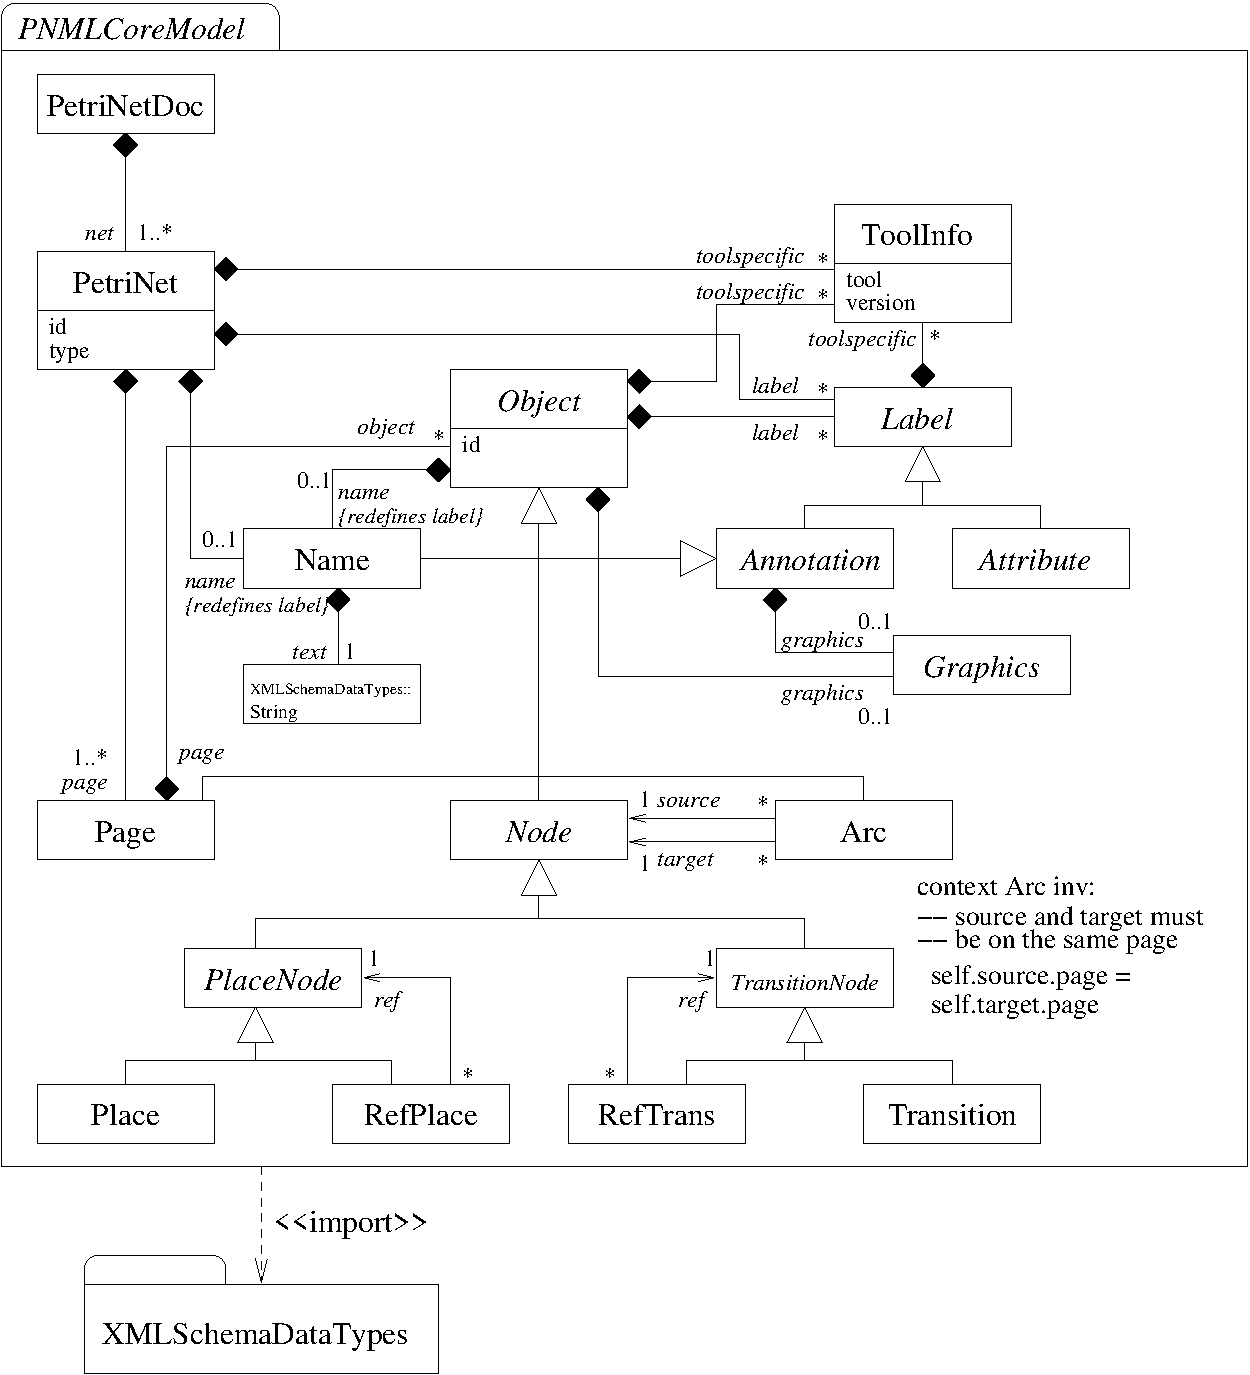
\includegraphics[scale=.58]{PNML_MetaModel}}
  \caption{The PNML core model of
    ISO/IEC~15909-2:2011 \cite{ISO-IEC:15909-2-2011}}
  \label{fig:MetaModel}%
  \index{PNML core model|DEF}
\end{figure}

Note that there is only one concrete type of label defined in the PNML core
model itself, which is the \emph{name} of an element.%
  \index{Petri net!Name|DEF}
All the other possible labels are defined in
separate Petri net type definitions, which are discussed in
Sect.~\ref{subsec:PNTD}.

In addition to the concepts and relations between them, the PNML core model
states also some restrictions on the structure of PNML models. For example,
there is a \emph{constraint}%
  \index{Constraint}
stating that arcs can connect only nodes that
are on the same page. This constraint if formulated as an \emph{OCL constraint}
in Fig.~\ref{fig:MetaModel}.
Note, however,
that there is no constraint in the PNML core model, which states that arcs must
run between a place and a transition or the other way round. The reason 
for not having such a constraint in the PNML core model is that there are
some kinds of Petri nets that would allow arcs between places or between 
transitions. This is why these kind of restrictions would be part of a
Petri net type definition.

Note also that the PNML core model does not specify concrete tool specific
extensions. It is up to a tool to define what it needs. But, any tool must be
able to read  -- and later write -- any tool specific extension; their contents
however, can be ignored.%
  \index{PNML core model|)}

\subsection{Petri net type definitions}
\label{subsec:PNTD}
\index{PNTD|(DEF}
As stated above, it is the purpose of a  \emph{Petri net type definition} to
define which labels are possible in a specific kind of Petri net, and also
to define some additional restrictions on the legal connections. Here,
we explain the idea of a Petri net type definition by the help of a simple
example: the definition of \emph{Place/Transition-Systems} (\emph{P/T-Systems}
in short).%
  \index{P/T-system|DEF}

The two additional kinds of labels for Place/Transition-Systems are the initial
marking for places, and the inscription for arcs.  The initial marking can be
any natural number (including 0) and the inscription for arcs can
be any positive number.  Figure~\ref{fig:PT-PNTD} shows the UML
model for these concepts and how they are related to the
concepts of the PNML core model.

\begin{figure}[hbt!!]
  \centerline{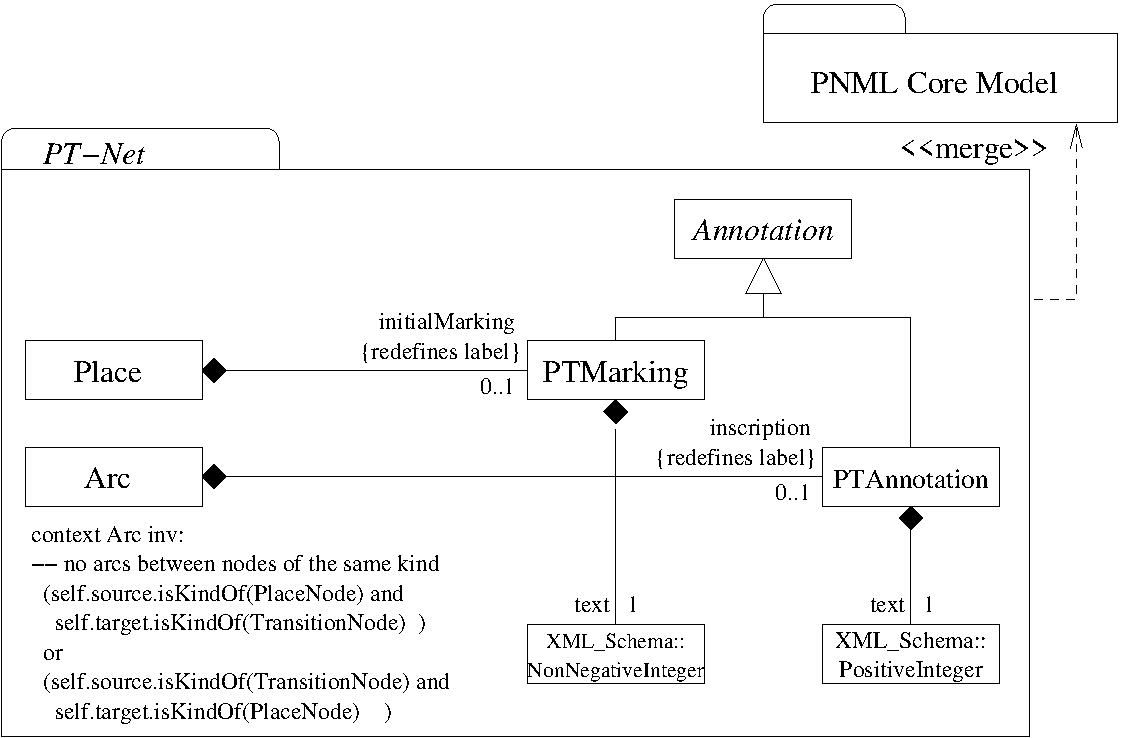
\includegraphics[scale=.60]{PT-PNTD}}
  \caption{The PNTD for PT-Nets}
  \label{fig:PT-PNTD}
\end{figure}

In Fig.~\ref{fig:PT-PNTD}, there is also one additional \emph{OCL constraint}.%
  \index{OCL constraint}
Without going into the details of OCL, this constraint states that
an arc must run from a place to a transition or from a transition to
a place. So, for P/T-Systems, it is no longer possible to connect places
with places or transitions with transitions.

A Petri net type definition, would typically also define how the new
concepts from Fig.~\ref{fig:PT-PNTD} would be mapped to XML. If not stated,
the ePNK will uses a default of how the new features are mapped to XML.
For the example above, this default mapping is good enough (and actually
compatible with ISO/IEC~15909-2).%
  \index{PNTD|)}

\subsection{Mapping to XML}
\label{subsec:XML-Mappings}
\index{PNML!XML format|(DEF}
As mentioned above, the PNML core model together with the model
for a Petri net type definition, define the concepts of a specific
kind of Petri net and how they can be connected. Therefore, these
models are the centerpiece of PNML. Still, PNML is an XML transfer
format for Petri nets. So, PNML defines how these concepts are saved or
represented in XML.  This is achieved by mapping every concept or feature of the
UML models to some XML construct. 


\begin{figure}[htbp]
  \centering
  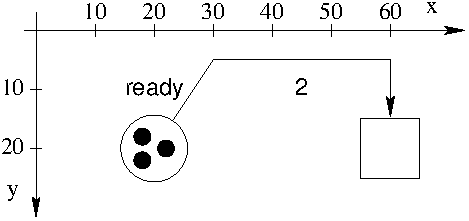
\includegraphics[scale=.5]{samplePTnet}
  \caption{A simple P/T-System}
  \label{fig:sample-net}
\end{figure} 

Here, we do not give these mappings, but rather 
show an example (for a detailed  discussion of the mappings,
see \cite{HKea09}). Figure~\ref{fig:sample-net} shows a simple example of a
P/T-System in its graphical representation (concrete syntax);
Listing~\ref{lst:sample-net} shows its representation in PNML's XML-syntax\footnote
  {We deleted some line-breaks to make this listing fit on a single page}.

\begin{figure}[p]
\lstinputlisting[language={[structured]PNML},keywordstyle=\underbar,label=lst:sample-net,%
caption={[PNML code of an example net]%
  PNML code of the example net in Fig.~\ref{fig:sample-net}}]%
  {samplePTnet.pnml}
\end{figure}

Note that the listing also shows an example of a tool specific extension:
the positions of the individual tokens in the place.%
  \index{PNML!XML format|)}%
  \index{PNML|)}

\section{ePNK: Objective}
\label{sec:Intro:Objective}

The main objective of the \emph{ePNK|DEF} was to build a tool that fully
supports the concepts of PNML, so that new Petri net types along with the mapping to
XML syntax can be easily plugged into this tool -- and to provide all the Petri
net type definitions for the types defined in ISO/IEC~15909-2:2011.

As soon as such a new Petri net type definition is plugged in, it
should be possible to load and save Petri net documents that contain
nets of these types. Moreover, there should be a graphical editor
that allows us to edit Petri nets of any plugged in Petri net type;
and the editor should be fully aware of all the features (annotations and
attributes) and the additional constraints of the plugged-in Petri net types.

For tool developers, the ePNK should provide an API to easily load and access
Petri nets from PNML files, to manipulate them, and to save them. Moreover, it
should be easy to plug in new functionality and \emph{applications}%
  \index{ePNK!Application}
for analysing Petri nets and for visualizing the results, and for manipulating
Petri nets or transforming them to other models or to code.

\section{How to read this manual}
\label{sec:Intro:Read}

In this manual, we will explain the features of the ePNK in more
detail. 

On the one-hand side, this manual covers the parts relevant for the
``end user'' who just wants to load, save and edit Petri nets of
existing types and use some existing or plugged in functionality
of the ePNK. In the rest of this manual, we call these ``end users'' just 
\emph{users}.%
  \index{ePNK!User|DEF}
All the information relevant for users of the ePNK
  can be found in Chapter~\ref{chap:users-guide}.


On the other-hand side, this manual covers the information relevant for
\emph{developers}%
  \index{ePNK!Developer|DEF} 
who are interested in using the ePNK for their
purposes: extending it by defining new Petri net types and their graphical
appearance, by defining new tool specific extensions, or by implementing
new functionality and applications. Chapter~\ref{chap:developers-guide} provides
the information relevant for developers who want to extend the ePNK.

Chapter~\ref{chap:tutorial} is a tutorial, which discusses the concepts
and the major steps of defining new Petri net types, their graphical
appearance, and a simple simulator application on top of it. The tutorial
goes into all the technical details, and is written in such a way that
it can be read independently from Chapter~\ref{chap:developers-guide}.

Chapter~\ref{chap:install} discusses the installation of Eclipse and
the ePNK as well as the major changes of version~1.2 of the ePNK 
with respect to version~1.0.

% In some future version of this manual, there will also be a part
% that discusses the architecture, the design, and some of the used technologies
% (and their  problems). These parts might be interesting for developers, but
% actually addresses people interested in model-based software development
% technologies that are used (and extended) in this project: EMF, GMF, Xtext,
% ExtendedMetaData, EMF Validation, and OCL. For now, we conclude this manual
% with Chapter~\ref{chap:inside}, which gives a brief experience report on the
% implementation of the ePNK and an overview of features of the ePNK that
% might be implemented in the future.

% During the development of the ePNK, we came across some problems and issues of
% PNML or ISO/IEC~15909-2. Chapter~\ref{chap:pnml-suggestions} will list and
% discuss these issues and make some suggestions for improving future versions
% of PNML or the definition of some specific Petri net types.
% Chapter~\ref{chap:pnml-suggestions} is mostly addressed to people interested
% in the standardisation process of ISO/IEC~15909 -- mostly concerning Parts~2
% and~3.
  
\cleardoublepage

%%%%%%%%%%%%%%%%%%%%%%%%%%%%%%%%%%%%%%%%%%%%%%%%%%%%%%%%%%%%%%%%%%%%%%%%%%%%%%%
%% Users' guide                                                              %%
%%%%%%%%%%%%%%%%%%%%%%%%%%%%%%%%%%%%%%%%%%%%%%%%%%%%%%%%%%%%%%%%%%%%%%%%%%%%%%%
\chapter{Users' guide}
\label{chap:users-guide}
\index{ePNK!User}

This chapter explains how to use the ePNK for creating, loading, saving, and
editing Petri nets, and also how to use some of its functions and applications.
Since new Petri net types can be plugged in, we try to point out the general
principles of these editors and how to use them. For the particular syntax of
some labels of a specific Petri net type, it might be necessary to refer to
the documentation of the specific Petri net type. We will discuss
these principles by some of the Petri net types that come with the basic version of
the ePNK; and we use high-level nets (in terms of the ISO/IEC~15909-2
\emph{High-level Petri Net Graphs}, or \emph{HLPNGs}%
  \index{HLPNG|DEF}
for short) to point out for which parts you would need to refer to the specific
documentation of the specific Petri net type.

\section{Eclipse as an IDE}
\label{sec:Eclipse-IDE}
\index{Eclipse|(DEF}
\index{Eclipse!IDE|(DEF}
For users who are new to \emph{Eclipse} and its \emph{IDE} (Integrated
Development Environment), we start with a brief overview of Eclipse's workbench.
Users who are familiar with Eclipse already can directly read on in
Sect.~\ref{sec:CreatingPetriNetDocuments}.

Once you installed and started Eclipse (see Chapter~\ref{chap:install}), you
see the Eclipse \emph{workbench}.%
  \index{Eclipse!Workbench|DEF}
Depending on the chosen \emph{perspective},%
  \index{Eclipse!Perspective}
the different parts can be arranged in different ways. But,
the principle behind is always the same. Figure~\ref{fig:workbench} shows an
example of the Eclipse workbench, with some numbers marking some parts, which
we discuss next.

At the top of Fig.~\ref{fig:workbench} marked by (1), you can see the
\emph{menu bar} and the \emph{toolbar}.%
  \index{Eclipse!Menu bar|DEF}%
  \index{Eclipse!Tool bar|DEF}
Here, you will find the menus and tools for all the standard functionality, such
as loading and saving files, and for standard editing operations. The
menus that are shown in the menu bar depend on your installation and
also on the editor that is currently active. For many operations,
there are also the standard shortcuts, like CNTRL-S (on the
Windows platform) for saving the contents of an editor to a file.  For getting
more information on that, you could chose the ``Help Contents'' in the menu
``Help'' in the menu bar, and read the ``Workbench User Guide''.

\begin{quote}
{\bf Note:} In automatically generated editors, such as the graphical
editor of the ePNK, the copy/paste functionality with CNTRL-C, CNTRL-V, and
CNTRL-X does not work properly. In order not to mess up models, by improperly
using cut/paste operations, the graphical editor of the ePNK does
not support copy/paste yet.
\end{quote}

\begin{figure}[hbt!!]
  \centerline{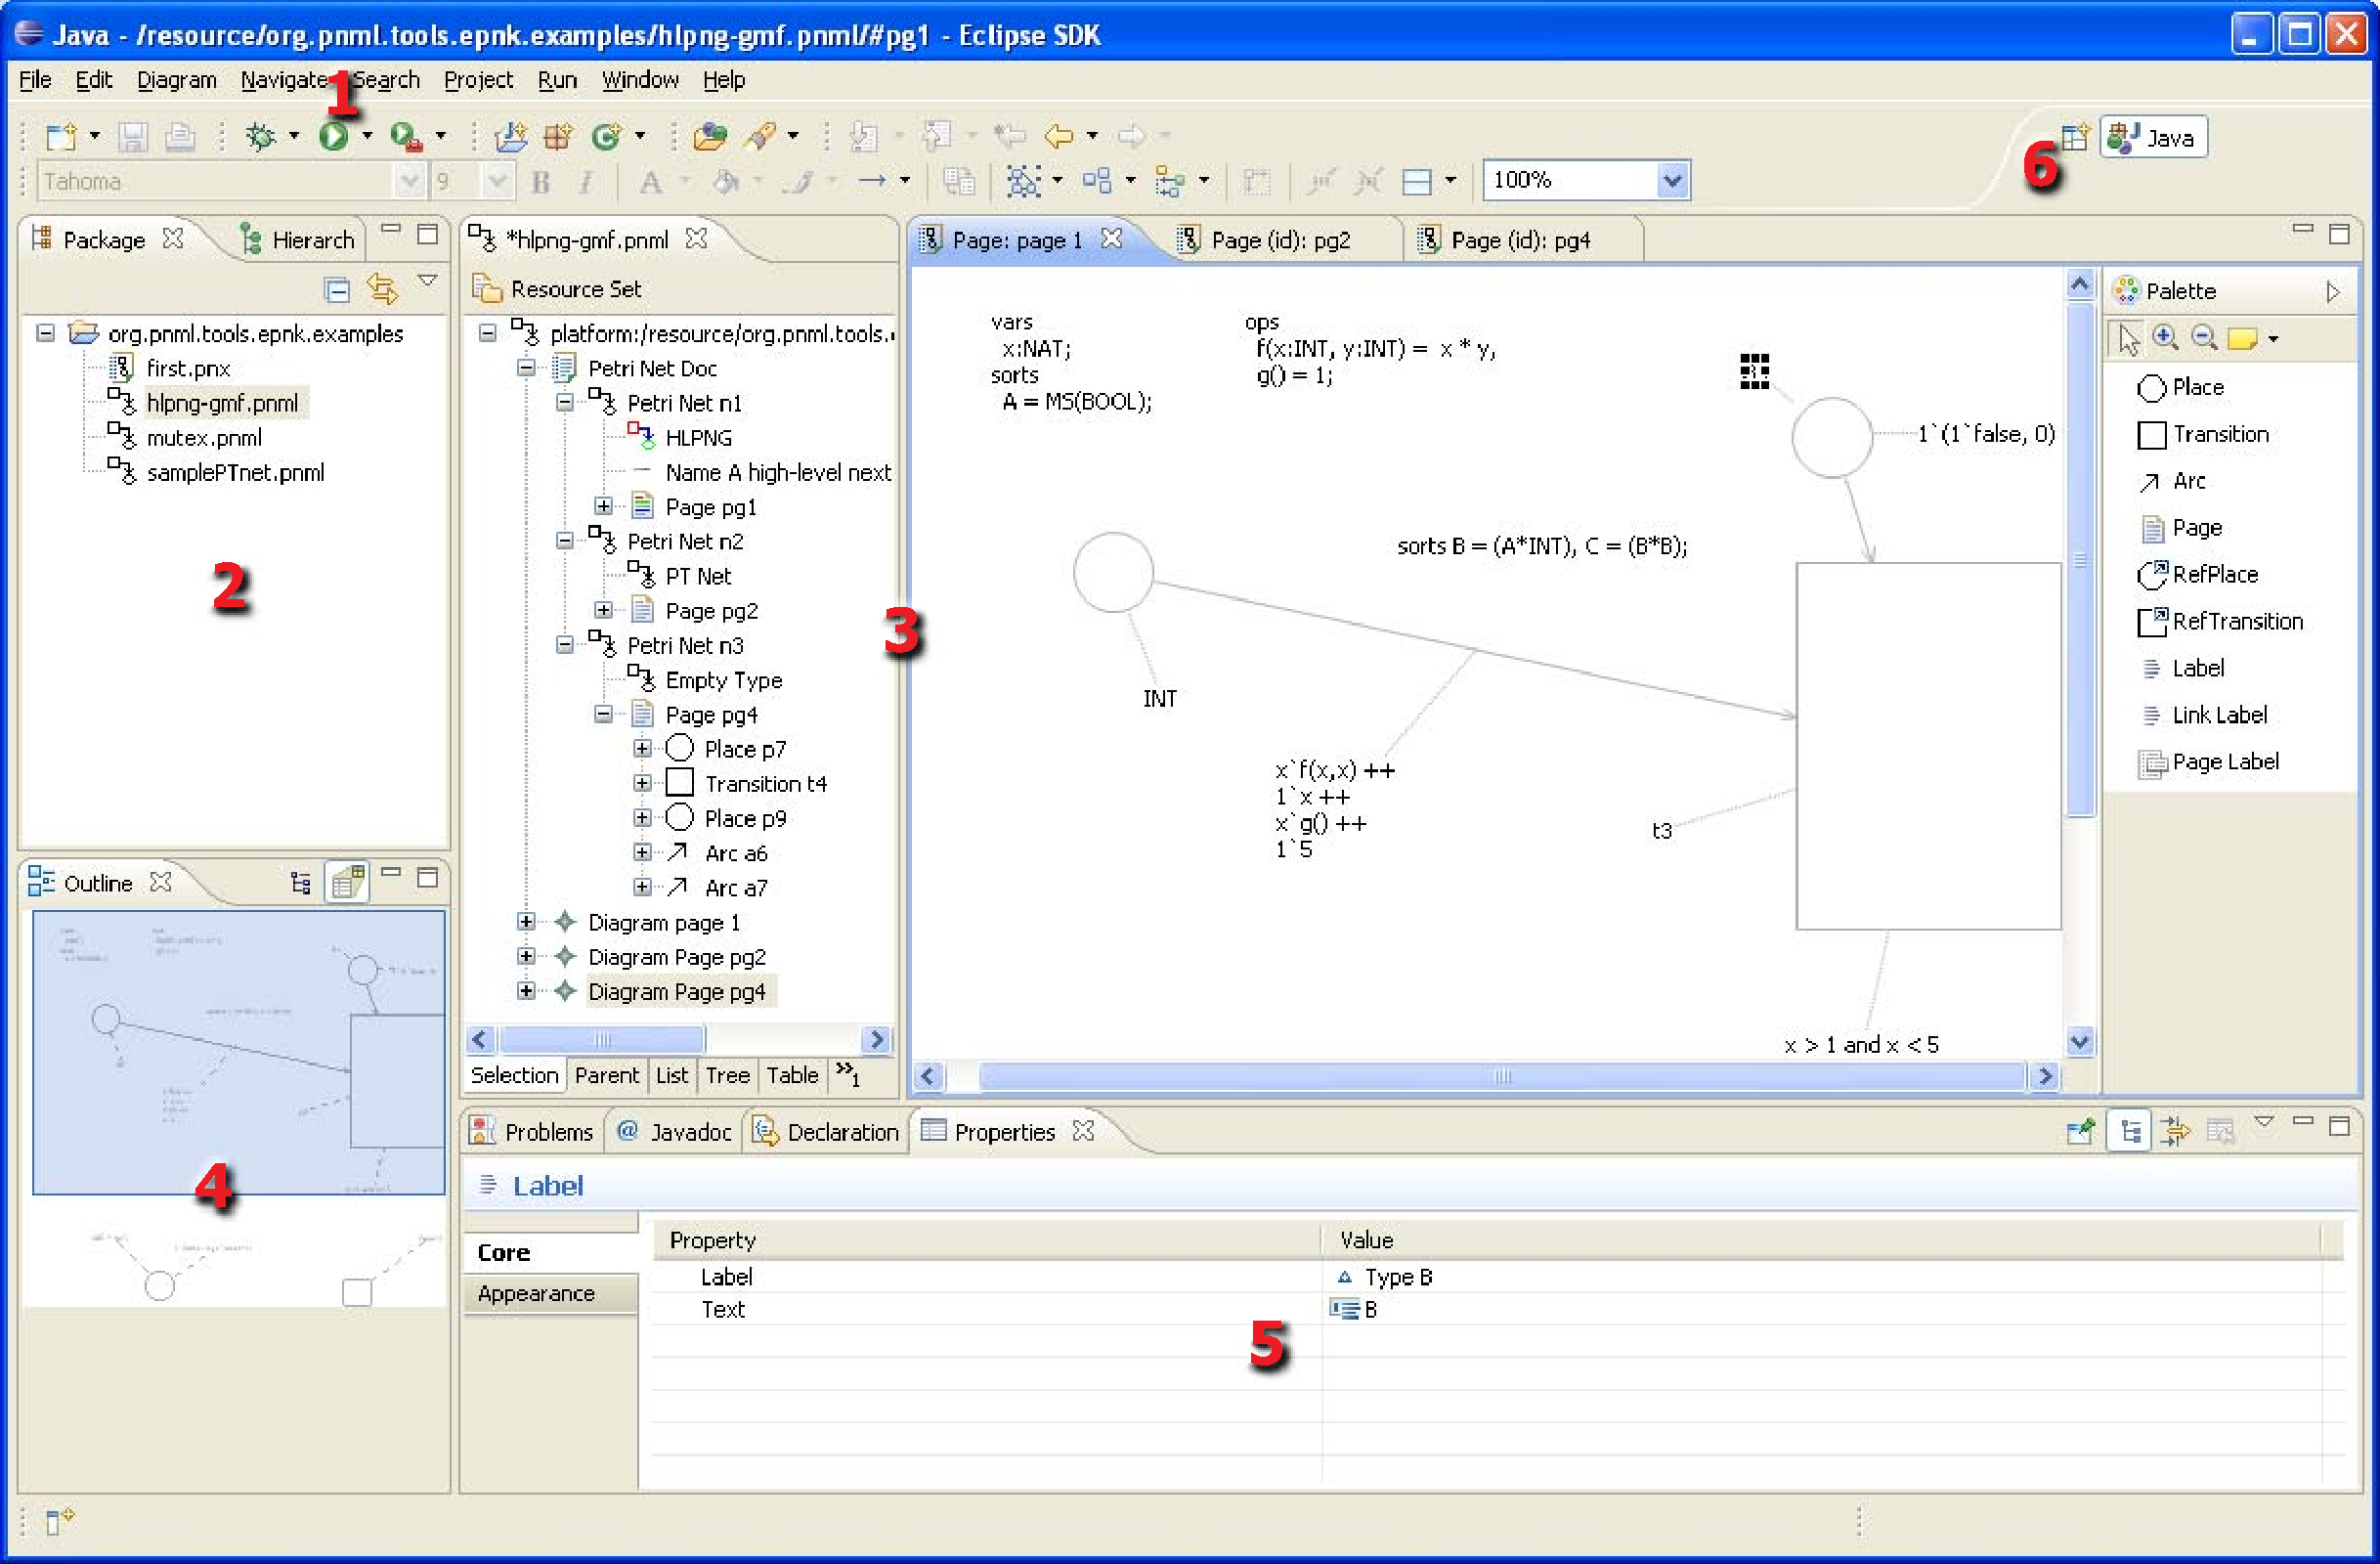
\includegraphics[scale=.30]{IDE-marked}}
  \caption{The Eclipse workbench}
  \label{fig:workbench}
  \index{Eclipse!Workbench}
\end{figure}

On the left-hands side, marked by (2), you can see the \emph{package explorer},%
  \index{Eclipse!Package explorer|DEF}
which gives you access to all the files in your workbench. The package explorer
can be used for browsing through the existing files and for manipulating,
renaming, copying, moving, and deleting them. This is very much like the file
explorer of your operating system. Eclipse actually has different kinds of explorers,
depending on the perspective and the user's preferences. The package explorer is
made for Java development projects. For our purposes, any of these explorers
would do, like for example the ``navigator'' or the simple ``project explorer''.
To find and open one of these other explorers, you can use the menu ``Show View'' in the
menu bar menu ``Window''. All these explorers have some important concept
in common, which concerns the organisation of files in the workbench: the
top-level ``folders'' are actually not folders, but they are \emph{projects}.
This is relevant only when creating these projects. You can create a folder
or file in the workbench only after you have created some project; this can be
done via the ``File'' menu or by a right-click in the explorer and then
selecting ``New''$\rightarrow$``Project''. Note that in the dialog, you can
create many different kinds of projects; for us the kind ``Project'' in
category ``General'' will do. Then, files can be created within
this project. 

In the center (3), you can see the \emph{editor area} of Eclipse. This is%
  \index{Eclipse!Editor|DEF}
where all the editors that are started in Eclipse will be opened. Note that
there can be many editors open at the same time (in our example, there are four
editors open). Typically, you can see only one at a time and the others are
hidden below it. But, you can move the editor tab to some border of the editor
area, so that you can see the contents
of two or more editors at the same time. In our example, there is
a tree editor of a complete Petri net document open on the left-hand
side, and, on the right-hand side, you can see one specific page open
in a graphical editor (the graphical editors for some other pages are hidden
beneath). Note that, even though there can be many editors open and even visible
at the same time, there will always be only one editor that is active. This
editor and what is selected in it determines what you see in some other
views. For example, you can see the \emph{outline view} (4)%
  \index{Eclipse!Outline view}
of the page or you can see the
property of the currently selected element in the \emph{properties view} (5)%
  \index{Eclipse!Properties view}
at the bottom.  In order to open an editor on some resource in the explorer,
you would, typically, double click on the resource you want to open. This will open
the \emph{default editor}%
  \index{Eclipse!Default editor|DEF}
on the selected resource. You can also use the right mouse button on a resource
to open a pop-up menu and then select ``Open with'' 
to select a specific editor for this purpose. The way of editing the contents
of a resource depends on the kind of editor; generally, it is straightforward.
Saving the file can typically done by a shortcut (like CNTRL-S) in all 
editors (or via the ``File'' menu in the menu bar).
An editor can be terminated (closed) either by clicking the close
symbol on the tab of the editor or via the ``File'' menu in the menu bar.

Most editors support undo and redo of the latest changes, which you can
access via the ``Edit" menu or via the CNTRL-Z and CNTRL-Y shortcuts.

Note that the graphical editor of the ePNK cannot be initiated directly from
the explorer since the resource could have many pages and a page is
not the top-level element. When you open a PNML file, a tree editor
will be opened that shows the structure of the Petri net. The graphical
editors for a page of a Petri net can be opened by a pop-up menu (right
mouse button) on pages in the tree editor for Petri nets or by a double
click on the page (see Sect.~\ref{sec:graphical-editor} for details).

All the other areas of the workbench are% 
  \index{Eclipse!View|DEF}
\emph{views}\footnote
{Actually, also the resource browsers are views.}%
. In Eclipse, views are used for many different purposes. The
views that are most relevant for us, are the \emph{outline}%
  \index{Eclipse!Outline view|DEF}
(4), the \emph{properties}%
  \index{Eclipse!Properties view|DEF}
(5), and the \emph{problems view}% 
  \index{Eclipse!Problems view|DEF}
(not visible in
Fig.~\ref{fig:workbench}). The outline gives an overview of the contents of
the currently active editor and, in case of a graphical editor, allows us to
quickly move around the visible area of this editor. The properties view
shows some details of the currently selected element in the editor; in many
cases, the properties view also allows us to edit some properties. Note that,
initially, the properties view might not be open. You can, typically, open it
from the active editor via a context menu on the right mouse button:
In the pop-up menu that opens, there will be a menu ``Show Properties
View'', which opens the properties view. You can also open
the properties view via 
``Window''$\rightarrow$``Show View''$\rightarrow$``Others ...'' and
then selecting ``Properties'' in the category ``General''.

We mentioned already that the Eclipse workbench can appear
in different ways, which is defined by the chosen \emph{perspective}%
  \index{Eclipse!Perspective|DEF}
(and some user-specific settings). The perspective can be changed via
the tools at the top-right of the workbench, which are marked with (6)
in our example. We do not need to change it; but if, for whatever reason, you
end up in a wrong perspective, by clicking on the left symbol,
you can open the ``Open Perspective'' dialog. There, you can
select the perspective ``Resource'' or, if you like, ``Java'' (which is
the default perspective).
 
If you are interested in more details in the Eclipse workbench,
you can have a look into the Eclipse help
(``Help''$\rightarrow$``Help Contents'') or at one of the
many books or online articles;
\url{http://www.vogella.de/articles/Eclipse/article.html} could
be a start.%
  \index{Eclipse|)}%
  \index{Eclipse!IDE|)}

\section{Creating Petri net files}
\label{sec:CreatingPetriNetDocuments}

This section explains how to create new ePNK files. Note that there
are two formats in which the ePNK can save a Petri net. The first and
recommended format is PNML. The second format is the XMI-serialisation of the
PNML models, which we call PNX.  Note that PNX, is part of the ePNK since XMI is the
standard serialisation mechanism of the EMF technology used for implementing
the ePNK and, therefore, came for free. Whether PNX really should be a part of
the ePNK distribution is yet to be seen. Therefore, the focus of
this users' guide is on PNML.

The easiest way of getting started with the ePNK is obtaining existing PNML
files from somewhere else and just copy them to the workbench. For example, you
could get some examples from the ePNK home page: 
\url{http://www2.compute.dtu.dk/~ekki/projects/ePNK/}. You can also use a text
editor and create a simple text file with file extensions ``.pnml'' and insert
the single line
\begin{lstlisting}[language={[structured]PNML},keywordstyle=\underbar]
  <pnml xmlns="http://www.pnml.org/version-2009/grammar/pnml"/>
\end{lstlisting}
to this file, which is an empty Petri net document without any nets in it.

The ePNK also provides you with a wizard for creating a PNML document.
Like all Eclipse creation wizards, this wizard is started via the ``New''
menu, which can be either accessed by the ``File'' menu from the menu bar or via
the pop-up menu that opens on a click to the a right mouse button in the
explorer.
Then, select ``Other...'' (the short-cut to that would be pressing
CNTRL-N in the explorer) and in the newly opened ``Select a wizard''
dialog choose ``PNML Document''%
  \index{PNML Document|DEF}
from the ``ePNK'' category and press
``Next''. In the next dialog, you must choose a name and, if you
want, you can choose a different folder in which this file should
be created. Pressing ``Finish'' will create the file; then, the
newly created file will be opened in a tree editor (see
Sect.~\ref{sec:tree-editor});%
  \index{ePNK!Tree editor}
note that you also can continue the
creation process by pressing ``Next'', which will allow you to chose an
XML-Encoding.  Note that, in the dialog with the encoding, there
is also a field asking for the ``Model Object''; but you cannot
choose anything here since PNML, in contrast to other formats,
has a fixed root object that cannot be changed: ``PetriNetDoc''. 

Note that in the same wizard category ``ePNK'' there is another
wizard called ``PNX Document''.%
  \index{PNX Document|DEF}
When you use this wizard, a PNX file
will be created. In this wizard, you can select a root element different
from the PetriNetDoc -- but this would be reasonable only in very special cases
(and when you know exactly what you are doing).
 
\section{The tree editor}
\label{sec:tree-editor}

\index{ePNK!Tree editor|(DEF}
As mentioned earlier, the ePNK provides two kinds of editors
for Petri nets: the \emph{tree editor}, which allows us to create,
modify, and delete all parts of the Petri net in a tree-like
structure; and the \emph{graphical editor}%
  \index{ePNK!Graphical editor}
in which a page
of a Petri net with its places, transitions, and arcs can
be edited in a graphical way. Clearly, the graphical editor
is more convenient for editing pages than the tree editor.
But, other parts like for example the page structure and the
complete Petri net document are more convenient to edit in the
tree editor. This is why there are two different editors in the ePNK.
The graphical editor for pages is always started from a
selected page -- either in the tree editor or in the graphical
editor. When opening a PNML document from the resource explorer,
it will always be the tree editor that opens. A graphical editor
can be opened by a double click on a page element in an already 
open editor.

\subsection{The tree editor: Overview}
Let us have a closer look at the tree editors first.
Figure~\ref{fig:tree.editors} shows the Eclipse workbench with
two PNML documents open in tree editors. The right one shows the tree editor
opened with the PNML file (``test.pnml'') with the single line as discussed in
Sect.~\ref{sec:CreatingPetriNetDocuments}. Therefore, it contains only the
Petri net document element without any contents. The other PNML document, which
is open on the left-hand side (``hlpng-gmf.pnml''), shows a Petri net document
with three nets that have different types.
 
\begin{figure}[hbt!!]
  \centerline{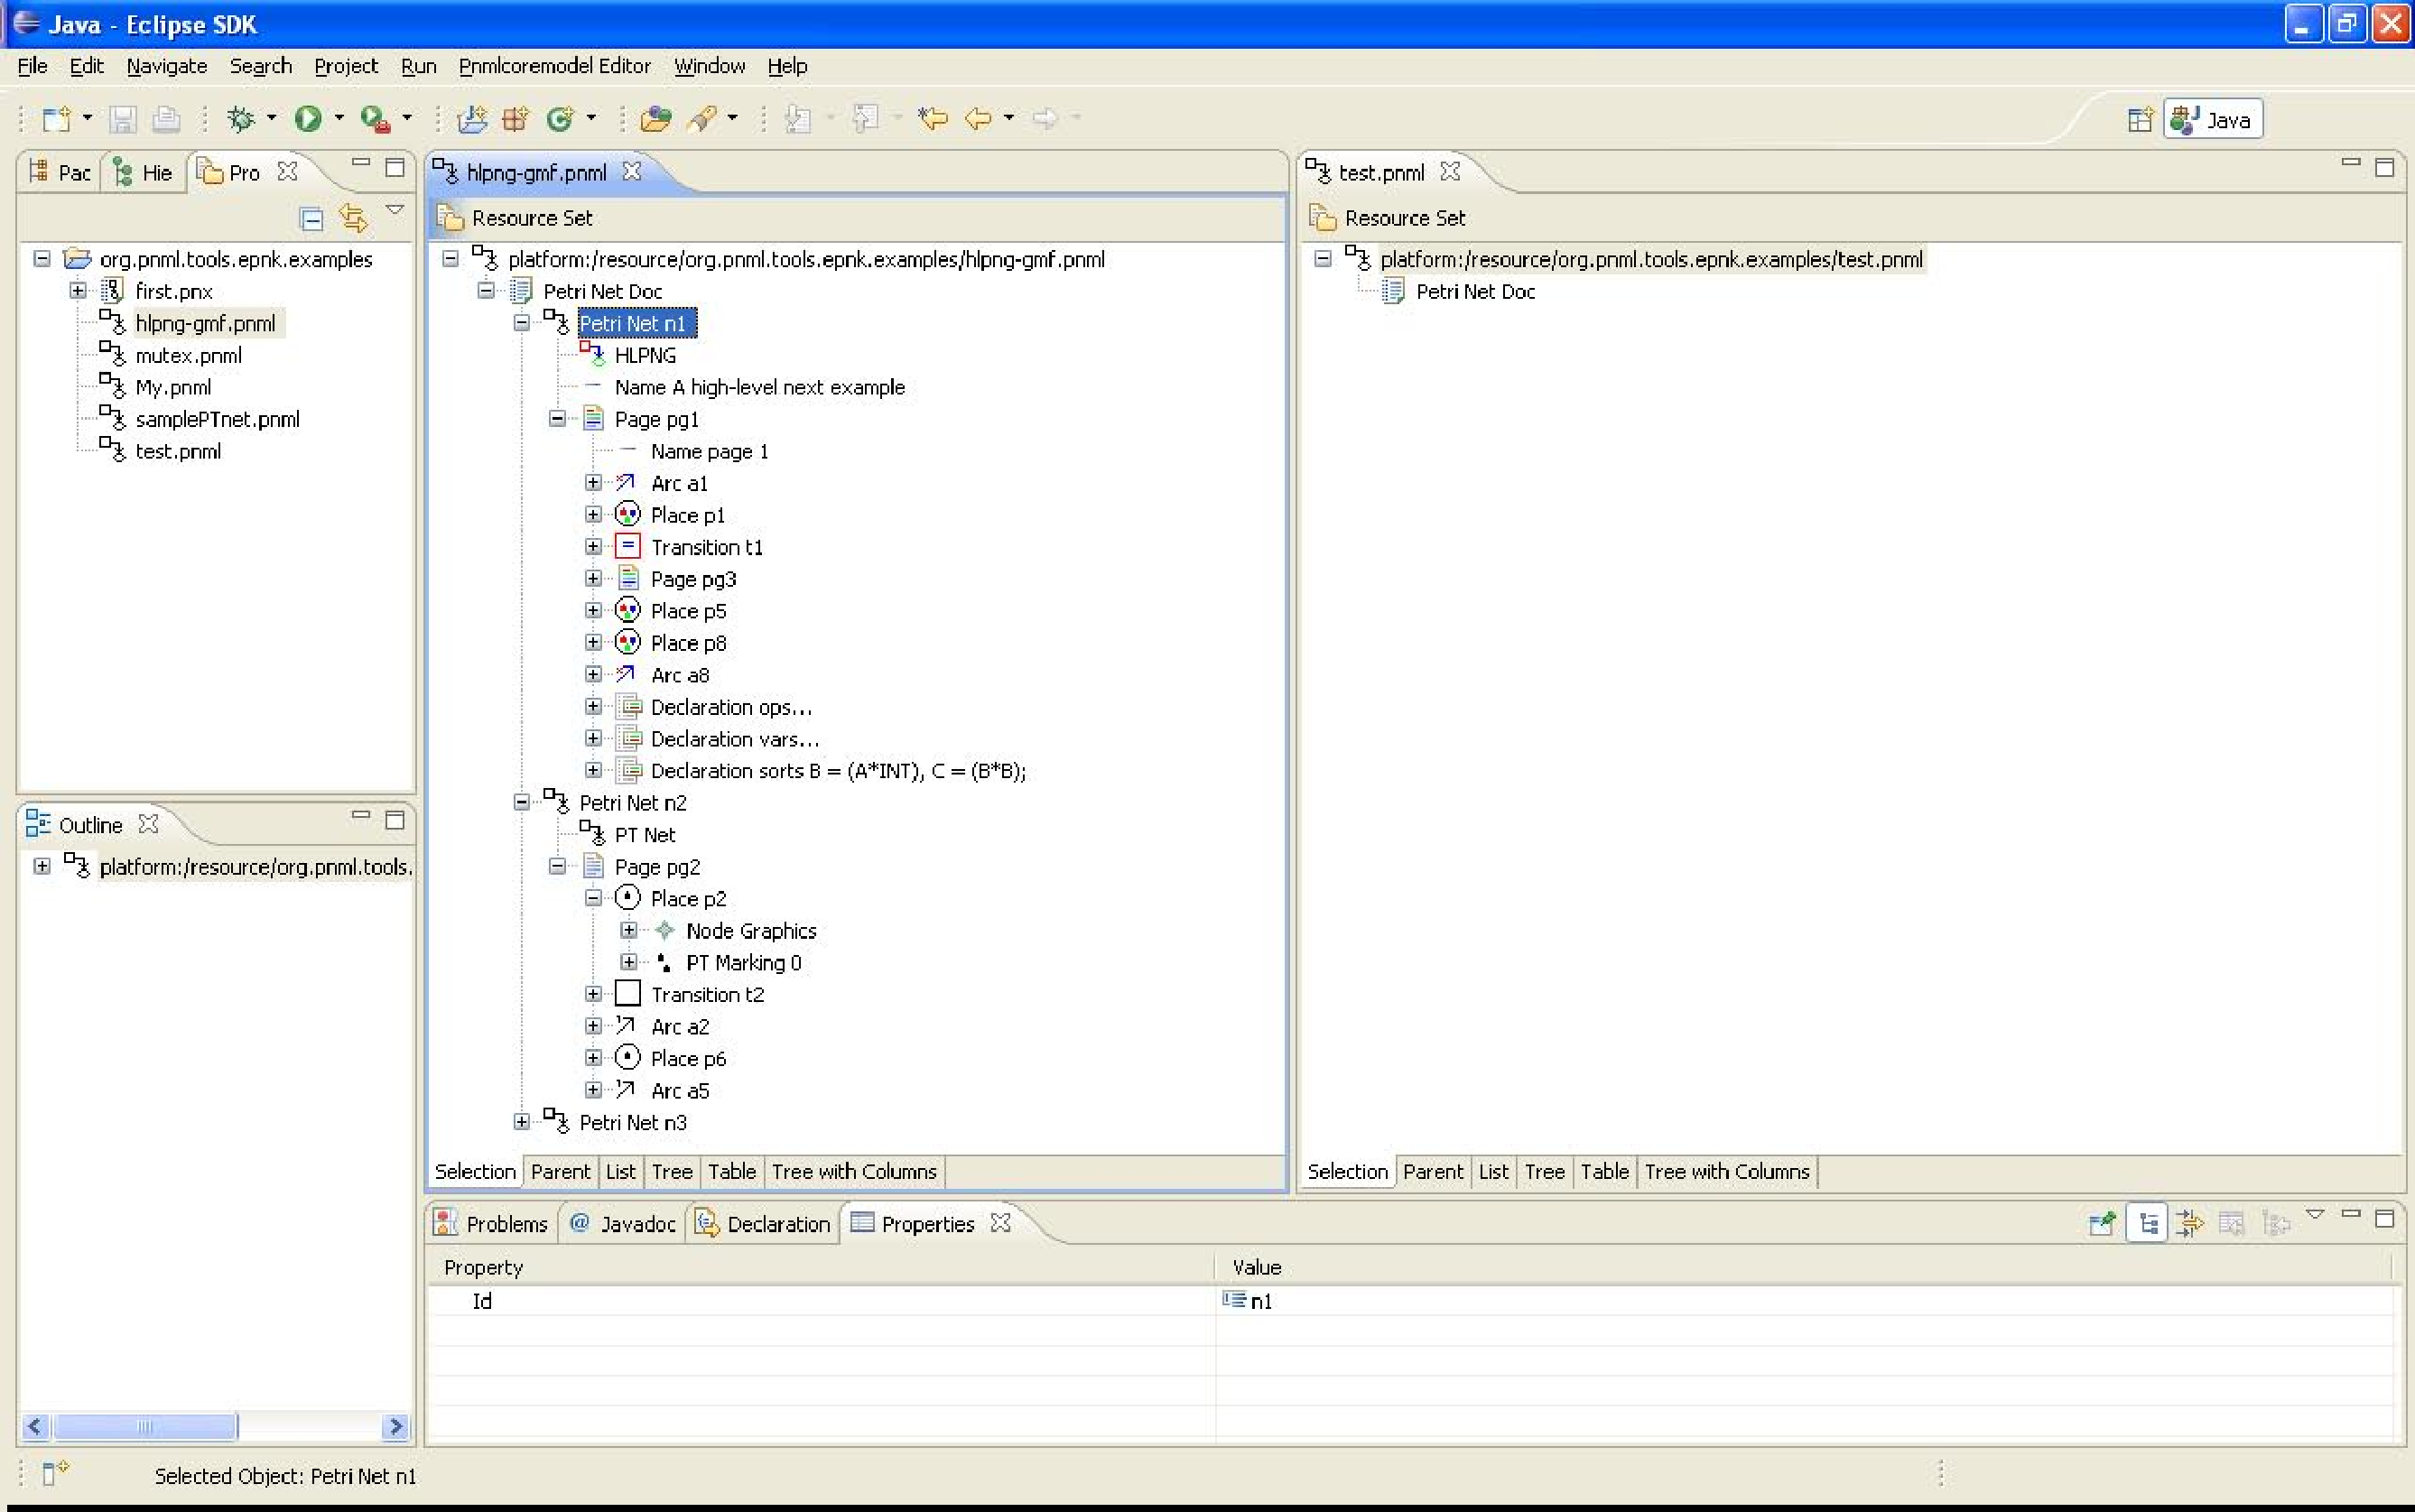
\includegraphics[scale=.28]{TreeEditors}}
  \caption{Two Petri net documents in tree editors}
  \label{fig:tree.editors}
\end{figure}

These documents were opened from the explorer by a double click\footnote
 {Remember, that you can use the pop-up menu to make an explicit choice
  by which editor you want to open the file. This way, you can open
  the file with a text editor, so that you can see the PNML
  it produces. On a double click, the file is opened
  with the editor you had selected the last time.}
on the respective file in the workbench's explorer. Let us briefly go through
what you see in the Petri net document ``hlpng-gmf.pnml''.  The top-line shows the
actual \emph{resource}%
  \index{Eclipse!Resouce|DEF}
or file in which this document is stored; the second
line is the symbol for the Petri net document itself -- all documents will
follow this structure in the tree editor. Then you can see that
there are three Petri nets contained in this document (with \emph{ids}%
  \index{ePNK!id}
n1, n2, and n3); the last net is actually not folded out because
its was not fitting to the screen. The first line below the 
Petri net is the type of the Petri net. The first net
is a high-level net, which is named \emph{HLPNG}%
  \index{HLPNG}
according to ISO/IEC~15909-2;
the second net is a Place/Transition-System, called PTNet according
to the standard. You can also see that the nets contain places, transitions,
and arcs, which are indicated by corresponding icons. You can also see
some pages and sub-pages.  Note that the icons for the places, transitions,
and arcs are different for the two different Petri net types, so that it
easier to distinguish them on a first glance. In the properties view at the
bottom, you can see the properties of the currently selected element, which is
Petri net n1; the only property is its id. Note that this net has a
name; this, however, is not shown as a property, but as a \emph{child element}%
  \index{Eclipse!Child element|DEF}
of the net, which is true for all labels of Petri nets. In this case, the name is 
``A high-level next example''.

\subsection{Creating elements}
\label{subsec:creating-elements}

You can unfold all the sub nodes (children) of the net and this way
inspect the complete document in all details. More importantly, however,
you can create the basic elements of the Petri net document. You can
create new nets (along with their type) and their pages. And from there, you
would use the graphical editor to draw the rest.  This basically works by
inserting \emph{child elements}.%
  \index{Eclipse!Child element|DEF}
Inserting a child element is done by
right-clicking on the element to which you want to add a child, then selecting
``New Child'' in the dialog that pops up, and then selecting the appropriate
element. Figure~\ref{fig:new-child-element} shows the pop-up dialog when
inserting a new Petri net to the Petri net document.

\begin{figure}[hbt!!]
  \centerline{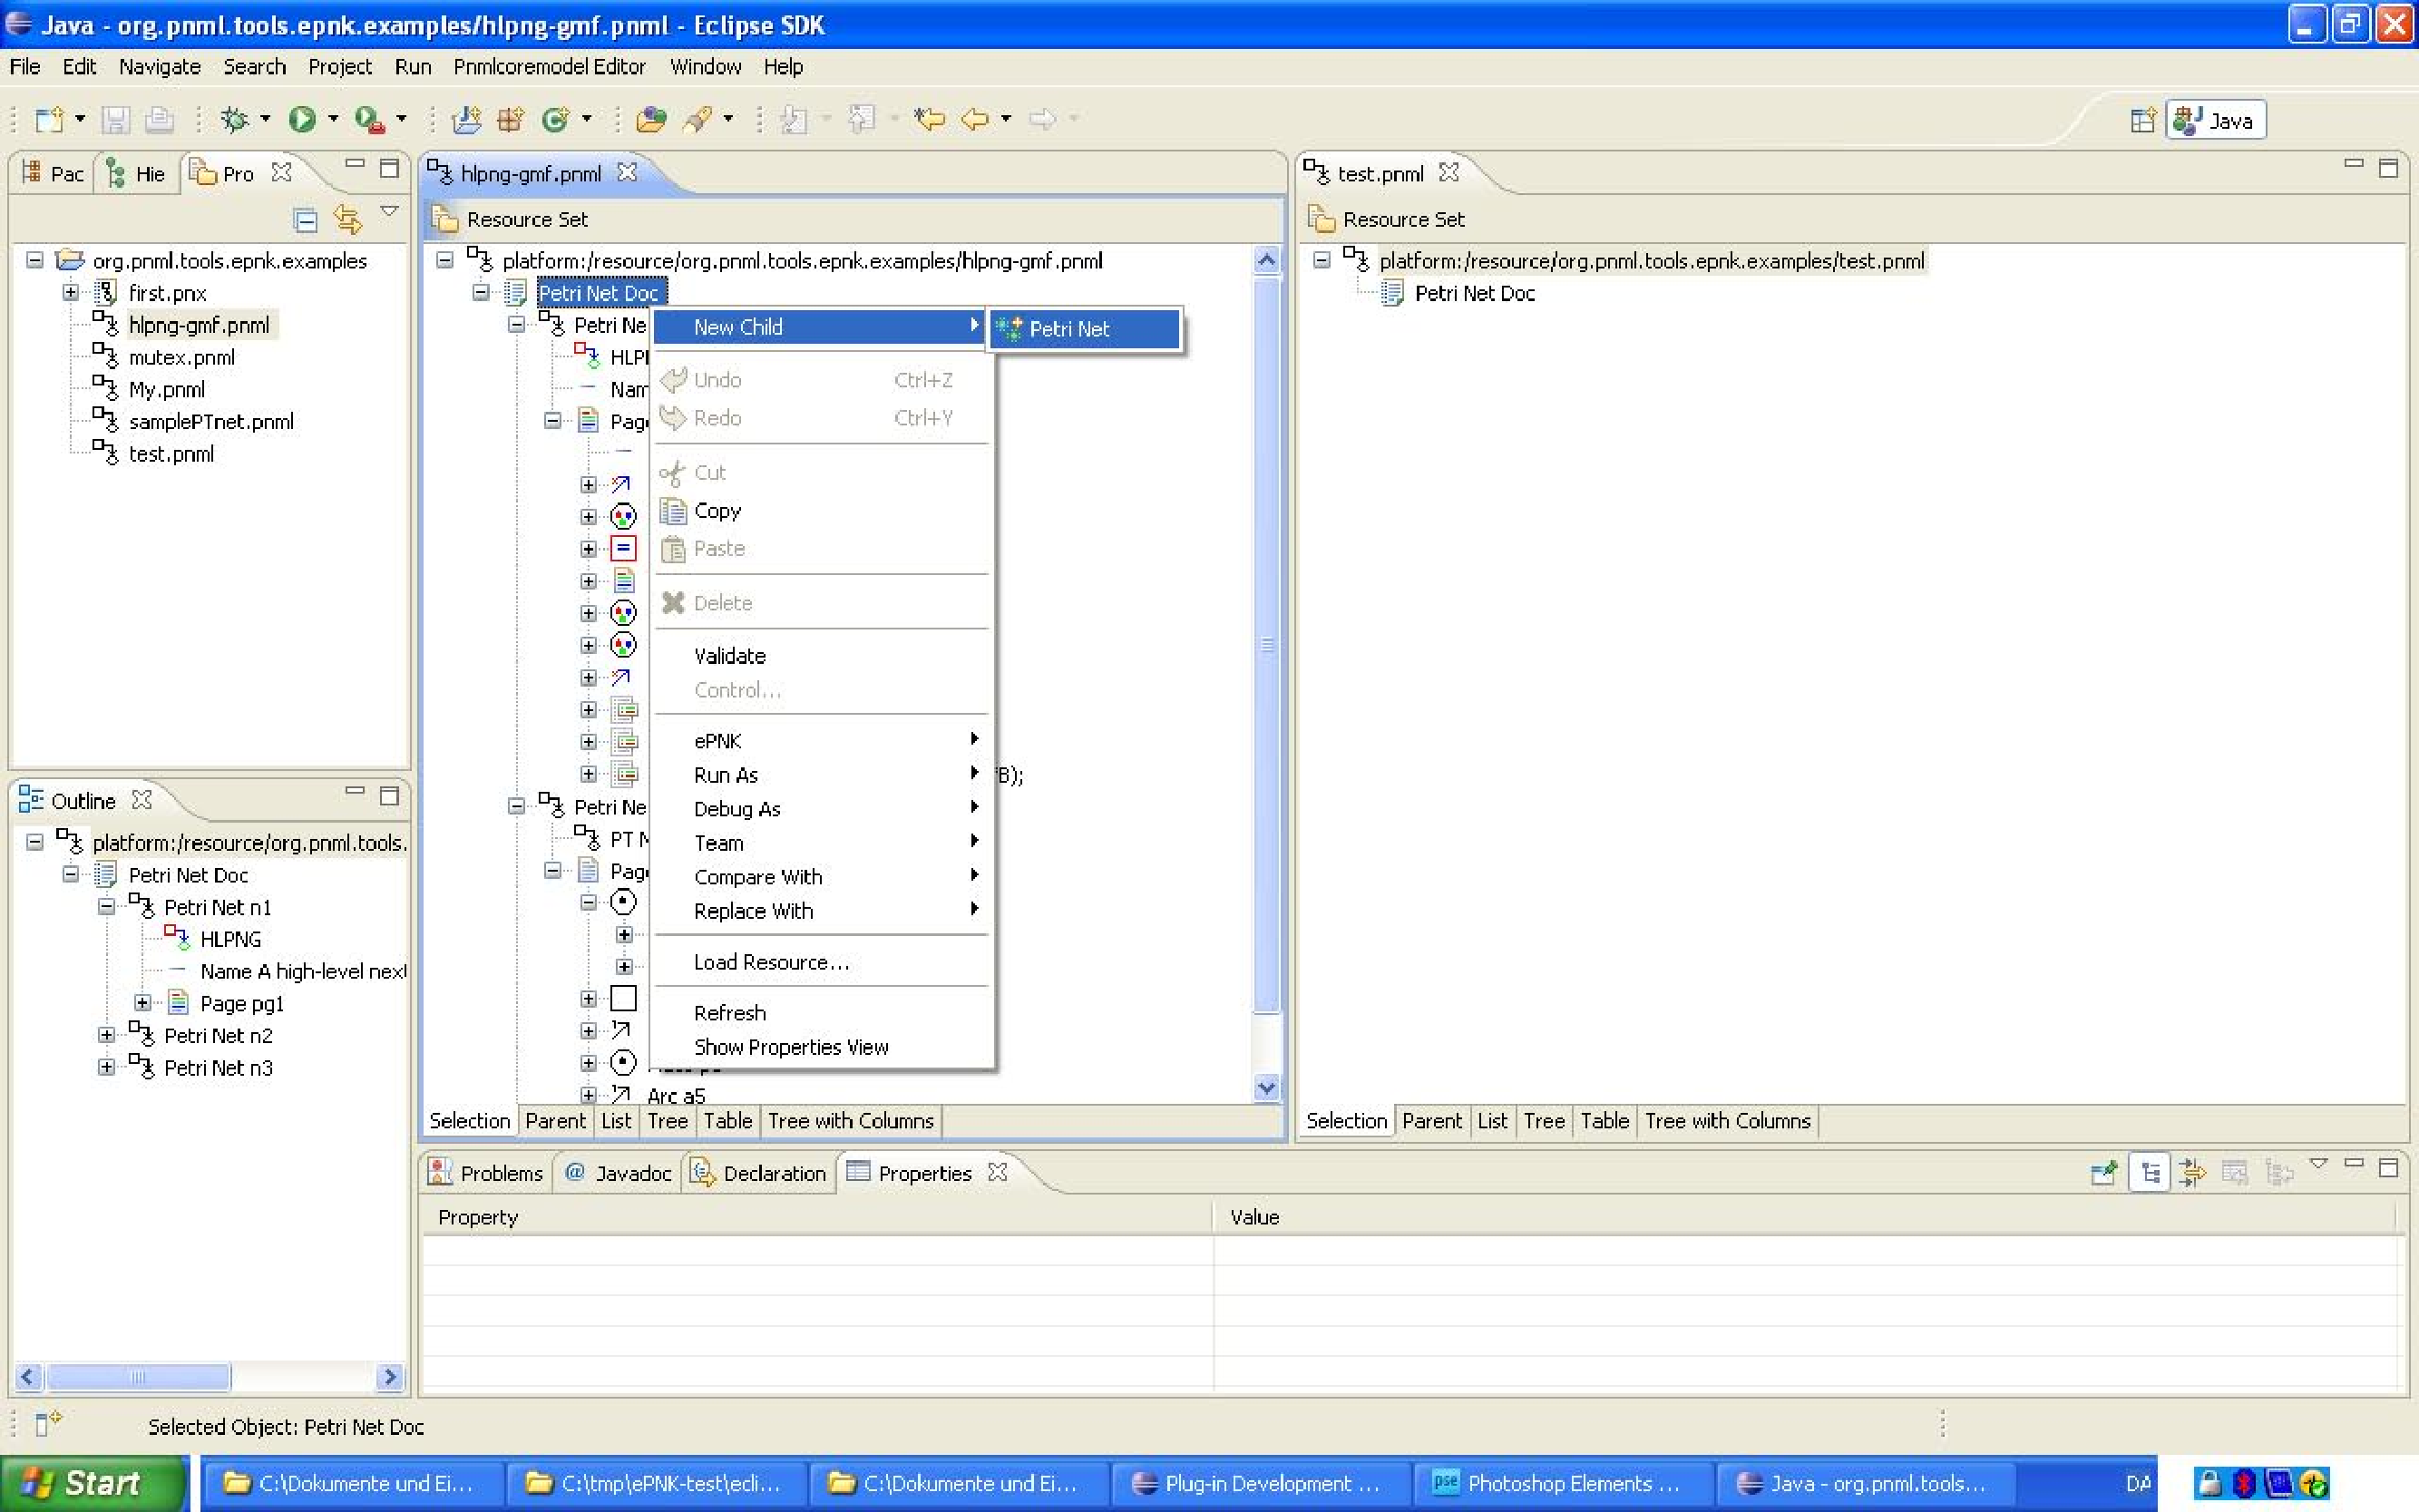
\includegraphics[scale=.28]{NewChildElement}}
  \caption{Pop-up menu when inserting a new Petri net}
  \label{fig:new-child-element}
\end{figure}

Note that this dialog will show all available Petri net types, from which
you will need to select. Then a new net of that type will be created. Note
that the created net will contain a child element, which represents
the type of this net. You should never delete or change this net type
manually\footnote
  {Unless you know exactly what you are doing.}.
You will find some more information on the Petri net types that
are deployed together with the ePNK in Sect.~\ref{sec:petrinettypes}. 

After you have created a new Petri net, the name of the net and new
pages can be inserted to it by via the ``New Child'' pop-up menu on the
selected Petri net similar to creating the net -- just select the
kind of element you want to create.

\subsection{Saving the document}
\label{subsec:save-documents}

As discussed in Sect.~\ref{sec:Eclipse-IDE}, you can save the net via the
``File'' menu or with the CNTRL-S shortcut. Note that saving the net
must be done -- and can be done only -- in the tree editor. Therefore,
only the tree editor shows the dirty-flag, when the editor contains
unsaved changes.

\subsection{Validating and correcting the document}
\label{subsec:validation}
\index{ePNK!Validation|(DEF}

Before saving a PNML document, it is a good idea to \emph{validate} the
net. This will check whether all the constraints that PNML and the
respective Petri net types imposes on the Petri net document are met. It is
possible to save a document that does not properly validate, and you would
be able to load the file again. But, if you save a file that
does not properly validate, you cannot be sure that the saved document
is ISO/IEC~15909-2 conformant PNML, and other tools might not be able to load
it.

There are many things that can be wrong and need validation
on a Petri net document. Most of them are type specific (such as the requirement
that an arc must run from places to transitions or the other way round only);
these Petri net type specific constraints will be discussed in
Sect.~\ref{sec:petrinettypes}. But, there are also some general constraints:
\begin{itemize}
  \item Every Petri net object must have an id and this id must be
        unique in the scope of this document.
        
  \item Arcs may only connect nodes which are on the same page (as
        long as you are using the graphical editor, this constraint
        cannot be violated; but if you do changes in the tree editor,
        this could be violated).
        
  \item There must not be cycles on the references between reference
        nodes, and all reference nodes must refer to a node.
        
  \item A reference node must refer to a node within
        the same net.  
\end{itemize}

In order to identify which constraints are violated, you can use the
validation feature. Click on the right mouse button on the Petri net
document; then, in the pop-up menu, select ``Validate''. The result
of the validation will be shown in a dialog; the results of the validation
is also visible in the \emph{problems view}\footnote
  {If the problems view is not open, you can open it by
   ``Window''$\rightarrow$``Show View'' $\rightarrow$``Problems''.}%
  \index{Eclipse!Problems view}
after the validation as shown in Fig.~\ref{fig:validation}. Most of these
errors are actually coming from high-level nets. But, there is also a general
constraint violated in this example: some IDs collide (line 5 and 6 in the
problems view), which means that the same ID is used twice in this document.

Note that you can double-click on the individual problems in the problems
view. Then, an editor is opened with the element to which this problem refers to
selected. If there is a graphical editor open for the page that contains 
the element with the error, the ePNK will show the selected element in the
graphical editor; if there is not graphical editor open with that element,
the element will be shown in the tree editor. 

\begin{figure}[hbt!!]
  \centerline{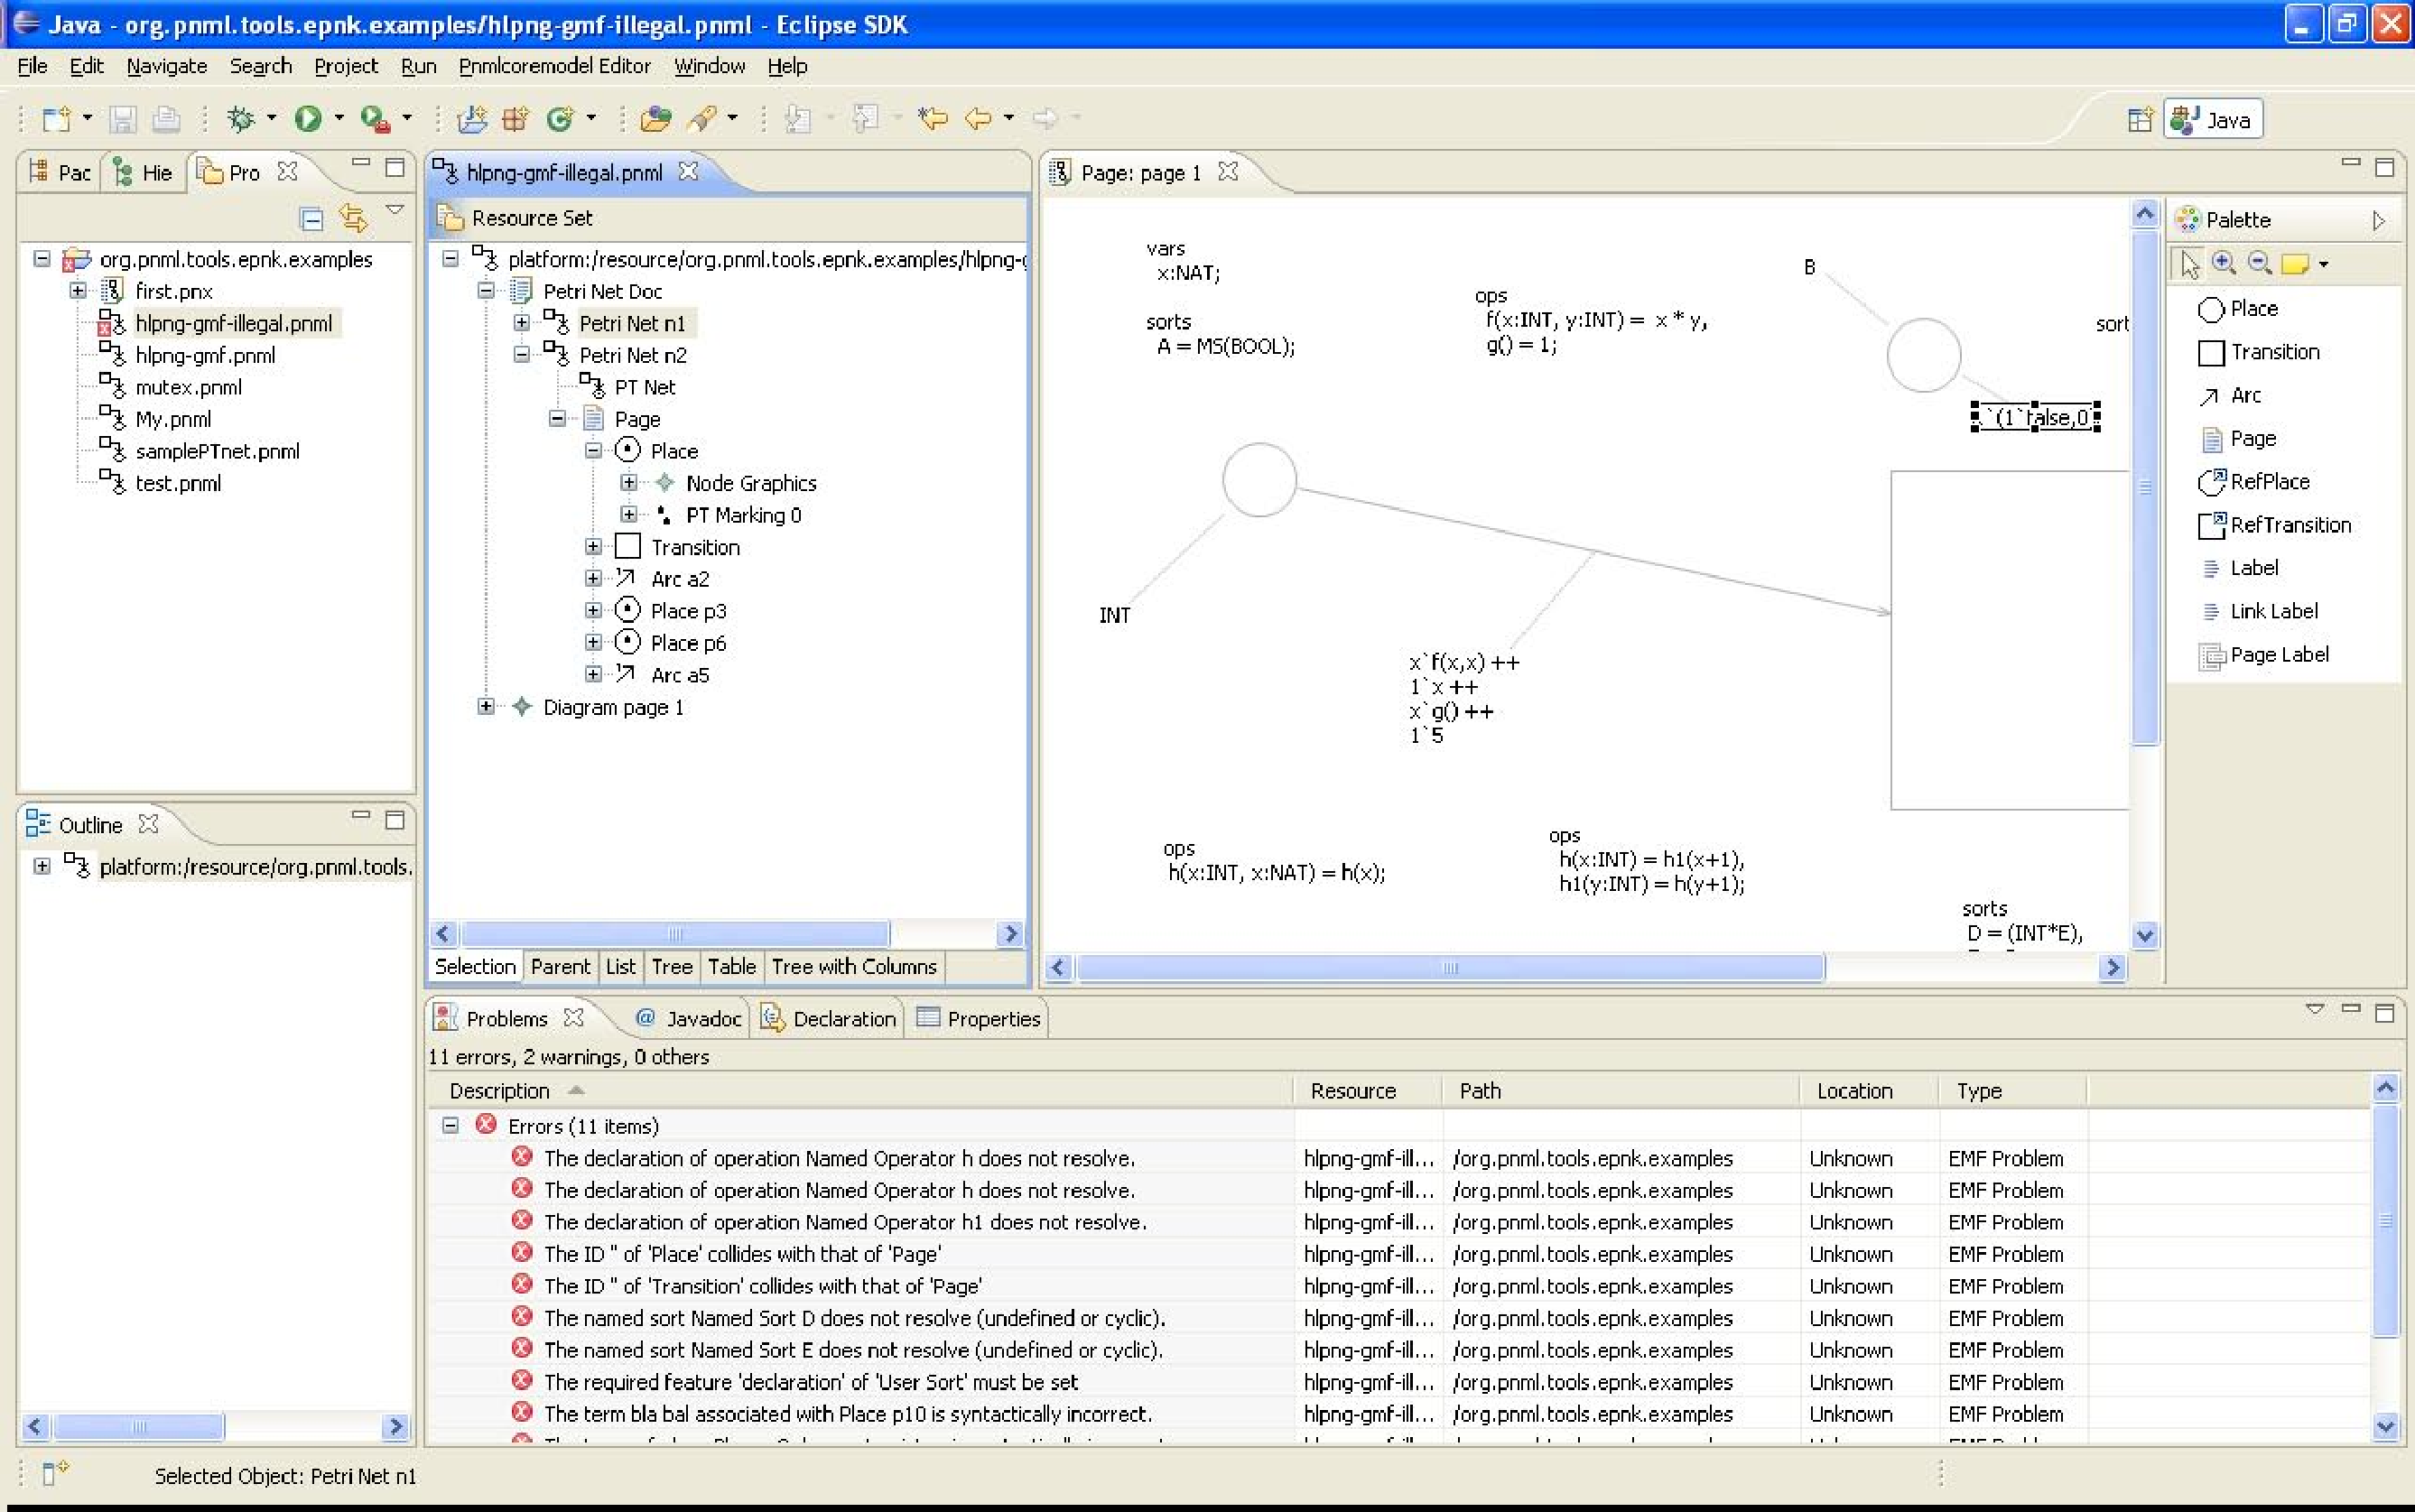
\includegraphics[scale=.25]{Validation}}
  \caption{The problems view with many constraint violations}
  \label{fig:validation}
  \index{Eclipse!Problems view}
\end{figure}

In order to reduce the number of errors, you can also do a validation
on sub-elements of the Petri net document, which could be a net
or even a single page. Ultimately, however, you must validate
the complete Petri net document.

In our example, there are some problems that
can be fixed automatically. For example, ids can be set automatically.
The ePNK provides an action for this. To this end, select the Petri net
document, click the right mouse-button, and then select
``ePNK''$\rightarrow$``Add missing IDs'' in the%
  \index{ePNK!id|DEF}
pop-up menu. This will fix all problems with the ids within a
Petri net document. Actually, there is a shortcut: a double-click
on the Petri net document element in the tree editor will automatically add all
the missing ids.

Some other errors might need some manual changes, which could typically
be made in the graphical editor of pages.

\subsection{Other Petri net information}

In principle, you can inspect and edit all the information of a Petri net
document in the tree editor. In our example from
Fig.~\ref{fig:new-child-element}, you can also see some labels (declarations
of high-level nets in this case, or a marking of a P/T-System) or
graphical information. If you have a closer look at these examples, you
will also find some other types of elements such as tool specific information --
and once graphical editors are started some auxiliary data.  But, it is
strongly recommended not to change any of this information in the tree
editor\footnote
 {Once the features of the ePNK that are really needed in the editor are fixed,
  the parts that should not be edited in the tree editor will probably be
  removed or at least made read only.}%
.%  
  \index{ePNK!Tree editor|)}
  \index{ePNK!Validation|)}

\section{The graphical editor} 
\label{sec:graphical-editor}

\index{ePNK!Graphical editor|(DEF}

For editing the contents of pages, the graphical editor should be used. The
graphical editor can be opened by right-clicking on the respective page in the
tre -editor and then, in the pop-up menu, selecting ``ePNK''$\rightarrow$``Start
GMF Editor on Page''. A shortcut for this is double-clicking on the page.

When you open a graphical editor on a page for the first time, you will
be warned that this change cannot be undone -- and no undos will be
possible beyond that point. Therefore, you will be asked whether you
want to proceed with that operation or not. 

Figure~\ref{fig:validation} shows the graphical editor with a page
open in a graphical editor; this is a
page from a high-level Petri net (in this case one with several errors
in it). Normally, this new editor shows on top of the tree editor, but
it can be moved to the right side (click in the tab at the top of the
editor window and move it while keeping the mouse pressed), so that the
tree editor and the graphical editor are visible at the same time.

Figure~\ref{fig:signal-net-attributes} shows another example of a Petri net
opened in the graphical editor, which we will discuss in
Sect.~\ref{subsec:attributes}.

\subsection{Overview of the graphical editor}
\label{subsect:graphical-editor:overview}

On the left-hand side of the graphical editor for the page, you see the
\emph{canvas}%
  \index{ePNK!Canvas|DEF}
with all the Petri net objects on that page represented
in a graphical way.  This includes also the \emph{labels},%
  \index{Label}
which are either attached to an object by a dashed line or attached to the page
itself, in which case it is called a \emph{page label}.%
  \index{Page label|DEF}  

At the top, you see the \emph{tab} of this page, which shows the page's
name (if the page has a name label assigned to it) or its id, or the
path to this page (if the page has neither a name nor an id).   

On the right-hand side, you see the \emph{palette}
or tool bar of the graphical editor. These tools allow you to create
all the Petri net objects.  Note that you can also create sub pages.

There are two different tools for labels. The tool ``Label'' is for creating
labels that are attached to objects, the tool ``Page label'' is for creating
labels that are directly attached to the page that is shown in this editor.

For creating objects and labels, you first select the tool by clicking on
it, and then clicking somewhere into the canvas. For creating an arc, you
select the arc tool and then click on the source object, and keeping the
mouse pressed and move the mouse to the target object. Note that the arc is
not added between two objects, if the Petri net type you are editing
does not allow this.

\subsection{Labels} 
\label{subsec:labels}
\index{Label|(DEF}

When creating a new page label on a page, the graphical editor will show
you all the possible options of legal labels for that type of net Petri net
via a pop-up menu.
Figure~\ref{fig:pagelabel-creation} shows the pop-up menu during the
creation of a page label for a high-level net, where the only option
``Declaration'' is shown here. You can select an option, after which
a label of that kind will be created. You can also abort by either
pressing the ``ESC'' button or clicking somewhere outside the menu.

\begin{figure}[hbt!!]
  \centerline{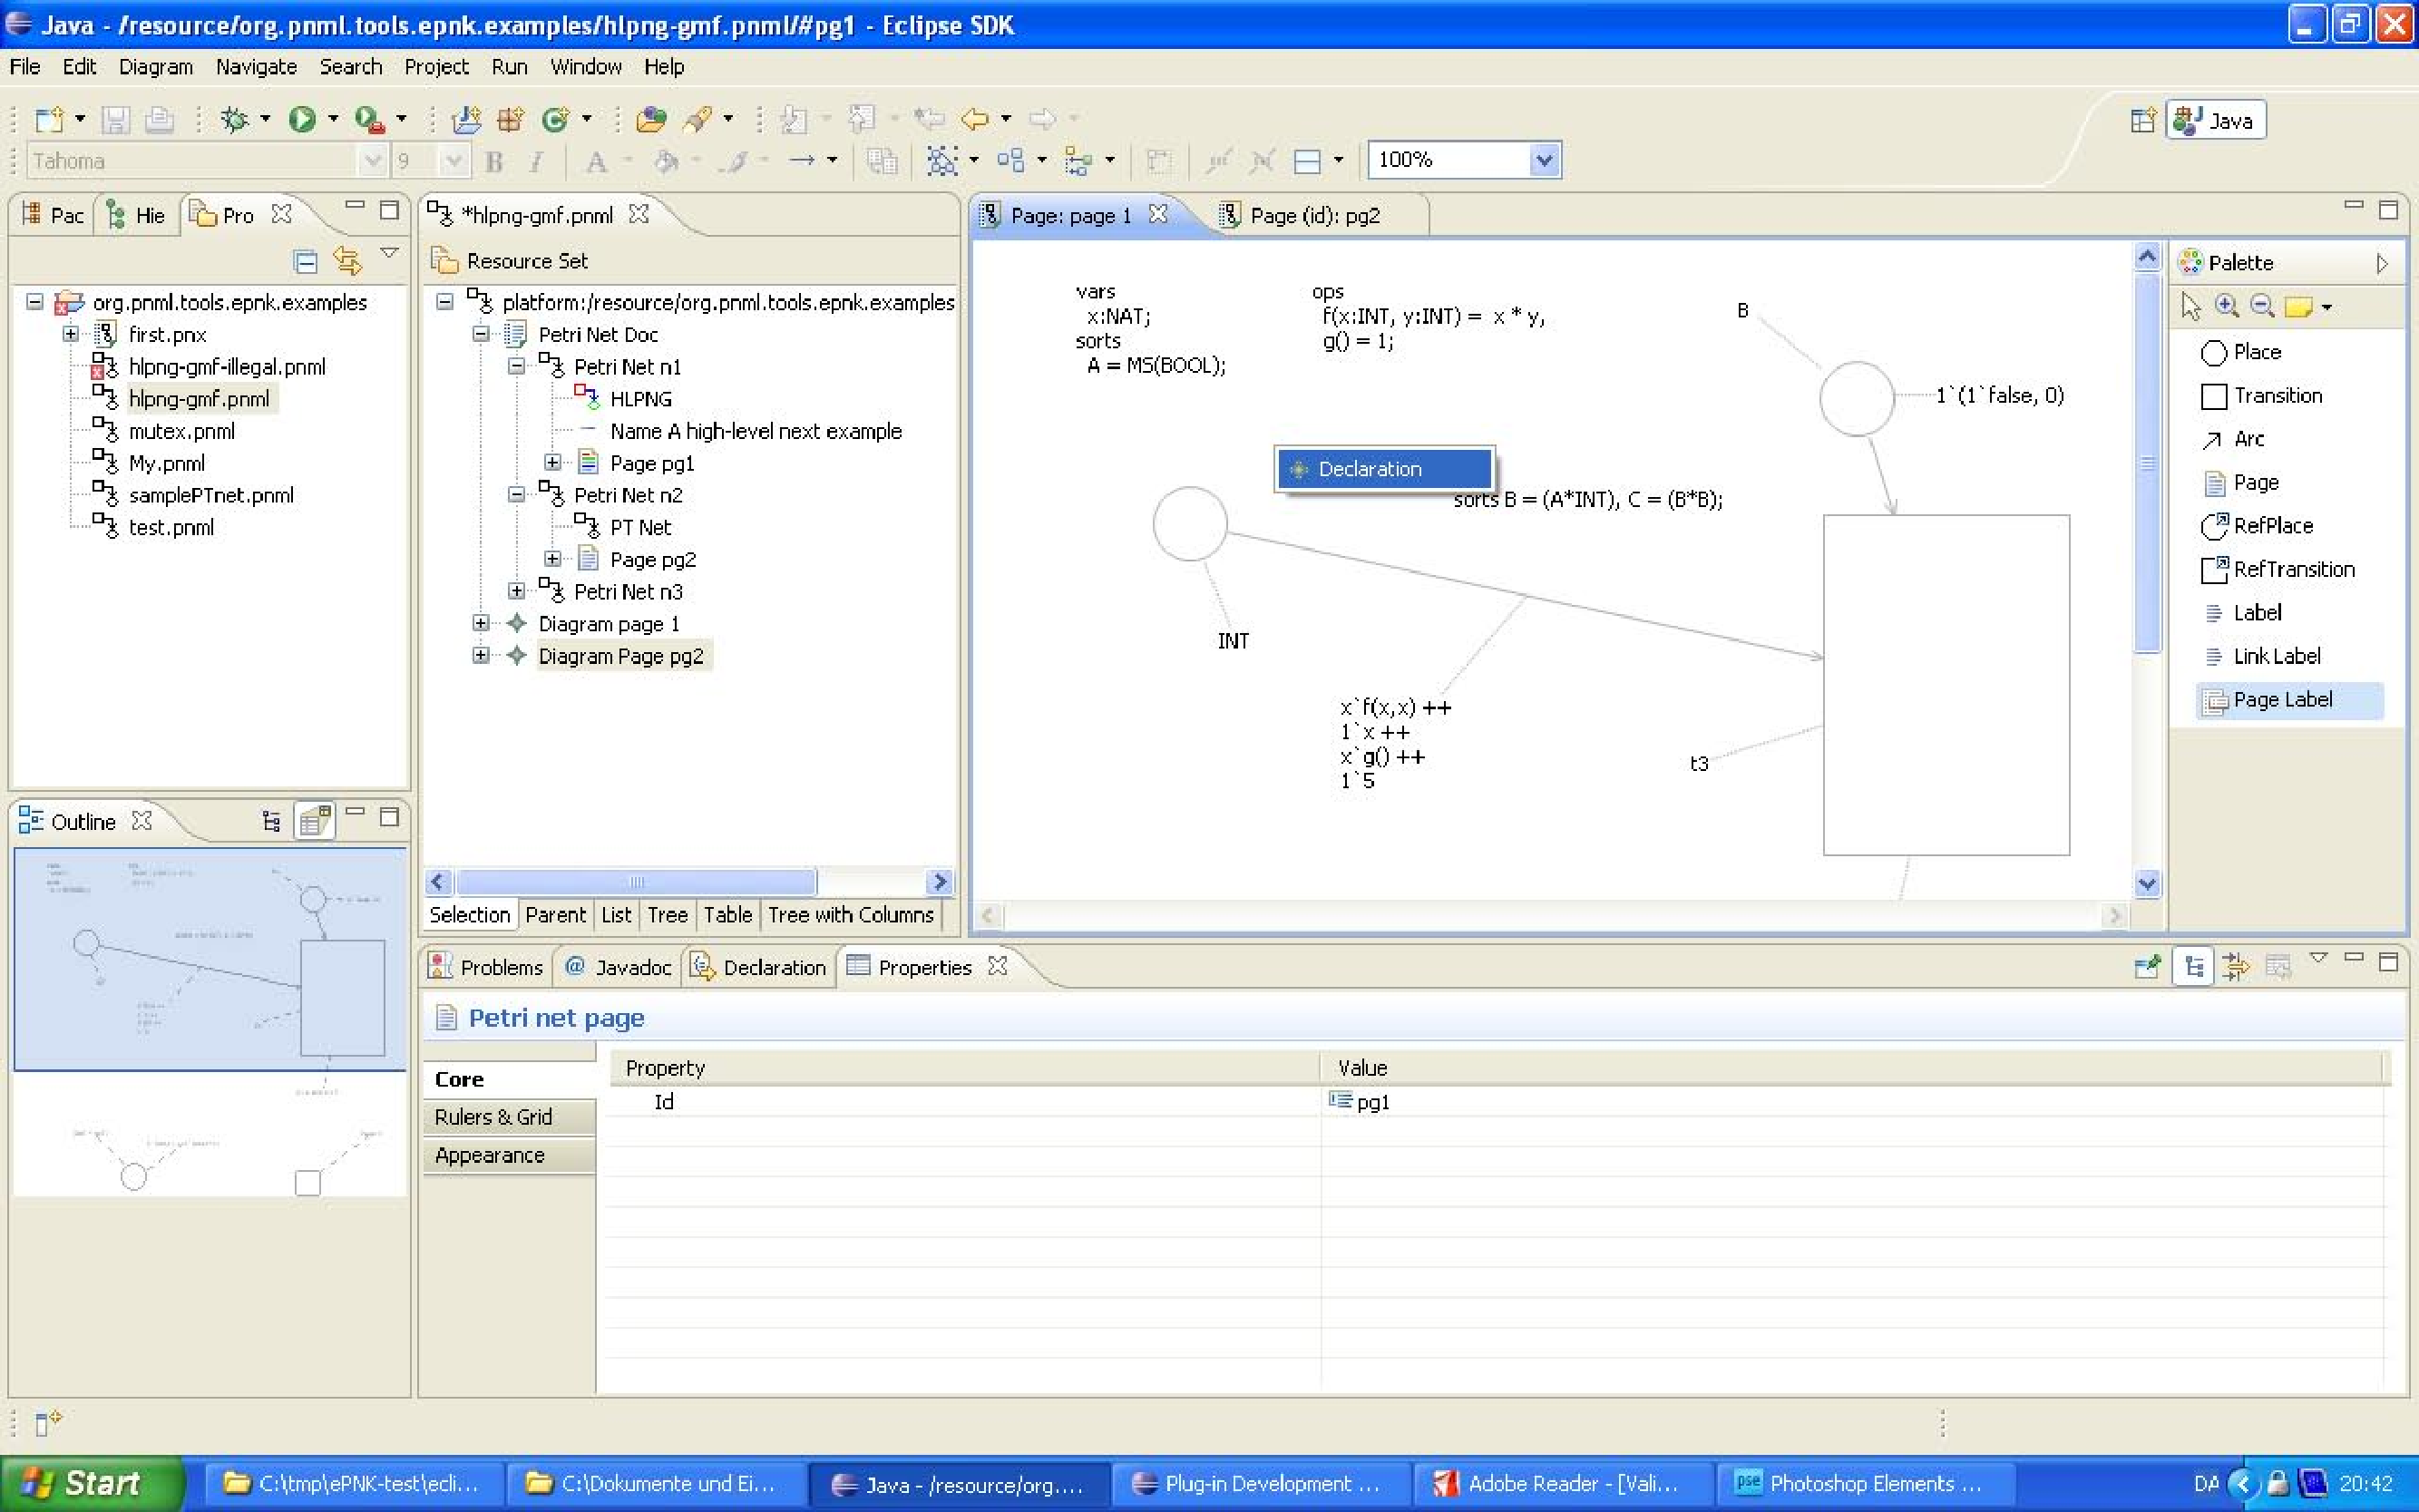
\includegraphics[scale=.25]{CreatePageLabel}}
  \caption{Pop-up menu during page label creation}
  \label{fig:pagelabel-creation}
\end{figure}

The process for creating a label and attaching it to an object is slightly
different. First you must create the label. This new label, however, will
not be attached to any object yet, which is indicated by the text
``\verb+<+not connected label\verb+>+''. A not yet connected label can -- and
must -- be connected to some Petri net object (which could also be a
sub-page) by choosing the tool ``Link Label'', clicking on a label, and then without releasing the
mouse button moving it over the object the label should be attached to.
Then, a pop-up menu will be opened showing you the possible kinds of labels
that could still be attached to the chosen object. This is shown in
Figure~\ref{fig:label-connection} for a label that is attached to a place
of a P/T-System.
The possible options are ``Name'' (which is a legal option for any object, but
only if there is no name attached yet) or ``PTMarking 0'', which is the initial marking
for P/T-Systems (where ``0'' is the default value). After the selection,
the label of the chosen type will be attached to the object.
Again, attaching the label can be aborted by pressing ``ESC'' or by
clicking somewhere outside the pop-up menu.

\begin{figure}[hbt!!]
  \centerline{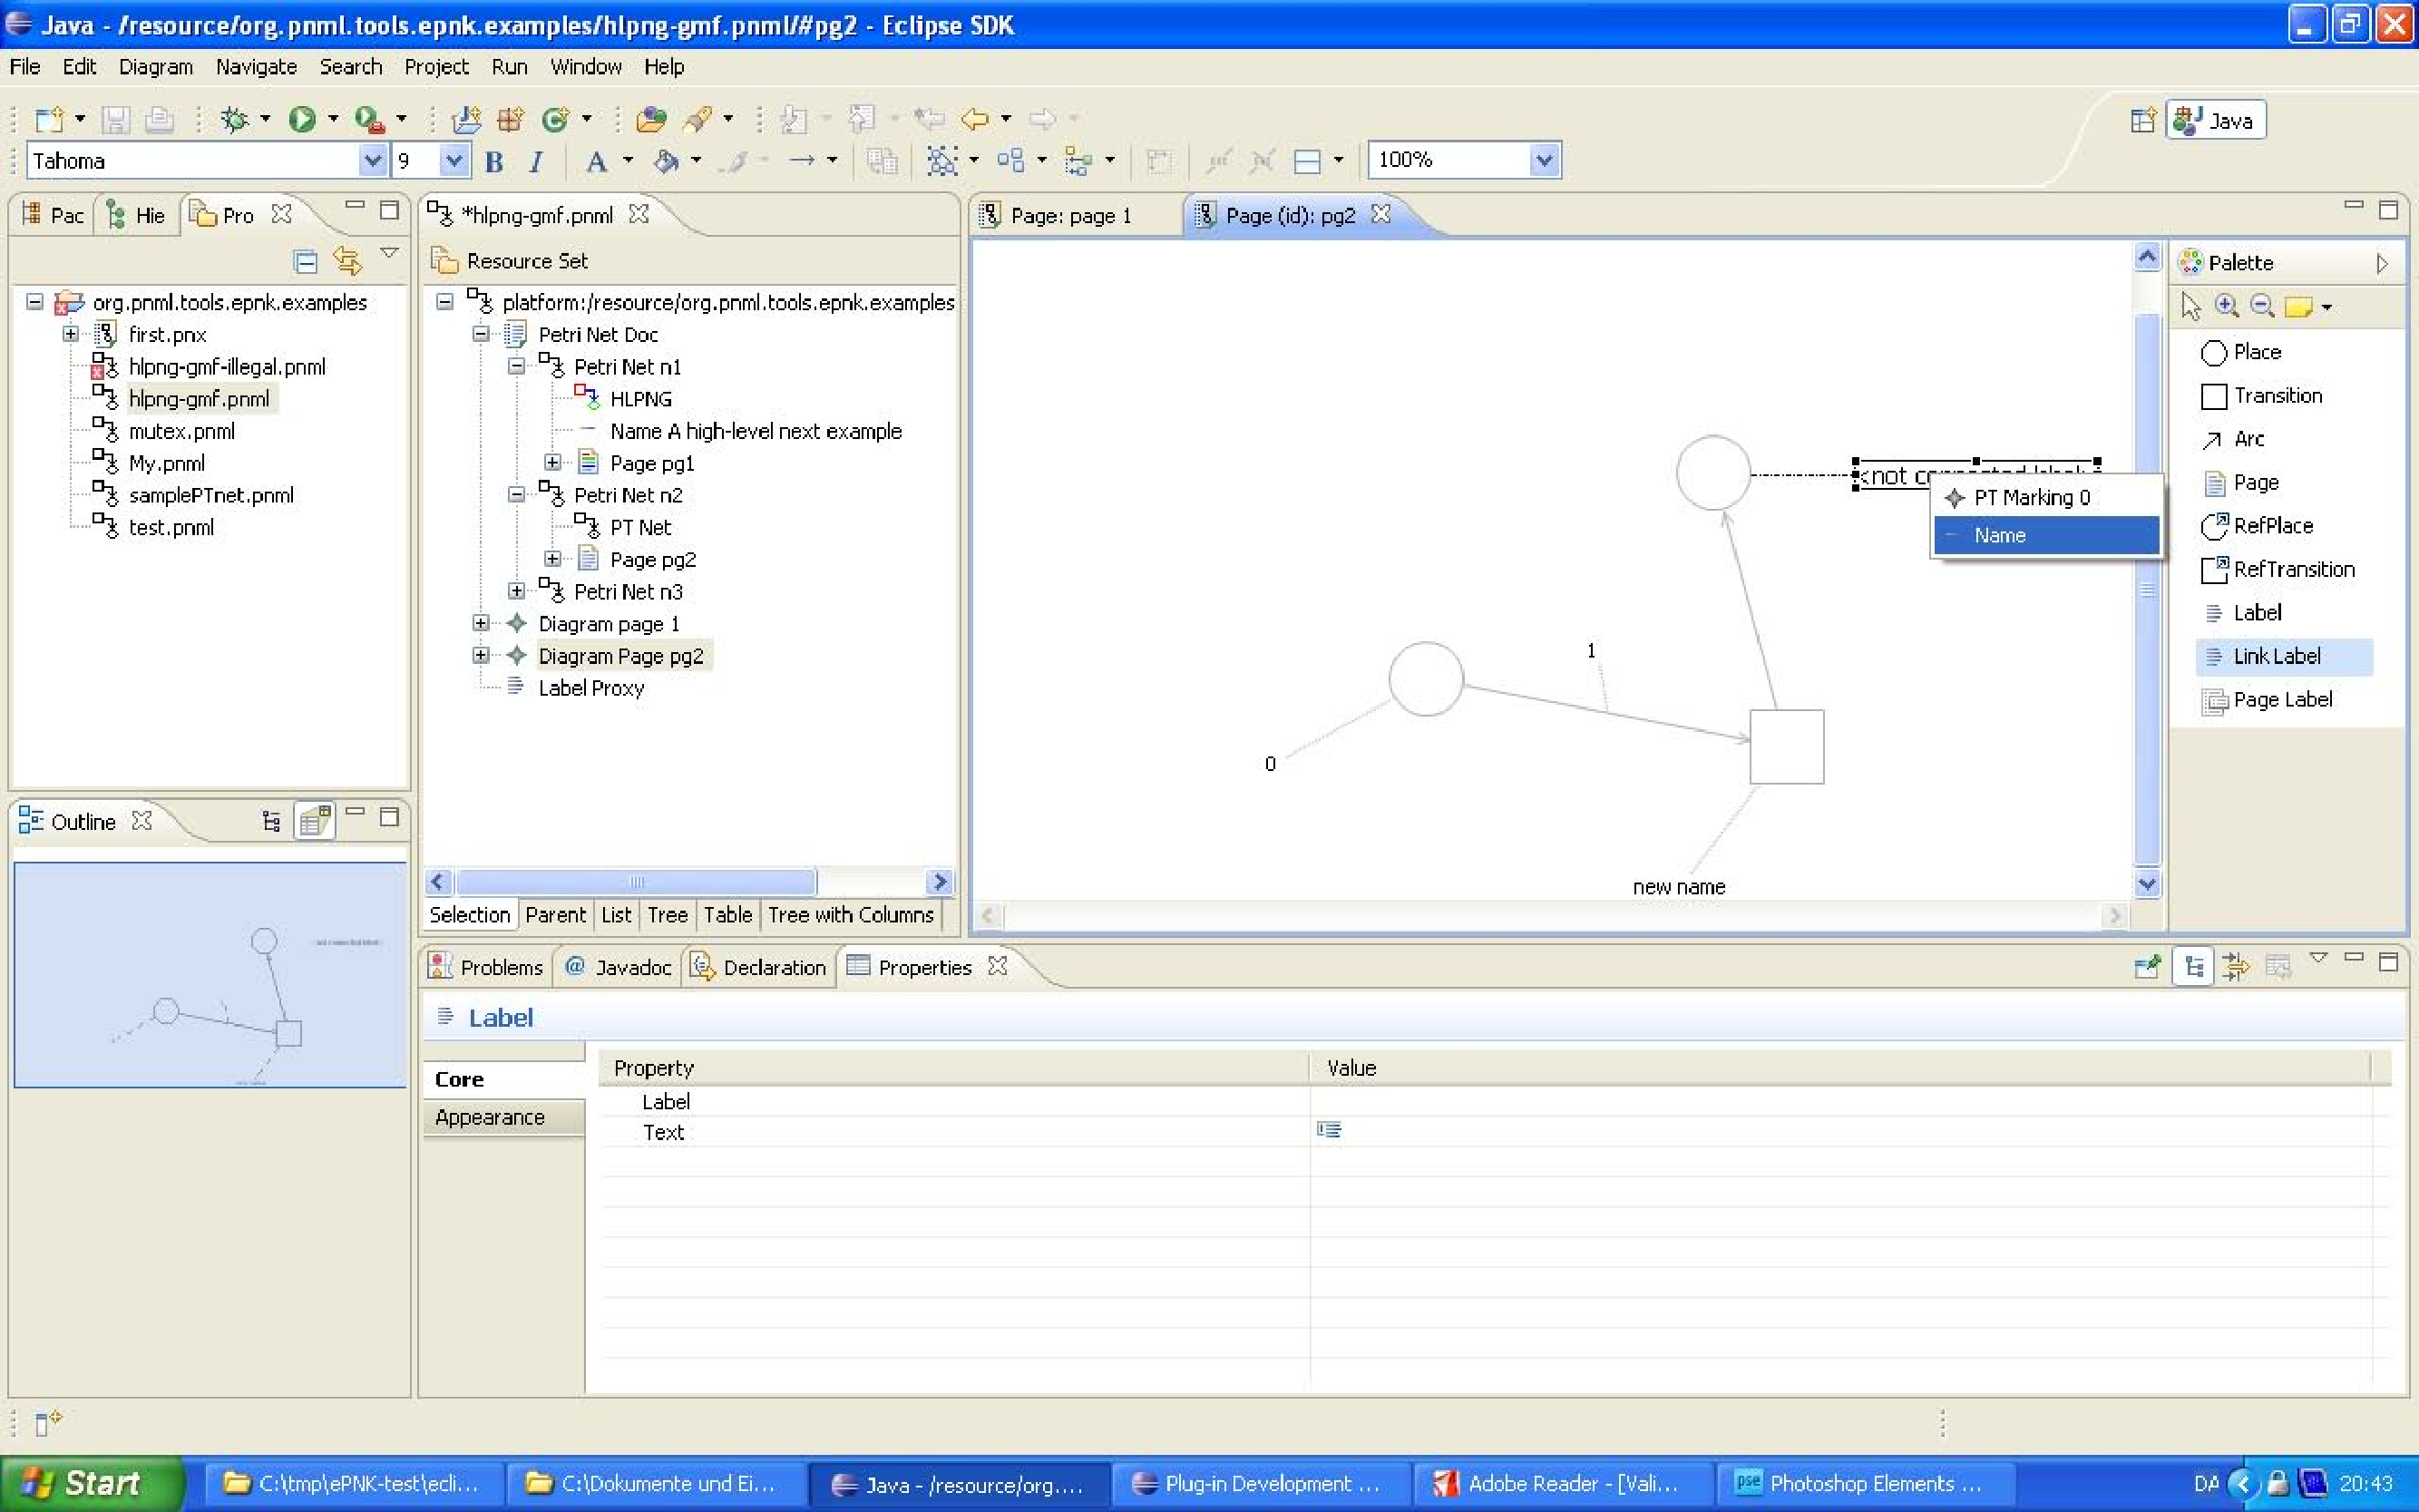
\includegraphics[scale=.25]{AttachLabel}}
  \caption{Pop-up menu during attaching a unconnected label to an object}
  \label{fig:label-connection}
\end{figure}

After the label has been attached to an object, it can be edited ``in place'',
by clicking into it and pressing the ENTER key in the end.  The legal syntax of
the label depends on the Petri net type and which kind of label it is. In
general, when editing labels and page labels there are two different
cases: The first case are \emph{simple labels},%
  \index{Label!Simple|DEF}
which typically are simple
values like ``true'' or ``false'', values like numbers, arbitrary strings,
or IDs (in general, it will be some form of data types). If such a label is
typed in syntactically incorrect, the new value will be rejected, and the
value of that label will be reverted to the value it had before editing. The
other case are \emph{structured labels}.%
  \index{Label!Structured|DEF}
These are, typically, labels with a
complex syntax, as for example the declarations of a high-level net (actually
all labels of high-level nets except for the names are structured). All these
labels will be parsed and checked for syntactical correctness; but the entered
text will be stored in all cases. If the text is syntactically incorrect,
however, the structure is not set and this will very likely result in some
validation%
  \index{ePNK!Validation}
error later (see Sect.~\ref{subsec:validation}). So this error needs to be
fixed, by editing the label again.  In case of such an error, the label will be marked
with a warning symbol (and when the mouse is moved over the warning symbol,
the tool tip will indicate that the label could not be parsed). If, for example,
we delete the comma that separates the two sort declarations in the label
``sorts B = (A*INT), C = (B*B);'' the label will be decorated with a warning
symbol. Upon validation, a validation error message will be given and later shown in the problems view.


The documentation of the legal syntax of these type specific labels, in
particular the one of the structural labels, is part of the documentation
of the Petri net type definition. For the types deployed together with the
ePNK, this information can be found in Sect.~\ref{sec:petrinettypes}.

Note that labels, in principle\footnote
 {That is, if the legal syntax of a specific Petri net type does allow it.}%
, can have line-breaks.  Since pressing the ENTER button will finish the
editing of a label, however, a line-break is inserted to a label by
pressing CNTRL-ENTER while editing the label.

Some Petri net types have quite many labels, and it is quite tedious to
create and link all these labels to a Petri net object. Therefore, the
graphical editor of the ePNK has a context menu when one of its objects
is selected, which will create and attach all missing default labels of that
object (and arrange them equally distributed around the object). The menu
pops up, when the right mouse button is pressed on the element; then select
``ePNK''$\rightarrow$``Add default labels''.%
  \index{ePNK!Add default labels@{Add default labels (menu)}|DEF}
  \index{Label|)}

\subsection{Attributes}
\label{subsec:attributes}

\index{Attribute|(DEF}
As discussed earlier, some ``labels'' of a Petri net object are not
supposed to be represented as graphical annotations of a Petri net object.
These are called \emph{attributes}.  Figure~\ref{fig:signal-net-attributes}
shows an example of a Petri net which uses attributes for some objects. It
is a signal-event net (SE-net)%
  \index{SE-nets}
\cite{StHa97}, which will be used later in the
Developers' Guide of this manual as an example of how to define new Petri net
types for the ePNK\footnote
  {The reason we need to resort to SE-nets here is that all the Petri net types
   that are defined in ISO/IEC~15909-2 use annotations only}. 

\begin{figure}[hbt!!]
  \centerline{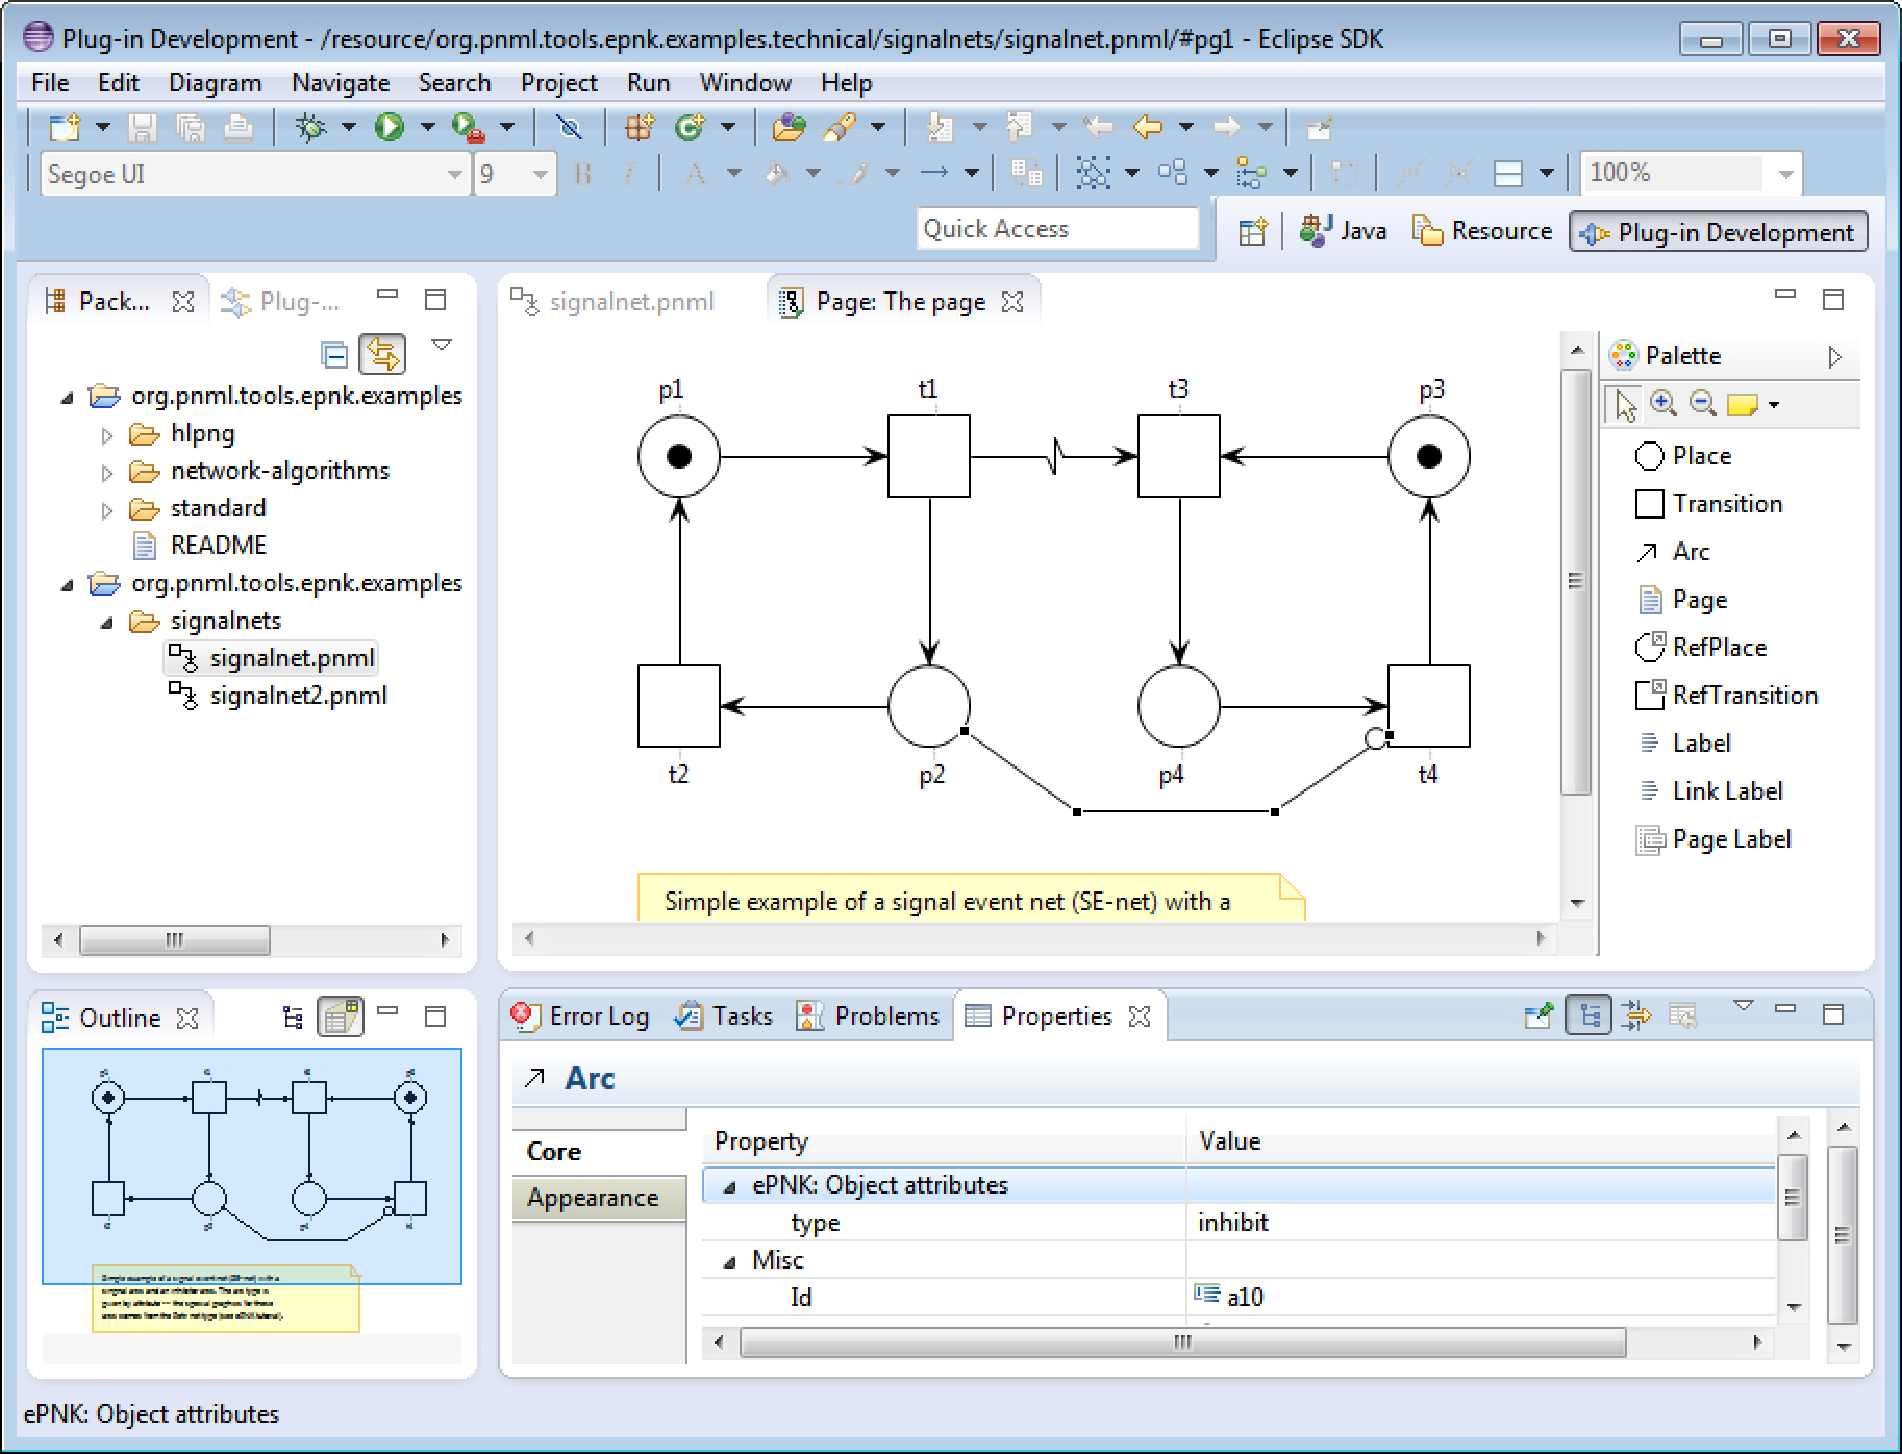
\includegraphics[scale=.38]{signalnet-attributes}}
  \caption{A Signal/Event net open in the graphical editor}
  \label{fig:signal-net-attributes}
\end{figure}

In this example, arcs have an arc type. If the arc type is not set, it is
considered to be a normal arc. The arc that is selected in
Fig.~\ref{fig:signal-net-attributes}, is of type ``inhibit'', i.\,e.\ it
represents an inhibitor arc. The value of the attribute is visible in
the properties view, and can also be changed there. In this example,
the arc is graphically shown as a lollipop -- which comes from the
implementation of that Petri net type, which implements a dedicated
graphical representation for these kind of arcs. Another
example is the signal arc (the one with the ``flash'' decoration), which is an
arc of type ``signal''. For this net type, we have chosen the marking to be an
attribute; therefore, the marking is not shown as a label. It can only be
changed by selecting the respective place, and then changing the
respective attribute in the properties view. In this net type, the marking
is indicated with a special graphics for the place (as black tokens).

As mentioned before, the value of an attribute can be changed by selecting the
respective object and then changing the value in the properties view.
Depending on the type of the attribute, this can be done by either typing
some text into the value column for that attribute or by a drop down menu
(if there are only finitely many possible values). If you want to reset
a value to the default value (the default is that the value is not set at all),
you can right-click into the property column of that property in the properties
view and then select ``Restore default value''.%
  \index{Attribute|)}

\subsection{Pages}
\label{subsec:sub-pages}
\index{Page|(DEF}

The graphical editor also allows you to create other pages on the
page it is showing. In order to avoid confusion, we call such
a page a \emph{sub-page}.%
  \index{Sub-page|DEF}
Creating a sub-page
can be done with the ``Page'' tool, in the very same way in which
places or transitions are created on a page. In the graphical editor,
a sub-page is graphically represented as a rounded rectangle. 

It is possible to open a graphical editor on a sub-page from the
graphical editor via a pop-up menu on the right mouse button: ``ePNK''
$\rightarrow$ ``Start GMF Editor on Page'' (as we have seen it for the tree
editor).
And also here, a double-click on the page in the graphical editor is
a shortcut for opening a graphical editor on this page.
Therefore, the tree editor is needed only for creating the top-level
pages of the net; all the sub-pages could be created by the
graphical editor. But navigation to sub pages might be a bit easier
and much faster in the tree editor; this is why you would probably want to use
the tree- editor for navigating and opening sub-pages further down in the
tree-hierarchy. It is recommended not to create sub-pages in the tree editor,
since they would not have a position in the graphical editor. Still, it is
possible and the graphical editor would show these pages (as well as other
objects created in the tree editor) in the top-left corner, when it is opened
with the graphical editor for the first time. Then, you could move it to
a better position.

The graphical editor indicates by a special decoration when a sub-page is
open in some graphical editor: a symbol of an open folder.

What is more important about pages is how to deal with their labels. Typically,
all the type-specific labels are represented as \emph{page labels}%
  \index{ePNK!Page label|DEF}
on the respective sub-page.
For HLPNGs, for example, the declarations of a page
are shown as page labels on that sub-page. The name, however, will be shown as a label
attached to that page on the super-page.  Which labels are shown as
labels attached to the sub-page on the super page, and which labels are shown
as page label on the opened sub-page is up to the Petri net type definition.%

Note that some Petri net types, allow labels to be directly defined for the net,
in which case they are \emph{net labels}%
  \index{ePNK!Net label|DEF}%
and not \emph{page labels}. This applies for example for all kinds
of declarations in High-level Petri nets (HLPNGs). Though, we do not recommend
to use them, ISO/IEC 15909-2 mandates tools to support them. The ePNL allows
to add net labels in the tree editor, if needed.

Note that even though, a Petri net can consist of many pages, the net is
considered as a single flat net only. \emph{Reference places}%
  \index{ePNK!Reference place}
and
\emph{reference transitions}%
  \index{ePNK!Reference transition}%
, are conceptually merged with the places and
transitions they refer to. This is what we call \emph{flattening of the net}.%
  \index{Flattening (of a net)|DEF}
In Sect.~\ref{subsubsec:developer:functitions:utilities:convenience} of the
Developers' Guide, we will see that the ePNK provides mechanisms for
accessing the flattened net structure in a uniform way.%
\index{Page|)}


\subsection{Graphical features}
\index{ePNK!graphical features|(DEF}

The graphical editor of the ePNK allows you to make all kinds of changes to
the graphical appearance of the Petri net. The features supported are
the standard features of GMF editors. Figure~\ref{fig:signal-net-graphics}
shows the same net as above again; in order to high-light some GMF features
now, the grid and rulers switched on.

\begin{figure}[hbt!!]
  \centerline{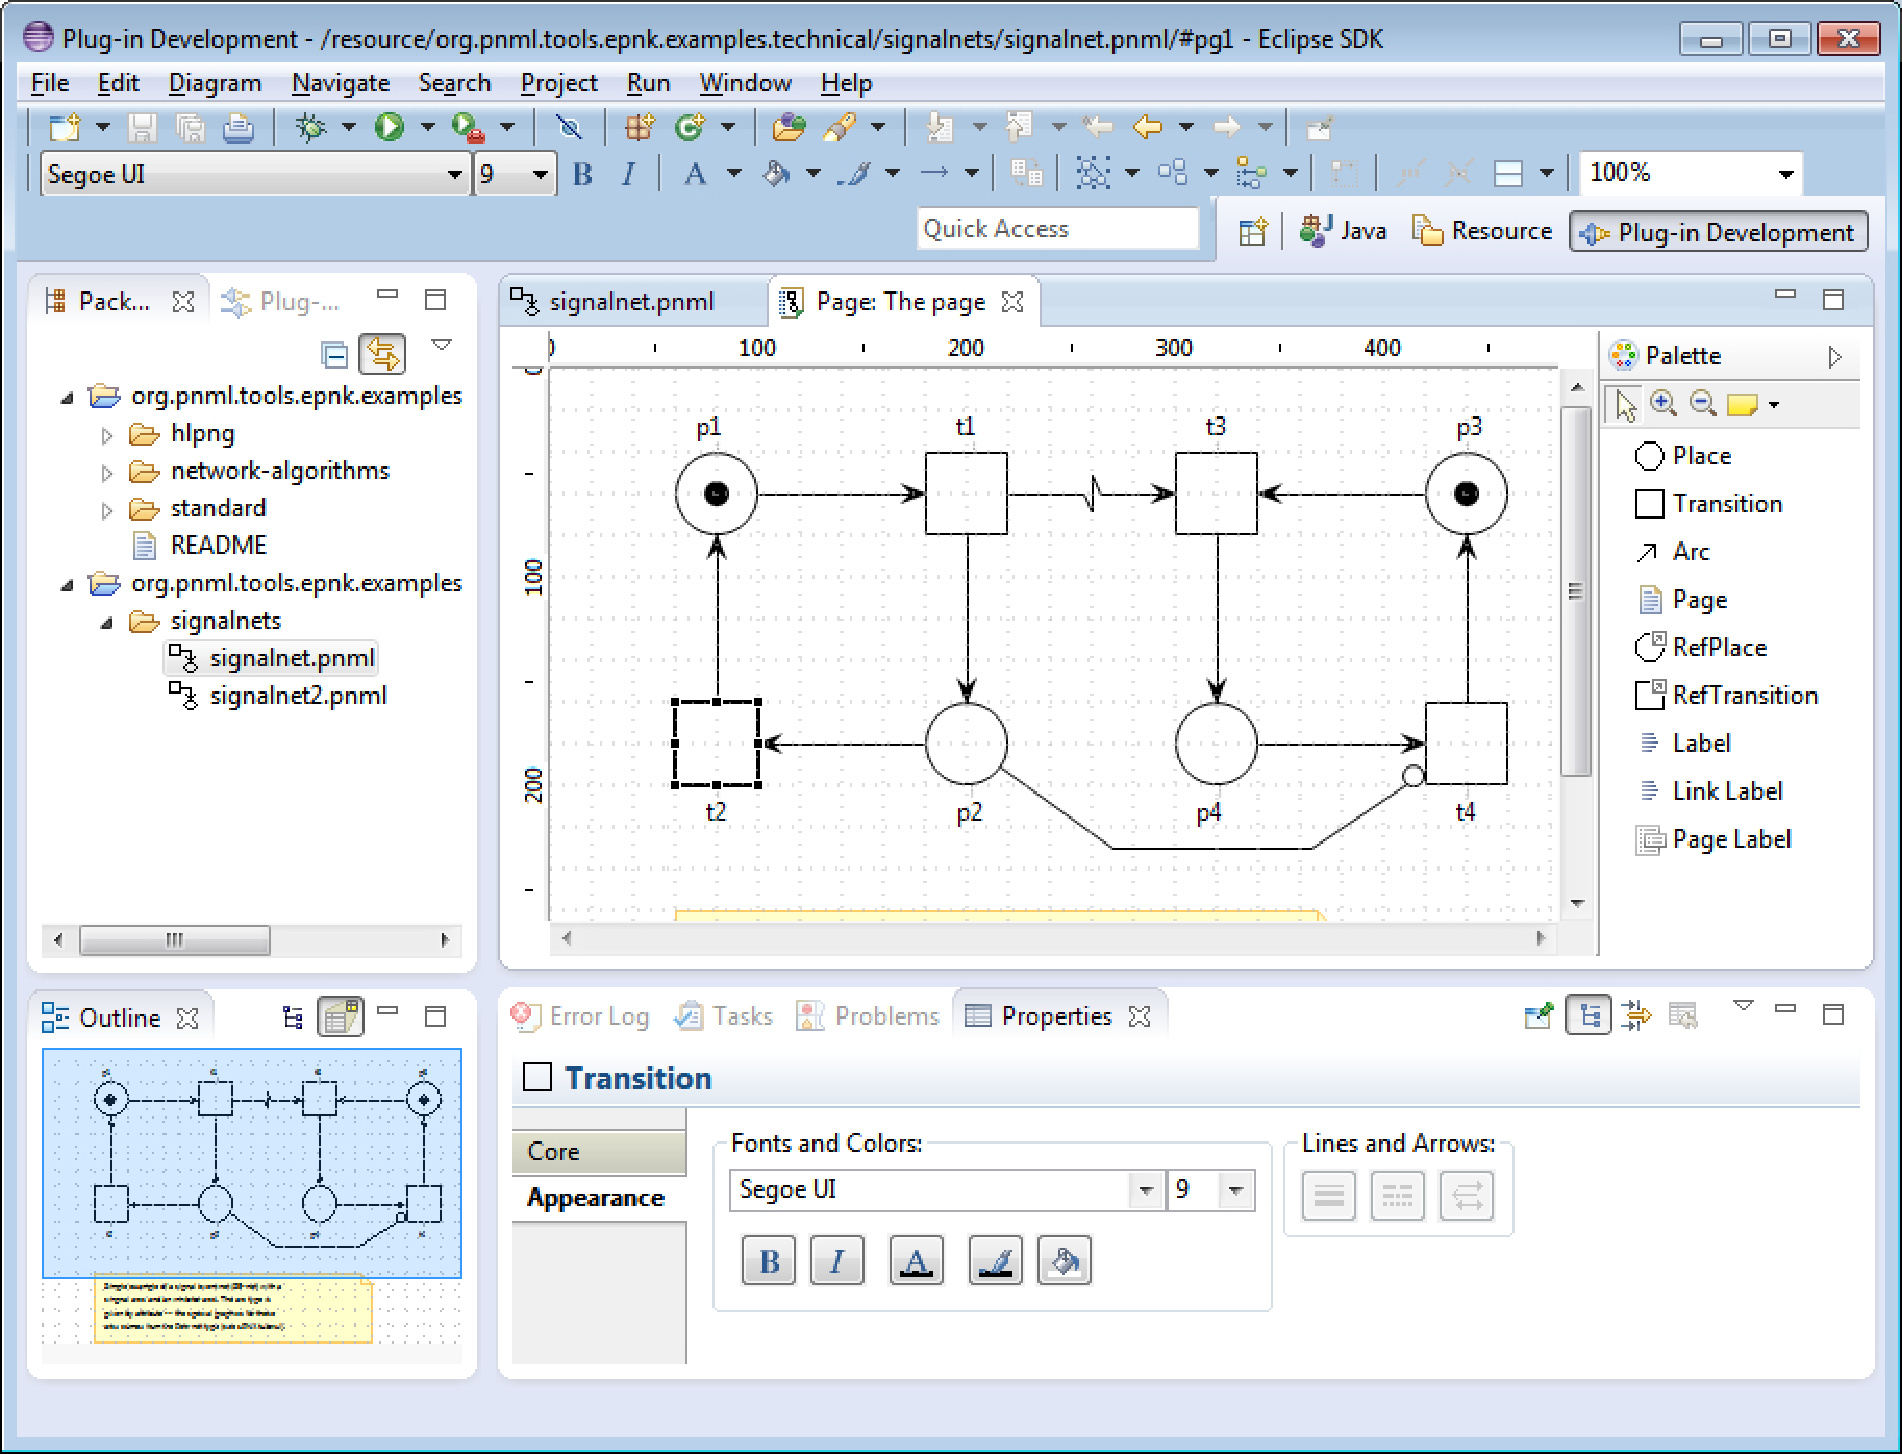
\includegraphics[scale=.38]{signalnet-graphics}}
  \caption{The Signal/Event net again: now with grid and rulers}
  \label{fig:signal-net-graphics}
\end{figure}

Since the graphical features are pretty straightforward, and are similar
to typical graphical editors, we do not explain the details here. The
graphical features can be changed in the properties view, when selecting
the ``Appearance'' section (up to now, the properties view had always
shown the ``Core'' section). Figure~\ref{fig:signal-net-graphics} shows
the graphical features that can be changed, when a node is selected. The
available features vary for the different kinds of objects.

Note that Petri net types can define a special graphical appearance for
some nodes or arcs, which depends on attributes or some other information
of the resp.\ element. In that case, some graphical information selected by
the user might be overruled by the specific graphical information for that
element of the Petri net type. You can see an example of such a specific
graphics in Fig.~\ref{fig:signal-net-graphics}, where signal arcs and
inhibitor arcs are shown in their usual graphical notation. In this example,
however, the specific graphical information does not interfere with the
user graphics. But, if a net type defines that some specific arcs should
be displayed in red colour, for example, this would override the colour chosen
by the user.

The ePNK saves the nets in exactly the graphical representation you
see them before you save the file. But, the exact graphical representation
is saved as a tool specific extension of the ePNK! This means that the
exact graphical representation can be reproduced in the ePNK only.

The ePNK also transfers most of the graphical information to the respective
features of PNML, so that other tools could reproduce almost the same
graphical appearance as you see it in the ePNK. Some features, however,
are not supported by PNML (as for example the size of labels) and some
others are not yet transferred by the ePNK to PNML. In turn, some graphical
features of PNML are not supported by the ePNK editor (e.\,g.\ the alignment
of text in labels).

In Sect.~\ref{subsec:supported-graphical-features}, you will find a complete
list of graphical information that is transferred to PNML elements. Here
is a brief list of graphical information from the graphical ePNK editor
that is \emph{not} transferred to PNML: font styles (bold or italic for labels);
routing and jump link information for arcs. Note that also the comments that
you can place on a page will be lost in other tools, since this is tool specific
information only in the ePNK (comments are not a concept of PNML).

Note that PNML nodes that do not have a size attached to them, will have the
width and height 40pt in the ePNK (which the GMF default). 

Arcs can have \emph{intermediate points} or \emph{bend points}%
  \index{intermediate point|DEF}%
  \index{bend point|DEF}
in the ePNK as well as in the PNML. These intermediate points will be
transferred to the PNML model. But there is some caveat: when a node is moved in
the ePNK editor, the bend points of the attached arcs might also be moved. Due
to some quirk in GMF, these changes are not transferred to the PNML model at
all. If you want to be sure that the intermediate points of the PNML model
corresponds to what you see in the graphical editor of the ePNK, you should
move at least one bend point of each arc attached to the node after you have
moved the node.

Arcs are either drawn as a \emph{polyline} or as a \emph{bezier curves}, which
is defined by the ``Smoothness'' chosen for the respective arc in the ePNK
editor. The ePNK draws an arc as a polyline, if the ``Smoothness'' is%
  \index{Smoothness (of an arc)|DEF}%
  \index{Curved arc|DEF}%
  \index{Polyline arc|DEF}
set to ``None''; for all other choices of ``Smoothness'' (i.\,e.\ ``Normal'',
``Less'', or ``More'') the arc will be drawn as a quadratic bezier curve,
where every second intermediate point is used as a control point as mandated
by ISO/IEC~15909-2. The information on whether an arc should be drawn as a
straight line or as a bezier curve is transferred to the PNML model.
 
\index{Image|(DEF}
The graphical editor of the ePNK also supports the \emph{image} feature of PNML:
Every node can be assigned an image in the PNML model; instead of the 
normal shape of the respective node, the image will be shown. The ePNK
supports JPEG and PNG -- as required by PNML. Actually, the ePNK supports
even more image formats\footnote
  {All image formats supported by the Eclipse SWT {\tt ImageLoader}
   should work: BMP, ICO, JPEG, GIF, PNG and TIFF.}%
. But, since the other formats are not supported by PNML, we recommend
to use the JPEG and PNG format only.

% Right now, the image attribute of a node (in the Fill element of the
% NodeGraphics) can be set in the tree editor only. From version~1.0.1 on, 
The properties view has an image property, in which the path to the image
can be set directly when the resp.\ element is selected in the graphical editor.
The paths should be a relative path to the image, staring from the folder that
contains the PNML document.

Note that, for efficiency reasons, each image is loaded only once -- the first
time it needs to be shown in the graphical editor. If you change an
image file and you want a graphical editor in an already open document to
show the new image, the \emph{image cache}%
  \index{ePNK!Image cache|DEF}
of the open editor must be cleared
explicitly. To this end, right-click on the top-level ``Petri Net Doc''
element in the ePNK tree editor of that document and select
``ePNK$\rightarrow$``Clear Image Cache''.%
  \index{ePNK!Clear image cache|DEF}
  \index{Image|)}%
  \index{ePNK!graphical features|)}%
  \index{ePNK!Graphical editor|)}%

\section{Petri net types} 
\label{sec:petrinettypes}
\index{PNTD|DEF}

In this section, we give an overview of the Petri net types that are
deployed together with the ePNK. In the basic version of the ePNK, these
are \emph{P/T-Systems} (\emph{PTNet})%
  \index{P/T-Systems|DEF}
  \index{ePNK!PTNet|DEF}
and \emph{high-level Petri nets} (\emph{HLPNG}).%
  \index{High-level Petri nets|DEF}
  \index{ePNK!HLPNG|DEF}
Moreover, there is the \emph{empty type} (\emph{Empty}),%
  \index{Empty (net type)|DEF}
which, however, does not contain any concepts in addition to the
PNML core model; therefore, we do not discuss the empty type here. The empty
type was introduced to explicitly indicate, that there are no Petri net type
specific extensions. 

Actually, HLPNGs come in different levels or kinds: ``\emph{dot nets}'',%
  \index{ePNK!Dot net|DEF}
which are a way of representing P/T-Nets as high-level nets; basically, ``dot
nets'' are high-level nets restricted to the sort ``DOT'' and a minimal version of
operators on them; ``\emph{symmetric nets}''%
    \index{ePNK!Symmetric net|DEF}
are a restricted version of
high-level nets that uses  some special finite sorts and a limited set of operations only;
and the full version of high-level nets. The kind of a HLPNG can be
changed by selecting the HLPNG type in the tree editor and by selecting the kind
attribute in the properties view (identified by the respective URI as defined by
ISO/IEC~15909-2).
For a detailed discussion of the legal constructs of the different kinds of HLPNG,
we refer to the discussion of ISO/IEC 15909-2 \cite{HKea09}. Note that, in
contrast to the Petri net type, the kind of a HLPNG can be manually changed anytime, since the kind of HLPNG
concerns the validation only. The PNML syntax is the same.

\subsection{PTNet}
\label{subsec:PTNet}
\index{ePNK!PTNet|(DEF}

We start with explaining the details of \emph{PTNets}. In
Sect.~\ref{subsec:PNTD} we have already seen the additional features of 
PTNets, which are the initial marking for
places and the inscription for arcs. Both labels are simple labels, which
means that it will be checked right after editing a label whether the label is
syntactically correct (see Sect.~\ref{subsec:labels}); if it is not
correct, the value will be reverted to the value it had before.

The marking of a place must be a non-negative integer in any reasonable
representation\footnote
 {For those who want to bother with the technical details, it can be any
  String that would be accepted by the Java {\tt Integer.parseInt()}
  method as a number and that evaluates to a number greater or equal than 0.}%
.  The arc-inscription is similar, just that it must represent a positive 
integer (i.\,e.\ must be a number greater than 0).

Moreover, PTNets have the restriction that arcs may only run from a
place to a transition or from a transition to a place, which will
be enforced in the graphical editor\footnote
  {In the tree editor, illegal arcs can be created, but the respective net
   would not pass validation.}%
. Actually, the constraint is slightly more complicated due to
reference nodes: We can connect place-like nodes (PlaceNodes)
with transition-like nodes (TransitionNodes) and vice versa;
but semantically, i.\,e.\ when flattening a net (see
Sect.~\ref{subsec:sub-pages}), this amounts to the above condition.%
  \index{ePNK!PTNet|)}

\subsection{HLPNG}
\label{subsec:introHLPNG}
\index{HLPNG|(DEF}

\emph{HLPNGs} are much more involved than P/T-Nets and we cannot explain
them in all details here. For a detailed motivation and full account
on what \emph{HLPNGs} are, we refer to ISO/IEC~15909-2
\cite{ISO-IEC:15909-2-2011,HKea09}. Actually, HLPNG are
conceptually quite close to coloured Petri nets \cite{JeKr09} or
algebraic system nets \cite{KiRe96}.

For HLPNGs, there are the following labels (in addition to names):
\begin{description}
  \item[Declaration] A \emph{declaration}%
       \index{Declaration|DEF}%
is a page label, which is used
     to define \emph{variables}%
       \index{Varialble|DEF}%
, \emph{sorts},%
       \index{Sort|DEF}%
     and \emph{operators}%
         \index{Operator|DEF}%
, which can then be used in the other labels.  Every page can have
     any number of declarations and, within a single declaration,
     different kinds of declarations can be mixed. Note that all
     declarations are global (known in the complete Petri net),
     even though they are attached to a specific page.
     
     Declarations do not need to be contained in a page at all --
     they can be contained directly in the net. We do not recommend
     to make use of that; but ISO/IEC~15909-2 mandates
     this to be possible. So, the ePNK can read nets with declarations
     which are directly contained in the net and such net labels can
     be created in the tree editor of the ePNK, if needed.

  \item[Type] A \emph{type}%
       \index{Type|DEF}
     is a label that is associated with a place.
     Every place must have exactly one type label which denotes
     the sort of the tokens on that place. This sort can be built
     from the predefined sorts of HLPNGs or some user-defined sorts.

  \item[HLMarking] A \emph{marking}%
       \index{Marking|DEF}
     is a label that is attached to a place
     and defines the place's initial marking. The marking is
     represented by a ground-term\footnote
      {A ground-term is a term that does not contain variables.},
     which must denote a multiset over the place's type. Note that this
     label may be omitted, in which case the initial marking is
     considered to be empty. There can be at most one label of this
     kind.

  \item[Condition] A \emph{condition}%
       \index{Condition|DEF}
     is a label that can be attached
     to a transition. The condition is a term of type boolean and
     can contain variables. There can be at most one condition;
     if the condition is missing, it is assumed to be true.

  \item[HLAnnotation] An \emph{arc annotation}%
       \index{Arc annotation (HLPNGs)|DEF}
     is also a term that may
     contain variables. The term must be a multiset term over the
     type of the place to which the arc is attached. Every arc should
     have exactly one arc annotation\footnote
     {Actually, ISO/IEC~15909-2 would allow that this label is
      missing. This does not make much sense though since, in most cases,
      there is no reasonable standard interpretation if the label is
      missing.}.
\end{description} 

All labels of HLPNGs are structural labels (see Sect.~\ref{subsec:labels}),
which means that the user can edit them and leave them syntactically incorrect.
Of course, this will not pass validation; but, it is possible to save
nets with incorrect labels and load them again, so that the labels can
be corrected another time.

PNML does not define or mandate a concrete syntax for declarations and terms.
The concrete syntax for the labels is up to each tool; so it might be different
in different tools. What matters is the abstract syntax. In order to, get
the abstract syntax of a HLPNG net of some net from another tool into the
concrete representation of the ePNK, the ePNK provides a pop-up action,
which converts the abstract syntax into ePNK's concrete syntax. It is
available in the tree editor\footnote
  {Note that you must have installed the ``HLPNG Label Serialisation'' feature
   for this to work.}%
, when a HLPN object is selected ``ePNK''$rightarrow$``Serialise HLPNG
Labels''.%
  \index{HLPNG Label Serialisation|DEF}

ePNK's concrete syntax for HLPNG labels resembles the one of CPN Tools
\cite{JeKr09}, but it is not identical to the one of CPN Tools! Below, we
explain this ePNK's concrete syntax for labels. Before going into the details
of the syntax, we briefly discuss some examples.

The following shows several declarations of variables, sorts and operators.
Each of them could be in a separate declaration label, but they could also be
contained in a single declaration:
\begin{verbatim} 
vars
  x:NAT;
  
sorts
  A = MS(BOOL);
  
ops
  f(x:INT, y:INT) =  x * y,
  g() = 1;
  
sorts B = (A*INT), C = (B*B);    
\end{verbatim}

First, a variable x of built-in sort NAT is defined. Then a user-defined
sort A is defined, which is a multiset over the built-in sort BOOL. Then,
two named operations are defined, f and g. The operation f takes two parameters
of type INT; the operation g does not have parameters. Note that named
operations, basically, are abbreviations and, therefore, do not allow any
recursion (see \cite{HKea09} for details). In the end, two other user-defined
sorts are defined: B is a product of A and the built-in sort INT, and C is a pair over
sort B. Note that also for sort declarations, recursion is not allowed.

The right-hand sides of the sort declarations above give you an idea of the
syntax for sorts already. There are some built-in sort like BOOL, INT, NAT, POS and
DOT. From these, we can built products or multiset sorts.

Here are some examples of terms (using the above declarations):
\begin{verbatim}
 x`f(x,x) ++ 1`x ++  x`g() ++  1`5
 
 1`(dot,1) ++ 1`(dot,1*1)
 
 x > 1 and x < 5 
\end{verbatim}
The first is a multiset term over the sort INT, which could be used in
arc inscriptions (if the attached place is of type INT). The second is
a ground term over the product of built-in sort DOT with INT, where DOT is
a sort that represents a type with a single element dot. The last term
is a term of sort BOOL, which could be used as a condition.

The precise syntax is defined by the following grammar (that actually is
a simplified version of the grammar that was used for generating the parser).
The terminals ID, INT, NAT, STRING in this grammar represent legal identifiers
and legal representations of integer numbers, non-negative integer numbers
and string constants.

Listing~\ref{lst:grammar1} shows the part of the grammar for declarations.
\begin{figure}[htbp!]
\lstinputlisting[label=lst:grammar1,stringstyle=\normalsize,%
caption={Grammar for declarations}]%
  {HLPNGInscriptionLanguage.xtext}
\end{figure} 
%
Listing~\ref{lst:grammar2} shows the part of the grammar for terms.
\begin{figure}[htbp!]
\lstinputlisting[label=lst:grammar2,stringstyle=\normalsize,%
caption={Grammar for terms}]%
  {HLPNGInscriptionLanguage2.xtext}
\end{figure}
Note that we have simplified the grammar for making it more readable. The
simplification, however, makes the grammar ambiguous (i.\,e.\ some texts could be
parsed in two or more different ways). The ambiguities can be resolved again by
assigning a binding priority to the different operators -- moreover all operators are left-associative.
Each line in the declaration of BinOp represents operators on the same
level of priority, where the first line has the least binding-power and
the last the highest. The unary operators (actually there is only one) have the
highest binding power of all. Note that there are also some operators like the
cardinality, which use circumfix notation: if m is some multiset  \verb+|m|+
denotes the cardinality of that multiset. This operator has the same binding
power as parentheses.

Listings~\ref{lst:grammar3} and~\ref{lst:grammar4} show the part of the
grammar for built-in sorts and constants.
\begin{figure}[htbp!]
\lstinputlisting[label=lst:grammar3,stringstyle=\normalsize,%
caption={Grammar for sorts and constants (1)}]%
  {HLPNGInscriptionLanguage3.xtext}
\end{figure} 
%
\begin{figure}[htbp!]
\lstinputlisting[label=lst:grammar4,stringstyle=\normalsize,%
caption={Grammar for sorts and constants (2)}]%
  {HLPNGInscriptionLanguage4.xtext}
\end{figure} 
Note that every number constant will implicitly be assigned the tightest fitting
sort: INT, NAT, or POS. If a positive integer, say 5 should have the type
INT instead, this can be expressed by 5:INT, which works like a type cast in
object-oriented programming languages.

In addition to these syntactical constraints, the terms must also be correctly
typed, which we do not discuss here in detail. 

For HLPNGs, there are many constraints. Like for PTNets, arcs may only
run from places to transitions or from transitions to places. All of the
other additional constraints concern the correctness of the labels of
HLPNGs. The following list gives an overview:
\begin{enumerate}
  \item Every place must have a correct type (a correct sort in the context of
        the defined sorts of the net).
  \item Every declaration must be syntactically correct and correctly typed.
  \item Every declaration must properly resolve (must not be recursive and all
        symbols it refers to must be defined).
  \item Every term (in markings, arc annotations, and conditions) must
        be syntactically correct and correctly typed.
  \item The marking of a place must be a ground term and must be
        a multiset over the sort of the place.
  \item The arc annotation must be a term that is a multiset over the
        attached place's sort.
  \item Every condition must be a term of sort BOOL.
  \item Every declaration should have a distinct name (actually, this causes a
        warning only since this is a condition on concrete syntax, which is not
        part of PNML).
  \item The parameters of every operation declaration should have distinct names
        (actually, this causes a warning only since this is a condition
        on concrete syntax, which is not part of PNML). 
\end{enumerate}

As mentioned earlier, PNML and ISO/IEC~15909-2 do not define a concrete
(textual) syntax for declarations and terms. The syntax defined here is a syntax
specific to the ePNK. In principle, a PNML document with a high-level Petri net in
it could leave all the textual parts of the labels empty. In that case,
the most important structure and content of these labels would not be
visible in the graphical editor at all. The user would not see and would not
be able to edit the labels textually. In order to convert this structural
information into some text that can be edited by the user in the ePNK, a
simple extension to the ePNK is deployed as a separate feature called ``HLPNG
Label Serialisation''. % It is recommended to install this feature.
%
If you have the ``HLPNG Label Serialisation'' feature installed, you can
serialize all structured labels to the textual syntax of the ePNK. To this
end, right-click on the respective HLPN element (the Petri net) in the
tree editor; then select ``ePNK''$\rightarrow$''Serialise HLPNG Labels''.%
  \index{HLPNG Label Serialisation|DEF}%
  \label{sec:user:hlpng:label-serialisation}%
  \index{HLPNG|)}%
Then, you will be able to see and edit the labels in the syntax that we
have discussed above (independently from which editor the PNML file came from).

\subsection{Other types}

Note that there are some other Petri net types coming with the ePNK, if
if you have the ePNK tutorial installed.  Most notably, there are
\emph{Signal/Event-systems} (\emph{SE-Nets})%
  \index{Signal/Event-systems}
  \index{SE-nets}%
, which we will use as an example later in the Developers' Guide (see
Chapt.~\ref{chap:developers-guide}). Moreover, there is a technical
Petri net type where pages and arcs are equipped with comments, and
arcs can have different types. This type is called \emph{ArcTypes}, but
mainly serves as a tutorial for using attributes, and for equipping
a net with graphical extensions.

If you have the ECNO extensions installed, you have so-called ECNO nets,
which allow to model the life-cycle of elements in the so-called \emph{Event
Coordination Notation}. These are a story of their own \cite{Kin14a} and are not
discussed here.

\section{Functions and Applications}
\label{sec:users-guide:applications}
  \index{ePNK!Function|(DEF}%
  \index{ePNK!Application|(DEF}%
  
The ePNK in its basic version does not come with much functionality for
analysing, simulating and verifying Petri nets. Its main purpose, is
to provide a graphical editor for Petri nets and PNML Documents, and
to provide an infrastructure so that new Petri net types and new functions
and applications for Petri nets can be plugged in. By and by, some functions
have been developed that are now deployed together with the ePNK. And there
are some applications of the ePNK, which are projects in their own right -- for
example the ECNO project, which generates code for so-called ECNO nets
\cite{Kin12b}. We hope, that over time, more functions and applications
of other ePNK developers will be deployed together with the ePNK.

In this section, we explain some of the basic functions and applications
that are deployed together with the ePNK. In these examples, we will
also explain the \emph{ePNK applications view},%
  \index{ePNK!Applications view}
which is used as a
general user interface for the end user to control ePNK applications. 
Later, in the Developers' Guide in Chapt.~\ref{chap:developers-guide}, we
explain how you can contribute your own functions and applications to the ePNK.

Generally, the ePNK distinguishes \emph{functions} and \emph{applications}.
A \emph{function}
is something, which is initiated on some Petri net, possibly asking the user for
some extra input, then does some computation, and when the computation is
finished, provides some output to the user in form of some dialog. After that,
the function and its result are gone. One example of such a function is the
verification of some CTL formula for some Petri net by a model checker, which
is discussed in Sect.~\ref{subsec:user:model-checker}. In particular, the
model checker does not show or visualize any result in the Petri net itself.
Also an \emph{application}
is initiated on some net. In contrast to a function, the application
has a longer live-time, it shows some feedback to the user on top of the
Petri net in the graphical editor, and also provides means for the user
to interact with the application. An example of such an application is a 
simulator for high-level Petri nets, which is discussed in
Sect.~\ref{subsec:user:hlpng-simulator}. This simulator shows
graphically which transitions are currently enabled, and, by clicking
on them, the user can determine which transition should fire next.%
  \index{ePNK!Function|)}%
  \index{ePNK!Application|)}%

\subsection{A simple model checker for EN-systems}
\label{subsec:user:model-checker}
\index{Model checker|(}

In this section, we briefly discuss how to use the \emph{model checker}, which
can be initiated on P/T-nets. Note that even though this model checker
is initiated on P/T-nets, the model checker interprets the net as
an Elementary Net System (EN-systems) \cite{Thi87,Roz87}, which means
that at any time on any place, there can be at most one token.
A transition that would add another token to a place, would not be
able to fire -- and all arc-inscriptions are ignored.

Figure~\ref{fig:user:multi-agent} shows a P/T-net which consists
of several pages. Page {\sf pg0} (not visible) contains
a single place {\sf semaphor} with one initial token, and pages
{\sf pg1}, {\sf pg2}, and {\sf pg3} model three agents with the same
life-cycle, which is shown in the graphical editor in
Fig.~\ref{fig:user:multi-agent}.
%
\begin{figure}[hbt!!]
  \centerline{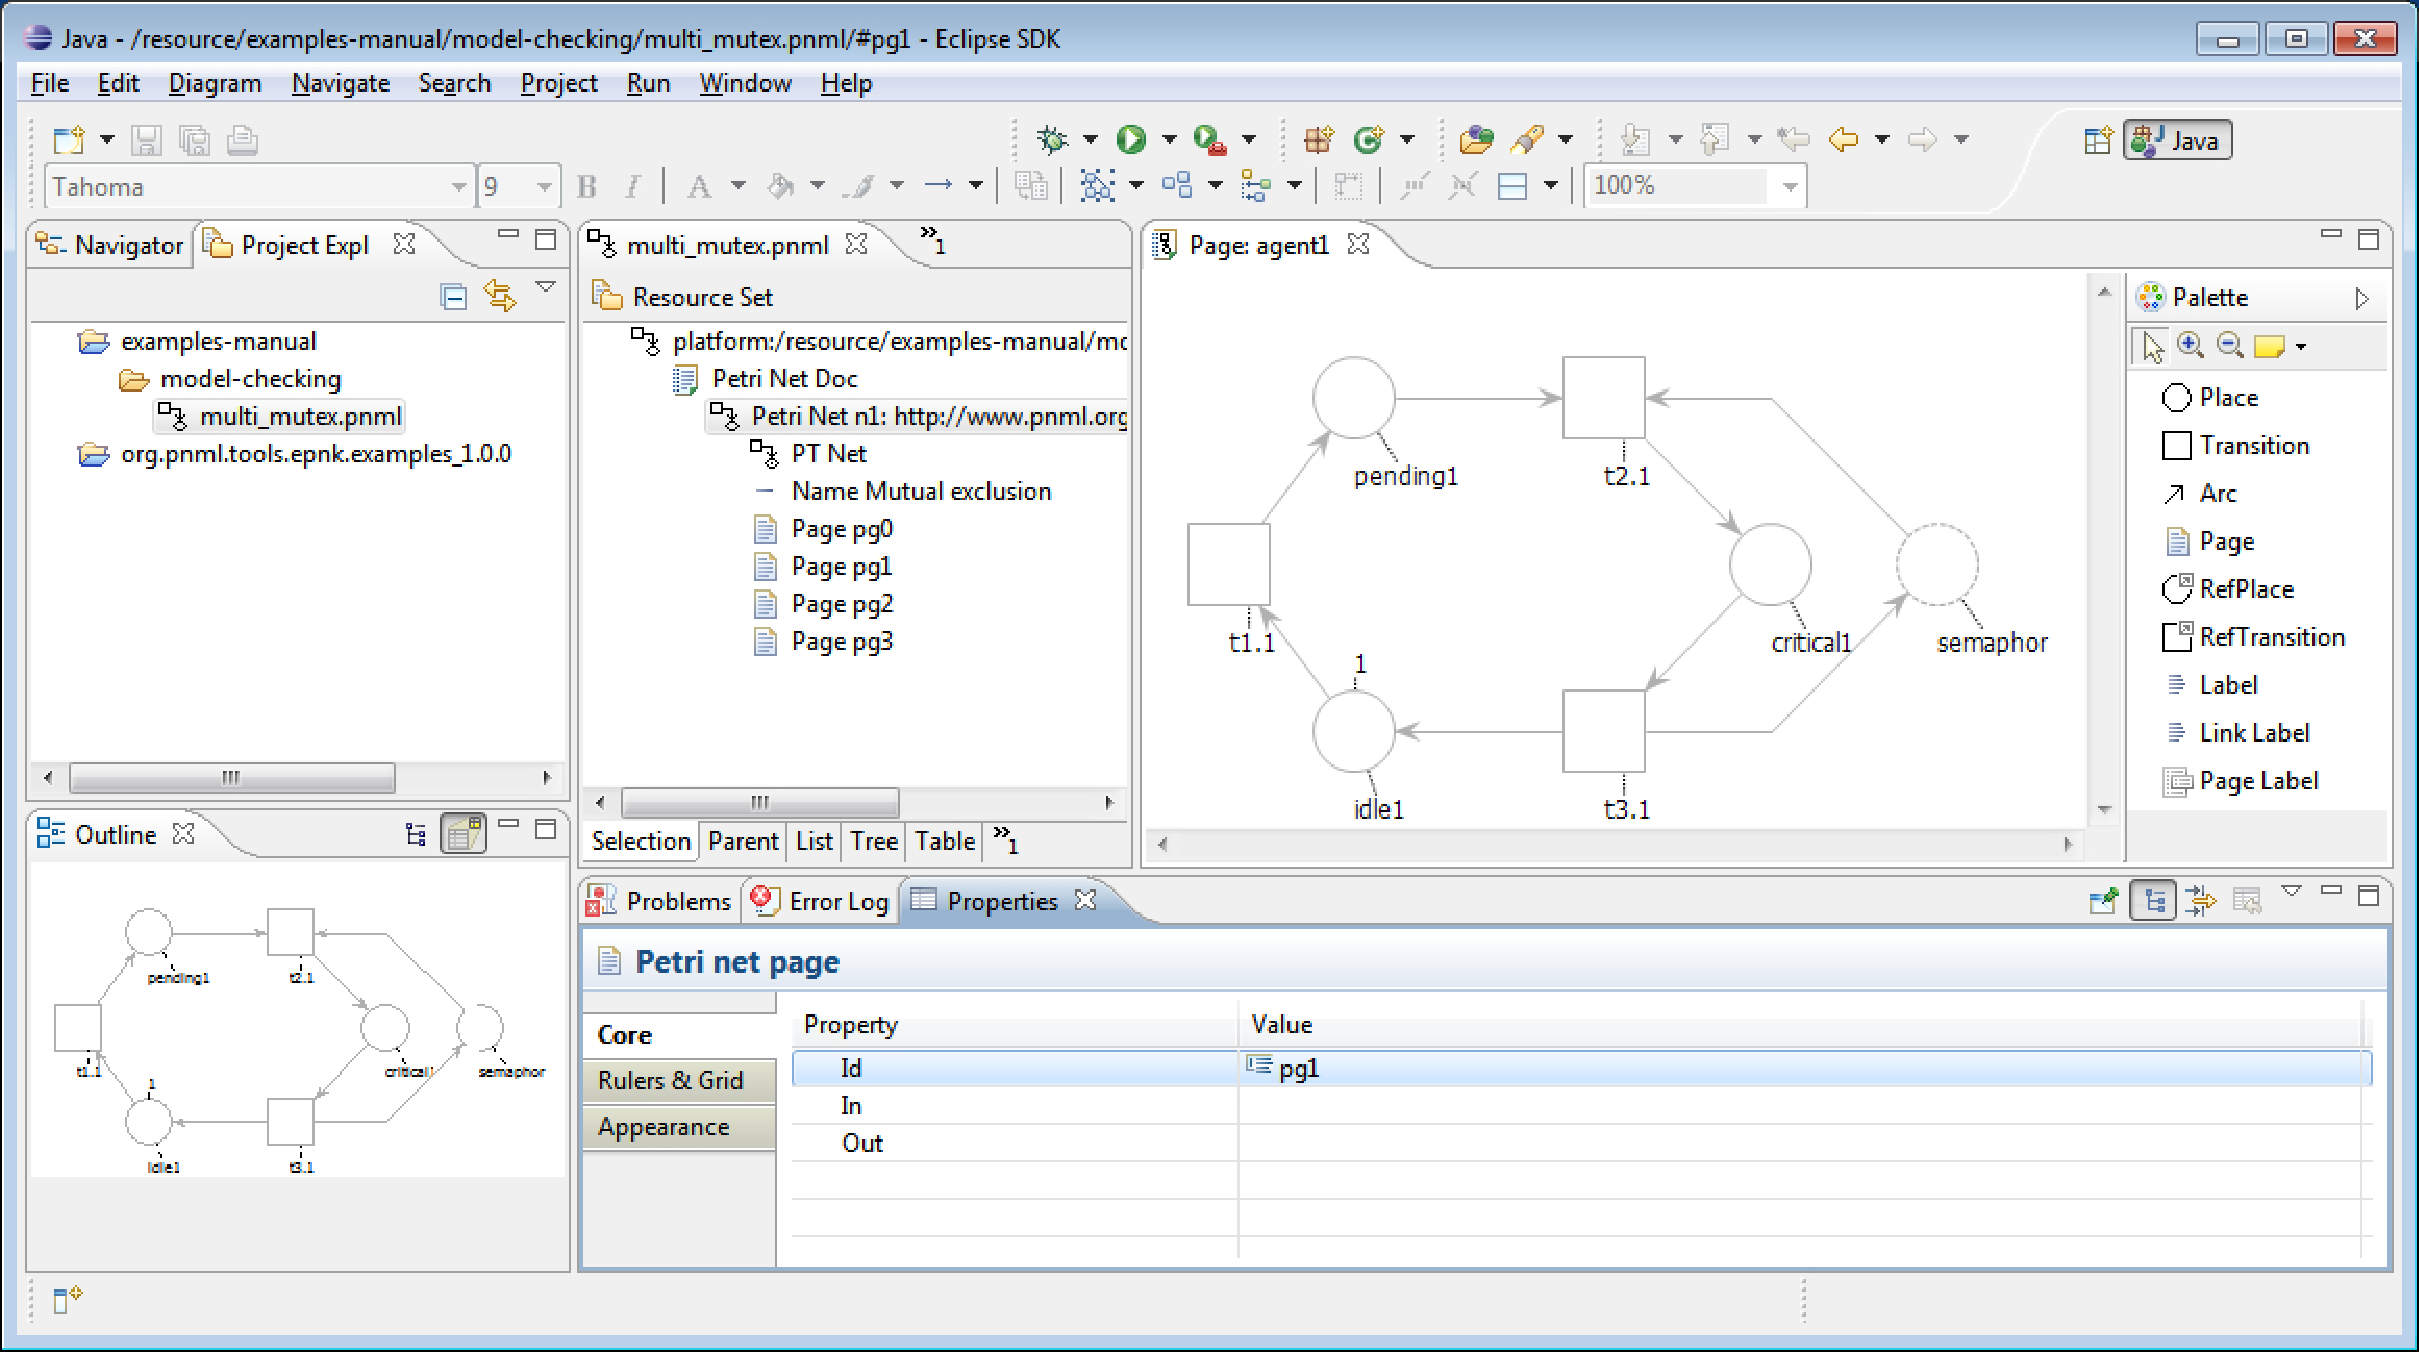
\includegraphics[scale=.30]{MultiAgents}}
  \caption{Mutex example with multiple agents}
  \label{fig:user:multi-agent}
\end{figure}
%
The three agents are competing for the semaphor in order to
access their critical section {\sf criticalx}. Actually, this
net was automatically generated by a wizard for creating a net
with any number of agents. This wizard can be initiated by
``File''$\rightarrow$``New''$\rightarrow$''Other...'' and
then selecting ``Multi-agent Mutex Net Wizard'' from the 
category ``ePNK''. 

The model checker on this net can be initiated by right-clicking
on the Petri net element in the tree editor and then selecting 
``ePNK''$\rightarrow$``Model checker''. Then, a dialog like the
one in Fig.~\ref{fig:user:modelchecker-dialog} pops up, where
two CTL formula, which make sense in any system, are provided
as a default input to the model checker:  
\begin{verbatim}
AG EX true, EG EX true # deadlock free, infinite path
\end{verbatim}
As indicated by the comments behind the hash symbols, these two
formula will check whether the system is deadlock free and whether
there is at least one infinite path.
%
\begin{figure}[hbt!!]
  \centerline{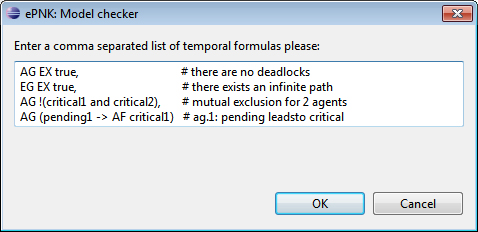
\includegraphics[scale=.40]{ModelCheckingDialog.jpg}}
  \caption{Model checking dialog: Input of formulas}
  \label{fig:user:modelchecker-dialog}
\end{figure}
%
You can of course enter some other formulas, which can use place
names in order to formulate some more specific properties like:
\begin{verbatim}
AG !(critical1 and critical2) # mutual exclusion for 2 agents
AG (pending1 -> AF critical1) # ag.1: pending leadsto critical
\end{verbatim}
For the exact syntax of the temporal formulas (CTL formulas), we refer
to the documentation of the MCiE library
\url{http://www2.cs.uni-paderborn.de/cs/kindler/Lehre/MCiE/} and its
example formulas, and we recommend to have a look into the documentation
of MCiE's parser package. Place names will be used as variables in the formula.
You need to make sure that place names of the Petri net are legal MCiE variable
names (in particular, there should not be white spaces or special characters
in them). One speciality of the syntax of CTL formulas of MCiE is that the
binary temporal operators, such as $EU$ and $AR$, are represented in infix
notation like $p1 EU p2$ instead of the more common notation $E[ p1 U p2]$.
Moreover, you can use the hash symbol \verb+#+ as a line comment --
everything following the hash symbol in the same line is ignored by the
MCiE parser. 

If the formulas entered to the dialog in
Fig.~\ref{fig:user:modelchecker-dialog} are syntactically incorrect, the
dialog will pop up again, indicating the position of the syntax error.
You can either correct the error or abort the dialog.

If the sequence of formulas is syntactically correct and the dialog was not
aborted, the model checker will be started on the net and check all the
formulas. Since model
checking can take quite some time for larger nets, the actual model checking
is done in the background, so that the Eclipse GUI is not blocked while
the model checking is done.  This is actually an Eclipse concept, which
is called \emph{jobs}. %
  \index{Eclipse!Job|DEF}
If a job should take too long, it can be aborted in the Eclipse
\emph{progress view},%
  \index{Eclipse!Progress view}
which can be easily opened while jobs are running in the background by clicking
on the \emph{progress indicator}%
  \index{Eclipse!Progress indicator}
in the bottom line to the right of the Eclipse workbench\footnote
 {If the Eclipse progress area and icon are too small for you, you can
  open the Eclipse progress view explicitly: ``Window''$\rightarrow$ ``Show
  View''$\rightarrow$ ``Other...'' and then select ``Progress'' in category
  ``General''.}.

When the model checking job is finished, this will be indicated by a
symbol in the bottom right corner of the Eclipse workbench. When you click
on it, a dialog with the model checking result will pop up. For the
net and the CTL formulas from the input dialog above, the result dialog is
shown in Fig.~\ref{fig:user:modelchecker-result}, indicating that the
first three formulas evaluate to true, the third evaluates to false\footnote
  {The reasons for this property not being true is that there are not
   fairness assumptions in this net.}.%
  \index{Model checker|)}
%
\begin{figure}[hbt!!]
  \centerline{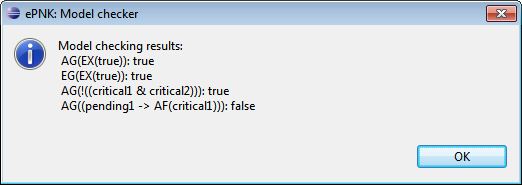
\includegraphics[scale=.40]{ModelCheckingResult.jpg}}
  \caption{Model checking dialog: Result}
  \label{fig:user:modelchecker-result}
\end{figure}


\subsection{Applications view}
\label{subsec:user:applications-view}
\index{ePNK!Application|(DEF}
\index{ePNK!Applications view|(DEF}

As mentioned above, ePNK applications are a bit more involved, since the
user can interact with them, and applications can show some visual feedback
to the user and interact with the user with visual feedback on top
of the Petri net shown in the graphical ePNK editor. One example of such
an application is an interactive simulator for high-level nets, which
is discussed in Sect.~\ref{subsec:user:hlpng-simulator}.

In order to explain the \emph{applications view}%
of the ePNK that is used for controlling the running applications and for
choosing which application the user wants to interact with, we discuss a simple
application: a simple \emph{simulator} for Place/Transition-nets.%
  \index{Simulator P/T-nets@Simulator (P/T-nets)|DEF}

Figure~\ref{fig:user:pt-sim1} shows the ePNK with a P/T-net, two of the net's
pages are open in the graphical editor. At the bottom, the \emph{applications
view} of the ePNK is shown. Note that, initially, the application view is not
open in Eclipse. You can open it in the following way: Choose
``Window''$\rightarrow$``Show View''$\rightarrow$``Other...''; then, in the opened
``Show View'' dialog select ``ePNK: Applications'' from the ``ePNK'' category.%

\begin{figure}[hbt!!]
  \centerline{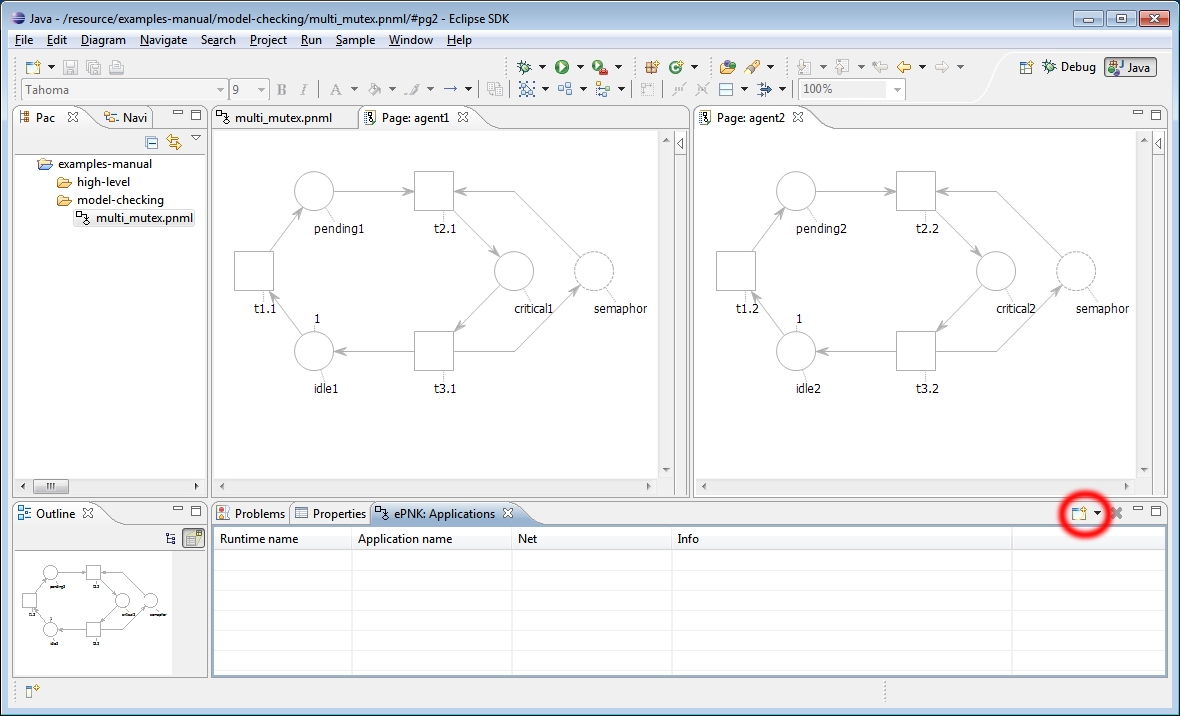
\includegraphics[scale=.30]{pt-sim1.jpg}}
  \caption{Application view a P/T-net in graphical editor}
  \label{fig:user:pt-sim1}
\end{figure}

In Fig.~\ref{fig:user:pt-sim1}, no applications are running yet. When an
editor of a net is selected, you can start an application by selecting
an application from the drop down menu, which is marked by a red circle 
in Fig.~\ref{fig:user:pt-sim1}. This menu will show all registered applications
for the selected Petri net type as well as the option to load an application
that was saved earlier, which we discuss later.

Once you have started the P/T-net simulator, the started application shows
up in the application view, and the net in the graphical editor is decorated
with some additional information. In the case of the simulator, it shows
the current marking as a blue textual label at the top-right of the respective
place; and the enabled transitions are highlighted with a blue overlay.
When the user clicks on these overlays, the respective transition fires.
Fig.~\ref{fig:user:pt-sim2} shows the simulator after the user fired
transitions {\sf t1.2} and {\sf t2.2}. Note that you might not see all graphical
feedback, since some pages are not open in the graphical editor or the graphical
editor is not on the top. You need to open the pages on which you want to see
the feedback yourself.
%
\begin{figure}[hbt!!]
  \centerline{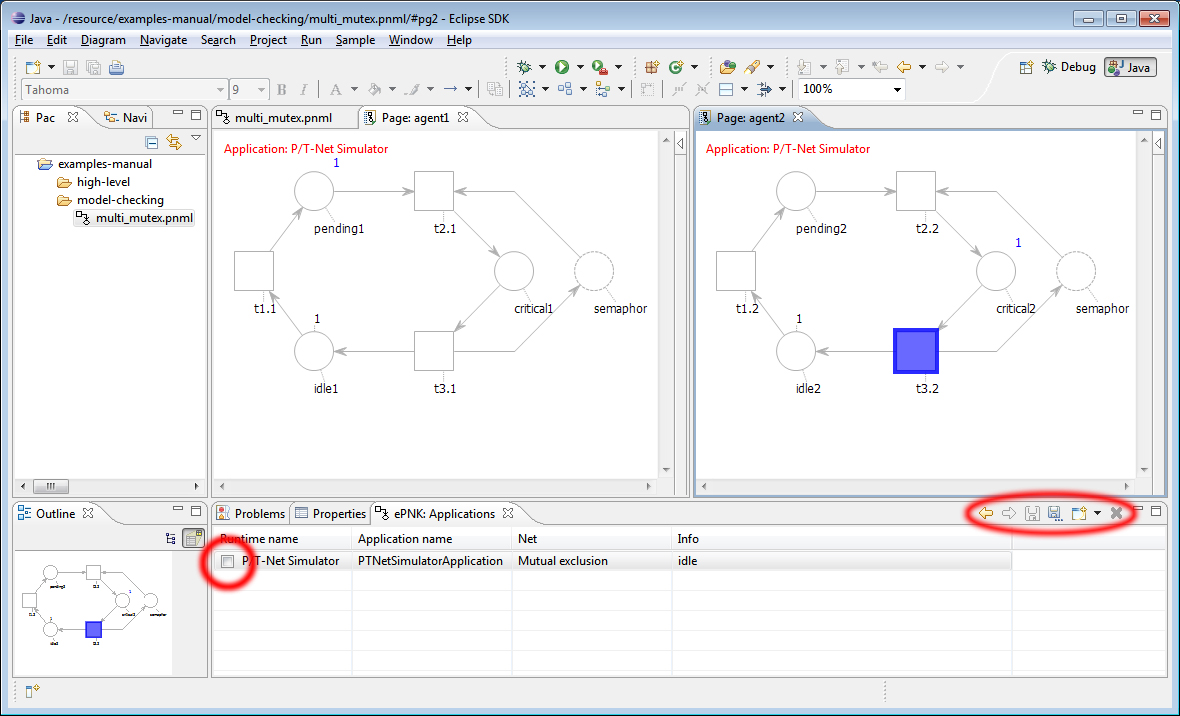
\includegraphics[scale=.30]{pt-sim2.jpg}}
  \caption{Simulator application on P/T-net running}
  \label{fig:user:pt-sim2}
\end{figure}
%
In addition, the application view
shows some more tools in its tool bar (marked in Fig.~\ref{fig:user:pt-sim2})
by a red ellipse. The back and forward buttons allow the user to navigate
to the previous or next markings, and the save buttons allow to save the
state of the simulator. The user can also start further applications by
the respective drop down menu. And the user can shut down an application
by selecting one or more applications by checking the boxes to the left of
an application, and then clicking on the delete tool. Which tools are
shown in the toolbar of the application view depends on the specific
application; but the ones shown in Fig.~\ref{fig:user:pt-sim2} are there
by default and therefore, most applications will have them.

Note that an application is always started from and associated with a net
that is open in an editor. If the editor is closed, all applications on
the respective net are shut down. But, as mentioned above, you can save
the state of an application, so that it can be restarted in that state later.
Fig.~\ref{fig:user:pt-sim3} shows the Eclipse workspace after saving the
state of a simulator by pressing the ``Save as'' button for the simulator
application. In that case the user will be prompted for a folder and file name.
The default is the same name as the net with file extension ``.apnml'' for
annotated PNML. After the first save, the state of the application can be
saved again, by simply pressing the ``Save'' button. 
%
\begin{figure}[hbt!!]
  \centerline{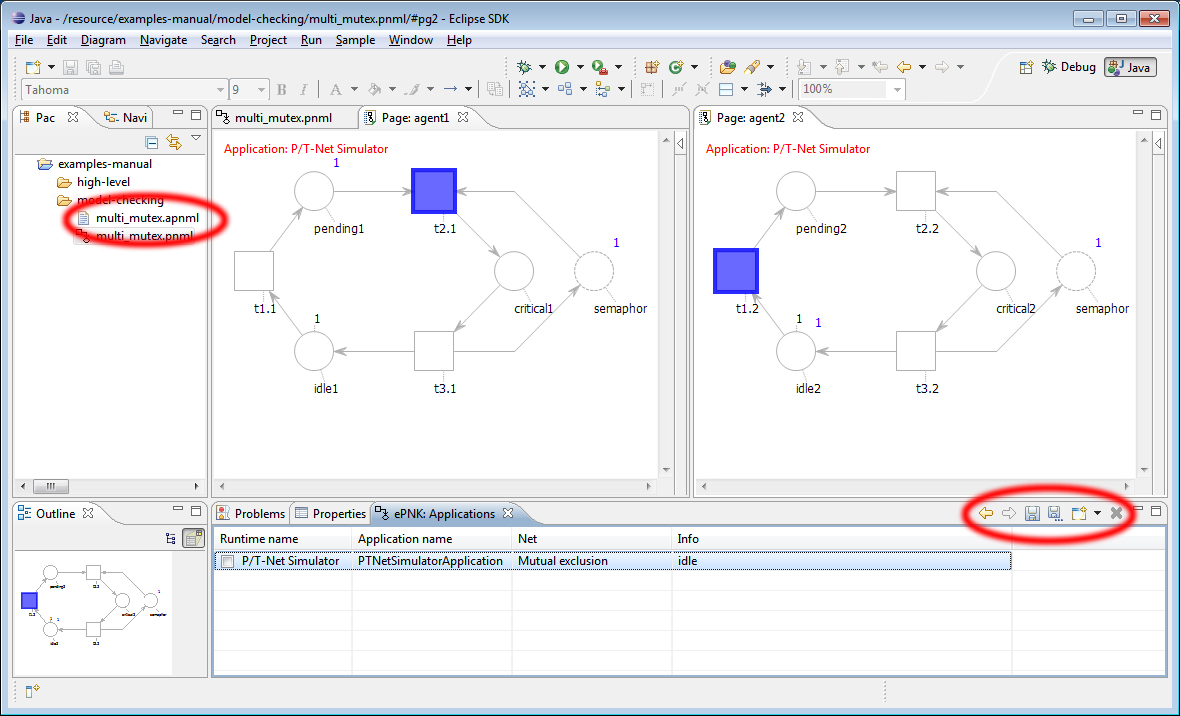
\includegraphics[scale=.30]{pt-sim3.jpg}}
  \caption{Simulator application with a saved state}
  \label{fig:user:pt-sim3}
\end{figure}
%
Later the application can be started by the drop down menu selecting
``Load application'' and then selecting the file to which the state was saved
before.

Note that there is always at most one application \emph{active}%
  \index{active application|DEF}
in the ePNK, and only the decorations of this active application are shown in
the graphical editor. But, there can be many applications running at the same time.
All running applications are shown in the applications view, and by selecting
an application there, it becomes active. You can also deselect an active
application by clicking on it with the CTRL-button pressed at the same time.%
  \index{ePNK!Applications view|)}%
  \index{ePNK!Application|)}

\subsection{A simulator for high-level nets}
\label{subsec:user:hlpng-simulator}
\index{Simulator|(DEF}

In this section, we discuss the simulator for high-level Petri nets, which is
deployed together with the ePNK. It was developed by Mindaugas Laganeckas as
part of his master's project \cite{Lag12}. The simulator is able to
simulate high-level Petri nets as well as so-called \emph{high-level net schemas}%
  \index{High-level net schema}
\cite{KiRe96,KRVW97,Rei98,HKea09,ISO-IEC:15909-2-2011}, which can
be instantiated with some communication network in order to simulate
a network algorithm on a specific network \cite{RKea98}.

Note that all examples that are discussed in this section can be obtained
from the ePNK home page together with release 1.0.0 of the ePNK:
\url{http://www2.imm.dtu.dk/~ekki/projects/ePNK/release-1.0.0.html}.

\subsubsection{The basic simulator for high-level nets}
\label{subsubsec:user:sim:basic}

We start with explaining the simulator for normal high-level nets in this
subsection and explain the simulator for net schemas later in Sect.~\ref
{subsubsec:user:sim:networks}.

Figure~\ref{fig:user:hl-simulator-1} shows the simulator application running
on a simple high-level net. The high-level net models a simple algorithm that
computes the prime numbers according to the principle of the ``Sieve of
Eratosthenes'':%
  \index{Sieve of Eratosthenes}
It starts with a multiset of all the numbers from $2$ up to some upper limit
($11$ in our example) on place {\sf numbers}. Then, the transition {\sf t}
removes a number (the value of {\sf x*y}) from this place, if this number is a
multiple of some other number (the value assigned to {\sf x}) on that place.
When no number on the place is a multiple of another number on that place, 
the transition cannot fire anymore -- and the algorithm terminates. The
numbers that are left on place {\sf numbers} are prime numbers.
%
\begin{figure}[hbt!!]
  \centerline{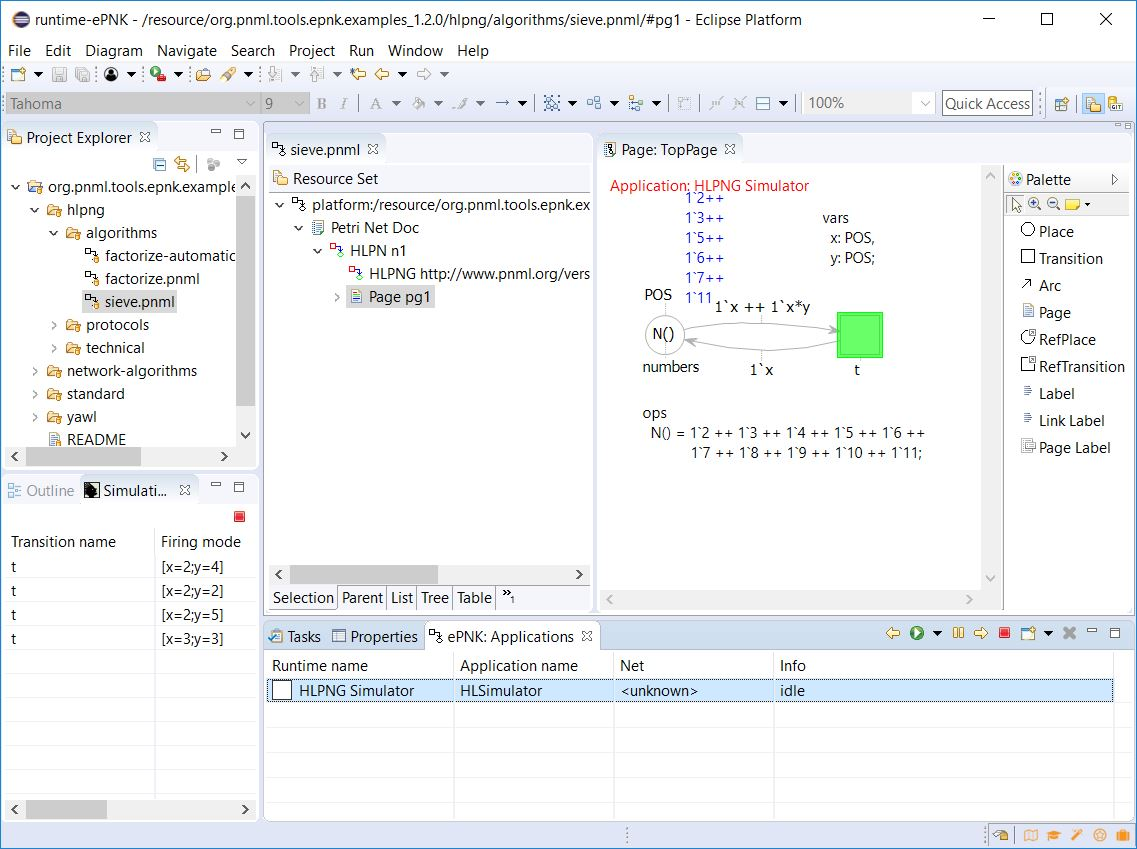
\includegraphics[scale=.33]{HL-SimulatorPrimes}}
  \caption{ePNK with a simulation application running on a HLPNG}
  \label{fig:user:hl-simulator-1}
\end{figure}
%
In Fig.~\ref{fig:user:hl-simulator-1} there is only one last non-prime
number left: $6$. The current marking of the place is shown as a blue
label at the top-right corner of the place (a long stack of tokens
represented as a multiset term in the concrete syntax for HLPNGs of the
ePNK).

Assuming that you have obtained and installed the examples from the ePNK home
page, we will now explain how to start the simulator and how to open the
additional simulator view, which shows the firing sequence up to the latest
point in the simulation. Then we will explain how to interact with the simulator.

If you did not do that yet, you need to open the \emph{ePNK applications view}%
  \index{ePNK!Applications view}
as described\footnote
  {In short:
   Choose ``Window''$\rightarrow$``Show View''$\rightarrow$``Other...'';
   then, select ``ePNK: Applications'' from the ``ePNK'' category.}
in Sect.~\ref{subsec:user:applications-view}. The \emph{Simulation view}%
  \index{Simulation view|DEF}
can be opened in a similar way: Choose
``Window''$\rightarrow$``Show View''$\rightarrow$``Other...''; then, in
the ``Show View'' dialog, select ``Simulation View'' from the ``HLPNG
Simulator Category''. By clicking on the tab at the top of the views,
you can arrange them in a way similar to Fig.~\ref{fig:user:hl-simulator-1}
-- it is convenient to see the applications view and the simulation view
at the same time.

The simulator can be started on a high-level net by right-clicking on the
HLPNG element in the ePNK tree editor and then selecting 
``ePNK''$\rightarrow$ ``Start Simulator App''.

Once the simulator application is started and selected in the applications view,
the simulation view shows the firing sequence of all transitions (along with the firing mode)
from the initial marking up to the last step of the current simulation.
If no simulation application is selected, the simulation view shows the
firing sequence of the last active simulation.  You can click on the different
entries and navigate up and down with the resp.\ buttons of the keyboard; then
the net will show the marking before the selected transition fired. The
current marking for each place is shown as a blue label at the
top right of every place -- if there is no label, the place's marking is
currently empty.

When a simulator application is selected in the applications view, you will
find several action buttons on the top right of the applications view, which
can be used to control the simulator (as shown in
Fig.~\ref{fig:user:hl-simulator-1}). The \emph{back}%
  \index{Simulator!Back button|DEF}
(left arrow) and \emph{forward}%
  \index{Simulator!Forward button|DEF}
(right arrow) buttons allow you to
navigate back and forth in the firing sequence (which had been simulated
already). The \emph{play button} (white triangle in green circle), starts the
\index{Simulator!Play button|DEF}
automatic and random firing of some transitions -- as long as there are
enabled transitions. The \emph{simulation speed}%
  \index{Simulator!Simulation speed|DEF}
can be selected by a drop
down menu on the small triangle right of the play button. It can actually
be changed while the automatic simulation is running. The automatic
simulation can be stopped -- actually ``paused'' -- by the pressing the
\emph{pause button}.%
  \index{Simulator!Pause button|DEF}
The automatic simulation can be started any time by pressing the play button
again. By pressing the \emph{stop button},%
  \index{Simulator!Stop button|DEF}
(red box), the simulator is reset to the initial marking as defined by
the net. The cross to the right will delete the simulator completely
(actually this is the general control for all applications).

The automatic simulation will randomly choose any of the currently activated
transitions, and randomly choose a firing mode. If the simulation is paused,
however, the activated transitions are high-lighted by a green overlay. You
can click on these green transitions\footnote
  {You will also be able to click on a transition which is high-lighted in grey
  or blue, as will be discussed later.}%
; then, a menu will pop up, which shows all the possible firing modes for
that transition from which you can select. Then, the transition will be
fired in the selected mode. Clicking somewhere else or pressing the ESC
button, will cancel the selection though.

Note that if you go back to some earlier state of the simulation by
selecting a transition in the simulator view or by the back button in
the simulator application, the marking at that point in the firing sequence
will be shown. You will see that one transition is high-lighted by a
blue (and darker) overlay. This is the transition to fire next in the
firing sequence as shown in the simulation view. There might also be
some other transitions high-lighted by a green overlay, which would
have been alternative choices at that point. Note that also a blue
transition might ``hide'' alternative choices that are not graphically
high-lighted, since it might be able to fire it in different firing modes.

If you are in such an intermediate state of a firing sequence, you can
still interact with the transitions by clicking on them as discussed
above and by selecting a firing mode, which will fire this alternative
transition in that marking. Note that in this case, all the later firing steps
of the earlier firing sequence are deleted.
From the current point on, a new branch of simulation will be followed.
This way, you will be able to explore different branches of the reachability
graph of the Petri net.

Note that, in some cases, the simulator is not able to compute the firing modes
fully automatically, and is not able to decide whether a transition is enabled.
In that case, the respective transition is high-lighted with a grey overlay.
This does not happen in the prime factors example, but it will happen all-over
in the example ``factorize''. Once you click on one of the transitions with a
grey overlay, you will be prompted for possible values for the different
variables. You can enter a semicolon separated list of values for each of the
variables; then the simulator will try to compute possible firing modes based on
these values.  Note that you do not need to provide values for all variables; in
many cases, it is enough to provide the value for one variable from which the
values for the other variables can be derived.  If the simulator can compute
some enabled firing modes, the transition will be high-lighted in green, so that you can
actually select the mode in which this transition should fire. You can still select
``Manual input'' for providing more or other possible values.
If no modes could be found, the transition will remain high-lighted in grey;
only if you provide values for which the transition can fire (or enough
information for the simulator to figure that out), the transition will actually
become enabled.

\subsubsection{Supported operations}
\label{subsubsec:user:sim:supported}

Note that the simulator is still in an experimental phase. In particular, some
of the more specific operations of ISO/IEC~15909-2 are not supported yet. This,
in particular, applies to the sorts and operators for symmetric nets
which currently are not supported by the simulator.

The following sorts of ISO/IEC~15909-2 are supported in the current
version (0.1.2) of the simulator: {\sf DOT}, {\sf BOOL}, {\sf NAT}, {\sf POS},
{\sf INT}, and {\sf STRING} as well as the generic sorts product, multiset
and lists over existing sorts.

The following operators are supported:
{\sf ==} and {\sf !=} on all sorts;
{\sf or} and {\sf and} on {\sf BOOL};
{\sf +}, {\sf -},  {\sf *},  {\sf /}, {\sf \%}, $<$,  and $>$ on
{\sf NAT}, {\sf POS} and {\sf INT};
{\sf concatstring} for Strings;
{\sf '}, {\sf ++}, {\sf -\,-}, {\sf all}, and {\sf empty} on multisets;
the tuple operator for products; 
{\sf emptylist}, {\sf makelist}, {\sf memberat}, {\sf sublist}, {\sf length},
{\sf appendtolist}, and {\sf concatlists} for lists.

The sorts and operators introduced for symmetric nets are not
supported by the simulator at all.
 
\subsubsection{The simulator for network algorithms}
\label{subsubsec:user:sim:networks}

In this section, we discuss the simulator for network algorithms. Before
discussing the simulator itself, we discuss the concept of network
algorithms and the way they are modelled as algebraic nets schemas
or -- in the terminology of ISO/IEC~15909 -- high-level Petri net schema
(HLPNGS).%
  \index{HLPNGS|DEF}
To this end, we use an example which -- except for syntactic sugar --
is almost identical to the first publications that used algebraic
net schemas for modelling and verifying network algorithms%
  \index{Network algorithm}
\cite{KiRe96, WWea97, Rei98}: a simple algorithm that, for a given network
of computing agents with some distinguished root agents, computes the
minimal distance of each agent from a root agent. The Petri net modelling
the algorithm is shown in Fig.~\ref{fig:user:sim:mindistance-exmpl}.%
  \index{Minimal distance algorithm}
%
\begin{figure}[hbt!!]
  \centerline{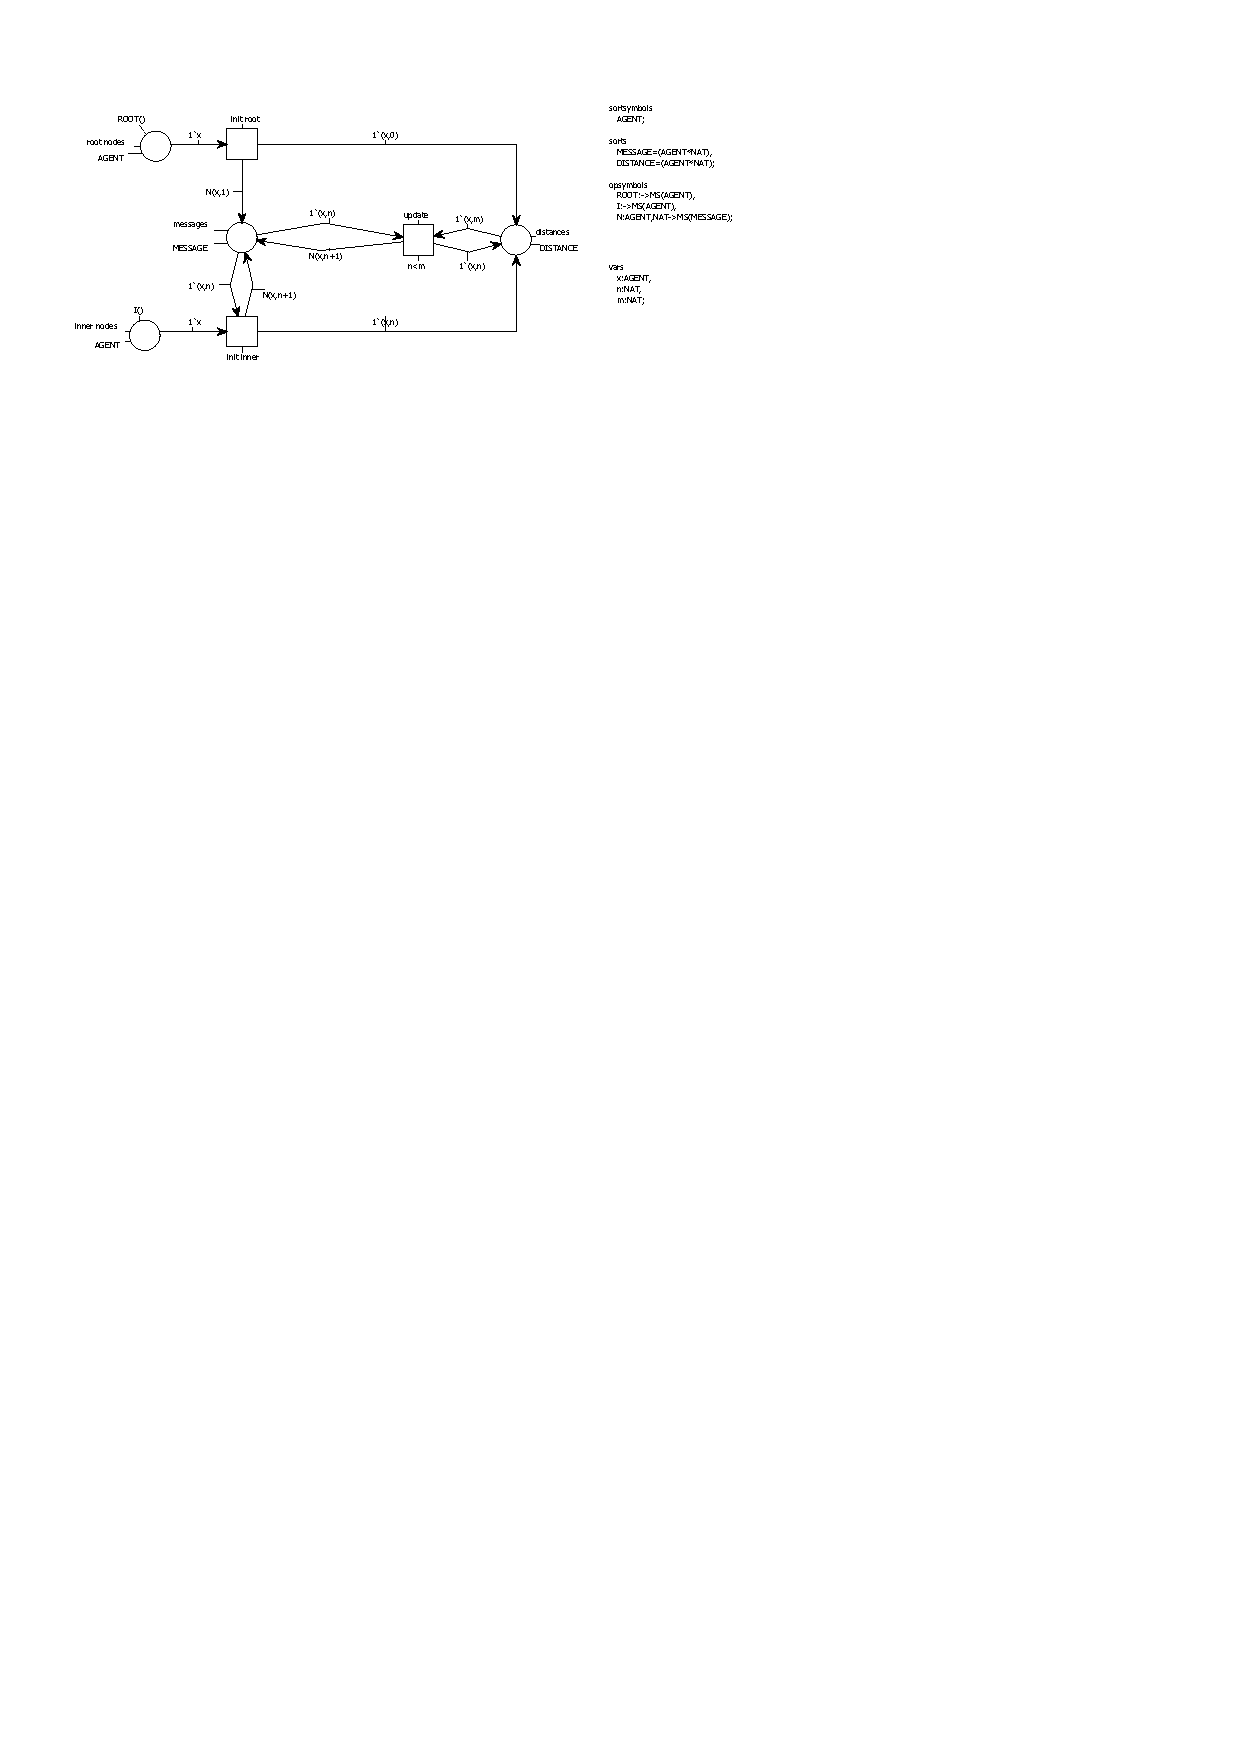
\includegraphics[scale=1.0]{MinDistance}}
  \caption{Network algorithm computing the minimal distance to a root}
  \label{fig:user:sim:mindistance-exmpl}
\end{figure}
%
In the example projects deployed for the ePNK 1.0.0, you will find it
in subfolder min-distance of folder network-algorithms.

One of the main features of a Petri net schema is that, the Petri net
model itself is completely independent from the actual network of
agents on which the algorithm is working. In the model from
Fig.~\ref{fig:user:sim:mindistance-exmpl}, the set of agents of
the network is represented by the sort {\sf AGENT}, but it is
just a symbol -- which still needs some interpretation. The
multiset constant {\sf ROOT} represents the set of root nodes,
and the constant {\sf I} represents the set of non-root nodes
(or inner nodes).

Moreover, there is an operation {\sf N}, which takes an {\sf AGENT}
and a natural number as a parameter. This function represents
sending a message from one agent to all its neighbours in the
network -- where the message itself is a natural number. A
{\sf MESSAGE} to an agent is represented by a pair, where the
first component is the receiver {\sf AGENT} and the second component
is the actual content of a message. If there is a distance computed
for some agent already, this is also represented as a pair of
an {\sf AGENT} and a number {\sf NAT} -- for making the difference
clear, we call this pair {\sf DISTANCE}.

Initially, the place {\sf root nodes} contains all the root nodes
of the network; the place {\sf inner nodes} contains all the inner
nodes. The transition {\sf init root} models the initial step of a
root node $x$: it sets its own distance to $0$, which is represented
as a pair $(x,0)$, and adds a message to all its neighbours that
they might have distance $1$ from a root node -- all these messages
are represented by $N(x,1)$. Transition {\sf init inner} models
the initial step of an inner node: when an inner node $x$
initially receives some message with some distance $n$, it stores
this distance as a potential shortest distance, and sends a
message to all its neighbours with distance $n+1$, which is
represented by $N(x,n+1)$. An inner node $x$ can later receive
other messages with another distance $n$; if the other
distance $n$ is less than its current distance $m$, the agent
takes distance $n$ as its new distance, and sends a message with
distance $n+1$ to all its neighbours. This is modelled by transition
{\sf update}.

As said before, the Petri net model from
Fig.~\ref{fig:user:sim:mindistance-exmpl} models an the minimal
distance algorithm for any network. If we want to simulate the
algorithm, we need to know on which network it should run. To this end,
a very simple network editor is deployed together with the high-level
simulator of the ePNK. Figure~\ref{fig:user:sim:network} shows the
network editor with a simple example network. In this case, it
is a network with directed arcs.
%
\begin{figure}[hbt!!]
  \centerline{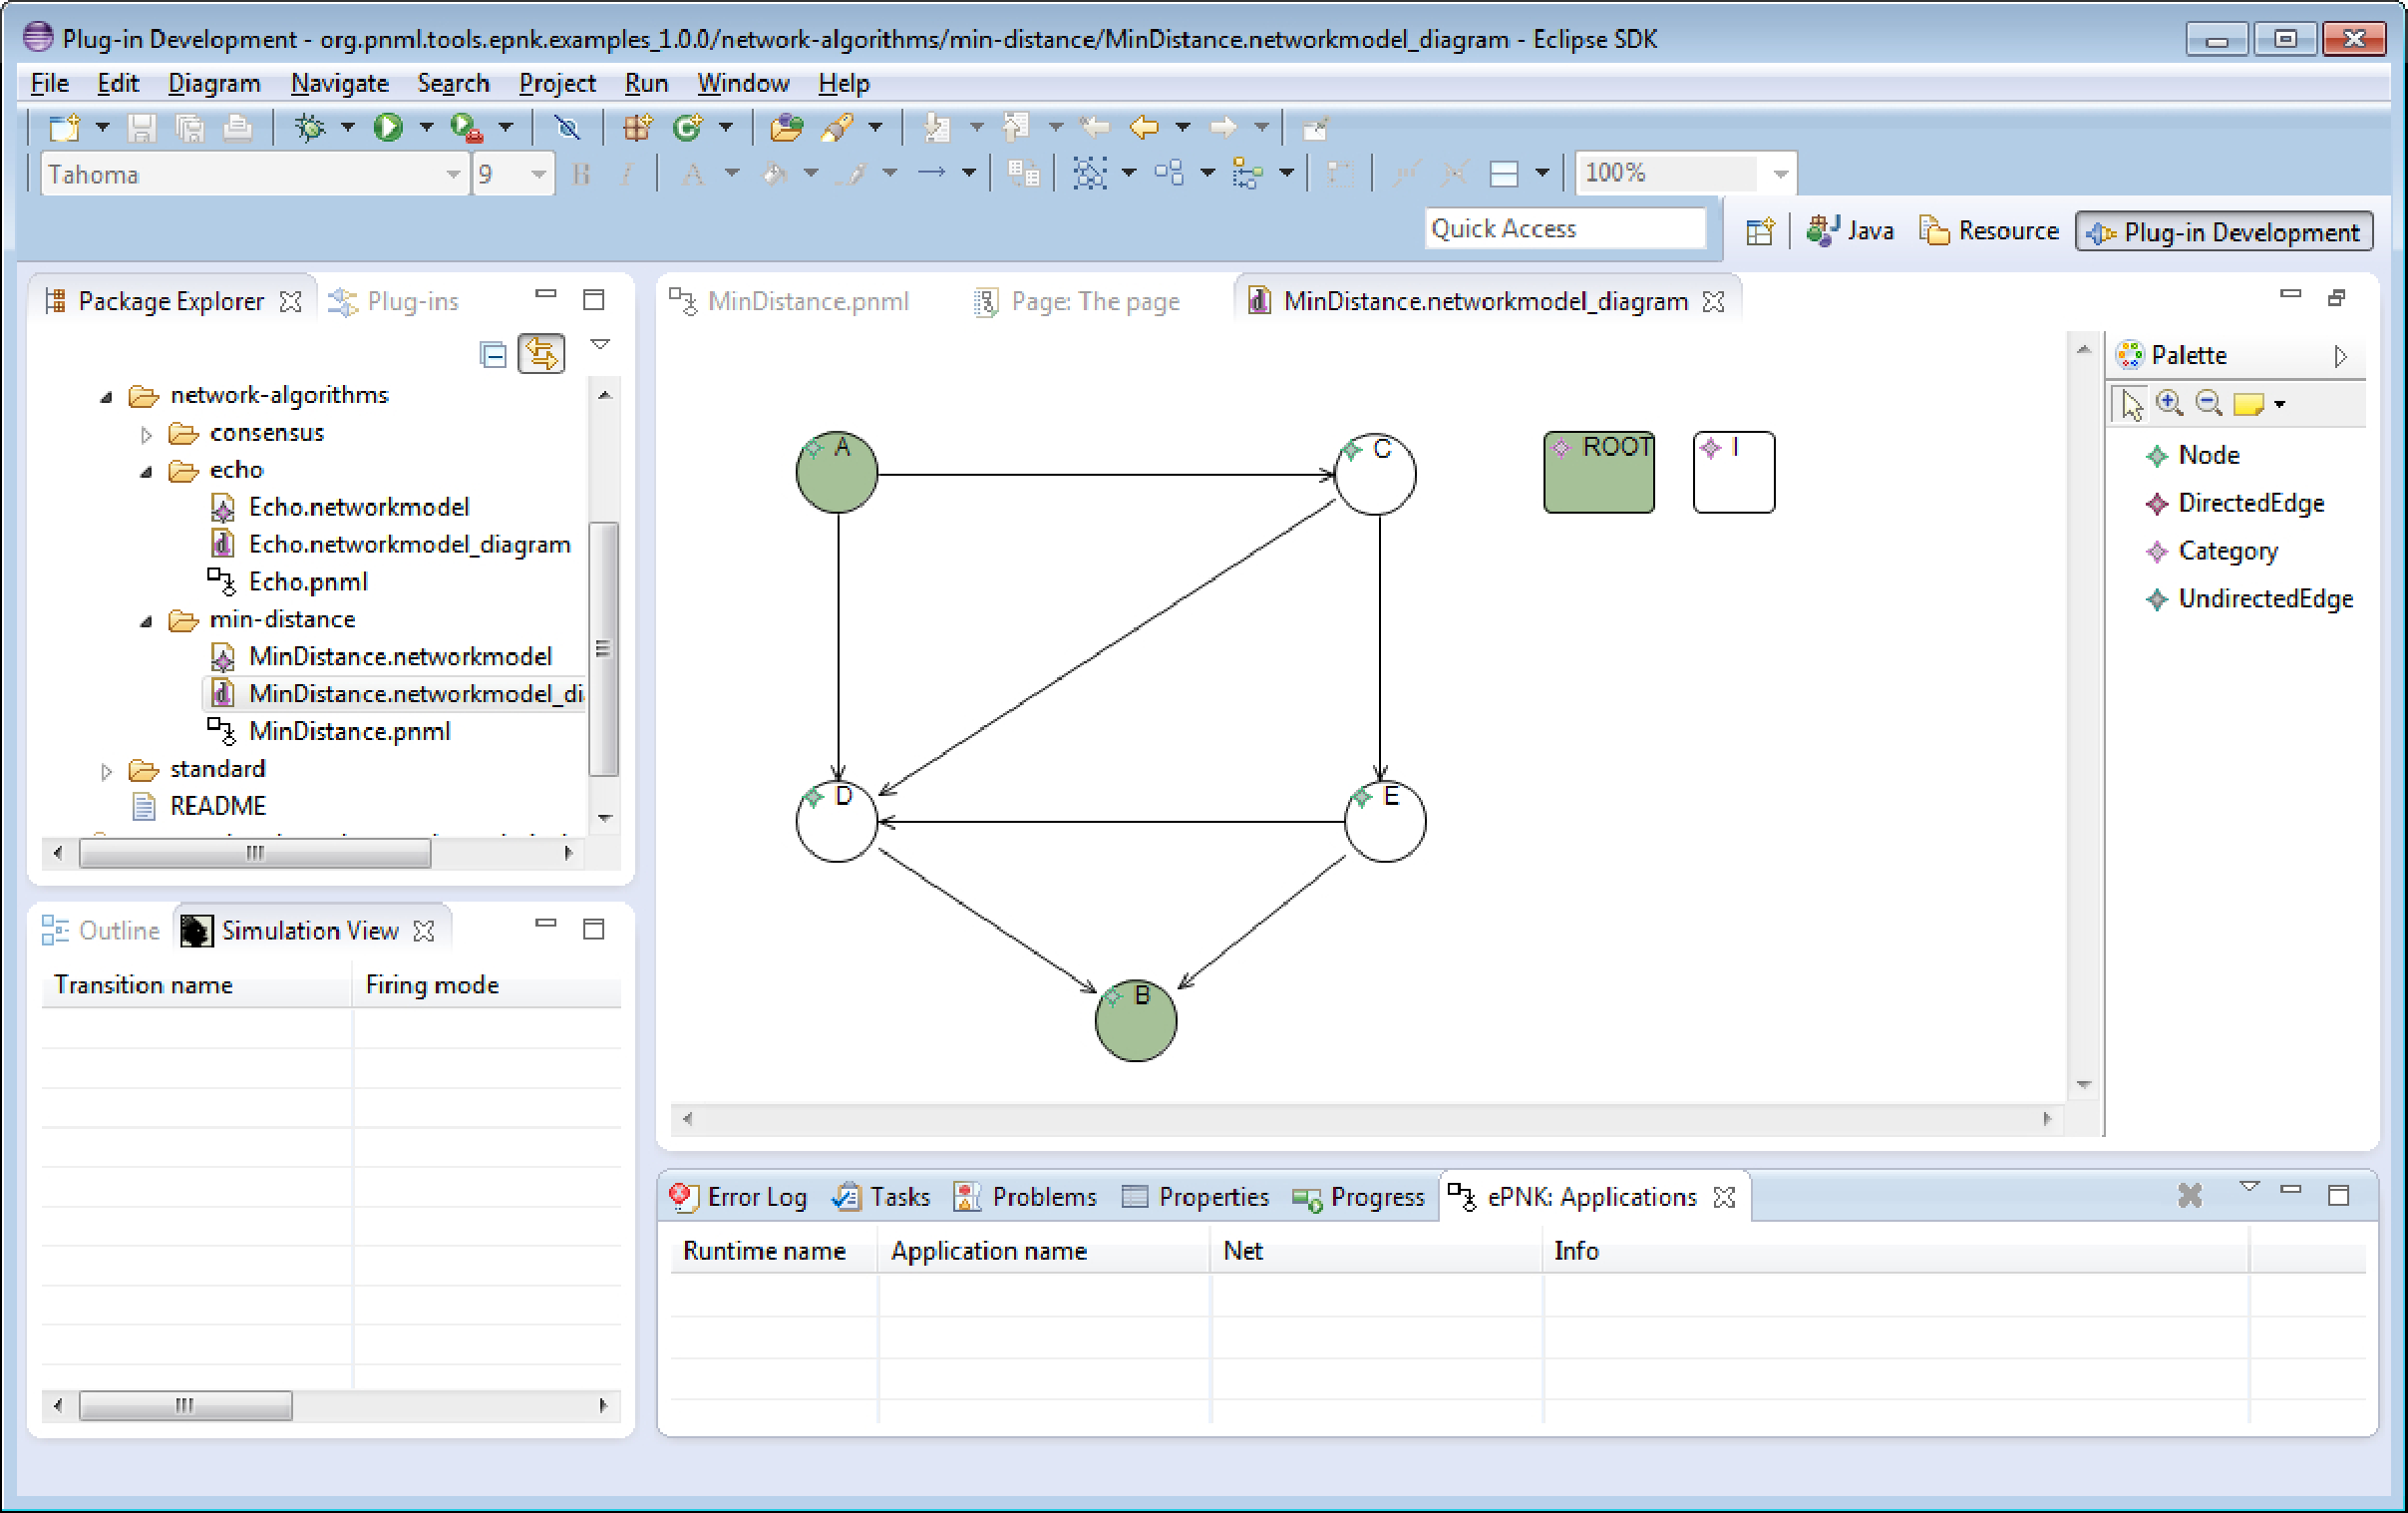
\includegraphics[scale=0.3]{Network}}
  \caption{A network on which the algorithm could work}
  \label{fig:user:sim:network}
\end{figure}
%
The network simulator can be started by right-clicking on the HLPN element in
the ePNK tree editor and then selecting ``ePNK''$\rightarrow$``Start Network
Simulator App''; if there is a network file with the same name as the Petri
net model in the same folder, the network simulator chooses this network for
the simulation. If there is no such file, the user will be prompted for
a file with a network model. Once the network model is selected, the
interpretations of the sort {\sf AGENT}, the constant symbols {\sf ROOT}
and {\sf I}, as well as the function {\sf N} (sending a message to all
the neighbours of the agent) are defined by this network. For example, for
the network of Fig.~\ref{fig:user:sim:network}, the set associated with
the sort {\sf AGENT} is $\{ A, B, C, D, E \}$; the constant {\sf ROOT}
denotes the multiset $[A, B]$, the constant {\sf I} denotes the multiset
$[ C, D, E]$; for $x = A$ and $n = 5$, the term {\sf N(x,n)} will evaluate to
the multiset $[ (C,5), (D,5) ]$ -- representing the message $5$ to each neighbor
of agent $A$. And these will be the interpretations the simulator will be using
for simulating the net.

Figure~\ref{fig:user:sim:mindistance-sim} shows the network simulator running
on the minimal distance algorithm from
Fig.~\ref{fig:user:sim:mindistance-exmpl} on the network from
Fig.~\ref{fig:user:sim:network}.
%
\begin{figure}[hbt!!]
  \centerline{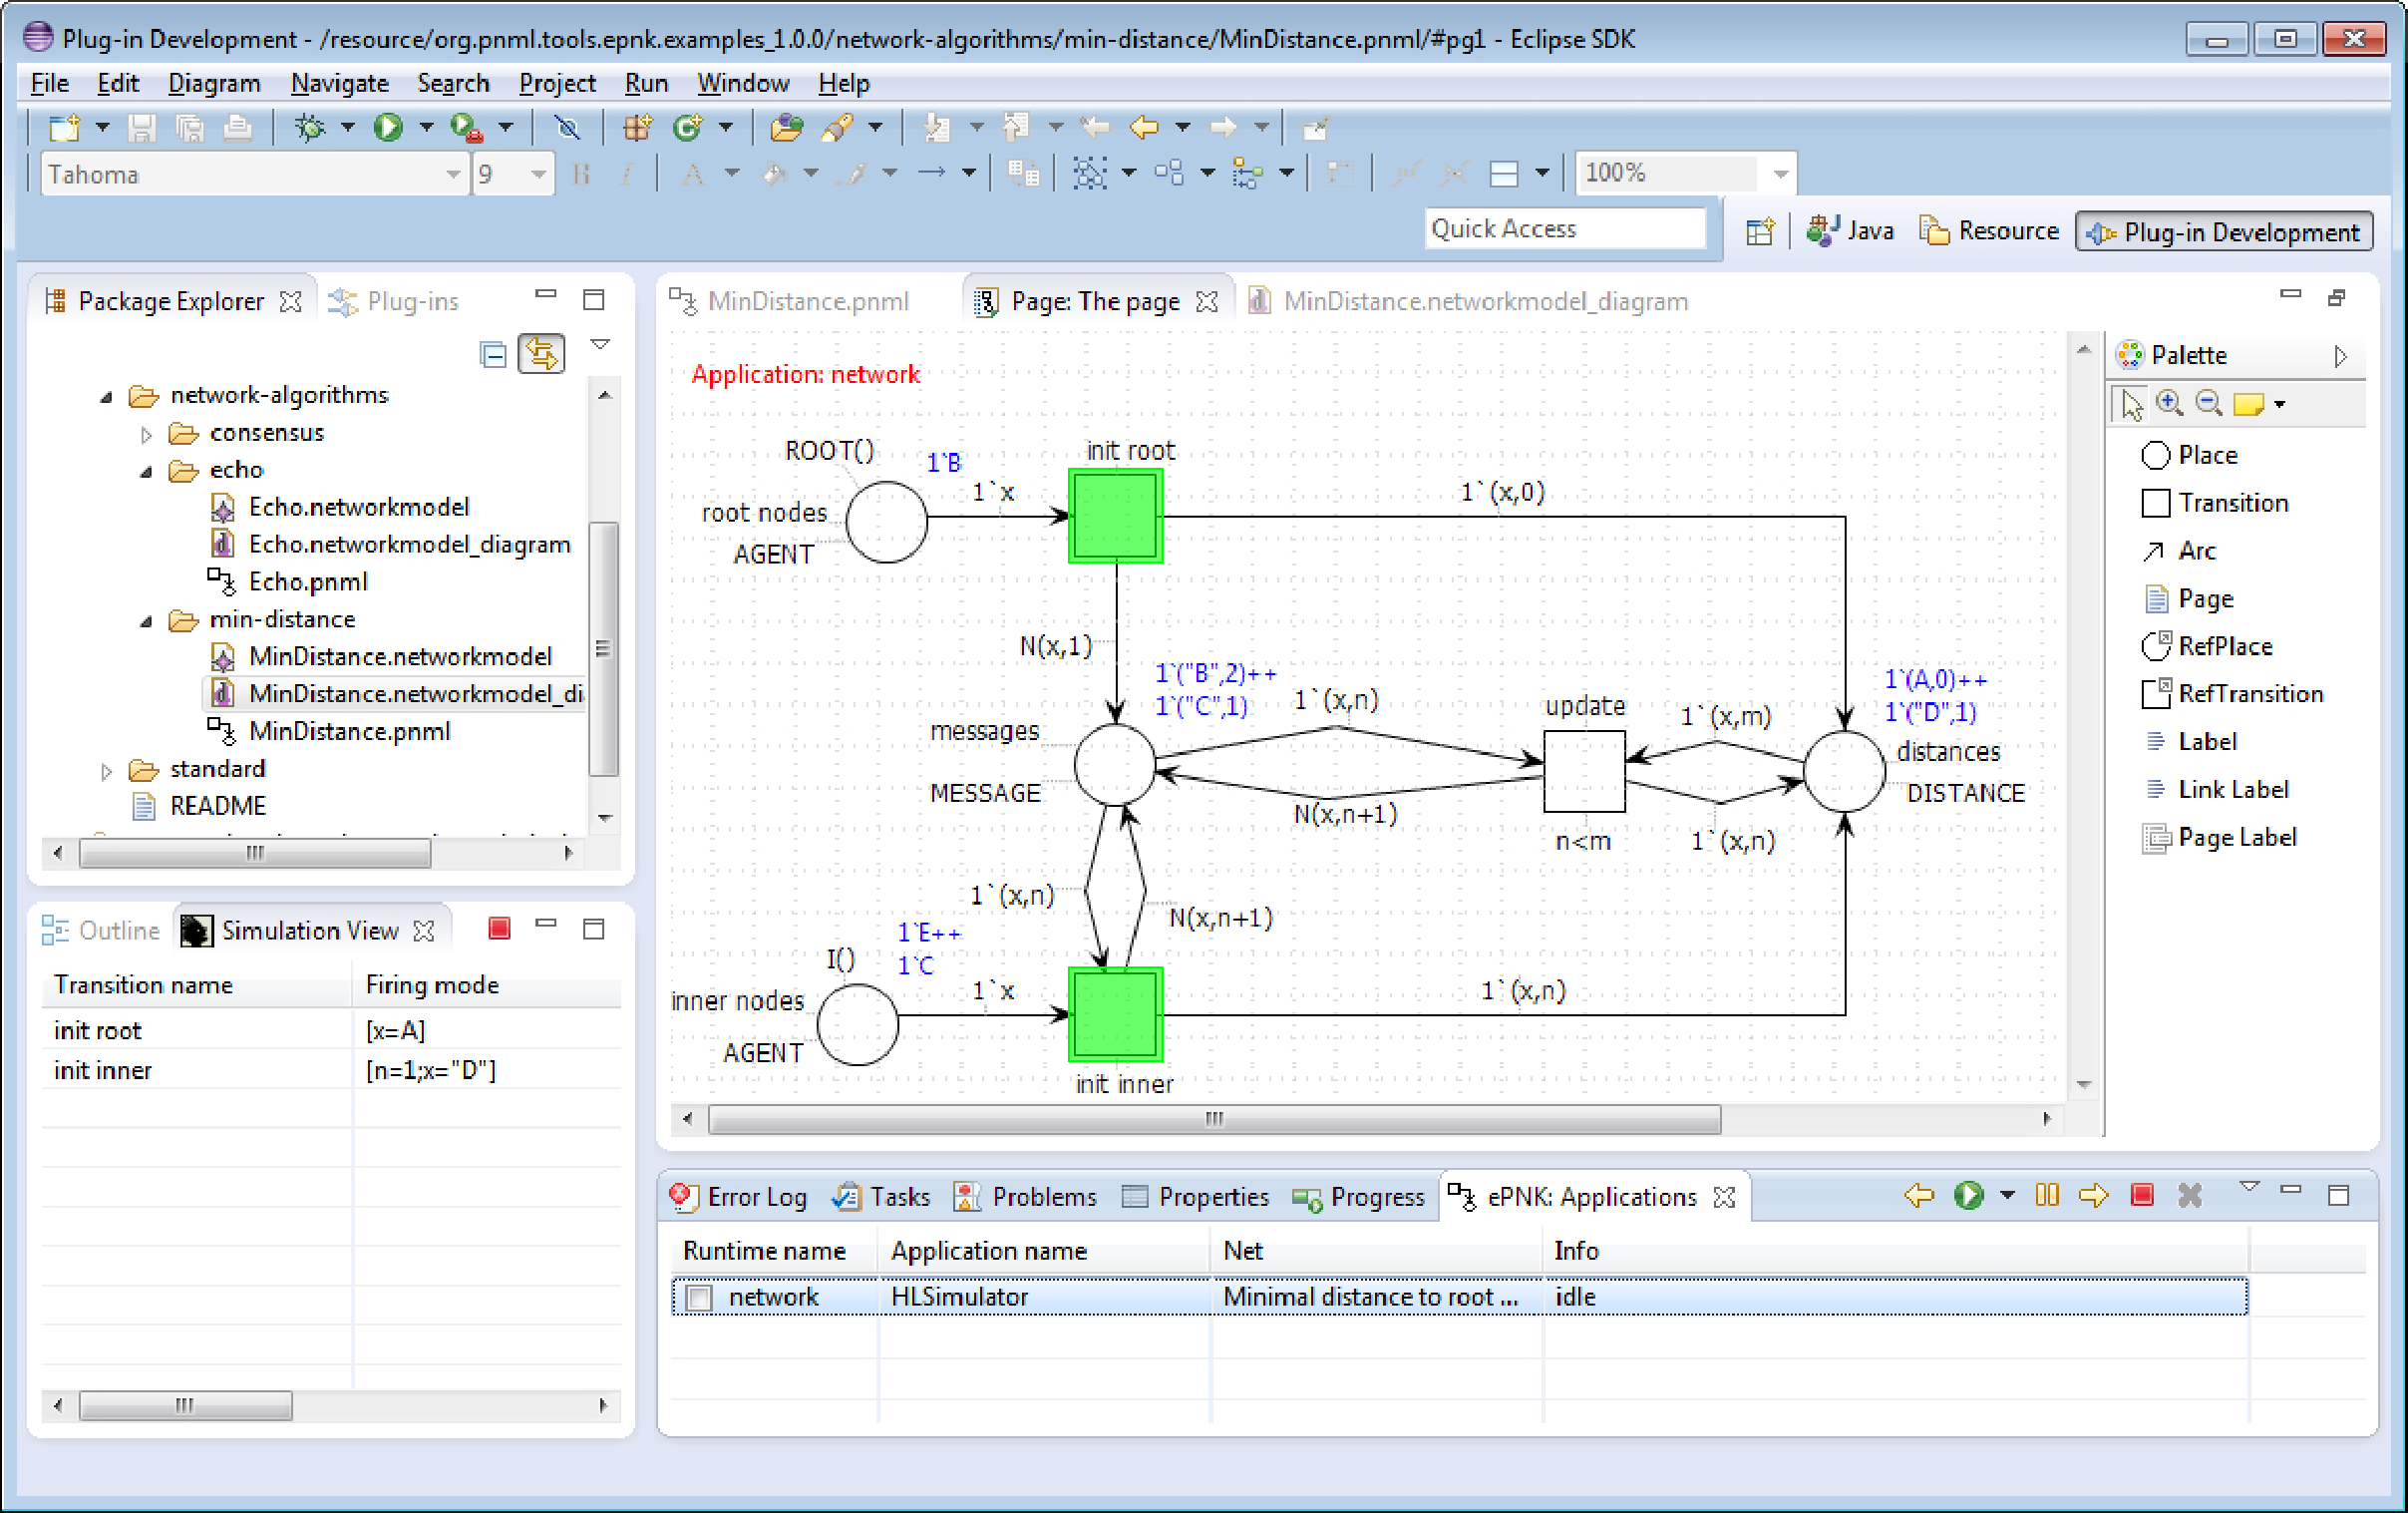
\includegraphics[scale=0.3]{MinDistanceSimulator}}
  \caption{Network simulator running on the minimal distance algorithm}
  \label{fig:user:sim:mindistance-sim}
\end{figure}
% 
The interaction with the simulator and the way to control the simulation is
exactly the same as described for the basic simulator in
Sect.~\ref{subsubsec:user:sim:basic}, once the network simulator is
properly initialized with a network.

The editor for the \emph{network}%
  \index{Network model}%
  \index{Network editor|DEF}
is a simple \emph{editor} generated by GMF
and follows the GMF philosophy. A new network can be created by
``File''$\rightarrow$ ``New''  $\rightarrow$ ``Other...'' and then
selecting ``Network Diagram'' from category ``Examples''. In this
diagram, you can add nodes, directed and undirected edges between the
nodes, as well as categories for nodes. When a node is selected,
each node can be associated with any number of categories by
a menu that pops up when clicking in the category property in
the properties view. In Fig.~\ref{fig:user:sim:network}, the
association with categories is also shown by the same colour for
the category and the resp.\ nodes; but the colour itself does not have
any meaning in the diagrams.

For a given network, the sort {\sf AGENT} is associated with
the set of nodes; for every category, the respective constant
symbol is associated with the multiset of nodes that are in
that category (in our example these are the root nodes and
the inner nodes). For the operation symbol {\sf N}, 
$N(x,m)$ denotes a multiset of pairs, where for each outgoing
arc from $x$ to $y$ there is a pair $(y,m)$ in the multiset.
$S(x)$ is a multiset of pairs over agents, where there
is a pair $(y,x)$ in the multiset if there is an undirected
arc from $x$ to $y$; these represent all messages that are
sent from agent $x$ to all its neighbours. Likewise $R(x)$ contains
all the messages received from all its neighbours. 

A Petri net modelling the echo algorithm,%
  \index{Echo algorithm}
which is another example deployed together with the ePNK, makes use of the send
and receive operations {\sf S} and {\sf R}. But, we do not explain the echo
algorithm here -- see \cite{WWea97, KRVW97} for details\footnote
  {The operation {\sf S} is denoted with $M$ and the
   operation {\sf R} is denoted with $\overline{M}$ in \cite{KRVW97} -- and
   the other way round in \cite{WWea97}.}%
.%
  \index{Simulator|)}

\section{Limitations and pitfalls}  

The current version of the ePNK (1.0.0) still has some minor limitations,
which are discussed in this section in order to avoid some unpleasant
surprises. If you identify other issues or problems, please, let us know. 
  
\subsection{Saving files: Tree editor}
Technically, the tree editor and the graphical editor for pages are
different editors. The graphical editors can be initiated via
the tree editor only (via the pop-up menu ``Start GMF Editor on Page'' or
a double click on a page in the tree editor or the graphical editor).
The tree editor, however, serves as the main editor; saving a PNML document
is possible only from the tree editor -- and only the tree editor
shows a valid ``dirty-flag'' when the file contains unsaved changes
(see Sect.~\ref{subsec:save-documents})

\subsection{Reset an attribute}
\label{subsec:user:reset-attribute}
In case some attribute is set to some value and you would like to remove
that value (meaning that actually, the attribute is removed completely),
it is no good to enter an empty string as a value for that property. And
if it is an attribute with finitely many possible values, the drop down
menu does not give you an option to not select any value. To restore
the default situation of unsetting the attribute, you can right-click
into the property column of that attribute in the properties view and then
select ``Restore default value'' (see Sect.~\ref{subsec:attributes}).


\subsection{Graphical features}
\label{subsec:supported-graphical-features}

The graphical editor of the ePNK supports many graphical features, such as
positions and size of nodes, intermediate positions for arcs, fonts, size and
colours for labels, colours and line-width for nodes and arcs. Up to now, not
all of these graphical features are transferred back to the actual
PNML document (some of this information it is not even supported by PNML).
Some graphical information is stored only as (ePNK) tool specific information.

The graphical information that is used and made available in PNML
so that it can be used by other tools that support PNML is the following:
\begin{itemize}
  \item Position and size of nodes.
  \item Line colour and background colour for nodes.
  \item Image information for nodes\footnote
          {Up to version 1.0.0 of the ePNK, the path to an image can be changed
          only in the tree editor. But the image is shown in the graphical editor
          once it is set. From version 1.0.1 and higher, it will be possible to
          set the image URI in the properties view of the node directly}.
  \item Position resp.\ relative position of labels\footnote
          {The size of labels is not supported by PNML}.
  \item Text colour\footnote
          {For the text colour the ePNK is actually abusing the line colour
           attribute of PNML, since PNML does not have a text colour
           attribute.}
        and background colour for labels.
  \item The font and the font-size of labels.
  \item Intermediate points of arcs.
  \item Line colour of arcs.
  \item The shape attribute of arcs (straight or bezier).
\end{itemize}

Note that all the graphical information -- even the one that is not transferred
to PNML features -- is saved by the ePNK as tool specific information. You can
even put notes on the graphical canvas, which will be saved. The graphical
information not covered in the above list, however, will not be available to
other tools, and will be gone, when the tool specific information
(org.pnml.tools.epnk.diagraminfo) for the resp.\ page is deleted.

The ePNK reads all graphical attributes that are supported by PNML;
but, only the ones discussed above are used and shown in the graphical editor.
Moreover, the unused graphically attributes are not checked for
validity; they will be written exactly the same way they were, when
loading the PNML file (see also Sect.~\ref{subsec:graceful-PNML}).

Due to some limitations in the automatically generated GMF editor on which
the graphical editor of the ePNK for pages is based, there is another quirk
of the graphical ePNK editor: When a node is moved, the intermediate points of
the attached arcs are also changing in the diagram; these changes are, however,
not propagated to the PNML model. If you want to make sure that the
intermediate points of an arc of the diagram and the PNML are exactly the same,
the you need to explicitly touch and slightly move an intermediate point of each
attached arc -- only then, the exact positions of the intermediate points
are properly propagated to the PNML model.

Note that some Petri net type definitions might define some graphical appearance
for some of its elements. In that case, this graphical appearance overrides the
graphical attributes of PNML.

\subsection{Petri net types}

As mentioned in Sect.~\ref{subsec:creating-elements}, the type of a Petri net
should never be changed after a net of that type was created --
unless you know exactly what you are doing. Otherwise, it could happen
that the produced PNML is invalid.

For HLPNGs, it is no problem to change its kind any time, since this
kind has an effect on the validation only, but no effect on the
serialisation of the net to a PNML file. Changing the ``kind'', actually,
does not change the Petri net type -- just the sub sets of features that
are supported.

 
\subsection{Wrapping labels}

All labels in ePNK can have line-breaks. In the graphical editor,
line-breaks can be added by pressing the CNTRL and ENTER at the same time.

\subsection{Graceful PNML interpretation}  
\label{subsec:graceful-PNML}

PNML files that are produced by the ePNK and which have been successfully
validated are conformant to PNML as defined in ISO/IEC~15909-2. The
only exception is, when some illegal graphical attributes are read from an
existing PNML file; these attributes will not be touched by the ePNK, and
therefore written again -- even if they are not conformant to ISO/IEC~15909-2.
But, if a PNML file is created by using the ePNK only and if it validates
correctly, the saved file is PNML conformant.

The ePNK, however, is not a PNML validator. It reads PNML and ``PNML-like''
documents and writes them again in a graceful manner. This way, it is possible
to save PNML documents that do not properly validate; and the ePNK is able to
load these files again even though other PNML tools might not be able to
load them. For example, when some elements do not have ids (as required
by PNML), references to these elements cannot be made via their id. In that
case, the ePNK uses XPath references to these elements, which is not conformant
to PNML. If such an invalid PNML file is loaded later by the ePNK again,
the ids are added then, and validation is successful, saving this
file  will produce a conformant PNML documents again.

\subsection{Deviation from PNML}
\label{subsec:user-netlabels}

There is one minor deviation of the ePNK from PNML as of ISO/IEC~15909-2:2011:
In the ePNK, all declarations of HLPNGs can have a name attribute, 
which comes from the fact that {\tt Declaration} implements the interface for
symbol definitions ({\tt SymbolDef}). As a consequence, also the {\tt Unparsed}
declaration can have a name attribute. In ISO/IEC~15909-2, {\tt Unparsed} does
not have a name attribute -- as the only exception among all declarations of
PNML. Therefore, if an {\tt Unparsed} operation declaration with a name
attribute would be manually added to a PNML document in the ePNK tree editor,
the resulting PNML document would not be conformant to  ISO/IEC~15909-2:2011 anymore.

In practice, however, this should not be any problems, since the only
way to add an unparsed declaration to a HLPNG net would be to add it manually
via the ePNK tree editor. If all declarations are edited in the graphical
editor by editing the respective labels, this problem will never arise.
If the PNML document would contain an {\tt Unparsed} operation declaration
without a name attribute (as it would be according to the standard), the
ePNK would show this as an error under validation. But, it would still be able
to read and write the PNML document.

In future versions of ISO/IEC~15909-2\footnote
  {Currently ISO/IEC~15909-2:2011 is under revision, which might fix
   this problem in the standard.}, this might be resolved by requiring that
all declarations -- including {\tt Unparsed} -- should or, at least, could have
a name attribute.

\cleardoublepage

%%%%%%%%%%%%%%%%%%%%%%%%%%%%%%%%%%%%%%%%%%%%%%%%%%%%%%%%%%%%%%%%%%%%%%%%%%%%%%%
%% Developers' guide                                                         %%
%%%%%%%%%%%%%%%%%%%%%%%%%%%%%%%%%%%%%%%%%%%%%%%%%%%%%%%%%%%%%%%%%%%%%%%%%%%%%%%
\chapter{Developers' guide}
\label{chap:developers-guide}

In this chapter, we discuss how to extend the ePNK, with new functionality and
applications, with new Petri net types, with new graphical appearances, or with
new tool specific extensions. For all these extensions, the ePNK provides
\emph{extension points} so that the extensions can be made without changing
the actual code of the ePNK\footnote
 {Technically, you would not even need to see the code of the ePNK, but
  looking at it might help understanding the ideas and principles behind the
  ePNK.}%
. Actually, the ePNK does not even provide own extension points for adding
functionality: The existing Eclipse extension points are good enough for
that for now.

This chapter addresses developers, who want to develop extensions for the ePNK,
and it gives a systematic overview over the concepts of the ePNK by discussing
different examples for the different concepts. This chapter is organized along
the different concepts for extending the ePNK and for using its API. In
contrast, Chapter~\ref{chap:tutorial} is organized along a single running
example, which covers the most relevant concepts and goes through the
conceptual steps as well as through the technical details. Both chapters
are written in such a way that they can be read independently of each other.

Section~\ref{sec:adding-functions} shows how to add some functionality to the
ePNK, which could be a model checker, or some other analysis or verification
function for Petri nets, or which could be a function that reads a net in PNML
and produces some net in some other format, or a function that generates a net
that is stored in PNML format. Section~\ref{subsec:developer:applications}
shows how to implement \emph{applications}%
  \index{ePNK!Application|DEF}
that visualize the results on top of the graphical editor of the ePNK and can
also interact with the end user while they are running.

Section~\ref{sec:adding-types} shows how to add new Petri net types
to the ePNK. Simple net types can almost completely be generated from a
model; for more complex Petri net types, such as high-level Petri nets, a
mapping to XML must be defined and parsers need to  be implemented.

Section~\ref{sec:dev:graphical} shows how to customize the graphical
appearance of some features of some types of Petri nets.

Section~\ref{sec:adding-toolspecific-info} shows how to add tool specific
information to the ePNK.

At last, Sect.~\ref{sec:overviewAPI} gives an overview of the projects of the
ePNK and Sect.~\ref{sec:developer:deploy} briefly discusses how to deploy own
extensions.

All of these extensions are discussed by the help of some examples,
which are deployed together with the ePNK. In these examples,
we assume that the reader is familiar with the main principles and ideas
of Eclipse, its plug-in architecture, and Eclipse plug-in development.
We cannot give a detailed introduction to Eclipse and to Eclipse
plug-in development here (when you have the feeling that you need more
background on these issues, the ``Platform Plug-in Developer Guide'' which is part of Eclipse
might be a good starting point: ``Help'' $\rightarrow$ ``Help contents''; and there
are many other Eclipse resources \cite{Eclipse-WWW,ClRu08}).
Still, Sect.~\ref{sec:development-environment} gives a brief overview
of Eclipse plug-in development.
We go a bit more into the details for EMF and explain some of the steps that
need to be done in EMF more explicitly, but it is also recommended to read
up on some details on EMF \cite{BSM06} before starting with own development
projects. 

In order to use the ePNK for implementing own extensions, developers would
need some understanding of the PNML core model and the API generated from
it. Therefore, Sect.~\ref{sec:ePNK-PNMLCoreModel} gives a brief introduction
to the PNML core model as it is used in the ePNK and discusses some differences
to the PNML core model from ISO/IEC 15909-2. 

\section{Eclipse: A development platform for the ePNK}
\label{sec:development-environment}

As briefly discussed in Sect.~\ref{sec:Eclipse-IDE} already, Eclipse is
an Integrated Development Environment (IDE).% 
  \index{Eclipse!IDE}
Here, we briefly explain how to set up the Eclipse environment so that you can
work on your own extensions and have a look into the code of the
examples, which are discussed in chapter. For a hands-on experience, you
should install Eclipse and the ePNK as explained in Chapter~\ref{chap:install}.

\subsection{Importing ePNK projects to the workspace}
\label{sec:dev:import-ePNK}

As a developer, you would probably want to have a look into some parts of
the source code of the ePNK. Therefore, the ePNK is deployed in such a way
that you can easily import the relevant ePNK plug-in projects to your
workspace with all their source code and all their models, so that you
can inspect the code and the models from which major parts of the code
were generated. Furthermore, the source code of all ePNK projects is
available on GitHub: \url{https://github.com/ekkart/ePNK}

Here, we explain how to import the ePNK projects into your Eclipse development
workspace as source projects -- assuming that you have installed the ePNK
in your Eclipse already. Initially, it is recommended to import
only the basic project {\tt org.pnml.tools.epnk} into the workspace;
later during this developers' guide, we will mention several other
projects that might be interesting for you to have a look at. In
the end, Sect.~\ref{sec:overviewAPI} gives an overview of important
ePNK projects and their main function and purpose.

In order to import an ePNK project (or any other plug-in project which
is running behind the scenes in your Eclipse), you first need to open the Eclipse
\emph{Plug-ins view}.%
  \index{Eclipse!Plug-ins view|DEF}
To this end, in the Eclipse workbench, select ``Window'' $\rightarrow$ ``Show
view''  $\rightarrow$ ``Other...''; then select ``Plug-ins'' from the
category ``Plug-in Development''. Typically, this view would also open
when you switch to the \emph{Plug-in Development perspective}%
  \index{Eclipse!Plug-in Development perspective|DEF}
of Eclipse.
Once the Plug-ins view is open, browse this view and find the ePNK
plug-in {\tt org.pnml.tools.epnk}. Right-click on this plug-in and
select ``Import As'' $\rightarrow$ ``Source Project''. After that,
you will find the project  {\tt org.pnml.tools.epnk} in the Eclipse
package explorer or some other open resource browser.

In this project, you can see the source code in the folder ``src'' and
also the model files in the folder ``model''. But, if you did not install some extra tools
yet, you will not be able to open these models with some
reasonable editor. Section~\ref{subsec:installingEcoreTools}
briefly discusses which additional tools you need to install to your version
of Eclipse so that you are able to inspect -- and later create -- 
these kind of models and diagram files.

You can import all ePNK projects to the workbench as discussed above,
but only some few projects will be relevant for you. This chapter
introduces you to the most relevant ones -- one after an other
(in the end, Sect.~\ref{sec:overviewAPI} gives an overview of the ePNK
 projects).
If you, eventually, are confident in developing functions and applications
for the ePNK, you might also want to contribute to the ePNK and
make your extensions and changes to the ePNK plug-ins. In that case,
you can ask to be given access to the ePNK development repository.  

\index{Eclipse!Development workbench|(DEF}%
\index{Eclipse!Runtime workbench|(DEF}%
In your workbench, you have now the project {\tt org.pnml.tools.epnk}, 
which is the basis for developing new plug-ins and, in particular, extensions to
the ePNK. We start calling this workbench \emph{development workbench} now.
The reason for introducing an additional adjective to the term \emph{workbench}
here is that you need to start another workbench from this one, in order
to start Eclipse with the new extensions that you are developing in
the development workbench. This additional instance of Eclipse is called
the \emph{runtime workbench} since this is where the ePNK with your new
extensions is running. It will very much look like the original ePNK as discussed in
Chapter~\ref{chap:users-guide} -- just with the extensions from your
development workbench also running.  The
runtime workbench can be started from the development workbench by 
``Run'' $\rightarrow$ ``Run Configurations...'' and then selecting ``Eclipse
Application'' and pressing the ``New'' icon and then ``Run''. After you have
started the development workbench in this way once, it will be enough to press
the ``Run'' button in the tool bar for starting the runtime workbench again. 
For now, however, we do not start the runtime workbench since we need to
implement some new functionality first.%
  \index{Eclipse!Development workbench|)}%
  \index{Eclipse!Runtime workbench|)}

\subsection{Installing the EMF and Ecore Tools SDK}
\label{subsec:installingEcoreTools}

As mentioned already, a major part of defining a new Petri net type is creating
an Ecore model which captures the concepts of the new Petri net type; most of
the code can then be generated from such a model. In order to be able to do
that, you need to install the \emph{Eclipse Modeling Tools} (\emph{EMT}) in
your Eclipse or install the \emph{Eclipse Modeling Tools} package as your version
of your Eclipse.

The details are discussed in Chapter~\ref{chap:tutorial}. Note that most of
the diagrams associated with the Ecore models were created with version 1 of
Ecore Tools and have not been updated to version 2 of Ecore Tools yet. These
diagrams are not supported by Eclipse newer than Luna. But, if you install
the feature for legacy Ecore diagrams as discussed in Chapter~\ref{chap:tutorial},
you will be able to open them. It is, however, strongly recommended that
new models and diagrams are created with the current version of Ecore Tools,
since the legacy Ecore Diagram Editor eventually might not work any more for
future versions of Eclipse. 

You can check if you have installed Eclipse and its EMT extensions correctly:
Open the project {\tt org.pnml.tools.epnk} and, in that project, open the folder
{\tt model}. The files with extensions ``.ecore'', ``.ecorediag'', and ``.genmodel''
should have special icons. And when you double-click on ``.ecore'' and
``.genmodel'' files, a tree-editor should open on them. When you double-click
on ``PNMLCoreModel.ecorediag'', you should see an Ecore model in a class diagram
like graphical notation as shown in Fig.~\ref{fig:ePNK-IDE}. 

\begin{figure}[hbt!!]
  \centerline{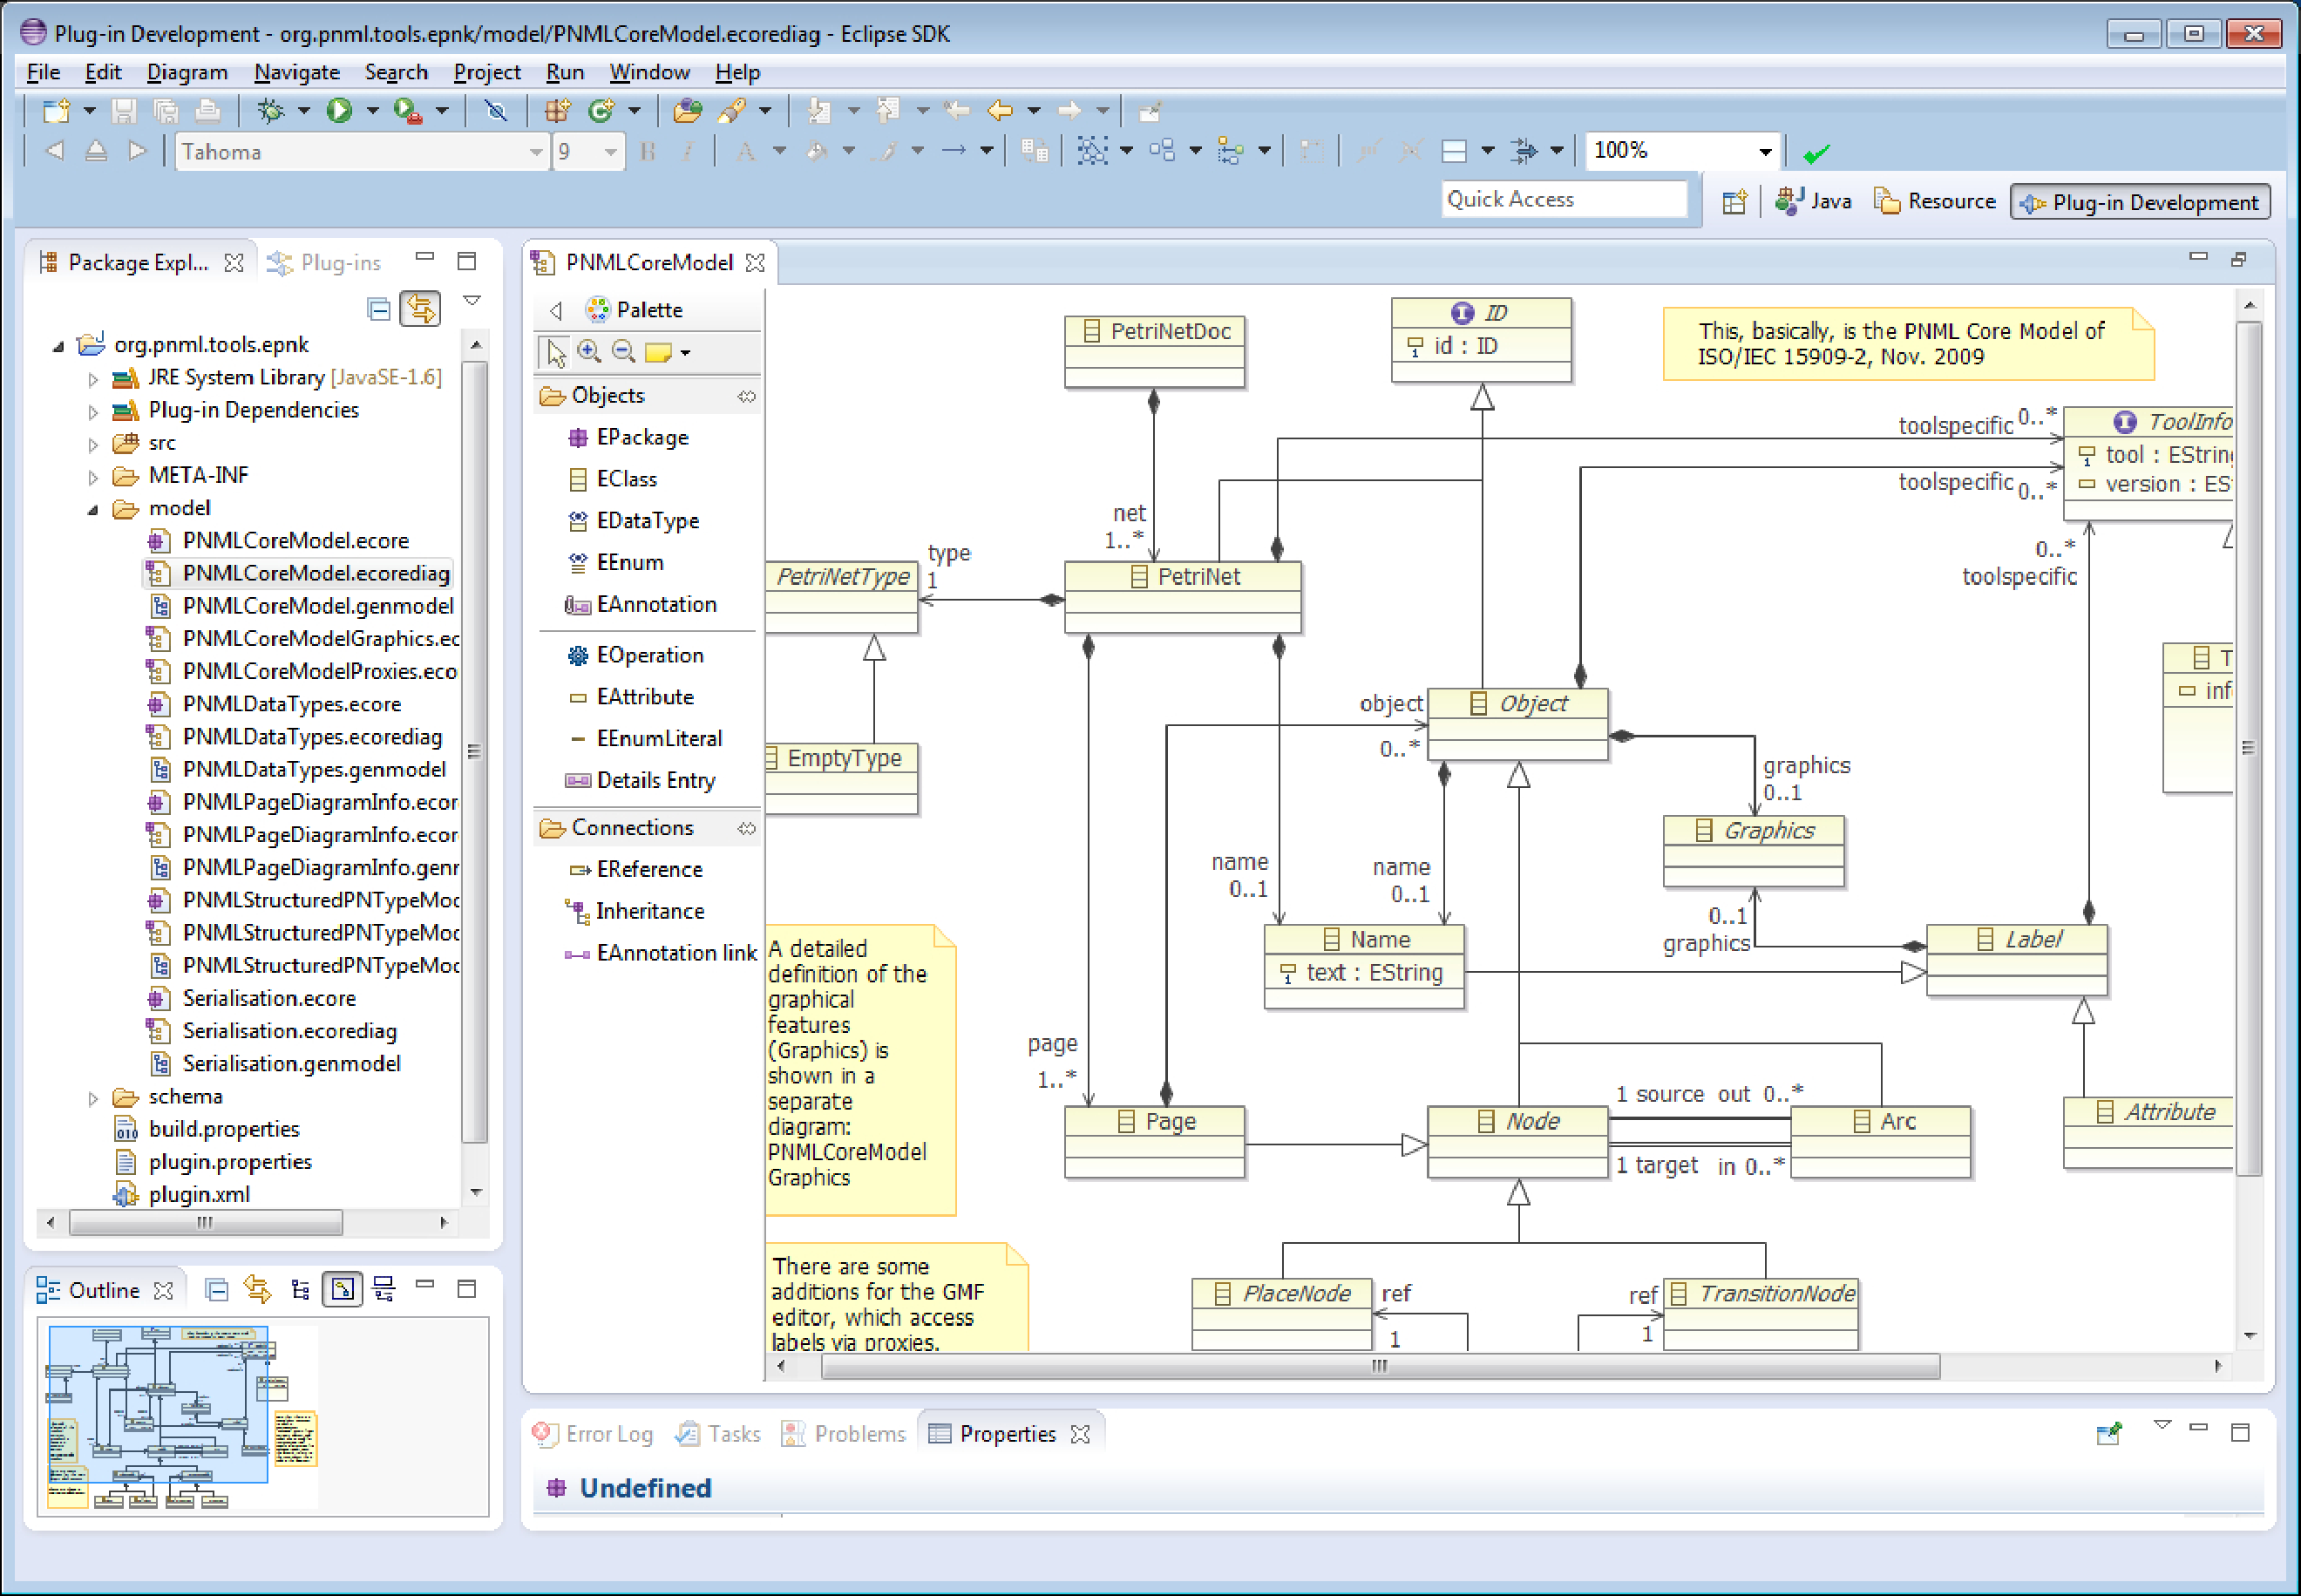
\includegraphics[scale=.28]{ePNK-IDE}}
  \caption{Developer's view with the ePNK PNML core model}
  \label{fig:ePNK-IDE}
\end{figure}


\section{The PNML core model in the ePNK}
\label{sec:ePNK-PNMLCoreModel}
% \index{PNML core model|(DEF}
\index{ePNK!PNML core model|(DEF}

For using the ePNK as a developer it is important to have a more
detailed understanding of the \emph{PNML core model} since the API
for accessing, navigating and modifying Petri nets is generated
from this model.  In Sect.~\ref{subsec:installingEcoreTools}, you have seen
already were to find and how to open the diagrams of the PNML core model
and some related diagrams. And when you start developing with the
ePNK, you will probably need to have a look into these diagrams
once in a while, in order to understand the details of the relation
between the different classes and concepts of PNML. 

In this section, we give an overview of the PNML core model of the
ePNK and discuss some of the differences to the PNML core model
of ISO/IEC~15909-2. As discussed in Sect.~\ref{subsec:PNMLcoremodel} already,
the PNML core model of the ePNK is slightly more general than the one of
ISO/IEC~15909-2:2011 \cite{ISO-IEC:15909-2-2011} (see Fig~\ref{fig:MetaModel}).
One of the main differences is the following: According to ISO/IEC~15909-2,
a page is not considered to be a node; in the ePNK, a page is considered to be
a node. This way, it is possible to define Petri net types in the ePNK that
allow arcs to be connected to pages (e.\,g.\ in order to define a Petri net
type that mimics substitution transitions of CPNs \cite{JeKr09}). Keeping
this in mind, might be particularly important, when defining the
constraints for arcs of net types (such as the ones for P/T-nets as
defined in Sect.~\ref{subsubsec:simplePNTDconstraints}), when you do
not want to allow to connect pages to other nodes with arcs.

The other differences of the PNML core model are a bit more technical
and will be discussed below. You might want to have a look at
Fig.~\ref{fig:MetaModel} of the PNML core model of ISO/IEC 15909-2:2011 
and at Fig.~\ref{fig:ePNK-IDE}, while we discuss the difference. For
more details, you can also open the Ecore diagrams in the project
{\tt org.pnml.tools.epnk} in your Eclipse workspace, provided you
have installed the legacy Ecore Diagram editor.

Most importantly, the {\tt type} of a Petri net is an attribute
of the class {\tt PetriNet} according to ISO/IEC~15909-2, whereas, in the
ePNK, it is a composition to a class that must inherit from the abstract class
{\tt PetriNetType}.%
  \index{ePNK!PetriNetType@{\tt PetriNetType}}
Instances of this class represent the Petri net type and will provide some
services to the ePNK to generically maintain the features of the respective
Petri net type. This is discussed in more detail in
Sect.~\ref{sec:adding-types}.
The PNML core model of the ePNK also provides one concrete class for a Petri net
type, which does not exists in ISO/IEC~15909-2:2011: {\tt EmptyType},%
  \index{ePNK!EmptyType@{\tt EmptyType}}
which represents a Petri net without any labels other than {\tt Names}.

In the ePNK, the {\tt source} and {\tt target} reference of the class
{\tt Arc} have a corresponding opposite reference from the {\sf Node} to its
{\tt out}-going and {\tt in}-coming {\tt Arc}s. These opposite references
are not serialized to the XML document, however, since this would not be
compliant with the PNML format. The opposite references will, however,
be restored when loading the Petri net. These opposite references are very
convenient when navigating between different elements of the net.

In turn, the ePNK does not have the class {\tt Annotation}%
  \index{ePNK!Annotation|DEF}
of ISO/IEC~15909-2, which represents those \emph{labels}%
  \index{Label|DEF}
that should be shown as graphical annotations
of the respective node or arc in the graphical editor. There exists a
class {\tt Attribute},%
  \index{ePNK!Attribute|DEF}
however, which represents those labels that
should be represented as properties of the respective element only,
but not as annotation in the graphical editor\footnote
 {By plugging in some graphical extensions, attributes can still have an effect
  on the graphical appearance of a Petri net.}%
. In the ePNK, all \emph{labels}%
  \index{ePNK!Label|DEF}
that are not attributes are considered to be
annotations. This has historical reasons, since the first version of the
ePNK did not support attributes at all; but, it also avoids making mistakes
in Petri net type definitions: it is impossible to define labels
that are neither attributes nor annotations.

At last, the PNML core model of the ePNK defines a separate interface {\tt ID},%
  \index{ePNK!ID|DEF}
which is used to unify all those elements that need a unique identifier in a
PNML document. All classes that must have such an identifier, implement the
interface {\tt ID} in the PNML core model of the ePNK. The reason for adding
the class {\tt ID} to the ePNK PNML core model is that, this way, the ePNK can
handle elements with an identifier in a uniform way; with the separate
id attribute for all elements as defined in the PNML core model of
ISO/IEC~15909-2, this would require much more effort.%
  \index{ePNK!PNML core model|)}%
% \index{PNML core model|)}
  
The attentive reader might also have noticed that the PNML core model of the
ePNK does not contain any OCL constraints, whereas the PNML core model
of ISO/IEC 15909-2 does. This, however, does not mean that the ePNK ignores
these constraints; in the ePNK, constraints are just added in a different way:
they are plugged in on top of the model. We will see examples of
how ePNK constraints are plugged in to the ePNK resp.\ to Eclipse later
(e.\,g.\ in Sect.~\ref{subsubsec:simplePNTDconstraints}).

\section{Adding functions}  
\label{sec:adding-functions}
\index{ePNK!Function|(DEF}

Next, we discuss how new functionality can be added to the ePNK. As discussed
earlier, there are two different ways of new adding new functionality to the
ePNK: \emph{Functions} take some net, possibly some user input, do some computing
and then report a result -- typically via some dialog window. After that, the function
is over and done with. The model checker from
Sect.~\ref{subsec:user:model-checker} is a typical example of a function.
By contrast, \emph{applications}%
  \index{ePNK!Application|DEF}
are started on a net; then, they show some feedback on top of the graphical
editor, the user can interact with the application, and the visual feedback
will be updated accordingly. Typically, an application finishes only
when the user explicitly terminates it. The simulator for high-level nets
of Sect.~\ref{subsec:user:hlpng-simulator} is a typical example
of an application.

In this section we, discuss the implementation of functions for the
ePNK. Basically, we use the standard mechanism of Eclipse to plug in
and start functions -- as \emph{views},%
  \index{Eclipse!View}
\emph{wizards},%
  \index{Eclipse!Wizard} 
\emph{actions},%
  \index{Eclipse!Action}
\emph{command handlers},%
  \index{Eclipse!Command handler}
\emph{jobs}%
  \index{Eclipse!Job}
or \emph{dialogs}.%
  \index{Eclipse!Dialog} 
In this manual, we explain the use of these concepts on the side, as far as they
are necessary. Since setting up jobs in a proper way can sometimes be a bit
tedious, the ePNK provides some utility classes that make programming jobs a
bit easier.

The focus of this section is on the use of the API of the ePNK that is
generated from the PNML core model and the Petri net type definitions
by the \emph{Eclipse Modeling Framework} (\emph{EMF}).%
  \index{EMF}
On the side, we point out some of the general principles of EMF and some
practical issues on working with EMF. For a more detailed introduction
to EMF, we refer to \cite{BSM06}. In this section, we do not only show
how to access, navigate and manipulate nets; we discuss also how
to open, create and write PNML files programmatically.

To this end, this section discusses how to plug in functionality into
the ePNK (or to Eclipse in general) in three different ways.
\begin{itemize}
\item Section~\ref{subsec:file-overview} shows how to implement a new
Eclipse view, which gives an overview of a PNML file that is selected in one of
the Eclipse resource explorer views. This section will also discuss how
top open and access the contents of a PNML file.

\item Section~\ref{subsect:multi-agent} shows how to implement a \emph{wizard}
for creating a PNML file (actually, the coded is based on a wizard that was
automatically created by the Eclipse ``new plug-in project wizard'').
This wizard creates a PNML file with a P/T-System that represents
a simple mutual exclusion algorithm for a number of agents -- where the
number can be selected by the user in one of the dialogs of the wizard.
The Petri net is split up to different pages, so that the Petri net for each
agent is contained in a separate page. In particular, we will discuss how
to create a PNML file, how to fill it with some contents and how to save it.

\item Section~\ref{subsec:tutorial-MC} shows how to implement a
simple pop-up menu on a selected Petri net (in the tree editor), which
starts a model checker, asking the user for some formulas to be checked,
and then checking the formulas on the net. Since model checking can take
quite some time, the model checker will run in the background and can
be aborted by the user. This uses Eclipse's concept of jobs. On the side, this
shows how to use some of Eclipse's user dialog functions.
\end{itemize}

In the end, Sect.~\ref{subsec:devloper:functitions:utilities} gives an overview
of the different functions of the ePNK (and the API generated from its EMF
model), some hints on how to work with this API in Eclipse and in EMF
general, as well as some additional ePNK utilities and helper classes that make it more
convenient to handle and access some of the information stored in a PNML document.
Experienced Eclipse and EMF developers, might want to start reading the overview
in Sect.~\ref{subsec:devloper:functitions:utilities} first, and come back
to Sect.~\ref{subsec:file-overview}--\ref{subsec:tutorial-MC} for some details
later.

\subsection{Accessing a PNML file and its contents: A file overview}
\label{subsec:file-overview}
\index{Eclipse!View|(DEF}

In this section, we discuss how to implement a new (and very simple)
Eclipse \emph{view}, that will give an overview of the contents of a PNML
file that is selected in the explorer. Figure~\ref{fig:file-overview-view} shows
a screenshot of the result. For the selected file ``hlpng-gmf.pnml''
in the ``Project Explorer'',  the ``ePNK File Overview'' at the
bottom left shows that the selected file is a Petri net document,
which contains 3 Petri nets, a high-level net, a P/T-net, and
an empty net; the type of a net is represented by its unique
URI. The name of the first net is ``A high-level next
example''; the other two nets do not have a name.

\begin{figure}[hbt!!]
  \centerline{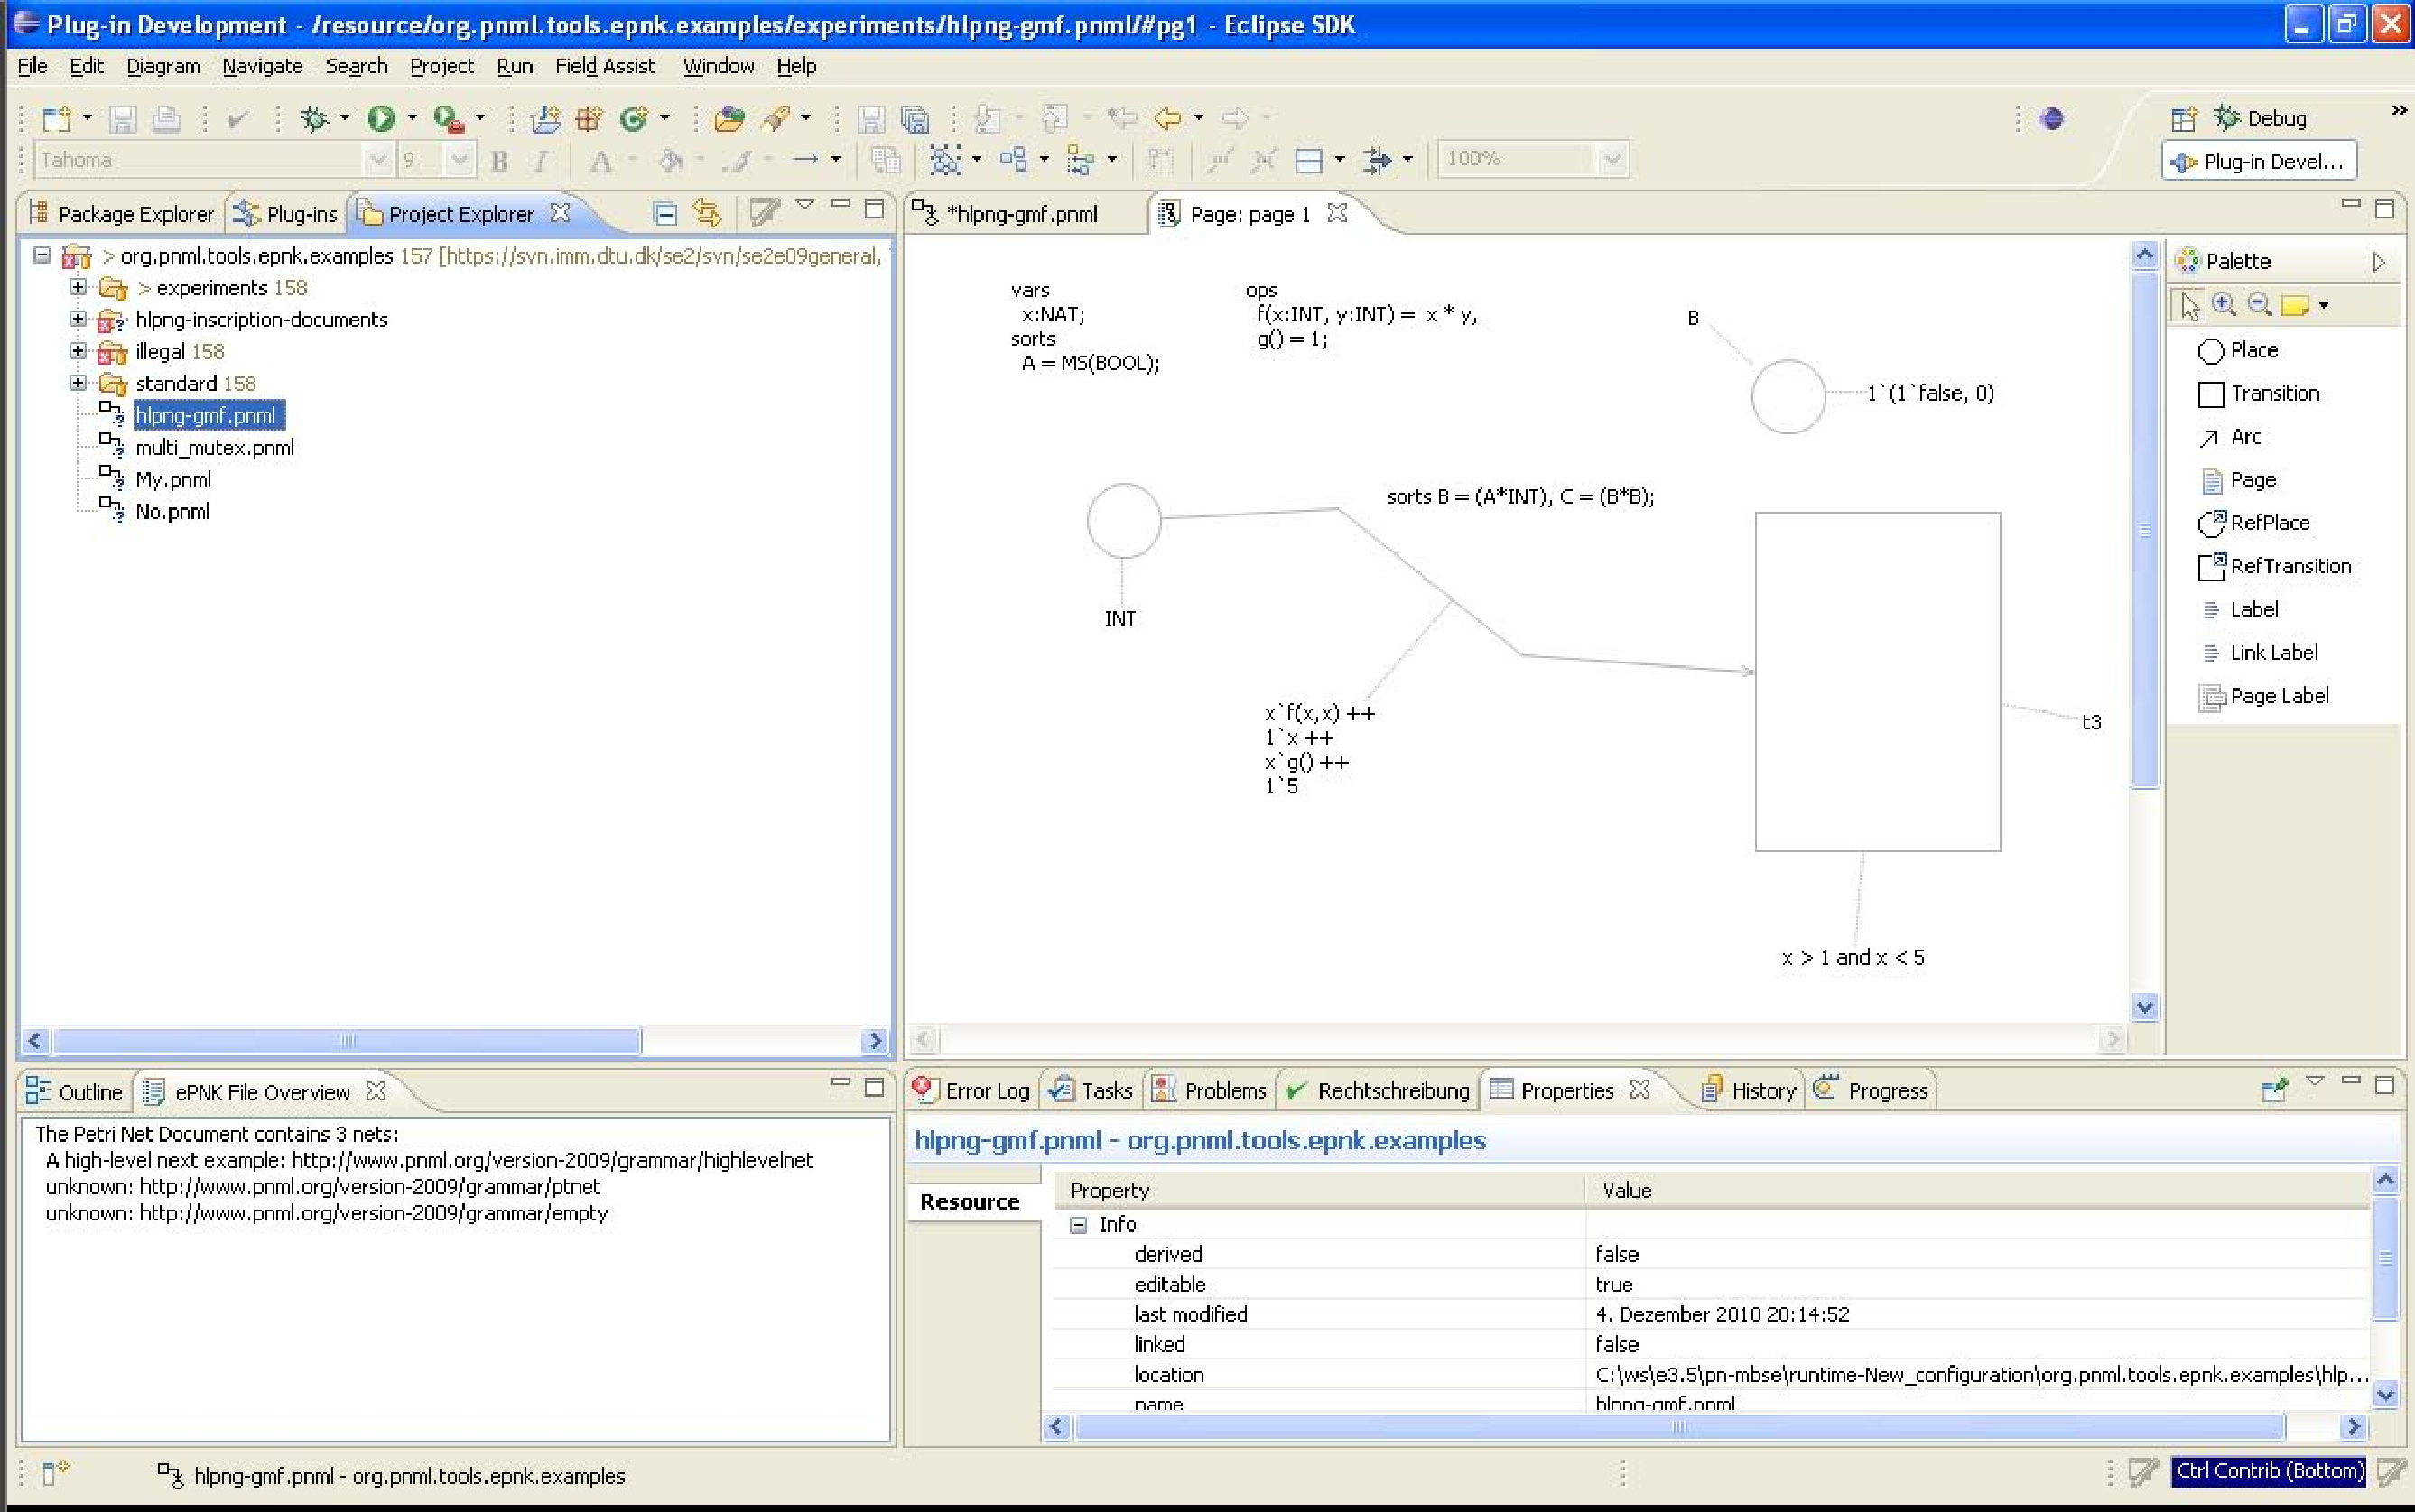
\includegraphics[scale=.27]{OverviewView}}
  \caption{The ePNK with the ``File Overview'' view}
  \label{fig:file-overview-view}
\end{figure}

This view and its functionality is implemented in the plug-in project
{\tt org.pnml.tools.epnk.functions.tutorial}. We go through this
project now\footnote
 {Remember that you can import the source code of that project to your
  development workspace from the ``Plug-ins'' view by selecting the
  project, right-clicking on it and then choosing ``Import As'' $\rightarrow$
  ``Source Project'' (see Sect.~\ref{sec:dev:import-ePNK}.}%
.  In addition to the overview view discussed above, this project also contains
the implementation of the wizard for creating a PNML document which will be
discussed later in Sect.~\ref{subsect:multi-agent}.

The implementation of the view is contained in a single Java class: {\tt
PNMLFileOverviewView} in the package
{\tt org\qnsep{}pnml\qnsep{}tools\qnsep{}epnk\qnsep{}functions\qnsep{}tutorial\qnsep{}overviewview}.
We briefly explain the general structure of this view class, an extract
of which is shown in Listing~\ref{lst:overview1};
%
\begin{figure}[htbp!]
\lstinputlisting[label=lst:overview1,tabsize=2,stringstyle=\small,%
caption={Class {\tt PNMLFileOverviewView}: Infrastructure}]%
  {code/PNMLFileOverviewView1.java}
\end{figure}
%
we deleted all imports, an attribute definition, and all comments; if needed
this information can be looked up in the source code. The class extends the Eclipse
{\tt ViewPart},%
  \index{Eclipse!ViewPart@{\tt ViewPart}|DEF}
which actually makes it an Eclipse view, and it implements the {\tt
ISelectionListener},%
  \index{Eclipse!ISelectionListener@{\tt ISelectionListener}|DEF}
which allows our view to obtain the information on the object that the user
has currently selected in the workbench.
Note that this class does not have an explicit constructor. The reason is that
the view will be set up via the {\tt createPartControl()} method:
In the first three lines of that method, a viewer (which represents the content
of that view) is initialized, and so-called providers will enable the view to
properly show the contents. Since these are standard Eclipse providers, we do
not discuss the details here.
In the last two lines of the {\tt createPartControl()} method,
our viewer registers itself with the Eclipse selection mechanism
as a \emph{selection listener}%
  \index{Eclipse!Selection listener}
and then creates the information that should be shown for the current user selection
by calling the {\tt selectionChanged()} method for the current selection. We will discuss
the respective method {\tt selectionChanged()} below.  Note that
there are two other methods. The {\tt setFocus()} methods forwards the
focus properly to the content of the view, once the view is focused.
More important is the {\tt dispose()} method: the implementation of
this method makes sure that our view removes itself as a selection
listener once it is disposed (which typically would happen when the
user decides to close the view).

Once the view has registered itself as a selection listener with
the Eclipse workbench, its {\tt selectionChanged()} method is
called whenever there is a change in the user's selection.
In the implementation of this method, the kind of the current
selection is analysed and it is checked whether the first
selected element is a file (i.\,e.\ whether it implements the
interface {\tt IFile}). If so, the method {\tt getOverviewInfo()}
for accessing the actual contents of the file and for computing
the contents of the overview is called; this produces an array of
Strings, which then will be set as the new contents of that view --
and, this way, shown to the user.%
\index{Eclipse!View|)}

The {\tt getOverviewInfo()} method is probably the most interesting
part here, since it shows how to open and access a PNML or a
PNX file (we do not even need to make a difference here). The implementation
of this method is shown in Listing~\ref{lst:overview2}.
%
\begin{figure}[htbp!]
\lstinputlisting[label=lst:overview2,%
tabsize=2,stringstyle=\small,%
caption={Class {\tt PNMLFileOverviewView}: Accessing the file}]%
  {code/PNMLFileOverviewView2.java}
\end{figure}
% 
Up to line 7, it is checked whether the file extension is
either ``pnml'' or ``pnx'' (the two file extensions, the ePNK uses
for storing Petri net files -- ``pnml'' represents files in PNML format, and
``pnx'' represents Petri net files in XMI, which we call PNX); then, the
path to that file is extracted and a URI of that path is created.
Actually, Eclipse provides also user dialogs and file dialogs that would
allow us to ask the user for a file name that would be returned as a URI; here
we used the selection mechanism and the file to get hold of some legal URI
of a PNML or PNX file. Therefore, the code that comes now, could be used at any
other point when a program wants to read and access some file, once we have a
String with the path to the file: This starts with creating a \emph{resource
set}%
  \index{Eclipse!Resource set|DEF}
and, within that resource set creating a \emph{resource}%
  \index{Eclipse!Resource|DEF}
with the given URI, which is the first parameter of the {\tt getResource()}%
  \index{EMF!getResource@{\tt getResource()}|DEF}
method; the second parameter indicates whether cross-references to other resources should be
resolved lazily or not (which is not relevant here). Note that, in EMF, a
resource or file should always be accessed (and created, see
Sect.~\ref{subsect:multi-agent} for more information) via a
resource set. After we successfully got the resource, we can obtain its contents
by the {\tt getContents()}%
  \index{EMF!getContents@{\tt getContents()}|DEF}
method which returns a list of its top-level objects
-- in case of PNML, this list should contain exactly one {\tt PetriNetDoc} object. 
Being defensive, we check whether the contents exists and whether its first element is an instance
of {\tt PetriNetDoc}. If so, we go systematically through all the contained nets, get
their names and their PNML types and add a String with that information to the
String array with the result. In the other cases, we return some error
messages. Note that we do not need to close the file, or do anything else after
we have obtained the information we need.

Let us have a closer look at how the contents of the Petri net
document is accessed, once we have obtained a {\tt PetriNetDoc}
object. For any reference and attribute of the \emph{PNML core model},%
  \index{PNML core model}
the ePNK API%
  \index{ePNK!API|DEF}
has corresponding \emph{getter}%
  \index{EMF!getter method|DEF}
 and \emph{setter methods}.%
  \index{EMF!setter method|DEF}
For example, if a class has an attribute {\tt name} of type {\tt String}, the
{\tt getName()} method will return the {\tt String} with that name, and with
{\tt setName()} we could set it -- but we do not change the net in this example.
For attributes and features with a multiplicity greater than one, this is
slightly different. For example, a {\tt PetriNetDoc} object can contain many nets;
therefore, {\tt getNet()} will return a list of nets, which we then can
iterate over to obtain the individual nets. And by adding a net
to this list, this Petri net would be added to the Petri net
document (see \ref{subsect:multi-agent} for examples).

As stated above, class {\tt PNMLFileOverviewView}
implements the ``ePNK File Overview'' as we have seen it in
Fig.~\ref{fig:file-overview-view}. But, it is not enough to just implement
this class; it would not show up in Eclipse, because Eclipse would
not know that it exists. In order to make the view known to
Eclipse, we need to define it as an \emph{extension}:%
  \index{Eclipse!Extension|DEF}
This is done in the project's ``plugin.xml''%
  \index{Eclipse!pluginxml@{\tt plugin.xml}|DEF}
file. Double clicking on the
``plugin.xml'' file, will give you a convenient editor for defining and	editing
the extensions you want to define. Explaining the actual extensions is a bit
easier with the XML fragment that is produced by this editor. The
fragment relevant for our overview view is shown in Listing~\ref{lst:overview-plugin}.
%
\begin{figure}[htbp!]
\lstinputlisting[language=XML,label=lst:overview-plugin,tabsize=2,stringstyle=\small,%
caption={Defining the overview view extension in ``plugin.xml''}]%
  {code/overview-plugin.xml}
\end{figure}
% 
It says that we contribute our \emph{extension}%
  \index{Eclipse!Extension|DEF}
to the Eclipse \emph{extension point}%
  \index{Eclipse!Extension point|DEF}
{\tt org.eclipse.ui.views}, which is a
new Eclipse view. The category defines where and under which category
the new view can be found, when the user wants to open it
via the Eclipse ``Show View'' menu.
We define a category specifically for the ePNK and then define the actual view
referring to this category.
The attributes of the view say that a view of this kind can
at most be open once, that it uses the above category, and refer to the
class which actually implements it: {\tt PNMLFileOverviewView};
and the attributes define an icon (used in the tab of that view) and 
a name for that view.

Note that in order to access some of the classes such as {\tt Resource},
{\tt Resource\optsep{}Set}, and some of the ePNK classes like {\tt PetriNetDoc},
{\tt PetriNet}, etc.\ in the implementation of the view, we would also need to
define dependencies to the plug-in projects by which they are provided: If you
open the file ``plugin.xml'', you will find these projects in the tab ``Dependencies''.  But
this is a more technical issue, which we do not go into the details.

Now, you could start the runtime workbench of Eclipse; from there, you could open the
``ePNK File Overview'' by ``Window''$\rightarrow$ ``Show
View''$\rightarrow$ ``Other...'' and then selecting ``ePNK File Overview''
in the category ``ePNK''. This will show the view in the workspace as shown
in Fig.~\ref{fig:file-overview-view}. Whenever the user selects some
PNML or PNX file in the package explorer, this view will show an overview
of the contents of the selected file. Since this plug-in project is deployed
with the ePNK 1.0.0 already, it is of course not even necessary to start the
runtime workbench -- the view is already there in the development workbench,
once the ePNK is installed.


\subsection{Writing PNML files: Generating multi-agent mutex}
\label{subsect:multi-agent}

Next, we discuss how to create new PNML files and how to fill them
with some contents.
In typical applications, the contents might come from a file in a format of
another Petri net tool, which should be converted to PNML. In our example,
however, we programmatically generate a Petri net: my favourite semaphore mutex
example, which was used in Sect.~\ref{subsec:user:model-checker} as an
example for model checking already.
To make things slightly more interesting, the number of agents competing for the
semaphore is a parameter.  This function is implemented as an Eclipse
\emph{wizard}%
  \index{Eclipse!Wizard|DEF}
and it was implemented by creating a new file wizard for PNML files
automatically by the Eclipse ``New Plug Project'' wizard choosing the
``custom plug-in wizard'' with the choice of the ``New File Wizard'' in
the ``Template Selection'' dialog. But, this does not need to bother you too
much. If you are interested in the manual changes made to the automatically
generated code, you will find all the manual changes in the two classes
in the package {\tt org.pnml.tools.epnk.functions.tutorials.wizards} enclosed
by comments like {\tt // eki: ... }. These packages are contained in the
same plug-in project, 
{\tt org.pnml.tools.epnk.functions.tutorials},
as discussed in Sect.~\ref{subsec:file-overview} already.

In the rest of this section, we focus on the explanation of the parts of the
implementation that are concerned with the creation of the file and its contets.
This functionality is implemented in the method {\tt createPNMLFile()} of
the class {\tt MultiAgentMutexNetWizard}, which is shown in
List.~\ref{lst:createFile}. The parameter {\tt path} is a String representation
of a path to the file that should be created. The parameter {\tt number} is the
number of agents that should be created in the mutex net that will be generated.  

Creating the Petri net programmatically is quite straightforward, but code
intensive. Therefore, we have split up the creation process into several parts
for the different elements, which will be discussed top-down from creating
the document, the net, its pages, and the places, transitions, reference
places, and arcs on them. We discuss these methods one after the other --
and omit some boring ones in the end (you can find all details in the
source code).
%
\begin{figure}[bp!] % [htbp!]
\lstinputlisting[label=lst:createFile,tabsize=2,stringstyle=\small,%
caption={Method {\tt createPNMLFile(String path, int number)}}]%
  {code/MultiAgentMutexNetWizard1.java}
\end{figure}
%
Listing~\ref{lst:createFile} shows the method that creates the
file: First, it calls the method {\tt createPetriNetDoc()} that creates the
Petri net document, which is discussed later. This is the contents of the file
that we want to write. Then, we convert the path into a URI. Then, we create a
resource set%
  \index{Eclipse!Resource set|DEF}
-- from which the resource (the file) is create. Surprisingly
enough, this is already all we need to do. At this point, we can add the
contents to the resource. Note that it does not even matter whether the
resource is a PNML file or a PNX file -- Eclipse will, dependent on the file
extension, chose the right implementation of the resource so that either a PNML
file or a PNX file is written once we save the resource in the end. But, we
configured the wizard in such a way that the user can chose only
the ``pnml'' extension.

Adding the contents follows the same principle that we have discussed already.
With {\tt getContents()}%
  \index{EMF!getContents@{\tt getContents}|DEF}
we get a list of EMF objects (which would be empty,
since the resource was newly created right now); then we add the Petri net
document to this list. The only thing left is to save the resource, which is
done by calling the {\tt save()}%
  \index{EMF!save@{\tt save()}|DEF}
method. Note that the save method has a
parameter, that could be used to configure the way a file is saved. 
But, {\tt null} is fine here -- and you should only change this, if you know
exactly what you are doing.

\index{ePNK!API|(DEF}%
Let us dive a bit deeper into the method {\tt createPetriNetDoc()}, which
takes one parameter only -- the number of agents.
%
\begin{figure}[htbp!]
\lstinputlisting[label=lst:createFile2,tabsize=2,stringstyle=\small,%
caption={Method {\tt createPetriNetDoc(int number)}}]%
  {code/MultiAgentMutexNetWizard2.java}
\end{figure}
%
This method is shown in Listing~\ref{lst:createFile2}. In the
second line, a new Petri net document is created. Note that this is not done
using Java's {\tt new} construct. Rather, the \emph{factory}%
  \index{EMF!Factory|DEF}
for the PNML core model is obtained by
{\tt Pnmlcoremodel\optsep{}Factory\qnsep{}eINSTANCE},%
  \index{ePNK!PnmlcoremodelFactory@{\tt PnmlcoremodelFactory}|DEF}
which is then used for creating a new {\tt PetriNeyDoc} object. It is part of the
EMF philosophy that clients using the generated code should not know anything about
the actual implementation of classes. And EMF strongly recommends to create
new objects only via these factories.
Note that also the new net is not directly created; it is created by
using the ePNK's type registry {\tt PetriNetTypeExtensions},%
  \index{ePNK!PetriNetTypeExtensions@{\tt PetriNetTypeExtensions}|DEF}
  \index{ePNK!Type registry|DEF}
which creates the Petri net with the correct type from its URI. Note that the
net will be {\tt null}, if no net type is registered for the respective URI.

After creating the net, its id is set by the {\tt setId()} method. Note that this
could be any string, but it is our responsibility to make sure that all ids
are different (if we chose to create the ids programmatically). Then, the net is
added to the list of nets of that document: to this end, we get
the list of all nets of the document via the {\tt getNet()} method on which we
call the {\tt add()} method. There is no way to directly add a net to
a document. 

After that, a name label is created, its text value is set, and the
name label is added to the net. 

Next, a new page is created by calling a separate method, which is added
to the list of pages of the net, and the place semaphore is created
as the single object on this page. To this end, we use the
{\tt createPlace()} method. 

In the for-loop at the end of the method, for each agent, there
will be created one page with the net for each agent.

All the other methods follow the same principles, and there  is
not too much interesting to see in them.
%
\begin{figure}[htbp!]
\lstinputlisting[label=lst:createFile3,tabsize=2,stringstyle=\small,%
caption={Method {\tt createAgentPage()}}]%
  {code/MultiAgentMutexNetWizard3.java}
\end{figure}
% 
Therefore, we finish with discussing the method {\tt  createAgentPage()},
which is shown in Listing~\ref{lst:createFile3}. This method
creates 3 places, one reference place (referring to the semaphore
that was created on the first page above), 3 transitions, and 8 arcs.
What makes this method a bit more interesting is the graphical
information that is added to the arcs: some intermediate point,
which makes the net look a bit nicer. If you have a closer look
at the {\tt createTransition()}, {\tt createPlace()}, and  {\tt createRefPlace()}
you will find similar constructs for defining the position and size
of the nodes, and the position of the labels associated with them.
But this is straightforward and follows the exact principles
of ISO/IEC~15909-2 (see \cite{HKea09}). Note that, if a reference
pace is created, the place it refers to needs to be set by
{\tt setRef()}; therefore, we need to pass the the place {\tt semaphor}
to the {\tt createRefPlace()} method as a parameter.

Once the implementation
of the wizard class is finished, it must be made know to Eclipse: it must be
plugged in via the ``plugin.xml''. But, we do not discuss this here since
this is similar to plugging in a view (have a look
into the ``plugin.xml'', if you are interested).

In the runtime workbench (or a version of the ePNK in which this plug-in
is installed already), you could invoke this function as follows: Go to the
resource explorer -- or any other explorer -- of the workbench, press
the right mouse button and select ``New''$\rightarrow$``Other...'',
select ``Multi-agent Mutex Net Wizard'' in the category ``ePNK''. Then,
a dialog opens in which you can choose a folder\footnote
  {If you have selected exactly one folder when you invoke the
   wizard, the fields of this dialog will be pre-set.}
(``container'') in which this file should be created, a ``file name'' (which
must have extension ``pnml''), and the number of agents. Note that, normally,
the file creation wizard would overwrite existing files. This ``multi-agent''
wizard, however, was modified in such a way that existing files won't be
overwritten accidentally.%
  \index{ePNK!API|)}

\subsection{Long-running functions: A model checker}
\label{subsec:tutorial-MC}
\index{Job|(DEF}

In this section, we discuss the implementation of a model checker for P/T-Nets,
which, actually, are interpreted as EN-Systems here. The model-checker is based
on a simple library for symbolic model checking that was developed for
teaching purposes: \emph{Model Checking in Education} (\emph{MCiE})\footnote{
see \url{http://www2.cs.uni-paderborn.de/cs/kindler/Lehre/MCiE/}}. This MCiE
library is deployed as part of the ePNK tutorials.

In this developers' guide, we will not go into the details of model checking
and its theoretical foundation, since this is not the point of this tutorial
at all. For more information on model checking, we refer to a standard text book
on model checking~\cite{CGP99}. The point of this tutorial is to show how some
function can be installed as a \emph{pop-up} menu with an \emph{action} on a
Petri net that is open in the tree editor\footnote
  {Note the extension points for pop-up menus and actions are deprecated
   since Eclipse~4.2. But, they still work -- eventually, this will be adjusted
   by using Eclipse commands and handlers.}%
. Model checking can actually be quite computation intensive and
could take quite some time; therefore, we need to make sure that the actual
model checking action does not block the graphical user interface of Eclipse
while the model checker is running. Eclipse provides \emph{jobs} for this
purpose, which allow to run tasks (or jobs) in the background.
The ePNK provides some convenience classes that make it a bit easier to set up
and start jobs, which are running in the background -- and provide a possibility
to show a result in a dialog, once the job is finished.

The model checking functionality is implemented in the plug-in project
{\tt org\qnsep{}pnml\qnsep{}epnk\qnsep{}functions\qnsep{}modelchecking}. Like the other projects,
you can import the source code of this project to your workspace via
the Eclipse ``Plug-ins'' view and the ``Import As'' $\rightarrow$ ``Source
Project'' menu. The actual model checker is implemented in
the class {\tt ModelcheckingJob} in package
{\tt org\qnsep{}pnml\qnsep{}epnk\qnsep{}functions\qnsep{}modelchecking\qnsep{}action}.
The action initiating the model checking job is
{\tt Modelchecking\optsep{}Action} in the same package.

Since the class {\tt ModelcheckingAction} and the way it is integrated to
the ePNK is quite simple, we start with explaining this one first. It is shown
in Listing~\ref{lst:mc-action}.
%
\begin{figure}[htbp!]
\lstinputlisting[label=lst:mc-action,tabsize=2,stringstyle=\small,%
caption={The action class {\tt ModelcheckingAction}}]%
{code/ModelcheckingAction.java}
\end{figure}
%
This class extends the {\tt AbstractEPNKAction},%
   \index{ePNK!AbstractEPNKAction@{\tt AbstractEPNKAction}|DEF}
which is an ePNK convenience class that makes it easy to add a new action,
which initiates a job. The class {\tt AbstractEPNKAction}
overrides two methods: {\tt isEnabled()} and {\tt createJob()}. The method
{\tt isEnabled()} checks whether the action is applicable for the selected Petri
net. In our example, it checks whether the Petri net has a type and whether this type
is {\tt PTNet}. The other method {\tt  createJob()} creates the actual job,
which is an instance of class {\tt ModelcheckingJob} with a Petri net and a
defaultInput (a default formula for the user dialog in our case). This class
extends the ePNK's convenience class {\tt AbstractEPNKJob}%
  \index{ePNK!AbstractEPNKJob@{\tt AbstractEPNKJob}|DEF}
and will be discussed later.

In order to make the action {\tt ModelcheckingAction} know to Eclipse
and appear in the popup menu in the ``ePNK'' category, we need to define
an extension. Listing~\ref{lst:mc-plugin} shows the part of
the ``plugin.xml'' file that defines this extension (with some ellipses).
%
\begin{figure}[tbp!] %[htbp!]
\lstinputlisting[language=XML,label=lst:mc-plugin,tabsize=2,stringstyle=\small,%
caption={Defining the popup action for the model checking action}]%
{code/mc-plugin.xml}
\end{figure}

At last, we have a look at the class {\tt ModelcheckingJob}, which
is implementing the user dialogs (asking the user for temporal formulas),
converting the Petri net into ROBDDs, doing the actual model checking,
and showing the result to the user again. In addition to the constructor,
we need to implement (override) the following methods of
{\tt AbstractEPNKJob}:%
  \index{ePNK!AbstractEPNKJob@{\tt AbstractEPNKJob}|DEF}
{\tt prepare()}, {\tt getInput()}, {\tt run()}, {\tt showResult()}, and {\tt
canceling()}. Below we explain the implementation of the constructor and the
methods:
\begin{description}
\item[Constructor:] Sets up all the data structures needed during the job;
    typically, this will be storing the default input. In our model checker
    example, we also set up some mappings, for mapping places of the
    Petri net to variables of the MCiE library, and mappings from transitions    
    to formulas defining their behaviour, and some other information.
    The code of the constructor is shown in Listing~\ref{lst:mc-constructor}.
\begin{figure}[tbp!] %[htbp!]
\lstinputlisting[label=lst:mc-constructor,tabsize=2,stringstyle=\small,%
caption={The constructor of {\tt ModelcheckingJob}}]%
{code/ModelcheckingJob1.java}
\end{figure}

\item[{\tt prepare()}:] This method is handling the user dialogs before the
    actual job starts. In our case, it asks the user for some CTL-formulas;
    it also allows the user to correct the input, if the formulas are
    syntactically incorrect -- or to abort the action. The code for this
    user dialog is shown in Listing~\ref{lst:mc-dialog}. Since this is
    standard Eclipse programming, we do not go into the details of
    this part here. The only relevant part for the ePNK is that the
    job will not be continued, if the {\tt prepare()} method returns false --
    in the implementation of the model checking job, this is done, when
    the user presses cancel in one of the dialogs (line 11/12 and line 33/34).
  
\begin{figure}[htbp!]
\lstinputlisting[label=lst:mc-dialog,tabsize=2,stringstyle=\small,%
caption={The user dialog of the {\tt prepare()} method}]%
{code/ModelcheckingJob2.java}
\end{figure}    

    In our model checking job, the {\tt prepare()} method will try to convert
    the Petri net into formulas defining the behaviour of the transitions
    and the initial marking. And on the way, it will be checked whether there
    are duplicate names of places, so that a warning can be issued.   
    Listing~\ref{lst:mc-prepare} shows the part of the {\tt prepare()} method
    converting the initial marking into a state formula.
\begin{figure}[tbp!] %[htbp!]
\lstinputlisting[label=lst:mc-prepare,tabsize=2,stringstyle=\small,%
caption={Building the formula for the initial marking (in {\tt prepare()})}]%
{code/ModelcheckingJob3.java}
\end{figure}
    The basic idea is that, in this formula, a variable corresponding to the
    place occurs exactly once. It occurs negated, if the place is not marked
    and it occurs without negation, if the place is marked (with at least one
    token\footnote
      {Remember that we abuse P/T-Nets for representing EN-Systems.}). 
    All these negated and un-negated variables are connected by boolean
    and-operations as formulas represented in MCiE's data structure.
    What is more interesting here is that the ePNK provides a way to access a net
    that consist of pages with reference nodes in a flattened way. This
    convenience class of the ePNK is called {\tt FlatAccess};%
       \index{ePNK!FlatAccess@{\tt FlatAccess}|DEF} 
    its static method {\tt getFlatAccess()} called with a parameter of a
    Petri net of any type creates a \emph{flat access object} for that net
    (called {\tt flat} in our case).
    This flat access object can be used to obtain all places of the net,
    independently of the  pages they occur on. Likewise, the
    flat access object provides methods to access all the transitions and to get all
    the input and output arcs of a place or transition (including the ones of
    the reference nodes referring to them). This way, it is easy to obtain the
    pre- and post-sets, without being bothered with the page structure. For some
    more examples of the use of these methods, you can have a look into the
    code that converts transitions into formulas, which however is not
    discussed here.
    
    Note that creating a flat access object is quite computation intensive;
    therefore, the static method {\tt getFlatAccess()} for creating a
    flat access object\footnote
      {Note that in earlier versions of the ePNK, the flat access object
       was created by a constructor. This constructor is deprecated now,
       and should no longer be used; but, it is still there, so that
       older code should still be working. It is strongly recommended,
       to replace the use of the constructor, though.}
    will create only one  flat access object for each net. But, the
    flat access object becomes invalid, when the underlying Petri net changes.
    The flat access object can, therefore, also be used to notify an
    application that the underlying net has changed. But, we do not discuss
    the details here.
    
    The last part of the prepare method, is converting the formulas into
    ROBDD-representation and creating a transition system out of these formulas.
    This is shown in Listing~\ref{lst:mc-prepare2}.
    Again, this is specific to MCiE. But, there are two parts that are
    important for the {\tt prepare()} method in general: With {\tt 
    this.setName()}, we can give the job a specific name, which is used in
    Eclipse's jobs view. In our example, we say that it is a model checking job,
    add the name of the net and the formula which the user entered. The last
    important part is that the  {\tt prepare()} method returns {\tt true} in order to
    indicate that the preparation successfully terminated, and the actual
    job can be run (in the background) now.
\begin{figure}[htbp!]
\lstinputlisting[label=lst:mc-prepare2,tabsize=2,stringstyle=\small,%
caption={Finishing the {\tt prepare()} method}]%
{code/ModelcheckingJob4.java}
\end{figure}

    Note that all computations in the {\tt prepare()} method should run fast.
    Computations that are time-consuming should be implemented in the {\tt
    run()} method, which will be run in a separate thread in the background.

\item[{\tt getInput()}] This method is called by the action, to get and store
     as default for the next call, the user input. In our case, the formula
     that was entered by the user during the prepare phase (in its String
     representation as entered by the user) is returned.
     
\item[{\tt run()}] This method implements the part of the job that will be run
     in the background -- and typically contains the computation intensive
     parts. In our case, this is the actual model checking task.
     The implementation of the method is actually quite simple (most of the
     programming work lies in the preparation and the MCiE framework).
     It is shown in Listing~\ref{lst:mc-run}.
\begin{figure}[tbp!] % [htbp!]
\lstinputlisting[label=lst:mc-run,tabsize=2,stringstyle=\small,%
caption={The {\tt run()} method}]%
{code/ModelcheckingJob-run.java}
\end{figure}
     Still, it is the most computation intensive part, which is why we are using
     the job to run it in the background. Note that, at the end of this method,
     we also prepare the {\tt result} already in a String that will be shown to the
     user. But, there must not be any user dialog in the {\tt run()} method
     itself, since this method is run in a separate thread in the background --
     and user dialogs would require to be called from a dedicated GUI thread. 

\item[{\tt showResult()}] This is the method that will be called for showing
     the result to the user. And, the infrastructure from {\tt AbstractEPNKJob}
     will make sure that it will be called from the dedicated GUI thread again.
     Therefore, we can use all Eclipse dialogs for showing the result. 
     Listing~\ref{lst:mc-showresult} shows the implementation of this method.
     The result String, which was prepared during the {\tt run} method is
     shown to the user by initiating an information dialog.
\begin{figure}[tbp!] %[htbp!]
\lstinputlisting[label=lst:mc-showresult,tabsize=2,stringstyle=\small,%
caption={Code for showing the final result}]%
{code/ModelcheckingJob-showResult.java}
\end{figure}

\item[{\tt canceling()}] This method is a call-back mechanism that allows
     Eclipse -- typically triggered by the end user -- to abort a job that is
     running in the background.
     In the case of computation intensive jobs, to abort the
     computation and not to let that thread continue in the background is very
     important; otherwise this thread would consume all the computation power
     until it finishes on its own -- which could take extremely long. Therefore,
     MCiE provides a mechanism for aborting model checking operations on some
     model, by invoking {\tt abort()} on the underlying transition system on
     which the model checking is done. Our
     implementation of the {\tt canceling()} method invokes this {\tt abort()}
     method to actually terminate the model checking -- possibly with some
     delay. This is shown in Listing~\ref{lst:mc-cancelling}, where {\tt
     transitionsystem} is the one that was constructed before in the {\tt
     prepare} method and on which the model checking is done. This will actually
     cause the model checker -- the thread in which the computation is
     running -- to throw some exception at some
     point of its computation in the {\tt isValid()} method; this will stop
     the complete thread, since the exception is not caught.
%
\begin{figure}[tbp!] % [htbp!]
\lstinputlisting[label=lst:mc-cancelling,tabsize=2,stringstyle=\small,%
caption={Code for aborting the model checking job}]%
{code/ModelcheckingJob-cancelling.java}  
\end{figure}
\end{description}

Together, the classes {\tt ModelcheckingAction} and {\tt ModelcheckingJob},
plugged in via the ``plugin.xml'' implement a simple, but complete model
checker. If the model checking project was not already part of the ePNK, you
would start the runtime workbench, and would have the model checker
available there.  Section~\ref{subsec:user:model-checker} of the
Users' Guide had explained already how to use this model checker.%
  \index{Job|)}%
  \index{ePNK!Function|)}

\subsection{Overview of the ePNK API}
\label{subsec:devloper:functitions:utilities}

The previous sections have given an idea of how the ePNK and its
API can be used to access and modify Petri nets for implementing some
functions on Petri nets. It also showed how to plug in these functions
to the ePNK -- or actually to Eclipse. But, these examples just scratch
the surface. In this section, we give an overview were to find and look
up things in the API of the ePNK and how to use this API in the context
of Eclipse and EMF. Most of these things, are actually not specific to
the ePNK, but specific to Eclipse and EMF, and could be read up on
in the many Eclipse publications (e.\,g. \cite{BSM06,ClRu08,Gro09}).
Anyway, we briefly mention or point to some of the relevant concepts
here, in order to avoid some unpleasant surprises.

\subsubsection{Eclipse and EMF}
\label{subsubsec:ePNK:API:EMF}

We start with giving an overview of the code that is generated\footnote
  {EMF provides many features to configure and change the way the code
   is generated from a model. Here, we discuss only the standard settings,
   which -- with some few exceptions -- are used for all models of the ePNK.}
from Ecore models, which was also briefly discussed in
Sect.~\ref{subsec:file-overview} already. All models used in the ePNK are
\emph{Ecore models},%
  \index{EMF!Ecore model|DEF}
which are an implementation of the \emph{Meta Object Facility} (\emph{MOF})
\cite{MOF05}. For the purpose of this manual\footnote {We do not bother to go into the details of the MOF-levels and into the
   motivation behind MOF. See \cite{Kin09c} for an brief introduction and
   overview.}%
, an Ecore model can considered to be a simplified version of a UML class
diagram. Note that, in Ecore models, the concept that represents a UML
association is called \emph{references}%
  \index{EMF!Reference|DEF}
-- and in the case of a bi-directional association, a pair of two
\emph{opposite} references.


\index{EMF!API (generated from model)|(DEF}%  
The \emph{Eclipse Modeling Framework} (\emph{EMF}) \cite{BSM06} allows us to
generate Java code from these models, which provides \emph{getter}%
  \index{EMF!getter method|DEF}
and \emph{setters methods}%
  \index{EMF!setter method|DEF}
for all the attributes and references. And there will be a lot of code behind
the scenes for loading and saving models, and for notifying some observers when
changes are made. Actually, in the generated code, each class of an Ecore model
is represented by a Java interface and a Java class implementing this interface;
the interfaces and implementations reside in two different Java packages --
where typically the package name with the implementing classes ends with a segment called ``impl'' and also
the name of the implementing Java class will end with ``Impl''. Normally, developers that want to access
model elements, would use the interfaces only. For attributes and references
with multiplicities 1 or 1..0, the generated API and the use of the generated
setter and getter methods is straightforward\footnote 
  {There is a minor, but sometimes confusing twist when an attribute is
   of type boolean: in that case, the getter method actually starts with
   ``is''.}%
.  In case of multiplicity *, you will find that there are no setter methods
for the respective attribute or reference at all; there will be a getter method,
which returns a collection. In order to add or remove an element to or from the
attribute or reference, you would obtain this list by the getter methods, and
then add or remove something from the collection by the respective methods of
collections. Note that this collection is attached to the object, and it is
crucial that you do not use it for other purposes.  

As explained above, the package with the Java classes that implement the
Java interface of the model should typically not be used directly by other
developers. This also applies to the constructor (which normally is protected).
If a developer wants to create an instance of some class, this should be
done via a \emph{factory}%
  \index{EMF!Factory|DEF}
for the model, which can be found in the same Java package as the generated Java
interfaces of the model. This factory class is typically called {\tt
XXXFactory}, where  {\tt XXX} is the name of the package; the singleton
instance of this class can be accessed by an attribute {\tt eINSTANCE}.
For each class of the model, this Factory provides a method for creating
a new instance of the respective class.%
  \index{EMF!API (generated from model)|)}  


Note that all\footnote
  {Remember that we discuss the standard configuration of EMF only.}
Java classes that are generated as implementations for classes from the Ecore
model inherit from the class {\tt EObject}%
  \index{EMF!EObject@{\tt EObject}|DEF}
of the EMF Framework. The class {\tt EObject} provides a lot of functionality
behind the scenes and also some convenience methods. For example, it allows another object
to register with it as a listener, so that the other object is notified
about any changes of its attributes and references, and even some other events.
But, we do not go into these details here. One of the convenience methods
is to obtain an iterator of all its directly and indirectly contained
elements (indicated by compositions in the Ecore model): {\tt eAllContents()}.%
  \index{EMF!eAllContents@{\tt eAllContents()}|DEF}
All the methods of the {\tt EObject} start with the letter ``e''. We
cannot discuss them here; for example, there are methods for reflectively
finding out which model class this object represents {\tt eClass()};%
  \index{EMF!eClass@{\tt eClass()}|DEF}
there is a method {\tt eContainer()}%
  \index{EMF!eContainer@{\tt eContainer()}|DEF}
to obtain the object in which this object is directly contained; there are
methods to find out which features this object has, and to change them.

Note that {\tt EObject} has a method {\tt eResource()},%
  \index{EMF!eResource@{\tt eResource()}|DEF}
which returns the resource (file)%
  \index{Eclipse!Resource|DEF}
in which the object is contained -- if it is associated with
a file already. Resources are important, when your want to load and save
models to a file, and when they are loaded and edited in an editor. Actually,
a resource is typically contained in a \emph{resource set},%
  \index{Eclipse!Resource set|DEF}
which is responsible for maintaining different resources that refer to each
other -- and for loading and saving them together so that the links between them
remain consistent. For a resource, the resource set it is contained in can be
obtained by method {\tt getResourceSet()}.%
  \index{EMF!getResourceSet@{\tt getResourceSet()}|DEF}
In turn, resources can and should be created from a resource set, which will
make sure that the correct type of resource is used for the respective file type We
have seen two examples of that: in the file overview (Sect.~\ref{subsec:file-overview}),
the resource set and resource was used to open a selected PNML file; in the
``multi-agent mutex wizard'' (Sect.~\ref{subsect:multi-agent}), the resource set was used
to create a new PNML file. Note that, once you have a resource, its contents
can be obtained by the method {\tt getContents()},%
  \index{EMF!getContents@{\tt getContents()}|DEF}
which returns a list of {\tt EObjects}; which can be used to access the element,
but also to add new elements. The {\tt save()}%
  \index{EMF!save@ {\tt save()}|DEF}
method of the resource can be used to save the current contents of the resource
to the file.

Note that the only example where we actually change (or create) a Petri net
model is the ``multi-agent mutex wizard'' of Sect.~\ref{subsect:multi-agent}. In
the other examples, we access and inspect the contents of a Petri net document only. For
the changes and additions we made, we could use the getter and setter methods of
the API that was generated from the PNML core model. This, however, was possible
only because the resource that we were changing was not under the control of an
editor. If a resource is under the control of an editor, it would be
under the control of a so-called \emph{editing domain}.%
  \index{Eclipse!Editing domain|DEF}
In that case, we cannot make changes on the resource with the getter and setter
methods of the API directly anymore. Depending on which kind of editing domain
it is, changes made with the API might even result in exceptions. The reason for
this is that changes ``on the side'' by some other programme would ruin the
editor's undo and redo mechanism. If a function should make changes to a model
that is under the control of an editing domain, these changes need to be
encapsulated into commands of the Eclipse \emph{command framework},%
  \index{Eclipse!Command framework|DEF}
which however is beyond the scope of this manual (see Sect.~3.3 of \cite{BSM06}
for an overview of these concepts). 

Eclipse provides many different ways to plug in extensions to Eclipse itself and to
the ePNK. In the examples from Sect.~\ref{subsec:file-overview}--\ref{subsec:tutorial-MC},
we used \emph{views}, \emph{wizards}, and \emph{pop-up menus} for that purpose, and
we used \emph{jobs} for running long-running computations in the background. And Eclipse,
provides many more possibilities, which are beyond the scope of this manual. You will
find more information on that in \cite{ClRu08}: Chapter~6 discusses commands\footnote
  {Note that this notion of command should not be confused with the notion
   of command of the EMF command framework!}%
, actions and handlers; Chapter~7 discusses views and Sect.~21.8 gives a brief
overview of Eclipse jobs.

For pop-up actions and handlers, the respective extension points of Eclipse allow us
to provide information to which elements the respective actions and commands should apply,
and when the respective actions should be visible in pop-up menus, tool-bars etc. Only when
the respective element is selected these entries will be shown. This is straightforward
when elements are selected in the tree editor -- then the respective Java class
can be used. In the graphical ePNK editor, this is slightly more tricky, since
Eclipse does not ``see'' the underlying model elements; Eclipse ``sees'' only the
controllers, which are called \emph{edit parts}.%
  \index{Edit part|DEF}
If you want to attach commands and actions to the graphical editor, the actions
and handlers need to be registered for these edit parts. Since the action,
actually, works on the underlying model element, we need a way to access
that model element from the resp.\ edit part, which might be a bit confusing for
people new to the EMF and GMF framework.
%
Listing~\ref{lst:editPart2Model} shows how to obtain a {\tt Page} object from its
corresponding edit part\footnote
  {This code is a snippet from the action that opens a graphical editor on a page,
   which can be found in the project {\tt org.pnml.tools.epnk.gmf.integration}
   in the class {\tt InitiateGMFEditorOnPage} of package
   {\tt org.pnml.tools.epnk.gmf.integration. actions.popup}.}% 
. But, the same code would work for all other types of objects,
where {\tt Page} would need to replaced with the respective other class.
%
\begin{figure}[htbp!]
\lstinputlisting[label=lst:editPart2Model,tabsize=2,stringstyle=\small,%
caption={Accessing the model element underlying an edit part }]%
  {code/editpart2model.java}
\end{figure}
%
Note that the method {\tt getModel()} is actually not returning the
model element behind the edit part. It returns a view of the diagram; only
the {\tt getElement()} method of this view returns the underlying model
element.


\subsubsection{ePNK models}

In order to implement functions for the ePNK, you would make use of the
different packages, classes, and their methods of the ePNK (in short the API of the ePNK).
Since there is a standard mapping between the Ecore models and the generated API (see
Sect.~\ref{subsubsec:ePNK:API:EMF}), we do not discuss the API explicitly;
we give an overview of the models underlying the ePNK, which serve as a kind
of map. The standard mapping together with the auto-completion mechanism
of the Eclipse IDE, should make it possible to use the API based on these
models.

\index{PNML core model|(}%
The ePNK is based on (and generated from) many different models, most of
which reside in the plug-in project {\tt org.pnml.tools.epnk}\footnote
  {Remember that you can make the source code and the models available
   via the ``Import As'' $\rightarrow$ ``Source Project'' from the
   Eclipse ``Plug-ins view'' (see Sect.~\ref{sec:dev:import-ePNK}).}
in the ``model'' folder. Undoubtedly, the most important model is the
\emph{PNML Core model}; it contains all the constructs common to all
Petri nets (cf.\ Fig.~\ref{fig:MetaModel} and Fig.~\ref{fig:ePNK-IDE}).
The PNML core model is actually split up into three diagrams, the diagram
{\tt PNMLCoreModel.ecorediag} covers the main concepts of PNML, the
diagram {\tt PNMLCoreModelGraphics.ecorediag} covers the graphical features
of PNML, and {\tt PNMLCoreModelProxies.ecorediag} covers some features
that are volatile (which means that they are not saved to a file) and
are responsible for maintaining the relation between the GMF diagram
and the PNML information. The corresponding Java package with the interface
and the factory for this package is {\tt org.pnml.tools.epnk.pnmlcoremodel}.

Since we had discussed the main idea of the PNML core model already in
Sect.~\ref{subsec:PNMLcoremodel}, we do not discuss it here any further.
Concerning the volatile features of  {\tt PNMLCoreModelProxies.ecorediag}
and the classes {\tt PageLabelProxy} and {\tt LabelProxy}, we actually
recommend not to use them anywhere in your functions and applications.

The model {\tt PNMLDataTypes} defines some of the data types used in
the PNML core model (note that this replaces the respective XMLDataTypes
that are used in ISO/IEC~15909-2).%
\index{PNML core model|)}

The model {\tt PNMLStructuredPNTypeModel} provides some general infrastructure
for defining more complex Petri net type definitions with labels that require
some parsing and linking, which will be discussed in Sect.~\ref{subsec:complexPNTD}.

The other two models {\tt PNMLPageDiagramInfo} models the GMF diagram information
for the graphical editor of the ePNK, which is stored as tool specific
information of the PNML model. And the model {\tt Serialisation} represents some auxiliary
information when loading some models. Both of these models, and the API
generated from them are not supposed to be used for ePNK extensions. In particular,
messing around with the diagram information might render graphical information
inconsistent -- and the graphical editor of the ePNK might not be able to start
up again, when this is changed manually. 

\subsubsection{ePNK Petri net types and their use}
\label{subsubsec:function:PNTD:use}
\index{ePNK!Petri net type|(DEF}

Some of the models that come with the ePNK provide the definition of the
two Petri net types of ISO/IEC~15909-2. The model for the Petri net type
definition of P/T-Systems resides in the model folder of
project {\tt org.pnml.tools.epnk.pntypes}: {\tt PTnet.ecore}.
The models for the Petri net type definition of HLPNGs resides in the
model folders of
{\tt org\qnsep{}pnml\qnsep{}tools\qnsep{}epnk\qnsep{}pntypes\qnsep{}hlpngs\qnsep{}datatypes} 
and {\tt org\qnsep{}pnml\qnsep{}tools\qnsep{}epnk\qnsep{}pntypes\qnsep{}hlpng\qnsep{}pntd}.

Both Petri net type definitions are discussed in more detail
in Sect.~\ref{sec:adding-types}.

Here we point out one important aspect of using these Petri net types
when adding new Petri net elements like places, transitions, and arcs
to the net. Since every Petri net type can define its own kind of
extensions of places, transitions and arcs, and actually also of
pages, and reference nodes, it is important, that only places of
that kind are used in a net of the respective kind. The tree editor as
well as the graphical editor of the ePNK guarantee that always the
correct type of element is created, which fits the Petri net type.
The API, however, would allow to add other kinds of elements,
which ultimately might result in problems when serializing and
loading the net again. In order to make it easier to create the
correct type of element, the class that defines a Petri net type
serves as a factory for creating the respective elements: The
interface {\tt PetriNetType} which all Petri net types implement
has the methods {\tt createArc()},  {\tt createPage()},  {\tt createPlace()},
 {\tt createTransition()},  {\tt createRefPlace()}, and  {\tt createRefTransition()}.
And it is strongly recommended to use these methods for creating
the respective elements (we have seen that in the example of
Sect.~\ref{subsect:multi-agent}).

Actually the interface {\tt PetriNetType} even serves as a factory for creating
the Petri net type itself and for creating a Petri net of the respective type:
{\tt createPetriNet(String)},  {\tt createPetriNetType(String)}, and
{\tt createPetriNetType()}, where the parameter of type {\tt String} would be
the unique URI identifying the type,%
  \index{ePNK!Petri net type|)}
which is discussed in Sect.~\ref{sec:adding-types} in more detail.  
  
\subsubsection{ePNK convenience classes}
\label{subsubsec:developer:functitions:utilities:convenience}

\index{ePNK!Convenience classes|(DEF}
The main purpose of the PNML core model was to define an interchange format
for Petri nets. The concepts and their relation captured
in the PNML core model were driven by this purpose. For actually accessing,
modifying, and updating the net, the model and the API generated from it
are sometimes a bit clumsy and require some extra steps in programming.
In order to make up for that, the ePNK provides some convenience
classes that should make some programming a bit easier. Some of the
convenience classes can be found in the Java package
{\tt org.pnml.tools.epnk.helpers} in the plug-in project
{\tt org.pnml.tools.epnk}.

The first important class is {\tt FlatAccess},%
  \index{ePNK!FlatAccess@{\tt FlatAccess}|DEF}
which is instantiated with some Petri net of any type. Once an instance is
created, it provides methods to directly get a list of all the places and
transitions. And for each node, it gives the set of all in-coming and out-going
arcs. And there are two methods that, for a place or a transition, return the
list of all reference places resp.\ reference transitions that refer to that place.
And there are methods for the other direction: for a given node
(which might be a reference node), the method {\tt resolve} computes
which node it actually refers to (which will be a place or a transition).
This actually indicates the main purpose of the convenience class
{\tt FlatAccess}. Even though the Petri net model contains pages and
places and transitions distributed among them, with {\tt FlatAccess}
it appears to be a flat net. This way, functions and applications that
are interested in the Petri net only, can ignore the page structure.

An other convenience class is {\tt NetFunctions}.%
  \index{ePNK!NetFunctions@{\tt NetFunctions}|DEF}
It provides several static methods: e.\,g.\ there is a method that, for a
given object, returns the Petri net to which this object belongs (or {\tt null},
if it does not belong to any Petri  net); there is method that returns the Petri net
type of the net an object belongs to. And there are methods that return
all pages of a net or all the net's objects. 

The convenience classes {\tt AbstractEPNKAction}%
  \index{ePNK!AbstractEPNKAction@{\tt AbstractEPNKAction}|DEF}
and {\tt AbstractEPNKJob},%
  \index{ePNK!AbstractEPNKJob@{\tt AbstractEPNKJob}|DEF}
make it easier to start long-running computations on some Petri net. These
two classes can be found in the Java package
{\tt org\qnsep{}pnml\qnsep{}tools\qnsep{}epnk\qnsep{}actions\qnsep{}framework\qnsep{}jobs}
in the plug-in project
{\tt org\qnsep{}pnml\qnsep{}tools\qnsep{}epnk\qnsep{}actions}.
The use of these two classes is discussed in Sect.~\ref{subsec:tutorial-MC}.%
  \index{ePNK!Convenience classes|)}

\section{Adding applications}
\label{subsec:developer:applications}
\index{ePNK!Application|(DEF}

In this section, we discuss the implementation of ePNK \emph{applications}.
In contrast to functions, once started, applications stay in the background,
ready to interact with the user and to show results to the user
(see Sect.~\ref{subsec:user:applications-view} and \ref{subsec:user:hlpng-simulator}
for examples). In addition, applications can visualize results by overlays
on top of the Petri nets in the graphical editor and interact with the user
via these overlays.
The presentation of results and the interaction mechanism are still
in an experimental phase. But, we will explain them in this manual anyway --
if you use the presentation mechanism (and adjust it to your needs), you
should be prepared to change your code in order to make them work with future
versions of the ePNK.

We discuss how to implement an application by the help of the
example from Sect.~\ref{subsec:user:applications-view}, which computes the
context of every transition (the set of arcs and places directly attached to the
transition), and allows the user to browse through all these transition
contexts. In this example, the context of all transitions is calculated when the
application is started -- but this could also be done on demand, as it would be
done when calculating the enabled transitions during a simulation, for example.

The implementation of the transition context application can be found
in the project {\tt org.pnml.tools.epnk.tutorials.applications}.
Listing~\ref{lst:TransContextApp1} shows the outline of the class implementing
the application, where a part of the computation of the context is still missing
-- as indicated by ellipses. The missing part can be found in
List.~\ref{lst:TransContextApp2}.

We start with the discussion of the overall structure, which is shown in
Fig.~\ref{lst:TransContextApp1}. Line~1 shows that the {\tt CalculateTransitionContext}
application extends the {\tt Application}, which is an ePNK convenience class
making it easy to implement applications. It would be enough if the application
implemented {\tt IApplication}; this would, however, require much more programming.
Lines 3--5 show the constructor, which does not have any exiting behaviour in
its own right; since the constructor of the class {\tt Application} expects a
Petri net, this parameter is just passed on.

\begin{figure}[htbp!]
\lstinputlisting[label=lst:TransContextApp1,tabsize=2,stringstyle=\small,%
caption={Transition context application: Outline}]%
  {code/TransitionContextApp1.java}
\end{figure}

\index{ePNK!Net annotation|(DEF}%
\index{ePNK!Object annotation|(DEF}%
The actual computation of the transition context is done in the method
{\tt initializeContents()}, where for each transition, all the in-coming
and out-going arcs as well as the attached places are computed, and
an \emph{object annotation} is created for each of them. The actual computation
is not yet shown -- the code in lines 14--16 shows only the creating of a 
new \emph{net annotation} to which the object annotations will be added later.
Note that, for each net annotation, a corresponding net must be set. 

After all the object annotations have been computed and added to the net
annotation, the net annotation is added to the list of all the application's net
annotations (which is obtained from the application by method {\tt
getAnnotation()} as shown in line~9). In the end (lines 23--25), the net
annotations current annotation is set to the first one of the computed list.
This will be the elements that are initially high-lighted: the context of the
first transition.
 
\begin{figure}[htbp!]
\lstinputlisting[label=lst:TransContextApp2,tabsize=2,stringstyle=\small,%
caption={Transition context application: Computing the context}]%
  {code/TransitionContextApp2.java}
\end{figure}
%
Listing~\ref{lst:TransContextApp2} shows the details of how the context 
is computed for each transition, and how the corresponding object annotations
are created and added to the net annotation (note that the listing shows
the complete for-loop again -- also the part that was shown in
List.~\ref{lst:TransContextApp1} already). As said before, for each transition,
a new net annotation is created (by using the respective factory of the
annotation package) and the associated Petri net is set. Then an object
annotation is created (by using the factory again) and added to the net
annotation; for the object annotation, we need to set the object that should be
annotated; in this case (line~8), it is the transition. Then, by iterating over
the in-coming arcs (line 11--21), object annotations for the arcs and their
source places are created and added to the net annotation. For each of these
object annotations, we need to set the reference to the net object that should
be annotated by it. Likewise the object annotations for the out-going arcs
and the attached places are created (line 23--33).
In the end, all object annotations that have been collected for the context of
the transition in a single net annotation are added to the list of net
annotations of this application (line~35).

This is all that needs to be done so that the transition contexts are shown
as discussed in Sect.~\ref{subsec:user:applications-view}, once the
application is started. The standard actions for the application then allow the
end user to go back and forth in the list of all net annotations.

Of course, there must be a possibility for the user to start the application. In
our case, this is done by a pop-up menu, which is installed on a Petri net object in the tree
editor of the ePNK. This is done by standard Eclipse mechanisms and not discussed
here (have a look at the class {\tt StartApplication} and the ``plugin.xml'' file
in project
{\tt org\qnsep{}pnml\qnsep{}tools\qnsep{}epnk\qnsep{}tutorials\qnsep{}applications},
if you are interested in details). It is planned for the future, to realise a
mechanism to plug in ePNK applications so that they automatically show up in
the ePNK menus (or a separate view).%
  \index{ePNK!Object annotation|)}%
  \index{ePNK!Net annotation|)}

Of course, there are other kinds of applications, where not all the annotations
can be calculated in the initialisation. In that case, some of the methods of
the convenience class {\tt Application} can be overridden in order to
accommodate for that. Then, it is also possible to install more or other actions
than standard forward and backward buttons. In particular, overriding the
{\tt nextAnnotation()} method could be used to calculate the next annotations on
demand. Note that, if an application allocates resources that need to be freed,
when the application is closed, this should be done by overriding the method
{\tt shutDown()}.%
  \index{ePNK!Application|)}

Right now, all net annotations consist of a set of object annotations.
Graphically, such a net annotation is always shown by a red overlay of the respective
elements in the graphical editor (provided the respective page is open in a
graphical editor).
By some programming this behaviour can actually be changed (the simulator for
high-level Petri nets of Sect.~\ref{subsec:user:hlpng-simulator} is an example). But, we intend
to equip applications with a \emph{presentation description},%
  \index{ePNK!Presentation description}
by which an application can define how specific annotations should be shown to
the end user; e.\,g.\ by using different colours or different shapes or textual
annotations on top of the graphical representation of the Petri net. Moreover,
there will be an \emph{interaction description}%
  \index{ePNK!Interaction description}
for applications, that will allow us to define how the end user can interact
with some of the annotations by clicking on them; and which action are
triggered by these user interactions.

\section{Adding Petri net types}  
\label{sec:adding-types}
\index{ePNK!Petri net type definition|(DEF}

As mentioned several times already, it is one of the main features of the ePNK
that new Petri net types can be plugged in. In this section, we discuss how to
plug in a new Petri net type.  In Sect.~\ref{subsec:simplePNTD}, we start with a
simple version, for which we, basically, need to provide an Ecore model with
the extensions only; as an example, we use P/T-Systems (PTNet), which come as an
integral part of the ePNK; but it is defined with ePNK's type definition
mechanism.

In order to explain the use of attributes in Petri nets (which do not occur
in P/T-Systems and HLPNGs), Sect.~\ref{subsec:PNTD:SE-Nets} briefly discusses
the definition of another Petri net type: signal-event nets (SE-Nets). This type is
then used later again to explain how to extend the graphical representation of
some features of a Petri net.

For more complex Petri net types, we can also define the mapping from the
concepts of the Petri net type to their representation in XML. Some Petri
net types have a quite sophisticated syntax for their textual labels,
which need to be parsed in some way -- and sometimes also linked to
other \emph{symbols} of the net. Such labels are called \emph{structured labels},
and Petri net types using such labels are called \emph{structured Petri net
types}. For these Petri net types, a \emph{parser} and a \emph{linker} for
the structural labels must be provided. The parser is needed to convert the
text of the label from its concrete syntax to its abstract
syntax or ``structure''; the linker is needed for linking the use of symbols in
some labels to their definition in others. We use the example of high-level Petri nets (HLPNG)
for discussing the relevant details in Sect.~\ref{subsec:complexPNTD}.

In the end, in Sect.~\ref{subsec:pntd:summary}, we will provide a short overview
and summary of the main concepts and steps for creating a Petri net type definition 
  
\subsection{Simple Petri net type definitions: PTNet}
\label{subsec:simplePNTD}
\index{ePNK!PTNet@{\tt PTNet}|(DEF}
\index{P/T-System|(DEF}

The definition of P/T-Systems follows almost exactly the idea outlined
already in Sect.~\ref{subsec:PNTD}, and the Ecore model that we use in the
Petri net type definition is almost a copy of the one that we have seen in
Fig.~\ref{fig:PT-PNTD} on page~\pageref{fig:PT-PNTD} already. It remains to
discuss some of the differences in these models, and to discuss the steps to
make the type known to the ePNK (in short to plug it into the ePNK).

The plug-in projects that are relevant for the Petri net type definition
of P/T-Systems are {\tt org.pnml.tools.epnk.pntypes} and the mostly
automatically generated project {\tt org.pnml.tools.epnk.pntypes.edit}.

\subsubsection{The model}
\label{subsubsec:PNTD-model}
The type {\tt PTNet} is defined in project {\tt org.pnml.tools.epnk.pntypes}.
The main part is the Ecore
model in ``PTnet.ecore'' in the folder ``model'', where the diagram 
information is contained in ``PTNet.ecorediag''.
% You can open this diagram by double-clicking on it in the resource explorer\footnote
%  {If for some reason, you have opened this diagram with another editor,
%   you can open it with the diagram editor again by selecting the file,
%   right-clicking on it and then selecting ``Open With'' $\rightarrow$
%   ``Ecore Diagram Editing''.}
% (see Sect.~\ref{subsec:installingEcoreTools}).
The diagram is shown in Fig.~\ref{fig:PTNetPNTD}.

\begin{figure}[hbt!!]
  \centerline{\includegraphics[scale=.60]{PTNet}}
  \caption{The Ecore model for the Petri net type PTNet}
  \label{fig:PTNetPNTD}
\end{figure}

There are only some minor, but important differences, to the model from
Fig.~\ref{fig:PT-PNTD} on page~\pageref{fig:PT-PNTD}. We discuss these
differences below: 
\begin{enumerate}
  \item There is a class {\tt PTNet} in the Ecore model, which does not occur
        in the conceptual model. The reason is that packages are not very
        tangible in programming and in the Eclipse plug-in mechanisms. Therefore,
        we define a Petri net type as an explicit class within that package;
        this class inherits from {\tt PetriNetType}%
          \index{ePNK!PetriNetType@{\tt PetriNetType}|DEF}
        from the PNML core model
        (package {\tt pnmlcoremodel}), which is not shown graphically in the diagram. It is
        this class ({\tt PTNet} in our example) that is plugged in as a Petri
        net type definition to the ePNK later. Moreover, this class
        implements some methods that help the ePNK to access the information
        about its labels; the details, however, do not need to concern us right now.
        
  \item There are two new classes {\tt Place} and {\tt Arc}, which
        inherit from the classes {\tt Place} and {\tt Arc} from the package 
        {\tt pnmlcoremodel}.  And it is these new classes to which the additional
        labels are attached (initial marking and inscription). The reason 
        for using inheritance here instead of merging packages is, that 
        Ecore does not have the concept of merging packages\footnote
          {It might be a good idea not to use the merge concept for
           extending the place and transition of the PNML core model in
           ISO/IEC~15909-2 when defining a new Petri net type. The
           merge does not work properly when nets of different types
           are used within the same document, but which is legal according
           to ISO/IEC~15909-2}.
        Instead, the extended information
        for the specific Petri net type is attached to the derived classes
        in this new package. There could be also a class for {\tt Page} and
        {\tt Transition}, but we do not need them here, since in P/T-Systems
        only places and arcs have additional labels. 
        
        Note that the name of the two classes, {\tt Place}  and {\tt Arc} are
        the same as in the PNML core package, which is not ambiguous since these
        new classes are defined in another new package.  For now, we assume that
        the names of these classes are the same as in the PNML core model\footnote 
          {In principle, the names could be different; but this would require
           some extra programming, which we do not discuss in detail in this
           manual. Basically, the reflective code of the methods for creating
           the instance of the respective Petri net element in class {\tt PetriNetTypeImpl}
           (see Sect.~\ref{subsubsec:function:PNTD:use}) need to be overridden,
           so that they return an object of the correct type.}.
        
  \item The additional classes for labels, {\tt PTMarking} and {\tt
        PTAnnotation}, are attached to the new class {\tt Place} and {\tt Arc}
        as in the conceptual model via a composition -- only the directive ``refines'' is
        missing, due to the missing concept of merging packages in Ecore. The
        features {\tt text} are directly represented as an attribute of type
        {\tt NonNegativeInteger} and {\tt PositiveInteger}, which are predefined
        data types of the ePNK that represent the respective data types from XML
        Schema which are used in ISO/IEC~15909-2. The cardinality for the {\tt
        text} attributes is 1 in both cases -- the same as in the conceptual model
        of ISO/IEC~15909-2.
        
  \item The new labels {\tt PTMarking} and 
        {\tt PTAnnotation} are derived from the PNML core model class {\tt
        Label} and not, as in the conceptual model, from {\tt Annotation}.
        The reason is that the ePNK considers every label that is not
        an attribute to be an annotation -- therefore, there is no
        need for an explicit class {\sf Annotation} in the PNML core model
        of the ePNK\footnote
          {Actually, there are classes {\tt NetAnnotation} and {\sf ObjectAnnotation}
           in the ePNK. But, these classes represent annotations on top of
           an existing Petri net, and are  \emph{not} annotations in the
           the sense of the PNML core model of ISO/IEC~15909-2 at all.}.

  \item A last difference is that there is no OCL constraint in this model.
        In the ePNK, constraints are plugged in in a different way: as
        EMF constraints, which is discussed in
        Sect.~\ref{subsubsec:simplePNTDconstraints}.
\end{enumerate}

Such a model and diagram can be created and edited by the graphical
editor of ``Ecore Tools'', which will not be discussed here (see the ``EMF Ecore
Tools Developer Guide'' in the ``Eclipse Help'' and the web pages for some information).

Note that the Ecore package that contains the definition of a simple
Petri net type must meet some conditions:
\begin{enumerate}
  \item It must contain exactly one class that is derived from
        {\tt PetriNetType}. The name of this class, however, can be chosen
        freely.
        
  \item There can be classes which are derived from any of the
        following classes of the PNML core model: 
        {\tt Place}, {\tt Transition}, {\tt Arc}, {\tt Page}, 
        {\tt RefPlace} or {\tt RefTransition}. The names of
        these derived classes in the new package should the same\footnote
          {By some programming, however, the names can be changed}.
          
   \item These derived classes can have any number of references to some
         other classes. The classes that these references refer to
         must be derived from the class {\tt Label}%
           \index{ePNK!Label@{\tt Label}|DEF}
         of the PNML core model,
         and the feature must be a composition (a containment feature); the name
         and the cardinality of the features can be chosen freely. If
         the feature has cardinality ``many'', this means that the respective
         object can have multiple labels of that kind.
         
   \item The classes that are derived from class {\tt Label}  must have
         exactly one attribute, which has the name {\tt text}%
                      \index{ePNK!text@{\tt text}|DEF}
         and cardinality ``1''.
         The type of the attribute {\tt text} can freely be chosen; it can
         be an Ecore built-in data type, a user-defined data type, an
         enumeration type, or a data type imported from other packages. The
         classes that are directly derived from {\tt Label}%
           \index{ePNK!Label@{\tt Label}|DEF}
         must not have any reference\footnote
           {We will see later that this is slightly relaxed for structured
           labels, which are discussed in
           Sect.~\ref{subsubsec:structuredPNTs}. Structured labels, however, are
           not directly derived from class {\tt Label}; they are derived
           from class {\tt StructuredLabel}.}.
            
   \item Note that the package may also contain one class that is derived from
         the class {\tt PetriNet}%
           \index{ePNK!PetriNet@{\tt PetriNet}|DEF}
         from the PNML core model. The name of that
         class can be freely chosen. The derived class may have 
         the same kind of references as discussed for Petri net objects
         above. In that case, the Petri net itself can have labels attached
         to it\footnote
           {We would discourage to define Petri net types were labels can be
            attached directly to a Petri net. But since ISO/IEC~15909-2 mandates
            that this is possible for HLPNGs, the ePNK provides the possibility
            to define such net labels.},
         which are called \emph{net labels}.%
           \index{Net label}
\end{enumerate}

\subsubsection{Generating the code}
\label{subsubsec:type-codegeneration}
The code generation from that Ecore model follows the EMF standard
procedure. In short, we need to generate the \emph{model code} and the
\emph{edit code}. But, we briefly go through the process of generating all
the relevant code below.

Before we can generate the code from the model, we need to
create the so-called \emph{generator model}% 
  \index{EMF!Generator model|DEF}
(``genmodel''). This generator
model contains some configuration information on how the code should be
generated.
For example, the generator model contains the information to which project and
which packages, the Java code for the model should be generated. The generator
model also allows us to configure the generation of the EMF tree editor; for
example, we can state whether a features can be changed, whether it should be shown as a child
element or as a property, etc.\ (see \cite{BSM06} for more details).  The
generator model can be created from an Ecore model by selecting the Ecore
model (``PTnet.ecore'' in our case), clicking the right mouse button, and selecting
``New''$\rightarrow$``Other...'' in the pop-up menu and then, in the ``New''
dialog, choosing ``EMF Generator Model'' in the category ``Eclipse Modeling
Framework''. In the case of a new Petri net type, the Ecore model has
references to other models, like the PNML core model, and their ``genmodels'';
in the wizard for creating the ``genmodel'', make sure that you do not choose
these other models as so-called root models, but that you add (and select) the
respective generator models in the lower part as ``Referenced Generator models'' instead.
You do not need to make any changes in the ``genmodel'', but we
recommend that you change the ``Base package'' property to some reasonable
path.

From the ``genmodel'', we can generate\footnote
  {If you have imported the plug-in projects for P/T-Nets, the code is
   already generated. So, you do not need to generated anything. You would
   need to do that only for a new own Petri net type definition. The following
   discussion pretends that the P/T-Net is your new Petri net type definition
   were you just created the Ecore model.}
the code for the model (\emph{model code}),%
  \index{EMF!Model code|DEF}%
  \index{EMF!Edit code|DEF}
and the code with the infrastructure for all editors, which is called \emph{edit
code}. We cold also generate a simple tree editor for this model; but we do
not need it; so we recommend not to generated it in order to avoid confusion
and an inflation of file extensions attached to editors that are not used.
Generating the code can be done by opening
the ``genmodel'', and then selecting (after clicking the right mouse button)
``Generate Model Code'' and ``Generate Edit Code''. After that, you will find\footnote
  {If you do not say otherwise in the ``genmodel''.}
the code for the model in the ``src'' folder of the project with the model
and ``genmodel''. Moreover, the ``plugin.xml'' will make the model and
its code known to Eclipse by an extension: 
\verb$org.eclipse.emf.ecore.generated_package$.

The edit code is generated in a project with the same name extended by a
suffix ``.edit''. We do not need to change anything in the edit code\footnote
  {In the {\tt org.pnml.tools.epnk.pntypes.edit} project with the ``edit code''
   for PTNets, some of the automatically generated icons in the folder {\tt
   icons/obj16} have been replaced by some more appropriate images, but this
   is just a matter of usability.}%
. Note that we must generate the edit code, in order for our Petri net
type definition to work properly. If we do not do that that, we will get
some exceptions when using the ePNK with the new type.

% Before we can plug in the new Petri net type to the ePNK, we need to make 
% some minor change in the generated model code, which is discussed in
% the next section.

\subsubsection{Adding the Petri net type to the ePNK}
\label{subsubsec:simplePNTDplugin}

After the above steps, the code for the new model is known to Eclipse. But, the
ePNK will not know that there is a new Petri net type. To this end, we need to define
another extension, which makes the new Petri net type known to the ePNK.
Before, we can do that, we need to make two minor changes in the automatically
generated code. We need to make the constructor of the class that represents the
new Petri net type public (by default it is protected); in our example, this
concerns the constructor of the class {\tt PTNetImpl}, which can be found in
the automatically generated package {\tt org.pnml.tols.epnk.pntypes.ptnet.impl}. 

Listing~\ref{lst:PTNetImpl} shows this class with the manually changed and
extended parts marked in red.
%
\begin{figure}[htbp!]
\lstinputlisting[label=lst:PTNetImpl,tabsize=2,stringstyle=\small,%
caption={The class {\tt PTNetImpl} with manual changes}]%
  {code/PTNetImpl.java}
\end{figure}
% 
You can see the constructor, which is public now. The manual change
is indicated also by the {\tt @generated NOT} tag\footnote
  {Actually, we could just delete the tag {\tt @generated}, but it is
   easier to search for and keep track of manual changes, if they are tagged
   with {\tt @generated NOT}.}%
. The second manual change is the addition of the {\tt toString()} method.
This method defines the value of the PNML type attribute for nets of that
particular Petri net type: the types unique URI. Here, we use the one from
ISO/IEC~15909-2 for P/T-Systems.
If you define a new Petri net type, you need to make sure that you use
one that is not used by other Petri net types already.

\index{ePNK!PNTD extension point|(DEF}%
With the constructor public, we can plug in the {\tt PTNetImpl}
as a new Petri net type to the ePNK now. To this end, we use the extension point
{\tt org.pnml.tools.epnk.pntd} in the ``plugin.xml''.
Listing~\ref{lst:PTNetExtension} shows the relevant part from the
``plugin.xml'' file, which can be found in the project
{\tt org.pnml.tools.epnk.pntypes}.
%
\begin{figure}[htbp!]
\lstinputlisting[label=lst:PTNetExtension,language=XML,tabsize=2,stringstyle=\small,%
caption={The extension {\tt PTNetImpl}}]%
  {code/ptnet.xml}
\end{figure}
%
The attribute {\tt point} refers to the ePNK type definition extension point,
the {\tt id} is a unique identifier for the new type within the ePNK, and the
attribute {\tt name} gives the type extension some conclusive name (we use the
one from ISO/IEC~15909-2).
The {\tt type} element refers to the class that implements the new type;
in our example, this is our {\tt PTNetImpl} class -- with its fully qualified
name. In general, the class that is chosen here must extend the class {\tt
PetriNetTypeImpl} from the PNML core model code and which must have a public
constructor (that is why we needed the manual change). The description can contain a longer
description of the new net type -- for P/T-Systems, we guessed that no further
explanation would be needed.
\index{ePNK!PNTD extension point|)}

If we started the runtime workbench now  and used the ePNK editor, it would
offer us a Petri net of the new type, when we create a child element of
a Petri net document. But, it would be better to wait with that until,
we have also added the constraints for connecting arcs, below.

\subsubsection{Adding constraints}
\label{subsubsec:simplePNTDconstraints}
\index{EMF!Constraints|(DEF}

As mentioned earlier, it is not allowed in P/T-Systems to have arcs that run
from places to places or from transitions to transitions or from and to pages.
In the conceptual model of PTNets, this is excluded by an OCL constraint in the
UML model already. In the ePNK, this constraint must be added separately, which is done
by the standard mechanisms of EMF Validation in the ``plugin.xml''.

Listing~\ref{lst:PTNetConstraint} shows the part of the ``plugin.xml'' that 
defines this constraint.
%
\begin{figure}[htbp!]
\lstinputlisting[label=lst:PTNetConstraint,language=XML,tabsize=2,stringstyle=\small,%
caption={Adding a constraint for PTNets}]%
  {code/ptnet-constraint.xml}
\end{figure}
%
The actual OCL constraint is defined in the bottom in the XML CDATA part (lines
31--34). This OCL expression resembles the one from the conceptual UML model,
but is syntactically slightly different -- which is due to the specific technology.
Moreover the ``headline'' that states the context {\tt Arc} is missing, since
in the \emph{EMF Validation}%
  \index{EMF!Validation|DEF}
technology, the context is explicitly set by the {\tt target} element, which you
can find immediately above (lines 23--29); in this example, it is the {\tt Arc}
of the {\tt ptnet} package (which we refer to by the URI that is defined in the
Ecore model of the Petri net type). The declaration of the events is necessary
here, since we made this constraint a \emph{live constraint},%
  \index{EMF!live constraint|DEF}
which means that the editors will make sure not to violate it during editing. To
this end, the editor needs to know the changes of which features might violate
the constraint; in our example, this is setting the source or the target of an arc.

The rest of this constraint definition is a bit more technical, and we
go through it only briefly. The extension that we actually define is a
\emph{constraint provider},%
  \index{EMF!constraint provider|DEF}
which consists of the package it refers to
and the constraints. In our case, the package is the PNML core model --
even though it is for a specific Petri net types. The reason is that
the validation always starts from the PNML core model.
Constraints are defined for a category; we use the one defined by
the ePNK here: {\tt org.pnml.tools.epnk.validation}.
Each constraint must have a unique {\tt id}, must state the language it is
defined in (OCL, in our example), have a {\tt name}, a {\tt severity},
and a {\tt statusCode}. The status code can be freely chosen;
the ePNK uses 3-digit codes starting with a 3 for constraints concerning
Petri net types. The mode can be \emph{live}%
  \index{EMF!live constraint|DEF}
or \emph{batch};%
  \index{EMF!batch constraint|DEF}
in live mode,  the graphical editor will watch them and not allow edit
operations that would violate them -- this is what we choose in our example.
Other constraints, like correctness of structured labels, might be defined to
be in batch mode; then, the graphical editor will allow for syntactically
incorrect labels, but the violation will be reported when explicitly validating
the net. The last information in the constraint is a {\tt message}, which is
shown to the end user when the constraint is violated. The parameter \verb+{0}+
refers to the object that violates the constraint (in its String representation) --
for constraints other than OCL, there could be more parameters. Moreover,
there is a longer {\tt description} of the constraint.

As mentioned above, the constraint can be formulated in different
languages. It could, for example, be in Java, which would require to implement
a Java class. There are some examples of Java constraints in the HLPNG
definition (see Sect.~\ref{subsubsec:PNTDConstraints}). Often, Java is more
convenient for implementing more complex constraints.

Note that we did not define any mapping from the concepts defined in the
Ecore model of P/T-Systems to their representation in XML. The reason is
that, the standard mapping is good enough: the name of the composition in which
the label is contained is the XML element, and the text feature of the label
is mapped to the XML element \verb+<text>+ (see Fig.~\ref{lst:sample-net} on
page~\pageref{lst:sample-net} for an example). A mapping to XML needs to be
defined only when the standard mapping is not enough, or when we have
structured labels, which will be discussed in Sect.~\ref{subsec:complexPNTD}.%
  \index{EMF!Constraints|)}%
  \index{ePNK!PTNet@{\tt PTNet}|)}
  \index{P/T-System|)}

\subsection{Petri net type definitions with attributes: SE-nets}
\label{subsec:PNTD:SE-Nets}
\index{SE-Nets|(DEF}
\index{ePNK!Attribute|(DEF}

In this section, we discuss the Petri net type definition for \emph{signal-event
nets} (\emph{SE-nets}), which we had discussed in Sect.~\ref{subsec:attributes}
from the end user's point of view.
We present this example for several reasons: First and foremost, in the
definition of SE-nets, we can show how to use \emph{attributes} in Petri
net type definitions.
Second, the most prominent feature of SE-net are signal arcs, which run
between two transitions; and these arcs are associated with a specific graphical
representation -- an arc with a flash symbol. Therefore, we come back to this
example later in this manual when we define the graphical appearance of Petri
nets (Sect.~\ref{sec:dev:graphical}).
Third, the Ecore model for SE-nets contains one feature, which would not be legal
in PNML; therefore, we can use this example to show some subtle changes
in order to make this illegal feature ``invisible'' to PNML.

As you could see in Fig.~\ref{fig:signal-net-attributes} on
page~\pageref{fig:signal-net-attributes}, signal-event nets have different kinds
of arcs. Read arcs, inhibitor arcs, and signal arcs. Therefore, arcs
need a label that indicates that type. The type definition
for SE-nets is defined in the ePNK plug-in projects {\tt
org.pnml.tools.epnk.pntypes.signalnets} and {\tt
org.pnml.tools.epnk.pntypes.signalnets.edit}\footnote
 {Unfortunetely, these two rojects were configured in such a way that you cannot
  import the source code of these projects as discussed earlier. Therefore, 
  the source code is made available separately -- you can download the
  source code of the respective projects from
  \url{http://www2.imm.dtu.dk/~ekki/projects/ePNK/install-details.html};
  and then import them to the workspace.}%
.

Figure~\ref{fig:SE-Nets-PNTD} shows the Ecore model with the Petri net
type definition for signal-event nets, which can be found in the folder
``model'' of plug-in project {\tt org.pnml.tools.epnk.pntypes.signalnets}.
In this model, the class {\tt Arc} is equipped with an {\tt ArcType}, which
has a {\tt text} attribute, the type of which is the enumeration {\tt ArcTypes}
-- also defined in this model. Note
that the enumeration has only two possible values {\tt read} for read arcs
and {\tt inhibit} for inhibitor arcs. If there is no {\tt ArcType}
the arc is considered to be a normal arc, when it is running between
a place and transition or vice versa, or as a signal arc, when it
is running between two transitions. 
%
\begin{figure}[tbp!!]
  \centerline{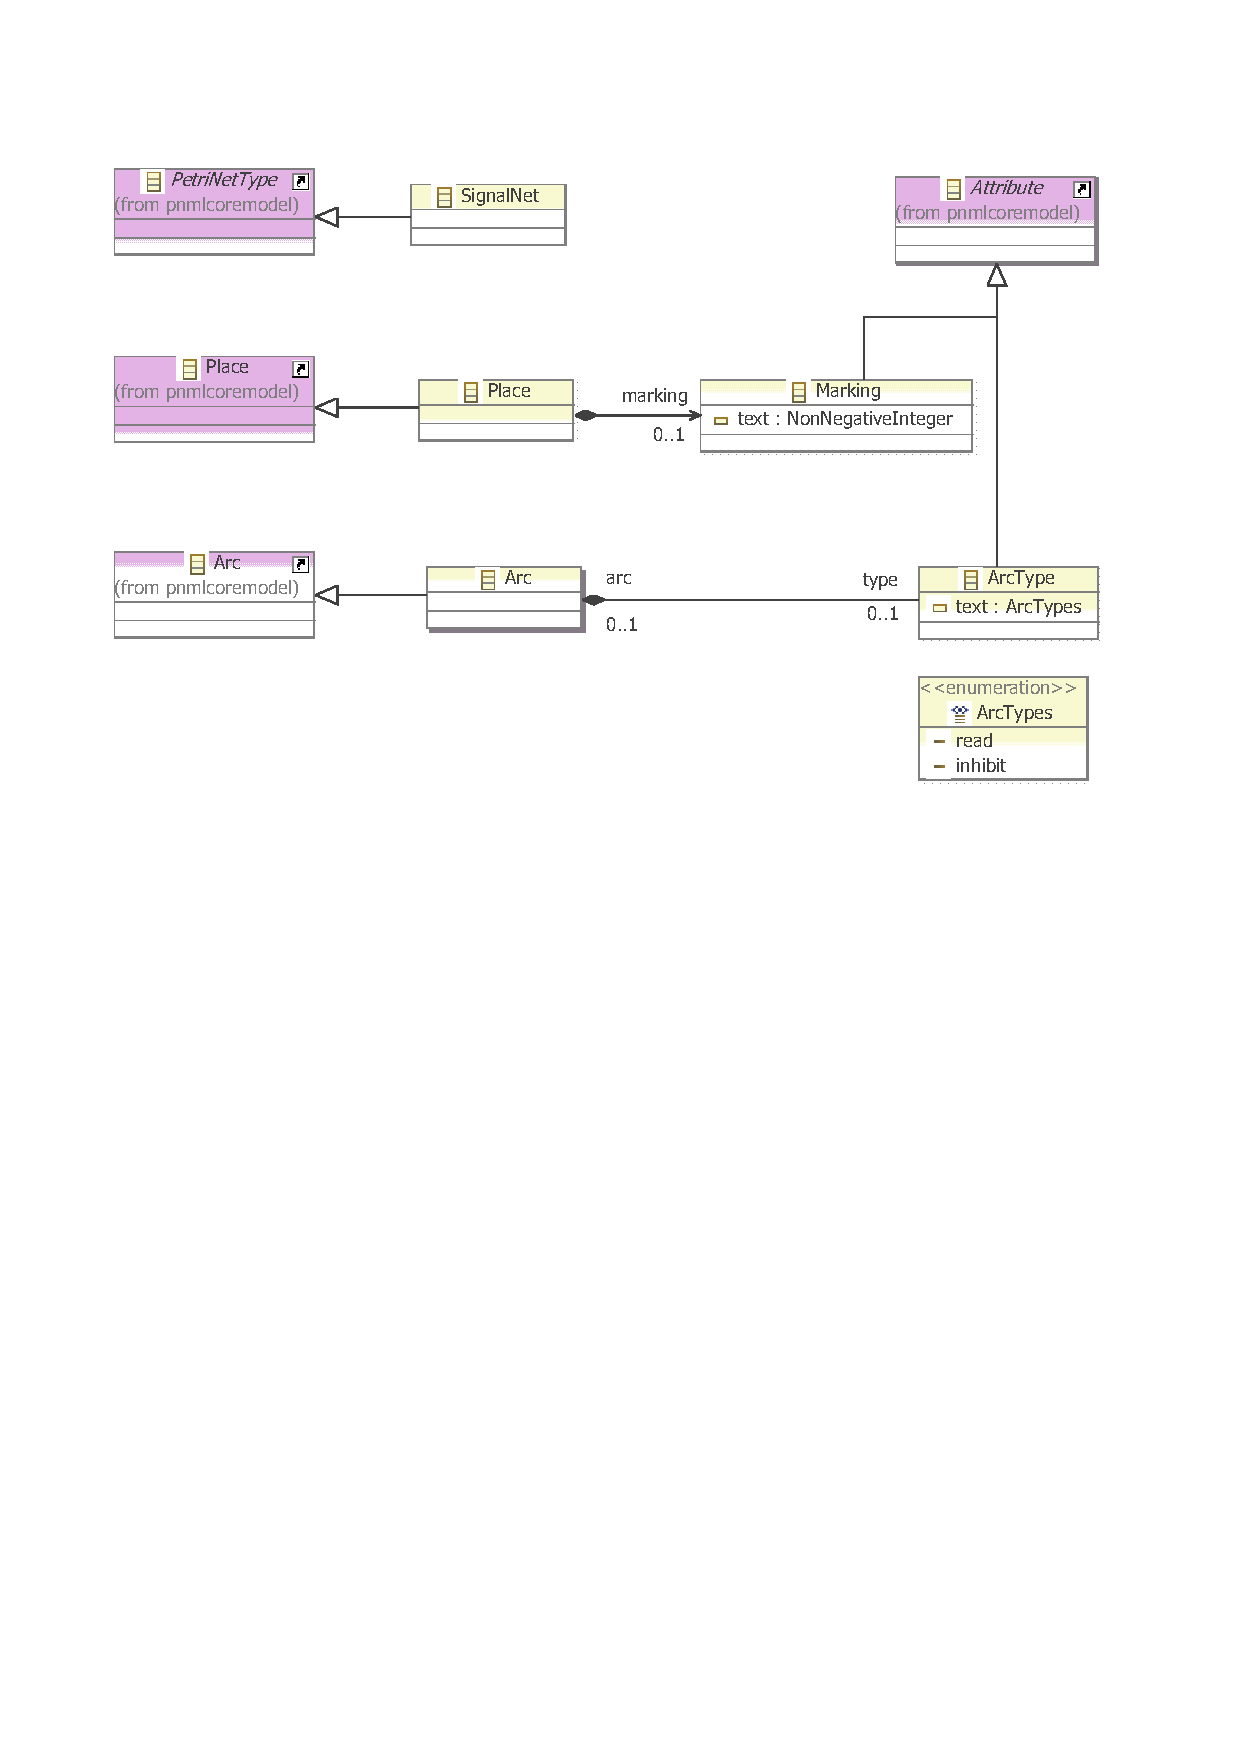
\includegraphics[scale=.60]{SE-Nets-PNTD}}
  \caption{The Ecore model for SE-Nets}
  \label{fig:SE-Nets-PNTD}
\end{figure}
%
Moreover, the Ecore model defines that there can be a {\tt Marking} for
places. Both label classes inherit from {\tt Attribute},%
  \index{ePNK!Attribute@{\tt Attribute}|DEF}
which means that these labels are not shown as annotations, but in the
properties view, when the respective arc or place are selected in the editor (see
Fig.~\ref{fig:signal-net-attributes}). We will see
Sect.~\ref{sec:dev:graphical}, how the value of these attributes can
be shown in the graphical representation
of the place or the arc. All we need to do for a label in the Petri net
type definition to be considered an attribute by the ePNK is deriving it
from the class {\tt Attribute} of the PNML core model.

If we have a closer look at the Ecore model from Fig.~\ref{fig:SE-Nets-PNTD},
we see that the class {\tt ArcType} has a reference {\tt arc} which points
back to the arc that ``owns'' that type -- the reference {\tt arc} is, actually,
an opposite of reference {\tt type}. This additional reference allows us to
navigate back from the arc type to the respective arc, which makes it easier
to formulate some constraints for arcs and their arc types\footnote
  {In the current version, this feature is not used, though.}%
. As we had discussed earlier in Sect.~\ref{subsubsec:PNTD-model}, classes
derived from {\tt Label} and also from {\tt Attribute} are not allowed to
have any feature other than the {\tt text} attribute. The reason for this
restriction is that PNML does not allow us to serialize this feature.
So, we need to make sure that such references to arcs are not serialized --
conceptually this is not necessary anyway, since the reference {\tt arc} is the opposite
of the reference {\tt type}. Therefore, we switch the serialisation
of the feature {\tt arc} off. This can done by selecting the resp.\ reference
in the editor for the Ecore model, and then, in the properties view, 
selecting the ``Advanced''\footnote
  {This ``Advanced'' section shows all kinds of advanced setting of the
   respective Ecore element. In case you are new to Ecore and you do not
   understand the concept of ``transient'', do not worry. Just ignore this for
   now.}
section, and then set the property ``transient'' to ``true'', meaning that this
feature is not serialised to a file (the ePNK serialisation mechanism takes that
into account).%
  \index{ePNK!Attribute|)}

From the Ecore model above, we can create the ``genmodel'' and generated the
model code and the edit code as discussed in Sect.~\ref{subsubsec:type-codegeneration}.
And we would need to do the same manual change: implement the {\tt toString()} method,
so that it returns the unique URI for that type; and we would need to make the
constructor of the class {\tt SignalNetImpl} public. In this example, however, we chose a
different way -- we create a class {\tt SignalNetFactory} that inherits from
{\tt SignalNetImpl} without any additional attributes, methods or constructors.
Since the implicit default constructor of {\tt SignalNetFactory} is public,
this will do the job. This is actually the preferred method, since regeneration
of the model code after a model change does not need any manual changes anymore.

Plugging in the Petri net type to the ePNK extension point works as described
in Sect.~\ref{subsubsec:simplePNTDplugin}. Listing~\ref{lst:SENetPlugin} shows
the resulting fragment of the ``plugin.xml'' (with some minor omissions).
%
\begin{figure}[htbp!]
\lstinputlisting[label=lst:SENetPlugin,language=XML,tabsize=2,stringstyle=\small,%
caption={Plugging in SE-Nets}]%
  {code/senet.xml}
\end{figure}

Listing~\ref{lst:SENetConstraint} shows the constraint for SE-nets, which makes
sure that an arc type can only be present for arcs that run from a place to a
transition; it also guarantees that arcs run from a place to a transition, from
a transition to a place, or between two transitions. It is a live constraint,
which needs to be checked, whenever the source or target of an arc are set,
and whenever the arc type is set.
%
\begin{figure}[htbp!]
\lstinputlisting[label=lst:SENetConstraint,language=XML,tabsize=2,stringstyle=\small,%
caption={Adding the constraint for SE-nets}]%
  {code/senet-constraint.xml}
\end{figure}

With these definitions, the ePNK would know what SE-nets are -- still the
inhibitor arcs and the signal arcs would not yet appear as shown in
Fig.~\ref{fig:signal-net-attributes}. To this end, we still need to
extend the graphical appearance of SE-nets, which will be discussed 
in Sect.~\ref{sec:dev:graphical}.%
  \index{SE-Nets|)}


\subsection{Petri net type definitions in general: HLPNG}
\label{subsec:complexPNTD}

In this section, we discuss some more advanced mechanisms that can be used for
defining new Petri net types. These mechanism will be discussed by the help
of the Petri net type definition of high-level Petri nets (HLPNGs). Therefore,
we start with an overview of the concepts of HLPNGs, from the implementation
point of view (for the conceptual part we refer to
Sect.~\ref{subsec:introHLPNG} and for a detailed discussion of all models and
concepts, we refer to \cite{HKea09}).

\subsubsection{Overview of HLPNGs}

As discussed in Sect.~\ref{subsec:introHLPNG}, HLPNGs have different kinds of
complex labels: \emph{declarations} of variables, sorts, and
operators; \emph{types} defining the sort of the tokens of a place,
\emph{markings} which are multiset terms defining the initial marking of a
place, \emph{conditions} as transition guards, and
\emph{arc annotations} that define which tokens are consumed, resp.\ produced
when a transition fires. What is more, the labels cannot be considered isolated from
each other anymore -- some labels, like markings, arc annotations, or
conditions may use \emph{symbols}%
  \index{ePNK!Symbol|DEF}
that are defined in other labels -- in particular, in the declarations.

Figure~\ref{fig:HLPNG-PNTD} shows the Ecore model defining the concepts of
HLPNGs, which can be found in the folder ``model'' in project\footnote
  {This is the plug-in in which HLPNGs are plugged into the ePNK; since HLPNGs
   are quite complex, and require many models, and also the implementation of
   a parser, the underlying concepts are defined in different other projects;
   all of these projects have a name with prefix {\tt
   org.pnml.tools.epnk.pntypes.hlpngs} -- some of them are generated
   automatically from models or from a grammar. You can import all
   of these projects to your workspace by the Eclipse ``Import As'' feature
   in the ``Plug-ins'' view.}
{\tt
org\qnsep{}pnml\qnsep{}tools\qnsep{}epnk\qnsep{}pntypes\qnsep{}hlpngs\qnsep{}pntd}.
This model follows the same principles as the model for PTNets, which was
discussed in Sect.~\ref{subsubsec:PNTD-model}.
%
\begin{figure} [btp!!] % [hbt!!]
  \centerline{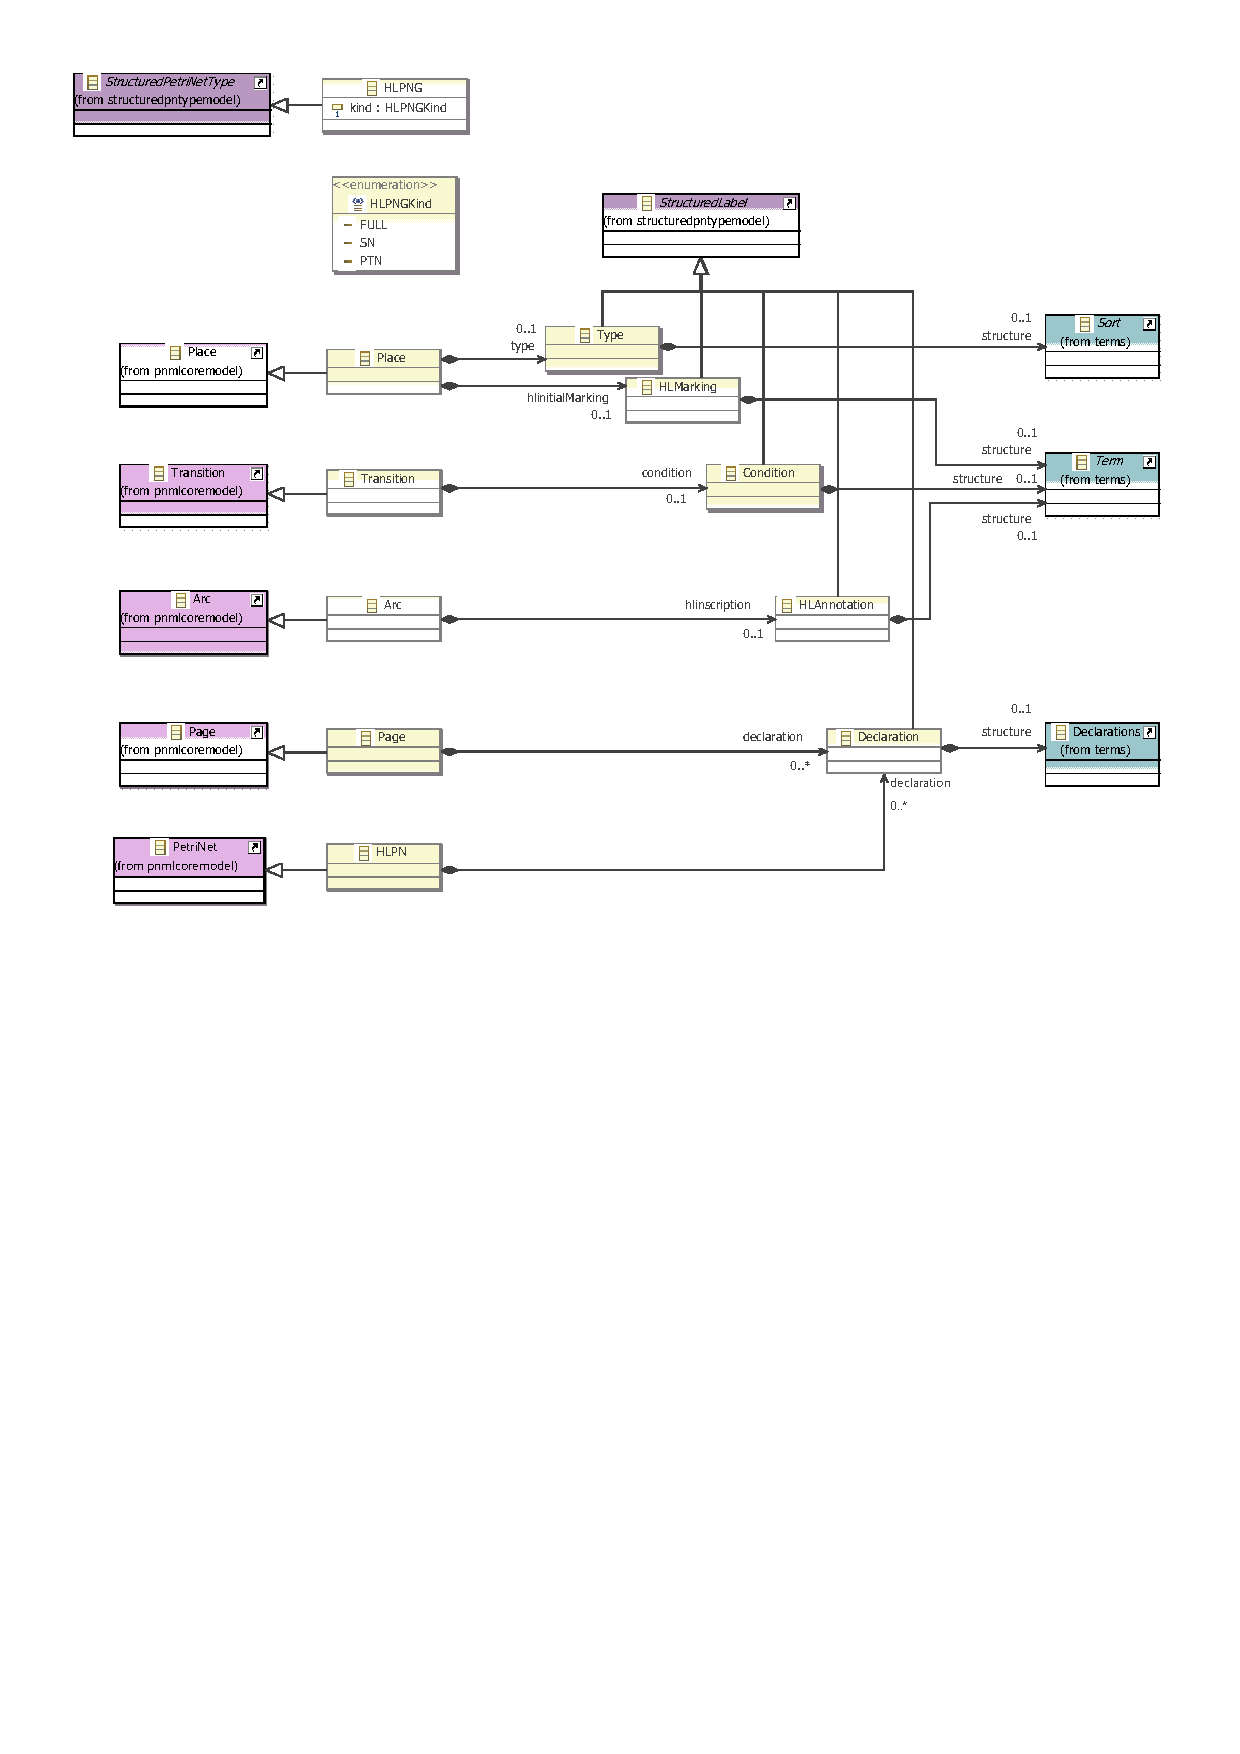
\includegraphics[scale=.67]{HLPNG}}
  \caption{The Ecore model for HLPNGs}
  \label{fig:HLPNG-PNTD}
\end{figure}
%
The main differences are that the defined Petri net type {\tt HLPNG} extends a
more advanced class {\tt StructuredPetriNetType}, and all labels extend
{\tt StructuredLabel}, which are part of the PNML core model. These two classes
provide the infrastructure needed for parsing the textual labels and for
establishing the links between these labels. This structure is discussed
in Sect.~\ref{subsubsec:structuredPNTs}.  

The actual contents of all these labels is defined in their containment {\tt
structure}; note that we use {\tt Term} as the contents for the labels {\tt
HLMarking}, {\tt Condition}, and {\tt HLAnnotation}, since all of them are terms -- just
with different additional constraints imposed on them (see
Sect.~\ref{subsubsec:PNTDConstraints}).
Note that by contrast to normal labels and attributes, \emph{structured labels}
can have -- actually must have -- a composition, which normally\footnote
  {The name could be changed, but this would require some programming, which
   will be discussed later.}
has the name {\tt structure}. But there should not be any other features than
that.

The detailed structure and concepts of terms, sorts, and declarations, are
defined in several other models. Since these details are not too relevant
for understanding the definition of structured Petri net types, we discuss
only the main part of that model.
%
\begin{figure}[btp!!] % [hbt!!]
  \centerline{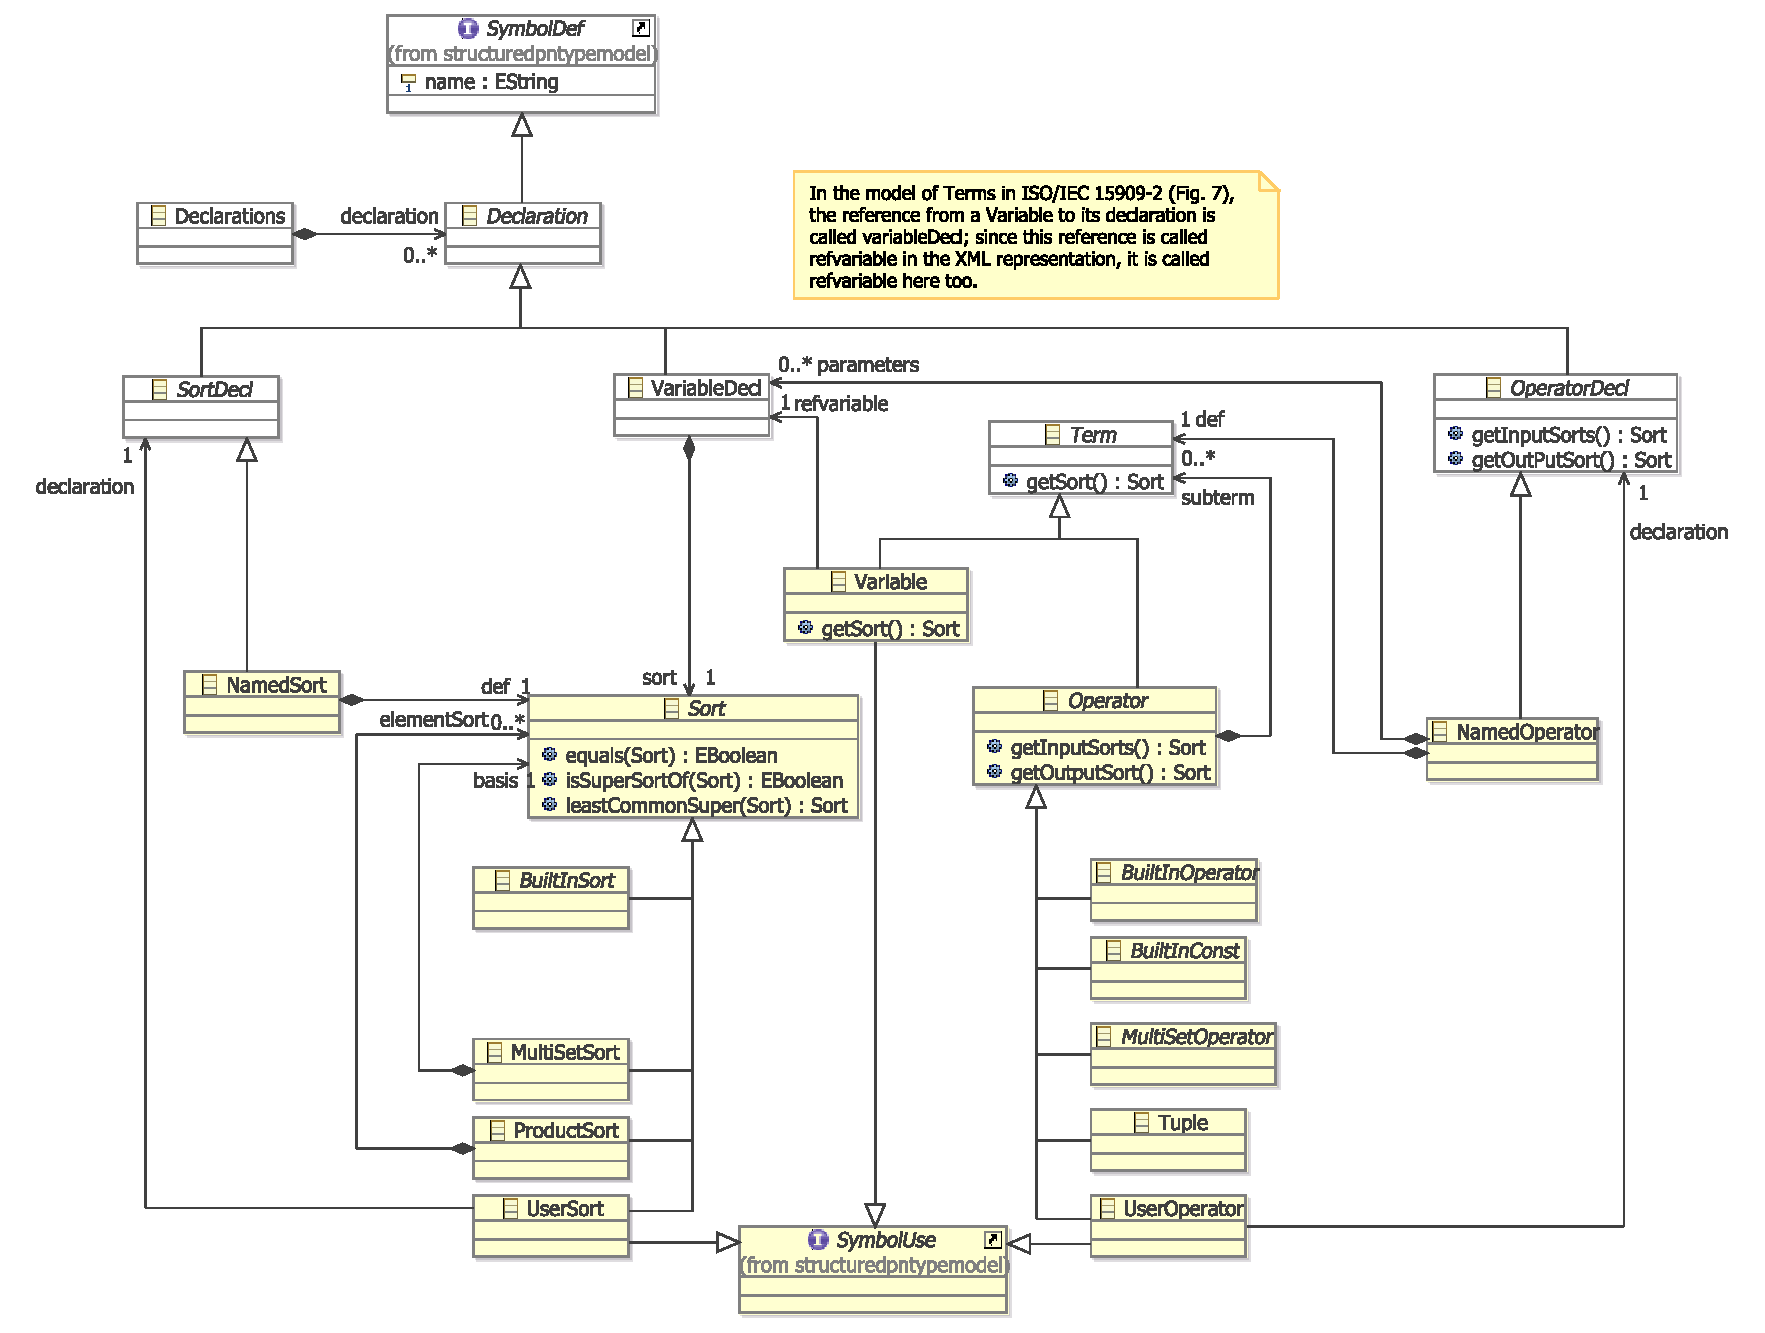
\includegraphics[scale=.45]{HLPNGDataTypes-Terms}}
  \caption{The Ecore model for the main concepts of HLPNGs}
  \label{fig:HLPNG-Terms}
\end{figure}
%
This part of the model is shown in Fig.~\ref{fig:HLPNG-Terms} -- this as well as
the diagrams of all the other models can be found in the plug-in {\tt
org.pnml.tools.epnk.pntypes.hlpngs.datatypes}. For a detailed discussion of
these models and their concepts, we refer to \cite{HKea09}. There is only one
important difference, which are the classes {\tt SymbolDef}%
  \index{ePNK!SymbolDef@{\tt SymbolDef}|DEF}
and {\tt SymbolUse},%
  \index{ePNK!SymbolUse@{\tt SymbolUse}|DEF}
which do not occur in the models of ISO/IEC~15909-2. 
These two classes are the ePNKs infrastructure for dealing with the definition
of symbols and their use in a uniform and generic way -- on the side, making the
concepts of \emph{symbol definition}%
  \index{ePNK!Symbol definition|DEF}
and \emph{symbol use}%
  \index{ePNK!Symbol use|DEF}
explicit, so that the model is more concise. These concepts are part of
the PNML core model concerning structured Petri net types, which will be
discussed in the next section.

\index{Net label|(DEF}%
One other issue worth noting in the Ecore model of Fig.~\ref{fig:HLPNG-PNTD} is
the class {\tt HLPN}, which extends class {\tt PetriNet}%
  \index{ePNK!PetriNet@{\tt PetriNet}|DEF}
from the PNML core model. This represents the Petri net itself. Normally, Ecore
models defining a new Petri net type would not need to extend the class
{\tt PetriNet} itself; it would be enough to extend the class {\tt
PetriNetType}.%
  \index{ePNK!PetriNetType@{\tt PetriNetType}|DEF}
HLPNGs, however, have so-called \emph{net labels},
which are labels that are directly attached
to the net -- and not to a page. For net types with net labels, the class
{\tt PetriNet} must be extended and equipped with compositions to the respective
labels -- in our example, these are declarations. But, we would
discourage defining such net labels for Petri nets types.%
\index{Net label|)}

\subsubsection{Structured Petri net types and structured labels}
\label{subsubsec:structuredPNTs}
\index{ePNK!structured Petri net type|(DEF}
\index{ePNK!structured label|(DEF}

As mentioned above, the ePNK provides some general interfaces and infrastructure
for defining structured Petri net types, which distill the general concepts of
more complex Petri net types. This is, again, captured in models (and the
code generated from them).

The model for structured Petri net types can be found in the ``model''
folder of the ePNK core project {\tt org\qnsep{}pnml\qnsep{}tools\qnsep{}epnk}:
{\tt PNMLStructured\optsep{}PNTypeModel}.
The diagram is shown in Fig.~\ref{fig:PNMLStructuredType}.
%
\begin{figure}[hbt!!]
  \centerline{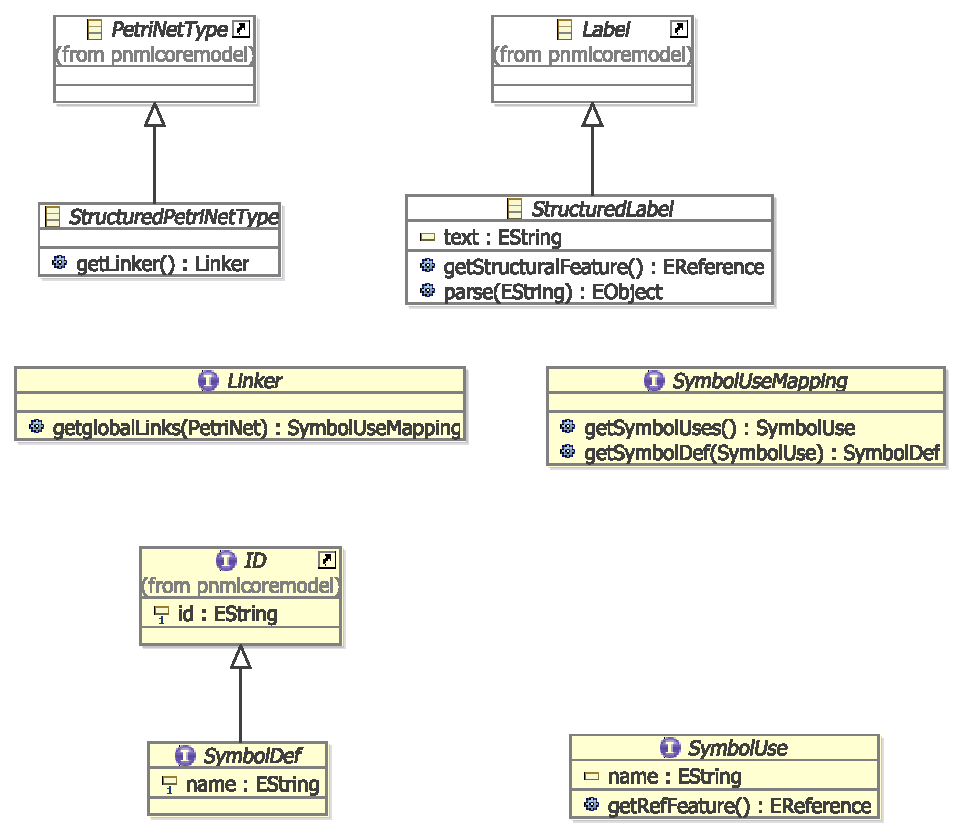
\includegraphics[scale=.60]{PNMLStructuredPNTypeModel}}
  \caption{The model for structured Petri net types}
  \label{fig:PNMLStructuredType}
\end{figure}
%
We know the classes {\tt PetriNetType} and {\tt Label} as well as the
interface {\tt ID}, which is used for all ePNK elements that have an id,
already from the PNML core model. The abstract class {\tt StructuredLabel}%
  \index{ePNK!StructuredLabel@{\tt StructuredLabel}|DEF}
extends the class {\tt Label}, it has an attribute {\tt text}, which stores
the contents of this label as a text String. The actual structural contents
is defined by classes that extend it (we have seen
some examples in Fig.~\ref{fig:HLPNG-PNTD} already). Since, the ePNK cannot
not know these concrete implementations, classes extending the structural
label must make the reference to this structural contents known to the
ePNK. This is achieved by the method {\tt getStructuralFeature()};%
  \index{ePNK!getStructuralFeature@{\tt getStructuralFeature()}|DEF}
as long as the feature for the structure is called `structure' in the model, we
do not need to do anything in the implementation (the ePNK will access this
feature in a reflective way); only if for some reason, the model chooses a
different name, this method must be implemented manually. Moreover, every class
for a structural label must provide a method {\tt parse()}%
  \index{ePNK!parse@{\tt parse()}|DEF}
for parsing a String
-- a representation of this label in concrete syntax; an implementation of this
method may return null, if the text cannot be parsed. If the label could be
parsed,  it must return some object (to be precise an {\tt EObject} which is the
EMF version of objects) with all the substructure of that label -- the abstract
syntax of the label. In particular, that object must have a type that is
compatible with the label's structural feature. This method must be implemented
manually for every new extension since the ePNK cannot guess the concrete syntax.

The abstract class {\tt StructuredPetriNetType}%
  \index{ePNK!StructuredPetriNetType@{\tt StructuredPetriNetType}|DEF}
has one additional method, which must provide a {\tt Linker}%
  \index{ePNK!Linker@{\tt Linker}|DEF} 
for linking the uses of some symbols to their definitions, which are captured by
classes {\tt SymbolDef}%
  \index{ePNK!SymbolDef@{\tt SymbolDef}|DEF}
and {\tt SymbolUse}.%
  \index{ePNK!SymbolDUse@{\tt SymbolUse}|DEF} 
A {\tt SymbolDef} has an {\tt ID}%
  \index{ePNK!ID@{\tt ID}|DEF} 
and has a name, which will be used to refer to it (the id is internal to PNML
and the ePNK). This name will be used in {\tt SymbolUse}, again as
attribute name, to refer to the definition. The feature that actually refers to the definition, can
be accessed via the method {\tt getRefFeature()}.%
  \index{ePNK!getRefFeature@{\tt getRefFeature()}|DEF}
Since the ePNK does not know anything about how to make these connections, the
Petri net type needs to provide access to the linker; to this end, the class
{\tt StructuredPetriNetType} has a method {\tt getLinker()},%
  \index{ePNK!getLinker@{\tt getLinker()}|DEF}
which must be implemented by classes that extend it. {\tt Linker} is an
interface: a single method {\tt getglobalLinks()},%
  \index{ePNK!getglobalLinks@{\tt getglobalLinks()}|DEF}
which takes a Petri net and returns a {\tt SymbolUseMapping},%
  \index{ePNK!SymbolUseMapping@{\tt SymbolUseMapping}|DEF}
which is also an interface. Conceptually, the class {\tt SymbolUseMapping} maps
every {\tt SymbolUse} to its definition {\tt SymbolDef}. All the symbol uses for
which there exists a mapping, can be obtained (as a list) via the method
{\tt getSymbolUses()};%
  \index{ePNK!getSymbolUses@{\tt getSymbolUses()}|DEF}
and for each symbol use, the method
{\tt getSymbolDef()}%
  \index{ePNK!getSymbolDef@{\tt getSymbolDef()}|DEF}
will return the definition of that symbol. 

With this infrastructure, the ePNK can deal with all kinds of structured
labels. We will have a look at the implementation of some examples next:  We
consider the label {\tt Condition} in the Petri net type definition for HLPNGs
again (see Fig.~\ref{fig:HLPNG-PNTD}) -- the other labels are similar. Its
structural feature is the containment {\tt structure} to class {\tt Term}.
Since this is the standard name for structured labels, we do not need to
override the method {\tt getStructuralFeature}.%
  \index{ePNK!getStructuralFeature@{\tt getStructuralFeature}|DEF}
But, we need to implement the {\tt parse()} method.  The parsers for all labels
of HLPNGs were automatically generated by Xtext, and are made available in a
singleton class {\tt HLPNGParser} in package
{\tt org.pnml.tools.epnk.pntypes.hlpngs.datatypes.concretesyntax}
in a project with the same name. For parsing a term, class {\tt HLPNGParser}
provides a method {\tt parseTerm(String)}. This singleton and its method
{\tt parseTerm()} is used in the implementation of {\tt ConditionImpl}
(you will find it in the package
{\tt org.pnml.tools.epnk.pntypes.hlpng.pntd.hlpngdefinition.impl}
in project {\tt org.pnml.tools.epnk.pntypes.hlpng.pntd}).

Since linking is across all the different labels of a net, there is only a
single linker for every net. For HLPNGs, this is implemented in the package
{\tt org\qnsep{}pnml\qnsep{}tools\qnsep{}epnk\qnsep{}pntypes\qnsep{}hlpngs\qnsep{}datatypes\qnsep{}concretesyntax\qnsep{}linking}
in project {\tt
org\qnsep{}pnml\qnsep{}tools\qnsep{}epnk\qnsep{}pntypes\qnsep{}hlpngs\qnsep{}datatypes\qnsep{}concretesyntax}.
This class is {\tt HLPNGLinker}; basically it goes through the complete Petri net twice; in the first round, it creates a symbol table of all symbol
definitions; in the second round, this symbol table is used to look up the
definition for every symbol use, which is stored in the {\tt SymbolMapping},
which implements the {\tt SymbolUseMapping} that we discussed above.

To make this linker known to the ePNK, the class {\tt HLPNGImpl} in
package {\tt
org.pnml.tools.epnk.pntypes.hlpng.pntd.hlpngdefinition.impl} implements the
method {\tt getLinker()}: it returns an instance of {\tt HLPNGLinker}.

Note that, in order to plug in the Petri net type definition to the ePNK,
we need to make the constructor public in the
class {\tt HLPNGImpl}, and we need to implement the {\tt toString()} method
so that it returns the unique URI of HLPNGs method
(as discussed in Sect.~\ref{subsubsec:simplePNTDplugin}).%
  \index{ePNK!structured Petri net type|)}%
  \index{ePNK!structured label|)}

\subsubsection{Constraints}
\label{subsubsec:PNTDConstraints}
\index{ePNK!Constraints|(DEF}
\index{ePNK!Java constraint|(DEF}

For HLPNGs, we needed to implement quite many constraints. As an example
for a \emph{Java constraint}, we discuss one of these constraints here. The rest
of them would not provide much insight into the mechanisms of the ePNK -- though they
might provide some insights to the inner workings of HLPNGs themselves.
There is also an OCL constraint that forbids connecting places with places
and transitions with transitions. But, this is exactly the same as for PTNets,
which is why we do not discuss it here again.

All constraints for HLPNGs are defined in the project
{\tt
org\qnsep{}pnml\qnsep{}tools\qnsep{}epnk\qnsep{}pntypes\qnsep{}hlpng\qnsep{}pntd},
the implementations of the Java constraints can be found in the package
{\tt org\qnsep{}pnml\qnsep{}tools\qnsep{}epnk\qnsep{}pntypes\qnsep{}hlpng\qnsep{}pntd\qnsep{}validation}
We discuss the constraint that transition conditions must have type boolean,
which is implemented in class {\tt ConditionIsBoolType}.
Listing~\ref{lst:constraintCondIsBool} shows this class.
%
\begin{figure}[htbp!]
\lstinputlisting[label=lst:constraintCondIsBool,tabsize=2,stringstyle=\small,%
caption={The constraint that conditions have type boolean}]%
{code/ConditionIsBoolType.java}
\end{figure}
%
This constraint extends the class {\tt AbstractModel\optsep{}Constraint}%
  \index{EMF!AbstractModelConstraint@{\tt AbstractModelConstraint}|DEF}
from EMF Validation and implements the method {\tt validate()}.%
  \index{EMF!validate@{\tt validate()}|DEF}
From the validation context, it obtains the target object, which should be a
transition (see later). But, we are defensive and check that explicitly. Then, we
obtain the condition label of that transition, and if it is not {\tt null},
get the term (its structure). Then, we check whether the sort of
the term is boolean\footnote
 {The implementation of {\tt getSort()} for terms is actually quite
  complex; it amounts to implementing a type system for the
  annotation language of HLPNGs. But we do not discuss the details here.}%
. If it is not, we return a failure status via the validation context,
and add the transition and the textual label to an array of objects
(which is used in the error message to be defined later). Otherwise,
we return a success status. Note that the EMF Validation Framework
makes sure that this validate method is called for all transitions
of a selected Petri net, Petri net document or page, once it is
properly plugged in, which is discuss below.

Plugging in a Java constraint is similar to plugging in
OCL constraints. The relevant fragment of the ``plugin.xml''
is shown in Listing~\ref{lst:HLPNGJavaConstraint}.
%
\begin{figure}[htbp!]
\lstinputlisting[label=lst:HLPNGJavaConstraint,language=XML,tabsize=2,stringstyle=\small,%
caption={Adding the constraint for conditions}]%
  {code/hlpng-constraint.xml}
\end{figure}
%
The main differences are that the attribute {\tt lang} is ``Java''
now and the attribute {\tt class} refers to the class {\tt ConditionIsBoolType},
which was discussed above. As target class, the transition class of
HLPNGs is defined (that is why we could assume that the target
object is a transition). Another difference is that this is no live constraint,
but a batch constrain. This means, that the constraint might be violated during
editing; a violation will be detected and reported only when the user
explicitly invokes the validation.
Since this is a batch constraint, we do not need to declare any events in
the target.

Another difference to the OCL constraint is, that we can refer to several
parameters in the message now. What the different parameters are, depends
on the return value of the validation method. In our case, this was
the transition (or its String representation) and the text of the label.

The ellipses (``...'') indicate that the constraint that we have discussed
here, is just one of many other constraint, which are not discussed here.%
  \index{ePNK!Constraints|)}
  \index{ePNK!Java constraint|)}

\subsubsection{XML Mappings}
\label{subsubsec:XMLmapping}
\index{ePNK!XML mapping|(DEF}

In the sections above, we have discussed how to define a Petri net type and
all its concepts and constraints. For saving it in PNML, it is also necessary
to define how these concepts are represented in XML -- at least if the
``standard mappings'' do not work.

In this section, we discuss how these mappings are defined. Conceptually,
these mappings are tables (in ISO/IEC~15909-2, these tables are given
in Clause~7.3.1). In the ePNK, these tables are ``programmed'' as part
of the new Petri net type\footnote
  {It might be, that a future version of the ePNK will provide a means to plug
  in these tables directly in some form; but since ``programming the tables'' is
   not too difficult, this does not have a high priority.}%
.  

We explain the concepts of these ``programmed tables'' by discussing some
of the mappings for HLPNGs. The tables for a new Petri net type are
programmed, by overwriting the method
{\tt registerExtended\optsep{}PNMLMetaData(\optsep{}ExtendedPNMLMetaData
metadata)} of {\tt PetriNetType}; the parameter {\tt meta\optsep{}data}
represents the table, to which the entries should be added when the method is called.

Let us have a look at some examples. Listing~\ref{lst:xml-simple-mapping} shows
an excerpt of the {\tt registerExtendedPNMLMetaData()}%
  \index{ePNK!registerExtendedPNMLMetaData@{\tt
  registerExtended PNMLMetaData()}|DEF} method of the class {\tt HLPNGImpl},
  which implements the Petri net type for HLPNGs.
%
\begin{figure}[htbp!]
\lstinputlisting[label=lst:xml-simple-mapping,tabsize=2,stringstyle=\small,%
caption={Mappings for type, marking, and condition extensions}]%
{code/xml-mapping-simple.java}
\end{figure}
%
Each of the {\tt metadata.add} statements defines one table entry, which
defines the mapping of one specific feature of the Ecore model to an
XML element (we will see later how to map an Ecore attribute to an XML
attribute). The three statements shown in Listing~\ref{lst:xml-simple-mapping}
define how the structure feature of the labels {\tt Type}, the {\tt HLMarking},
and the {\tt Condition} are mapped to the XML element {\tt \verb+<structure>+}.
We discuss the first one, the {\tt Type}, in more detail:
\begin{itemize}
  \item The first parameter, denotes the feature that is mapped to XML by this
        entry; in this case, it is the composition from the class {\tt Type} to
        the class {\tt Sort} (see Fig.~\ref{fig:HLPNG-PNTD} on
        page~\pageref{fig:HLPNG-PNTD}). The source and target classes are
        mentioned explicitly as second and third parameter again. We refer to
        the feature and the two classes via the singleton classes that describes
        the elements of the packages (HLPNGdefinition and Terms), which
        are automatically generated by EMF. These
        \emph{package classes},%
			\index{EMF!Package class}
        provide access to all the classes and features
        within a package (see \cite{BSM06} for more details). Note that {\tt
        HlpngdefinitionPackage.eINSTANCE} refers to the package {\tt
        hlpngdefinition} and {\tt TermsPackage.eINSTANCE} to the package {\tt
        terms}.
        
  \item As mentioned above, the second parameter denotes the class to
        which the feature belongs (it could be a sub-class of {\tt Type}
        in principle); this is often called the \emph{container class}.%
          \index{EMF!Container class|DEF}
        
  \item The third parameter denotes the class that the feature refers to
        (this could also be a sub class of {\tt Sort}); this is often called the
        \emph{object class}.%
          \index{EMF!Object class|DEF}
        
  \item The forth parameter defines the XML representation, the string
        that will be used as XML element in the serialisation of this
        feature (in our example ``structure'').
        
  \item The fifth parameter could refer to an XML attribute, that might
        be necessary for creating an Ecore object from the XML element
        (we will discuss an example later). In most cases, this XML attribute
        is not needed, since the XML element (and the context in which it
        occurs) provide enough information for creating the Ecore element from
        it.
        
  \item The last parameter refers to a factory that is capable of creating
        an Ecore instance of the respective class from the XML element
        and -- if provided -- the XML attribute. This parameter can
        be left empty, when the Ecore instance can be constructed reflectively
        from the information on the object class only.   
\end{itemize}

The ePNK uses this table and its entries in two directions: In the one
direction, the table is used to serialise a Petri net to its XML
syntax; in the other direction, the table is used to create the model
elements from the XML syntax.
In the latter case, the \emph{factories}%
  \index{ePNK!Factory|DEF}%
  \index{ePNK!IPNMLFactory@{\tt IPNMLFactory}|DEF}
play an important role. Listing~\ref{lst:factory-interface} shows the interface
that all these factories must implement.
%
\begin{figure}[htbp!]
\lstinputlisting[label=lst:factory-interface,tabsize=2,stringstyle=\small,%
caption={Interface {\tt Factory}}]%
{code/IPNMLFactory.java}
\end{figure}
%
The methods {\tt canCreateObject()}%
  \index{ePNK!canCreateObject@{\tt canCreateObject()}|DEF}
and {\tt createObject()}%
  \index{ePNK!createObject@{\tt createObject()}|DEF}
have the same parameters, which basically reflect the entries of the table that
we discussed above. Only the third (representing the object class) and the six one
(the factory itself) are missing. And, there is an additional parameter
({\tt provider}), which will provide access to the values of all attributes of
the currently read XML element (in case the factory needs the values of some
of the XML element's attributes for creating an object of the appropriate type).
The method {\tt canCreateObject()} is used to find out whether the factory is able
to create an object from the provided information, the {\tt createObject()}
method is used to actually create it. The {\tt createAttributeObject} is
used to create an object for some XML attribute. The implementation of these
factories is straightforward and a bit boring -- we do not discuss the
details here. You can have a look into the class {\tt HLPNGFactory}
in package {\tt
org\qnsep{}pnml\qnsep{}tools\qnsep{}epnk\qnsep{}pntypes\qnsep{}hlpng\qnsep{}pntd\qnsep{}hlpngserialisation\qnsep{}factory}
in the project {\tt org\qnsep{}pnml\qnsep{}tools\qnsep{}epnk\qnsep{}pntypes\qnsep{}hlpng\qnsep{}pntd} to get some
inspiration. What is more, with an extension that came into version 0.9.0
of the ePNK, the factory can be set to {\tt null}. In which case the
standard mechanism for creating an object of the target class will
be used; therefore, we need factories only in very special
cases. In most of the cases, the factory can be set to {\tt null}\footnote
  {Note that except for two features, which were used to test this
   new mechanism, the mappings for HLPNGs have not been updated 
   yet; therefore, you will find factories all over these mappings.
   But, this has historic reasons only and will eventually be
   changed (making the mappings more maintainable and easier to understand).}%
.

\begin{figure}[tbp!] % [htbp!]
\lstinputlisting[label=lst:xml-attribute-mapping,tabsize=2,stringstyle=\small,%
caption={Mappings of an attribute}]%
{code/xml-attribute-mapping.java}
\end{figure}
%
Listing~\ref{lst:xml-attribute-mapping} shows an example\footnote
  {Actually, this is the only example of this kind in HLPNGs.}
of how a feature of the model can be mapped to an XML attribute. In this
example, the value of the boolean constant is mapped to the XML attribute 
{\tt value}. This is where the method {\tt createAttributeObject()}%
  \index{ePNK!createAttributeObject@{\tt createAttributeObject()}|DEF}
of the factory comes into play.

The discussion above, gives a general idea of how these tables and mappings
work. All this, however, could have been achieved with the existing mechanisms
of EMF: Extended Metadata. Some of the PNML constructs cannot be
mapped to XML by the mechanisms provided by EMF Extended Metadata.
Therefore, the ePNK needed to provide its own mechanism for mapping
Ecore concepts to XML. In the rest of this section, we discuss some of
these special situations.

To this end, we consider the serialisation of the simple term {\tt
x`f(x,x)}, where {\tt x} is a variable and {\tt f} is a user defined operator.
The PNML representation is shown in Listing~\ref{lst:subterm-xml}, where ``5''
is the unique id of variable {\tt x} and ``1'' is the id of the user defined
operator {\tt f},
%
\begin{figure}[tbp!] % [htbp!]
\lstinputlisting[label=lst:subterm-xml,language=XML,tabsize=2,stringstyle=\small,%
caption={PNML representation of {\tt x`f(x,x)}}]%
{code/subterm.xml}
\end{figure}
%
In addition to being a bit verbose, there is one thing that is special about
this mapping: There is an XML element \verb+<subterm>+ for the association
form the top-level term (number of) to its subterm,
which are represented as two other XML elements,
\verb+<variable>+  and \verb+<useroperator>+. The XML element 
\verb+<subterm>+ defines to which feature of the term the XML element that is
contained in it should go. The XML element inside (e.\,g.\ 
\verb+<variable>+) defines the type that this object should have.

The problem here, is that there is an intermediate XML element that has no
object as counter part in the model -- it represents an association. We call
such an XML element an \emph{association element}.%
  \index{ePNK!Association element|DEF}
The mapping for these association elements is shown in
Listing~\ref{lst:xml-assoc-mapping}.
%
\begin{figure}[htbp!]
\lstinputlisting[label=lst:xml-assoc-mapping,tabsize=2,stringstyle=\small,%
caption={Mappings of associations to XML elements}]%
{code/xml-assoc-mapping.java}
\end{figure}
%
The first entry is actually as we have seen it before. The only difference
is that the factory produces an instance of a new class
{\tt TermAssoc}, which has the nature of a term but, actually, represents
an association to a term. We will discuss that class in more
detail later. The two other mappings, define the mapping of variables
and user operators to XML, and these are different, since they do not
refer to any feature at all. They just refer to a container class and 
a contained class. The container class is the class {\tt TermAssoc},
which will make sure that the variable resp.\ user operator will be added
to the subterm feature of the operator on the level above\footnote
  {There would actually be another way of doing this, in a slightly more
   elegant way when using ``standard features'', which
   will be discussed later in this section.}%
.

The class {\tt TermAssoc} does not need to be programmed. This class,
as well as the other classes for representing association elements, could
completely be generated from a model. This model is shown in Fig.~\ref{fig:AssocClasses}.
These classes extend a specific class of our model (the one to which the
respective association should go), and the general class for {\tt AssocClass},
which is defined by the ePNK, and implements all the necessary functionality.
%
\begin{figure}[btp!!]% [hbt!!]
  \centerline{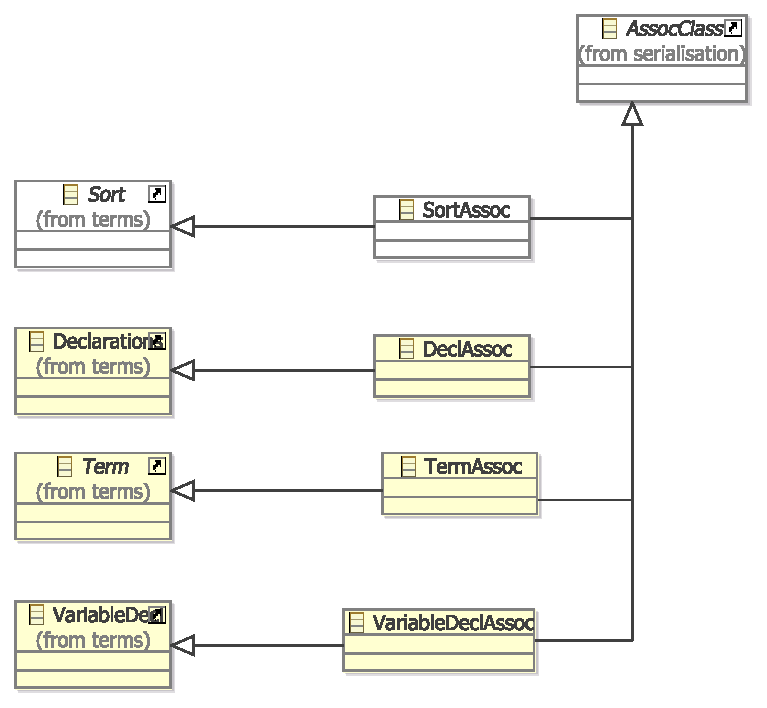
\includegraphics[scale=.60]{HLPNGSerialisation}}
  \caption{The package {\tt hlpngserialisation}}
  \label{fig:AssocClasses}
\end{figure}
%
Note that these classes will not occur in the model anymore, once it is
completely loaded -- they are only used while a PNML file is loaded.

In the case of subterms, every subterm occurs in a separate \verb+<subterm>+
element -- even if a term has several subterms, there is one subterm element
for each of them (see Listing~\ref{lst:subterm-xml}). In the case of parameters
of an operation declaration, this is different: Listing~\ref{lst:xml-parameters}
shows the PNML representation of the declaration of a named operator
{\tt f(x:INT, y:INT) =  x * y}.
%
\begin{figure}[htbp!]
\lstinputlisting[label=lst:xml-parameters,language=XML,tabsize=2,stringstyle=\small,%
caption={PNML structure for declaration {\tt f(x:INT, y:INT) =  x * y}}]%
{code/parameters.xml}
\end{figure}
%
Here, all variable declarations occur in the same \verb+<parameter>+ element.
We called these \emph{bundled association elements}.%
  \index{ePNK!bundled association element|DEF}
The table entries for this
mapping are shown in Listing~\ref{lst:xml-bundles}. The first one, is almost the
same as for association elements, and the Factory {\tt HLPNGFactory}
would create an instance of {\tt VariableDeclAssoc} for an XML element
\verb+<parameter>+. The new last parameter {\tt true} says, that this is
a bundled association.
%
\begin{figure}[tbp!]
\lstinputlisting[label=lst:xml-bundles,tabsize=2,stringstyle=\small,%
caption={Mapping bundled association elements}]%
{code/xml-bundles.java}
\end{figure}
%
The second table entry defines the mappings for variable entries, which
is independent of the context, which is why the first to parameters are
{\tt null}. We call this a \emph{context independent element mapping}.%
  \index{ePNK!context independent element|DEF}
  
This context independent element mapping can be applied in any other
context. In combination with another special case of mappings which we
call \emph{standard feature},%
  \index{ePNK!standard feature|DEF}
this is a very powerful mechanism. For example, for {\tt Declarations} and
sub-elements for which context independent element mappings exist (in the
example, there would be variable declarations, sort declarations, and
operator declarations), all these elements should be added to this standard
feature. The table entry shown in Listing~\ref{lst:xml-standard-feature} defines
the composition {\tt declaration} as the standard feature of {\tt Declarations}.
%
\begin{figure}[htbp!]
\lstinputlisting[label=lst:xml-standard-feature,tabsize=2,stringstyle=\small,%
caption={Defining a standard feature}]%
{code/xml-standard-feature.java}
\end{figure}
%
Note that there is no mapping to XML here. A standard feature of an element just
says that, whenever there comes some context independent element that is not
mapped explicitly to a feature, this element should be added to the standard
feature of the model. Of course, there should only be one standard feature --
otherwise there would be some ambiguities.%
  \index{ePNK!XML mapping|)}

\subsection{Petri net type definitions: Summary and overview}
\label{subsec:pntd:summary}

In Sect.~\ref{subsec:simplePNTD}--\ref{subsec:complexPNTD}, we have seen most
of the mechanisms for defining new Petri net types. Basically, a Petri net
type definition  consists of a new Ecore package where the Petri net
type of the PNML core model is extended and the classes for the extended Petri
net elements are modelled. Form this model the major parts of the code
(model and edit code) can be generated. In the generated code, some
manual changes need to be made. The Ecore package needs to follow some
modelling principles that are discussed in Sect.~\ref{subsubsec:PNTD-model} and
the manual changes are discussed in Sect.~\ref{subsubsec:type-codegeneration}.
All the extensions must be added as \emph{labels} of the respective kind
of node of the Petri net.

If a label should not be shown as annotation of the respective element
in the graphical editor of the ePNK, this can be achieved by deriving it from
the ePNK class {\tt Attribute}. Attributes can be edited in the properties view
of the ePNK only. Sect.~\ref{subsec:PNTD:SE-Nets} discussed an example.

More complex Petri net types might require to also implement a parser
and to store the actual information of the label not only as text but also
as an abstract syntax tree in the PNML file. Such labels are called
structured labels and have been discussed in
Sect.~\ref{subsubsec:structuredPNTs}. In case of complex Petri net types,
it might also be necessary to customize the XML representation, of the
labels and the concepts of its abstract syntax. To this end, the ePNK
allows Petri net types to define a XML mapping, which is discussed in
Sect.~\ref{subsubsec:XMLmapping}.

For all kinds of nets, it is possible to add additional constraints
on top of the Ecore model of the respective type. These constraints are
plugged in via the standard mechanisms for EMF Validation. Two examples
are discussed in Sect.~\ref{subsubsec:simplePNTDconstraints} and
Sect.~\ref{subsubsec:PNTDConstraints}. The constrains can either be
programmed in Java or can be OCL.

Note that it is possible to extend the class {\tt PetriNet} of
the PNML core model (when net labels are needed in the Petri net type).
It is also possible to add labels to pages and reference nodes by
extending the respective classes in the Ecore model for the new
Petri net type.

When an annotation is defined for a page, the question is whether the
respective annotation should be shown as a label annotated to the
node page on the super page or whether the label should be shown
as a page label on the page itself. The name of a page is
  \index{ePNK!Page label|DEF}
shown as an annotation of the page on the super page; by default, an
annotation of a page is shown as page labels on the page itself,
if there can be multiple annotations of that kind for the page;
and it is shown as a label of the page node on the super page,
if there can be only one annotation of that kind. But, this can
be changed by overriding the method {\tt showLabelOnPage()}%
  \index{ePNK!showLabelOnPage@{\tt showLabelOnPage()}|DEF}
of the class {\tt Page} of the respective Petri net type -- which requires
manual coding again.%
  \index{ePNK!Petri net type definition|)} 


\section{Defining the graphical appearance}
\label{sec:dev:graphical}

For some kinds or Petri nets, some places, transitions or arcs should be
shown in a dedicated graphical representation. And the graphical appearance
might depend on the context of the respective element -- and the graphical
appearance might change dependent on the changes of the context of this element.
An example are signal arcs, inhibitor arcs, and read arcs in SE-nets, an
example of which is shown in Fig.~\ref{fig:dev:signal-net-graphics} again.

\begin{figure}[hbt!!]
  \centerline{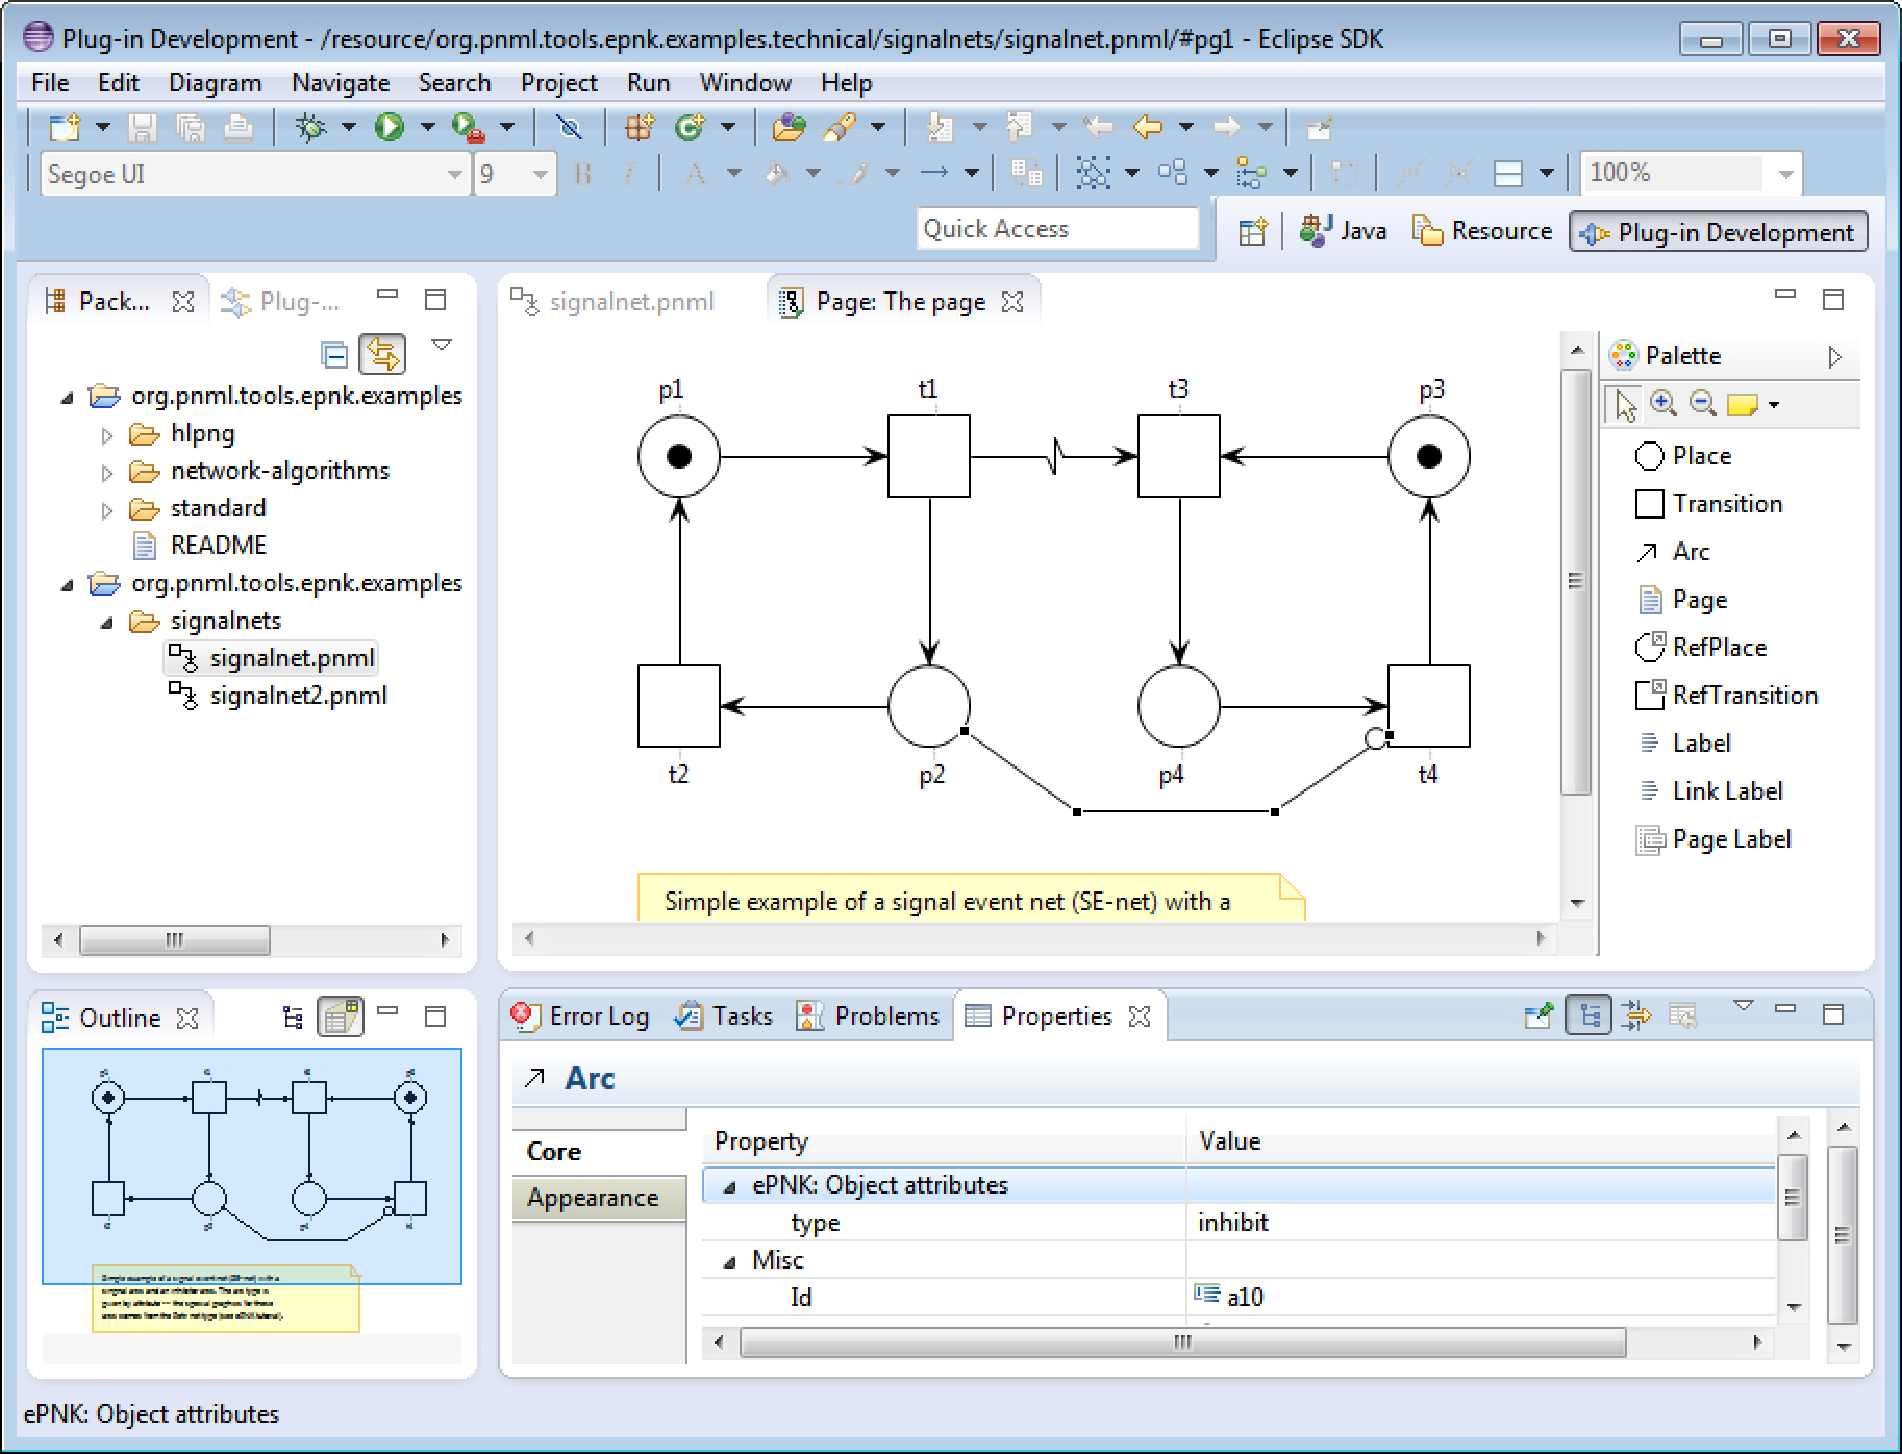
\includegraphics[scale=.38]{signalnet-attributes}}
  \caption{A SE-net with its dedicated graphics}
  \label{fig:dev:signal-net-graphics}
\end{figure}

In this section, we discuss how such dedicated graphics can be plugged
into the ePNK. To this end, we continue the discussion of the projects that
implement SE-nets, which was started in Sect.~\ref{subsec:PNTD:SE-Nets}. 
As you can see from Fig.~\ref{fig:dev:signal-net-graphics}, SE-nets have a
dedicated graphics for arcs (as signal arc, read arc, or inhibitor arc).
But there is also a dedicated graphics for places: the marking is shown
by black dots -- up to some upper bound -- in the respective places.

We start discussing the implementation of the dedicated graphical representation
for arcs. To this end, we need to implement a \emph{figure class},%
  \index{GMF!Figure class|DEF}
which is the GEF/GMF terminology for the graphically visible elements (view) of
a model element in an editor. Listing~\ref{lst:graph-ext-se-net1} shows the main
part of the class {\tt SignalnetArcFigure}, which implements the graphical appearance
of the arcs of SE-nets (the class {\tt SignalnetArcFigure} can be found in the
package {\tt org.pnml.tools.epnk.pntypes.signalnets.graphics.figures} of
plug-in project {\tt org.pnml.tools.epnk.pntypes.signalnets}).
%
\begin{figure}[htbp!]
\lstinputlisting[label=lst:graph-ext-se-net1,tabsize=2,stringstyle=\small,%
caption={The class {\tt SignalnetArcFigure}: main part}]%
{code/SignalnetArcFigure1.java}
\end{figure}
%
This class extends the class {\tt ArcFigure} of the ePNK. In line~3, an
enumeration of possible arc types is define, which is private to this class. Note that we do
not re-use the enumeration from the model here, but define another enumeration,
in order to make the implementation a bit simpler. The current type of the arc
is stored as an attribute of this class (line~5). The constructor (lines
7--11) takes the arc (the model element behind this figure) as a parameter;
it calls the constructor of the super class {\tt ArcFigure}%
  \index{ePNK!ArcFigure@{\tt ArcFigure}|DEF}
of the ePNK, which also takes the arc as a parameter, then calculates the
current type (by the private method {\tt getType()}, which is shown in
List.~\ref{lst:graph-ext-se-net2}) and then properly sets
the graphical features by calling the method {\tt setGraphics()}, which is specific to this class.

The method {\tt setGraphic()} changes the graphical features of the arc
according to the current type of the arc (lines 21--39). In this example,
we change the \emph{decorations}%
  \index{GMF!Decoration|DEF}
of the arc only; we use the decorations at both ends (source and target). As
decorations, we use the usual arrow shaped ones ({\tt
ReisigArrowHeadDecoration}\footnote {This name was chosen in honour of Wolfgang Reisig, who insisted on
   arrow heads in Petri nets being drawn in a very specific way. The
   implementation of {\tt ReisigArrowHeadDecoration} tries to meat
   Wolfgang Reisig's standards.}%
), circles ({\tt CircleDecoration}), and flashes ({\tt FlashDecoration}),
which are provided by the ePNK.%
  \index{ePNK!Arc decoration|DEF}
In the method, the variables for the decorations on both ends are initialized
to {\tt null} (lines 22-23). Then, dependent on the type of the arc the
respective decorations are set. Note that the {\tt FlashDecoration} is attached to
the source, but it will actually show up in the middle of the arc (or
actually in the middle of the first segment of the arc)  by the specific way it
is is implemented. The reason for this choice is that there can be at most
one decoration at each end of a \emph{connection}.%
  \index{GMF!Connection|DEF}
Since signal arcs have two decorations, the flash and the arrow head, one needs
to be at the source end of the connection. In the end, the only thing
that is necessary to do is actually setting the decorations -- note that calling
the respective methods with {\tt null}, means that there is no decoration for
that connection.

Note that changes in the underlying model might make changes in the
graphical appearance necessary. Such a change could be an explicit change of
the type of the arc by the end user or just reconnecting an arc to
a different kind of element. Whenever such a change happens, the ePNK
notifies the figure of the affected model element by calling
the method {\tt update()},%
  \index{ePNK!update@{\tt update()}|DEF}
which is specific to all extensible figure classes of the ePNK. It should be
overridden by the extending classes. Lines 14--19 of
List.~\ref{lst:graph-ext-se-net2} show the implementation of this method in our
example. The type of the arc is computed again; if it changed, the {\tt
setGraphics()} method is called again.

This is all there is to do for implementing another appearance of an
arc. Of course, this figure still needs to be plugged in, which is
discussed later. In the update method, you could do all kinds
of other changes such as changing the colour of the arc ({\tt
setForeGroundColor()}%
  \index{GMF!setForeGroundColor@{\tt setForeGroundColor()}|DEF}
or the line style ({\tt setLineStyle()})%
  \index{GMF!setLineStyle@{\tt setLineStyle()}|DEF}
 -- and many things more.

If you need other decorations than the ones that come with the ePNK, you can
implement them yourself. But, we do not discuss this here since this is
a GMF or, actually, an Eclipse draw2d concept. A look at the implementation of
the ePNK decorations might give you a clue.

Listing~\ref{lst:graph-ext-se-net1} shows the last part of the class {\tt
SignalnetArcFigure}: the implementation of method {\tt  getType()}. This
is mostly straightforward: computing the type based on the information
of the arc underlying this figure. The only surprise might be the
initial type check of {\tt this.arc} for {\tt Arc}. The reason is
that {\tt this.arc} refers to a final attribute of {\tt ArcFigure}
of the ePNK, which refers to the {\tt Arc} of the PNML core model,
whereas in the class {\tt SignalnetArcFigure}, we need to refer to the {\tt
Arc} of the SE-net package -- which has the same name, but in a different
package.
%
\begin{figure}[htbp!]
\lstinputlisting[label=lst:graph-ext-se-net2,tabsize=2,stringstyle=\small,%
caption={The class {\tt SignalnetArcFigure}: compute type}]%
{code/SignalnetArcFigure2.java}
\end{figure}

In the above example, we have changed the appearance of the arc on a
very high level of programming, by changing the attributes of the figure.
And if the desired graphical appearance can be achieved this way, this
is the recommended way of doing this. In some cases, however, changing
the attributes of the figure it not enough -- we rather would need to
``draw'' some additional things. This can be done by using a different
strategy for extending the figure: overriding the {\tt fillShape()}%
  \index{GMF!fillShape@{\tt fillShape()}|DEF}
or {\tt outlineShape()}
  \index{GMF!outlineShape@{\tt outlineShape()}|DEF}
methods. We explain this strategy by another example:
showing the initial marking by a respective number of black tokens in the place.
Listing~\ref{lst:graph-ext-se-place} shows the class {\tt SignalnetPlaceFigure},
which implements this graphical appearance.
%
\begin{figure}[htbp!]
\lstinputlisting[label=lst:graph-ext-se-place,tabsize=2,stringstyle=\small,%
caption={The class {\tt SignalnetPlaceFigure}}]%
{code/SignalnetPlaceFigure.java}
\end{figure}
%
The {\tt update()}%
  \index{ePNK!update@{\tt update()}|DEF}
method just informs the figure that it should repaint itself\footnote
  {We could have done that in a slightly smarter way so that
   repaint is called only if the marking has changed -- as for the arcs.}
when something has changed. The actual appearance is now defined by
overriding the method {\tt fillShape()}. In this method, first, all
the normal drawing of the place is done by calling the same method of the
{\tt super} class. After that, the marking of the place is computed\footnote
  {Since this requires some navigation in the model, this is delegated
   to a separate method {\tt getMarking()}, which is not discussed here.}%
. If the marking is between 1 and 4, the respective number of tokens
are drawn in the client area of the place. To this end, the drawing
methods on the {\tt graphics} object are used. Depending on the number of
tokens, the appropriate positions are chosen (note that for space
reasons, we omit the code for drawing four tokens). If there are more than four
tokens, they are not represented as black circles anymore. They are ``drawn'' as
a string representing the number of tokens.

Note that you could do more things and could also use some other low-level
methods of figures to do that. But, we do not discuss that here. You
might get some more inspiration my looking at another tutorial which
implements some more exotic appearances of arcs, places and transitions
in project {\tt org.pnml.tools.epnk.extensions.tutorial.types}; the
resp.\ figures can be found in the in package
{\tt org\qnsep{}pnml\qnsep{}tools\qnsep{}epnk\qnsep{}extensions\qnsep{}%
tutorial\qnsep{}types\qnsep{}arctypes\qnsep{}graphicalextensions\qnsep{}figures}.

At last we need to make the new figures defined for SE-nets known to
the ePNK -- we need to plug them in. This is done by implementing and
plugging in  a factory for these figures.
%
\begin{figure}[htbp!]
\lstinputlisting[label=lst:graph-ext-se-factory,tabsize=2,stringstyle=\small,%
caption={The factory class {\tt SignalnetGraphics}}]%
{code/SignalnetGraphics.java}
\end{figure}
%
The factory for the graphical extension for SE-nets is shown in
List.~\ref{lst:graph-ext-se-factory}. It extends the abstract ePNK
class {\tt GraphicalExtension}.%
  \index{ePNK!GraphicalExtension@{\tt GraphicalExtension}|DEF}
The first method (line 4--8) defines, for which types of Petri nets this
extension provides some graphics -- as a list of classes of the respective Petri
net types. In our example, this is the class representing SE-nets -- obtained
from the automatically generated package class. The second method (line 11--18)
defines for which kinds of elements there is a specific graphics -- again
represented as a list of class objects. In our example, these are the classes
representing the arc and the place of SE-nets. At last, there are two methods,
that create the respective figure object for an element by using the
respective constructors of the figure classes. Note that {\tt
GraphicalExtension} has also methods for creating a figure for
transitions and other kinds of nodes -- but we do not need to override them
here since our extension does not provide special graphics for them.

Actually the class {\tt GraphicalExtension} has some more methods, 
which define priorities for the graphical extensions -- in case more
than one graphical extension is plugged in and applies to the same
element. And it can also be defined, whether a graphical extension should apply
to all subtypes of a Petri net type or not.  The meaning of the methods
is documented as Java doc comments for the methods in the interface for
the factory {\tt IGraphicalExtension}.%
  \index{ePNK!IGraphicalExtension@{\tt IGraphicalExtension}|DEF}  

At last, the graphical extension needs to be plugged in to the
ePNK.  The relevant part of the ``plugin.xml'' of the project is shown
in List.~\ref{lst:graph-ext-se-plugin}. This is straightforward. The
attribute ``point'' of the extension refers to the ePNK extension
point {\tt org.pnml.tools.epnk.diagram.graphics}, and the class
attribute of the graphicsextension refers to the factory of
List.~\ref{lst:graph-ext-se-factory}.  
%
\begin{figure}[htbp!]
\lstinputlisting[label=lst:graph-ext-se-plugin,language=XML,tabsize=2,stringstyle=\small,%
caption={Plugging in the graphical extension}]%
{code/graphical-extension-se-net-plugin.xml}
\end{figure}

With this extension installed, the SE-nets should now look like the one
in Fig.~\ref{fig:dev:signal-net-graphics}.

\section{Adding tool specific information}  
\label{sec:adding-toolspecific-info}
\index{ePNK!Tool specific information|(DEF}  

As discussed in Sect.~\ref{subsec:PNMLcoremodel}, the PNML allows tool specific
information to be added to all elements of Petri nets -- indicated by the
special XML element \verb+<toolspecific>+. The ePNK reads and writes any tool
specific information, and, in principle, the contents of these tool
specific extensions could be accessed and modified via the class {\tt AnyType},
which is defined in the plug-in {\tt org.eclipse.emf.ecore}. But this
is tedious and, basically, means navigating in the element's XML structure.

Therefore, the ePNK provides an extension point for plugging in tool specific
extensions, so that they can be accessed and modified via an API specific to the
extension which can be defined in terms of a model. We will discuss how to
use this extension point by the help of an example: the token positions, which
is a tool specific extension mandated by ISO/IEC~15909-2:2011. We have seen an
example already in Fig.~\ref{fig:sample-net} and Listing~\ref{lst:sample-net} on
page~\pageref{lst:sample-net}.

This tool specific extension is defined in the project
{\tt org\qnsep{}pnml\qnsep{}tools\qnsep{}epnk\qnsep{}toolspecific\qnsep{}tokenpositions}.
Most of this code in this project as well as the ``plugin.xml'' was
automatically generated by EMF from the Ecore model ``Tokenpositions.ecore''
in the folder ``model''. This model is shown in Fig.~\ref
{fig:ToolSpecificTokenPosModel}.
%
\begin{figure}[hbt!!]
  \centerline{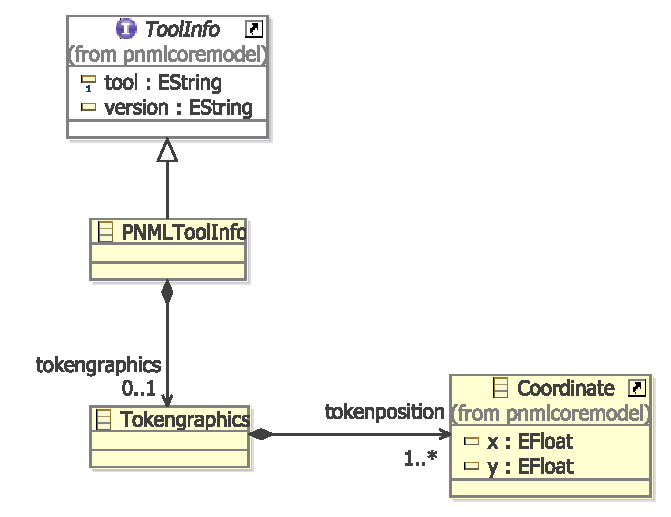
\includegraphics[scale=.60]{Tokenpositions}}
  \caption{The model for tool specific extension tokenpositions}
  \label{fig:ToolSpecificTokenPosModel}
\end{figure}
%
The new classes are {\tt PNMLToolInfo} and {\tt Tokengraphics}. The class 
{\tt PNMLToolInfo} represents the actual tool specific information: it must
implement the PNML core model interface {\tt ToolInfo}.%
  \index{ePNK!ToolInfo@{\tt ToolInfo}|DEF}
The actual contents of this tool specific information is {\tt Tokengraphics},
which consists of one or many coordinates; the class {\tt Coordinate} is
re-used from the PNML core model. 

From this model, the code can be generated in the same way as described in
Sect.~\ref{subsubsec:type-codegeneration}. First, the ``genmodel'' must be
created, and from the ``genmodel'', the model code and the edit code must be
generated.

After the code generation, the only thing left to do is to manually create a
factory for this tool specific extension, and use this factory for plugging
it into the ePNK. The factory for our extension is shown in
Listing~\ref{lst:tool-spec-extension-factory}.
%
\begin{figure}[htbp!]
\lstinputlisting[label=lst:tool-spec-extension-factory,tabsize=2,stringstyle=\small,%
caption={Factory for the tool specific extension}]%
{code/TokenpositionsExtensionFactory.java}
\end{figure}
%
The factory implements the ePNK interface {\tt ToolspecificExtensionFactory},%
  \index{ePNK!ToolspecificExtensionFactory@{\tt ToolspecificExtension
    Factory}|DEF}
which consists of four methods. The two methods {\tt createToolInfo()}%
  \index{ePNK!createToolInfo@{\tt createToolInfo()}|DEF}
create an instance of this tool specific extension; the method with the two
String parameters, {\tt tool} and {\tt version} is used, when the tool
name and version are given, which might return instances of different classes --
in our example, however, the version number is irrelevant. The two other
methods, must return the tool name for that extension and its version, which, in
our example, are encoded as constants.

Listing~\ref{lst:tokenpositions-plugin} shows the fragment of the ``plugin.xml''
that is needed to plug in the token position extensions to the ePNK. In
addition to the name and the id, there is an attribute {\tt class}
that defines the factory for the tool specific extension; this class must
implement the interface {\tt Toolspecific\optsep{}ExtensionFactory}.
%
\begin{figure}[htbp!]
\lstinputlisting[label=lst:tokenpositions-plugin,language=XML,tabsize=2,stringstyle=\small,%
 caption={Plugging in the token position extension}]%
{code/tokenpositions-plugin.xml}
\end{figure}
%
Moreover, there is a brief description of this extension. 

Note that the ePNK does not provide any way yet of explicitly defining the XML
syntax of these extensions. The standard XMI serialisation will be used --
which is compliant with ISO/IEC~15909-2:2011 for tool specific extensions.
Eventually, the ePNK might provide a mapping mechanism similar to the one
for Petri net types.%
  \index{ePNK!Tool specific information|)}

\section{Overview of the ePNK and its projects}
\label{sec:overviewAPI}

In this section, we give a brief overview of the different parts of the ePNK,
the project structure and where to look for different kinds of functionality in
the ePNK API an its projects. As mentioned earlier, developers should not change
anything in these projects. Anyway, this overview should help to better understand the ideas
behind the ePNK, the necessary dependencies (that need to be included in
new projects via the  ``plugin.xml'') and the functions that are available in
the ePNK API, which could be used by developers in their extensions. Note that
we do not discuss the details of the API here. In particular, we do
not discuss the API concerning the code that is generated from the Ecore
models (model and edit code) since it is mostly straightforward.
Section~\ref{subsubsec:ePNK:API:EMF} gives a brief overview of the main
principles behind the model code that is generated from Ecore models; for
more information, we refer to the EMF book \cite{BSM06}.

Like all extensions of Eclipse, the ePNK is organized in many Eclipse projects,
which together make the ePNK. Most of these projects are so-called plug-in
projects; and these are the ones most relevant for developers, since
these are the projects to look up the API and to which extensions need to
refer (in form of dependencies). In addition, there are some projects, which
contain documentation only (like this manual), there are some projects that
do not contain any code, but from which other projects are generated; and
there are so-called features, which define collections of plug-in projects in
order to deploy them. And there is a project for generating the ePNK update site
from the features.

In this manual, we focus on the plug-in projects of the ePNK, the most important
of which are listed below. We start with an overview of the ePNK core projects,
which make up the framework of the ePNK\footnote
  {Technically, all these plug-in projects are part of the ePNK features
   {\tt org.pnml.tools. epnk.core}  and
   {\tt org.pnml.tools.epnk.extensions.basic}.}%
:
\begin{description}
  \item[{\tt org.pnml.tools.epnk}:] ~\\
  This is the core project of the ePNK. In
  this project, you will find the PNML core model, some additional models, and the
    \emph{model code}, that was generated from them. All the models, can be
    found in the folder ``model''. The PNML core model is contained in
    {\tt PNMLCoreModel\qnsep{}ecore};%
        \index{PNML Core Model|DEF}
    in order to avoid clutter in the graphical
    diagram, the core model is actually split up into three separate diagrams:
    {\tt PNMLCore\optsep{}Model\qnsep{}ecorediag} contains the most important
    concepts; {\tt PNMLCore\optsep{}Model\optsep{}Graphics\qnsep{}ecorediag}
    contains the graphical features of PNML; and {\tt PNMLCoreModelProxies\qnsep{}ecorediag} contains some extensions
    to the PNML core model that are necessary to maintain labels in the
    graphical editor of the ePNK by so-called \emph{label proxies}%
      \index{ePNK!Label proxy|DEF}
    and \emph{page label proxies}.%
      \index{ePNK!Page label proxy|DEF}
   These proxy elements, however, are not of any concern for normal developers.

    There are four other models in this project: {\tt PNMLDataTypes.ecore}
    defines the \emph{data types}%
       \index{ePNK!Data types|DEF}
    for non-negative and positive numbers, which are used instead of the
    respective XML Schema Data Types of ISO/IEC 15909-2. {\tt
    PNMLStructuredPNTypeModel\qnsep{}ecore} defines the concepts of structured
    Petri net types%
      \index{ePNK!structured Petri net type|DEF}
    (see Sect.~\ref{subsubsec:structuredPNTs}).
    {\tt Serialisation\qnsep{}ecore} provides some general structure that is
    used for the XML serialisation of so-called association elements%
      \index{ePNK!Association element|DEF}
    (see Sect.~\ref{subsubsec:XMLmapping}).
    {\tt PNMLPageDiagram\optsep{}Info\qnsep{}ecore} is the model for storing the
    GMF diagram information%
      \index{ePNK!Diagram information|DEF}
    for pages as ePNK tool specific information in PNML models, which are not of
    concern for normal developers.
    
    This project provides also some \emph{convenience classes}%
      \index{ePNK!Convenience classes|DEF}
    in package {\tt org\qnsep{}pmm\qnsep{}tools\qnsep{}epnk\qnsep{}helpers},
    which might be helpful in practice. The class {\tt FlatAccess}%
      \index{ePNK!FlatAccess@{\tt FlatAccess}|DEF}
    allows handling a Petri net that is
    distributed over several pages as if it was flat (see
    Sect.~\ref{subsec:tutorial-MC} for an example).
    Another convenience class is {\tt NetFunctions},%
      \index{ePNK!NetFunctions@{\tt NetFunctions}|DEF}
    which provides many static methods for finding out to which net an element
    belongs, what the type of this net is, and for obtaining lists of
    elements of some kind of a given Petri net.
    
    In this plug-in, also the two extension points of the ePNK are defined:
    one for defining new Petri net types (PNTD), another for defining 
    new tool specific extensions.%
      \index{ePNK!PNTD}%
      \index{ePNK!Tool specific extension}
    
    In addition to the model code, also the so-called edit code and editor
    code are generated from these models, which together define the tree
    editor for PNML (see below).
    
    Note that, in this project, also the constraint context and the
    constraint category {\tt org\qnsep{}pnml\qnsep{}tools\qnsep{}epnk\qnsep{}validation},%
      \index{ePNK!Validation}%
      \index{ePNK!Constraints|DEF}
    to which all other constraints for new Petri net types should be added, are
    defined here (see Sect.~\ref{subsubsec:simplePNTDconstraints}
    and~\ref{subsubsec:PNTDConstraints}).
    
  \item[{\tt org.pnml.tools.epnk.edit}:] ~\\
    This project contains the edit code
    that was generated from the models in project {\tt org.pnml.tools.epnk}.
    Though most of this code was automatically generated from the models,
    there are several manual changes, that enable generically dealing with
    plugged in Petri net type definitions.
    
    Moreover, the generated standard EMF images in the folder {\tt icons}
    were replaced by nicer ones.
    
  \item[{\tt org.pnml.tools.epnk.editor}:] ~\\
    This project contains the editor
    code for the EMF tree editor for PNML that was generated from the models in
    project {\tt org\qnsep{}pnml\qnsep{}tools\qnsep{}epnk}. In this project,
    there are only a few, but crucial extensions, that made it possible to
    integrate the EMF tree editor with the graphical editor for pages (see the
    plug-in project
    {\tt org\qnsep{}pnml\qnsep{}tools\qnsep{}epnk\qnsep{}diagram} below).
              
  \item[{\tt org.pnml.tools.epnk.pntypes}:] ~\\
    This project contains the model
    and the generated model code for P/T-nets ({\tt PTNet}),%
        \index{ePNK!PTNet@{\tt PTNet}}
    as well as the extension that plugs in this type to the ePNK. The model code
    is completely generated from the model {\tt PTNet.ecore} in the folder
    ``model'', except for two changes in class {\tt PTNetImpl} as discussed in
    Sect.~\ref{subsec:simplePNTD}.

  \item[{\tt org.pnml.tools.epnk.pntypes.edit}:] ~\\
    This is the project with the
    edit code that was generated from the Ecore model {\tt PTnet\qnsep{}ecore}
    of project {\tt org\qnsep{}pnml\qnsep{}tools\qnsep{}epnk\qnsep{}pntypes}.
    There are no manual changes in the generated code -- only the icons in the
    folder {\tt icons} were replaced by nicer ones.
    
  \item[{\tt org.pnml.tools.epnk.toolspecific.tokenpositions}:] ~\\
    In this project,
    the tool specific extension for token positions%
        \index{Token positions|DEF}
    (as defined in ISO/IEC~15909-2) is defined (see
    Sect.~\ref{sec:adding-toolspecific-info}). The model code and the edit
    project {\tt org.pnml.tools.epnk.toolspecific.token\-po\-si\-tions.edit}
    was generated (which does not contain any manual changes -- not even nicer icons) from the model
    {\tt Tokenposition.ecore}.

    Note that the ePNK does not take the information of these token positions
    into account in the graphical representation of places. The only reason they
    are defined in the ePNK is that ISO/IEC~15909-2:2011 mandates them
    -- and we use this extension as an example to show how to define tool specific
    extensions in Sect.~\ref{sec:adding-toolspecific-info}.
    
  \item[{\tt org.pnml.tools.epnk.actions}:] ~\\
    This project defines the
    standard actions of the ePNK, which are the pop-up menus for adding
    missing ids and for linking the labels of structured Petri net types
    (see Sect.~\ref{subsubsec:structuredPNTs}).
    
    Moreover, the classes {\tt AbstractEPNKAction}%
        \index{ePNK!AbstractEPNKAction@{\tt AbstractEPNKAction}|DEF}
    and {\tt AbstractEPNKJob}% 
         \index{ePNK!AbstractEPNKJob@{\tt AbstractEPNKJob}|DEF}
    are defined in this project, which are convenience classes to make it easier
    to define functions for the ePNK that run in the background (see
    Sect.~\ref{subsec:tutorial-MC}).
    
  \item[{\tt org.pnml.tools.epnk.diagram}:] ~\\
    This project contains the code for
    the GMF-generated graphical editor for pages of Petri nets. This code was
    generated from the GMF models in project {\tt org.pnml.tools.epnk.gmf}.
    But, there are major manual changes for making this graphical editor
    generic and for integrating it with the tree editor for PNML (see
    project {\tt org\qnsep{}pnml\qnsep{}tools\qnsep{}epnk\qnsep{}editor}).
    
    The package {\tt org.pnml.tools.epnk.gmf.extensions.graphics} and its%
      \index{ePNK!Customizing graphics|DEF}
    sub-packages {\tt decorations}%
      \index{ePNK!Decorations|DEF}
    and {\tt figures}%
      \index{ePNK!Figures|DEF}
    are relevant for 
    developers, who want to contribute specific graphical appearances for
    some Petri nets. Here you find the factory and the figures of the ePNK,
    which need to be extended for customizing the graphical appearance;
    and you can use the predefined ePNK decorations for that purpose
    (see Sect.~\ref{sec:dev:graphical} for more details). 
    
  \item[{\tt org.pnml.tools.epnk.gmf.integration}:] ~\\
    This project defines the
    pop-up menus for starting the graphical editor on a page that is selected in
    a tree editor or in a graphical editor.
    
  \item[{\tt org.pnml.tools.epnk.annotations}:] ~\\
    This project defines the
    infrastructure for annotating Petri nets by applications. Up to now,
    the annotations%
        \index{ePNK!Annotation|DEF}
    provide the most basic concepts only -- they will be extended in the
    future.

    A simple example of annotating the context of transitions was discussed
    in Sect.~\ref{subsec:developer:applications}.
    
  \item[{\tt org.pnml.tools.epnk.applications}:] ~\\
    This project provides the
    interfaces and classes for implementing and starting applications on Petri
    nets, which was briefly discussed in
    Sect.~\ref{subsec:developer:applications}.%
       \index{ePNK!Application|DEF}
    
  \item[{\tt org.pnml.tools.epnk.applications.view}:] ~\\
    This project implements
    the applications view, that shows all currently running implementations.
    Developers would typically not directly use this project. 
\end{description}

Next, we discuss some of the net types, and functions and applications, which we
had discussed in this manual as a tutorial\footnote
  {Technically, these plug-in projects come from the ePNK feature
   {\tt org.pnml.tools. epnk.extensions.tutorial}.}%
:
\begin{description}
  \item[{\tt org.pnml.tools.epnk.functions.tutorials}:] ~\\
    This project contains the functions that were discussed in
    Sect.~\ref{subsec:file-overview} and Sect.~\ref{subsect:multi-agent},
    which can serve as a guideline for defining own extension projects.
    
  \item[{\tt org.pnml.tools.epnk.functions.modelchecking}:] ~\\
     This project
     contains the model checker extension%
          \index{Model checker}
     for the ePNK that is discussed in Sect.~\ref{subsec:tutorial-MC}. Note that
     the project {\tt MCiE} is used in this model checker extension only (MCiE
     is not relevant for anything else in the ePNK -- except if you want to
     implement your own model checker based on MCiE).

 \item[{\tt
 org\qnsep{}pnml\qnsep{}tools\qnsep{}epnk\qnsep{}tutorials\qnsep{}applications}:]  ~\\
    This project implements an example of an application%
      \index{ePNK!Application}
    using annotations.%
        \index{ePNK!Annotation|DEF}
    It contains the code for the transition context application which was
    discussed in Sect.~\ref{subsec:developer:applications}.
    
 \item[{\tt org.pnml.tools.epnk.pntypes.signalnets}:] ~\\
    This project is 
    the plug-in project implementing the Petri net type definition for SE-nets%
      \index{SE-nets|DEF}
    (see Sect.~\ref{subsec:PNTD:SE-Nets} and the graphical extensions for
    SE-nets (see Sect.~\ref{sec:dev:graphical}).

\item[{\tt org.pnml.tools.epnk.pntypes.signalnets.edit}:] ~\\
    This plug-in project
    contains the edit code, which is generated from the model of SE-nets
    -- without any manual changes      
\end{description}

The plug-in projects with the prefix {\tt org\qnsep{}pnml\qnsep{}tools\qnsep{}epnk\qnsep{}pntypes\qnsep{}hlpng}
resp.\ {\tt org\qnsep{}pnml\qnsep{}tools\qnsep{}epnk\qnsep{}pntypes\qnsep{}hlpngs} together are used for defining
high-level Petri nets (HLPNGs).%
  \index{ePNK!HLPNG|(DEF}
The following list gives an overview in a bottom
up way -- ending with the actual Petri net type definition for HLPNGs:

\begin{description}
\item[{\tt org.pnml.tools.epnk.pntypes.hlpngs.datatypes}:] ~\\
   In this project, all
   the models that define the concepts of sorts, operators, variables and terms
   for HLPNGs are contained. In particular, there is a model  {\tt
   HLPNGDataTypes.ecore} for the general structure of terms, declarations
   and the built-in sorts and operators that occur in all versions of HLPNGs.
   And there are many more models and diagrams for specific versions of
   HLPNGs (Clauses~5.3.2--5.3.12 of ISO/IEC~15909-2:2011).
 
\item[{\tt org.pnml.tools.epnk.pntypes.hlpngs.datatypes.concretesyntax}:] ~\\
   This project is an Xtext project that defines the grammar for the concrete
   syntax of the different labels of HLPNGs, from which a parser is generated.
   Here, we do not discuss the details of generating the parser. The manually written
   class {\tt HLPNGParser} accesses the automatically generated parsing
   operations and provides methods for parsing every
   kind of label of HLPNGs. The other important manually written class is
   {\tt HLPNGLinker}, which provides the global Linker for labels (as discussed
   in Sect.~\ref{subsubsec:structuredPNTs}).

   Note that the plug-in project ending with 
   {\tt concretesyntax\qnsep{}ui} was
   automatically created when the Xtext project was created by a wizard;
   it provides a stand-alone textual editor for the labels of HLPNGs.
   Since this stand-alone editor is not needed for the ePNK, this project is
   not part of the standard deployment of the ePNK. 

\item[{\tt org.pnml.tools.epnk.pntypes.hlpng.pntd}:] ~\\
   This project actually
   combines all the parts discussed above into a Petri net type definition for
   HLPNGs. The main model is {\tt HLPNG\optsep{}Definition.ecore}, which was
   shown in Fig.~\ref{fig:HLPNG-Terms}. The other model {\tt
   HLPNGSerialisation.ecore} defines the auxiliary classes that temporarily
   store XML elements that represent associations and are used and referred to
   in the XML mappings (see Sect.~\ref{subsubsec:XMLmapping}) .
   
   The global linker {\tt HLPNGLinker} from the project 
   {\tt org\qnsep{}pnml\qnsep{}tools\qnsep{}epnk\qnsep{}pntypes\qnsep{}hlpngs\qnsep{}datatypes\qnsep{}concretesyntax}
   above is made available in the Petri net type by
   manually implementing the method {\tt getLinker()} in class {\tt HLPNGImpl}.
   The {\tt parse()} method for the different structured labels are also
   manually implemented -- they refer to the different {\tt parserXXX()} methods
   of class {\tt HLPNGParser}%
     \index{ePNK!HLPNG|)}
   from the project
   {\tt org\qnsep{}pnml\qnsep{}tools\qnsep{}epnk\qnsep{}pntypes\qnsep{}hlpngs\qnsep{}datatypes\qnsep{}concretesyntax}
   above.
   
\item[{\tt org.pnml.tools.epnk.helpers.unparse}:] ~\\
   This project implements
   a serialisation function that transforms the abstract syntax of
   HLPNG labels into the concrete syntax used for HLPNGs in the ePNK.
   This is mostly relevant for the end users -- who want to generate
   the concrete syntax for the labels of HLPNGs (see
   Sect.~\ref{sec:user:hlpng:label-serialisation} on
   page~\pageref{sec:user:hlpng:label-serialisation}).
   
   But, in some cases this label serialiser might also be relevant
   for developers that want to show terms of HLPNGs to the end user
   (the simulator for high-level nets is an example). 
   
\item[{\tt org.pnml.tools.epnk.applications.hlpng.simulator}:] ~\\
   This is the
   plug-in project implementing the basic simulator for HLPNGs. We do not
   discuss the implementation in this manual, we discussed the simulator only
   from the end users' point of view in Sect.~\ref{subsec:user:hlpng-simulator}.
   You will find many more details in the master's thesis that implemented it
   \cite{Lag12}.
\end{description}

\section{Deploying extensions}
\label{sec:developer:deploy}  

In this section, we will briefly discuss how own extensions of the ePNK could
be deployed, so that others can use it. Typically, an extension comprises
several plug-in projects. In order to combine them, Eclipse provides a special
kind of project, which is called a \emph{feature}%
  \index{Eclipse!Feature|DEF}
-- and this is the unit in which Eclipse extensions should be deployed. 


A feature in turn, can be used in an Eclipse \emph{update site project}%
  \index{Eclipse!Update site|DEF}
which can be used to create your own \emph{update site}, so that your plug-ins
(resp.\ features) could be installed from this site, similar to the way you
installed the ePNK.

Since features and update sites are standard Eclipse concepts, we
do not explain the details here. For now, looking up the keywords ``feature''
and ``update site'' in the Eclipse help (or googling for them) should be
enough.

If you have a feature for the ePNK that might be interesting for a wider
audience, you can also contact us, so that we can make it available via the
ePNK update site.

\cleardoublepage

%%%%%%%%%%%%%%%%%%%%%%%%%%%%%%%%%%%%%%%%%%%%%%%%%%%%%%%%%%%%%%%%%%%%%%%%%%%%%%%
%% Tutorial                                                                  %%
%%%%%%%%%%%%%%%%%%%%%%%%%%%%%%%%%%%%%%%%%%%%%%%%%%%%%%%%%%%%%%%%%%%%%%%%%%%%%%%
\chapter[Tutorial: Net type and application] {Complete Tutorial:\\
  Net type and Application}
\label{chap:tutorial}

In this chapter, we discuss an example, which goes through the complete
development process of a new Petri net type and an application for the ePNK.
This serves as a tutorial which comes across all major aspects of the ePNK.
In order to cover some more interesting aspects of the ePNK, we have
chosen a slightly artificial Petri net type, which we call \emph{technical
Petri net type}. This technical Petri net type are classical Place/Transition
Systems (P/T-systems)\footnote
  {In a P/T-system a marking of a place may have multiple tokens.}
with with three additional features: \emph{read arcs}, \emph{inhibitor arcs}
and \emph{reset arcs}. The ePNK application is a simple simulator for this
net type.

As usual a \emph{read arc} just check whether their is a token on the attached
place, but does not change the marking of this place; an \emph{inhibitor arc},
by contrast, checks that there is no token on the attached place, but also does
not change the marking when the transition fires. A \emph{reset arc} does not
have any influence on the enabledness of the transition, but when it fires, all
tokens from places attached to the transition with a reset arc, are removed.

Actually, in our \emph{technical Petri net type}, a \emph{reset arc} does not
directly run from a place to a transition, but from a \emph{page} to a
\emph{transition}. Then, all places contained in that page will be reset
(i.\,e.\ all tokens will be removed) when the transition fires. In combination
with using reference places, this reset of a page allows us to reset larger
parts of a Petri net with a single reset arc which avoids cluttering the net
with too many reset arcs.

We discuss this net type and the application from the end-user's point of
view in Sect.~\ref{sec:tutorial:tool}. In
Sect.~\ref{sec:tutorial:concepts}, we discuss
the conceptual idea of how to realize this application with the ePNK; at last, in
Sect.~\ref{sec:tutorial:technical}, we discuss the major
technical steps to actually implement the application. This also covers
the respective modelling and code generation steps, necessary configurations,
and possible pitfalls and problems with the Eclipse tools and Eclipse IDE-- and
even the installation of the ePNK and EMF. All the code of that example is
available online and we recommend that you install the example in your
\emph{development workspace} while working through the technical steps of this
tutorial; which is discussed in Sect.~\ref{sec:tutorial:technical}.

\section{The tool}
\label{sec:tutorial:tool}

Figure~\ref{fig:tutorial:app1} shows a screenshot of our example tool that we
are going to develop in this tutorial as an extension of the ePNK.
Figure~\ref{fig:tutorial:app1} shows the graphical editor of the ePNK with a
Petri net of the new \emph{technical Petri net type} that we use for this
tutorial. The net is shown in the graphical editor of the ePNK (actually, you
can see the net's two pages). We use Fig.~\ref{fig:tutorial:app1} for briefly
explaining the features of this \emph{technical net type}. After that, we also
briefly discuss the features of the simulator.

\subsection{The technical net type}
\label{sec:tutorial:tool:nettype}

Figure~\ref{fig:tutorial:app1} shows all the features of the \emph{technical net
type}. First of all, there are the standard concepts of Petri nets, such as
\emph{places}, \emph{transitions} and \emph{arcs} and the \emph{initial marking}
of places (indicated by a \emph{label} attached to the \emph{place}, which
defines the number of \emph{tokens} on that \emph{places} initially). Moreover,
there are the additional concepts of \emph{pages} and \emph{reference nodes},
which are coming from the PNML \cite{HKea09} or its ePNK implementation. See
Sect.~\ref{sec:intro:PNML} for details.
The example net shown in Fig.~\ref{fig:tutorial:app1} consists of two
\emph{pages}, $pg_1$ on the left and $pg_2$ on the right. Page $pg_2$ is
actually a sub-page of $pg_1$ indicated by the large rounded rectangle shown on
$pg_1$; the contents of page $pg_2$ is shown in the graphical editor open on he
right-hand side.
Note that all the elements, which graphically appear to be inside the
rounded rectangle representing page $pg_2$ on page $pg_1$ are actually objects
of page $pg_1$; they are just arranged in such a way that they appear to be
inside page $pg_2$. The only elements contained in $pg_2$ are the
\emph{reference places} shown on the right-hand side. These reference
places, however, refer to the places $p_2$, $p_3$, $p_4$, $p_5$ and $p_7$ of the
page $pg_1$.
This is not directly visible in the graphical representation reference places;
but you can see in the properties view that the reference place with id
$rp_5$ (and name $p_7$) actually refers to the place $p_7$ on page $pg_1$. So we
use the graphical alignment of the places $p_2$, $p_3$, $p_4$, $p_5$
and $p_7$ ``inside'' the rounded rectangle to put emphasize on this relation,
since it has meaning for the effect of the attached reset arc, which we discuss
later.

\begin{sidewaysfigure}[p!!]
  \centerline{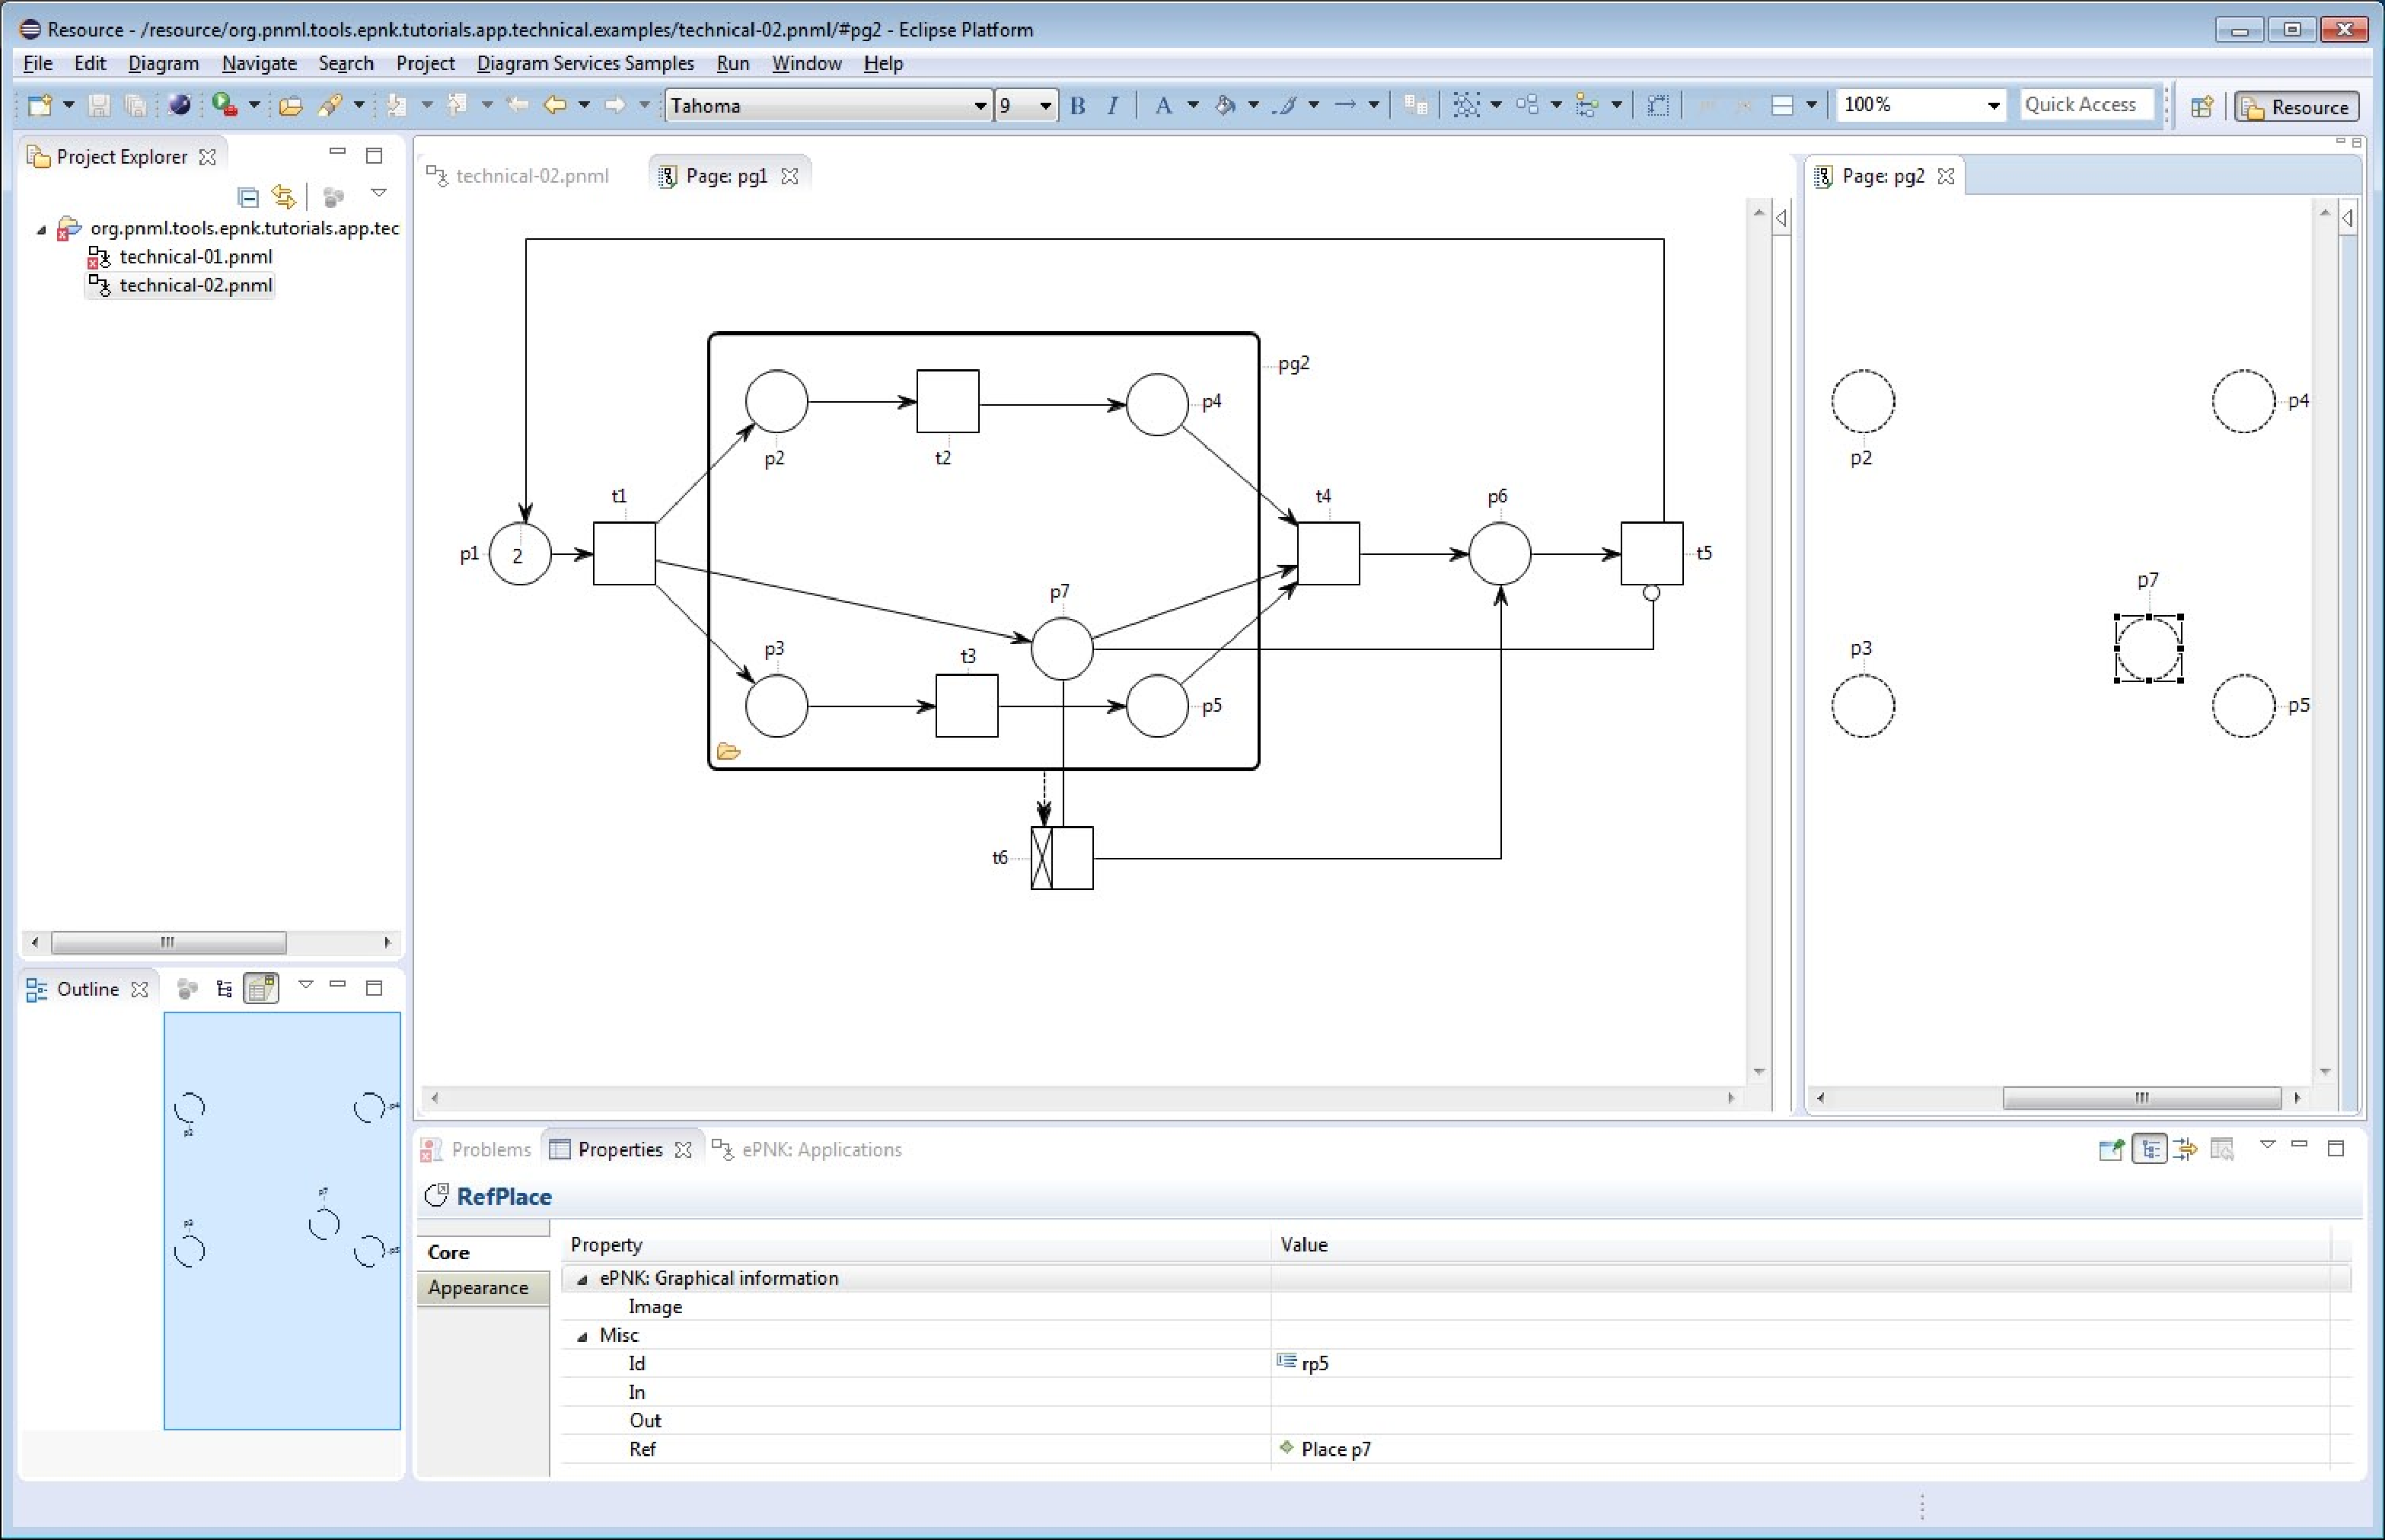
\includegraphics[scale=.34]{tutorial/TechnicalApplication1.pdf}}
  \caption{The example tool with an example of a technical net}
  \label{fig:tutorial:app1}
\end{sidewaysfigure}

In the \emph{technical net type}, we can connect \emph{places} and
\emph{transitions} with \emph{normal} arcs. As usual \emph{normal} arcs can run
from a place to a transition or the other way round. In addition, there are two
other kinds of arcs, which run from a place to a transition: \emph{read} arcs
and \emph{inhibitor} arcs. As the name suggest, a \emph{read} arc will not
change the number of tokens on the attached place; but the attached
transition can fire only, when there is at least on token on the place attached
to the other end of the read arc.
The inhibitor also does not change the number of tokens on the attached place when the transition fires. But, by contrast to the read
arc, the transition will only be allowed to fire, if there is no token on the
attached place (a token on the attached place ``inhibits'' the firing of the
transition). A \emph{read} arc is graphically represented as a line without
arrow heads on either end, but it technically runs from a place to a
transition. In our example, there is only one \emph{read} arc, running from
place $p_7$ to transition $t_6$.
An \emph{inhibitor} arc is graphically represented with a ``lollipop''
decoration at the transition end --  and the direction of the arc is from
the place to the transition. In our example, there is only one \emph{inhibitor}
arc, running from place $p_7$ to transition $t_5$.

The concepts discussed so far are all well-know concepts in Petri nets. We
will see later, that in our simulator for \emph{technical net type}, the
end-user is able to deactivate \emph{read} arcs and \emph{inhibitor} for some
simulation step -- ignoring the \emph{deactivated} arcs. There is one additional
concept in our \emph{technical net type}: these are \emph{reset} arcs, which --
just for the fun of it -- run from a page to a transition. In our example, there is one
\emph{reset} arc running from page $pg_2$ to transition $t_7$. A reset arc
does not have any effect on the enabledness of the attached transition; but,
when the transition fires, the tokens from all places contained in the attached
page will be removed. To be more precise, the tokens will be removed from the
places contained on the page and from the places to which the \emph{reference
places} on that page refer to (we say that the \emph{reference place}
\emph{resolve} to that \emph{place}).
In our example, these are the places $p_2$, $p_3$, $p_4$, $p_5$ and $p_7$ again. Graphically,
a \emph{reset} arc is represented by a dashed line with a double arrowhead.
The dashed line indicating that this arc does not prevent the transition from
firing; the double arrow head indicating that all tokens will be
removed from the places on that page.

At last, there is a minor twist\footnote
  {To be honest, we have chosen this feature only in order to demonstrate how
   to customize the graphical appearance of net objects in this tutorial.},
which is only of graphical nature. The
graphical representation of transition $t_7$ shows a cross in the left third of the
rectangle representing the transition. This indicates that this
transition does not have any \emph{normal} arc running to it. Since this
situation is sometimes not desired, it is indicated with a
special graphics; likewise, if there is no \emph{normal} arc starting at
the transition, this is graphically represented by a cross in the right
third of the transition. 

\subsection{The application}
\label{sec:tutorial:tool:application}

In addition to realizing a new net type, which then can be created and edited
in the graphical editor of the ePNK, the ePNK allows adding
\emph{application} on Petri nets. The applications could be some
analysis, simulation or verification; and the applications can visualize which
their results with a graphical feedback to the end-user, on top of the graphical
representation in the graphical ePNK editor.

In this tutorial, we discuss how to develop a \emph{simulator} for our
\emph{technical net type}, which we had introduced in
Sect.~\ref{sec:tutorial:tool:nettype}. In the following, we discuss this
simulator and its features from the end-user's point of view.

When a net or actually a page of a net of some type is open in the graphical
editor of the ePNK (and when this editor has the focus), all applications that
are defined for this net can be started by selecting the application in a small
drop down menu in the \emph{ePNK applications view}, which is indicated by
a small red circle in Fig.~\ref{fig:tutorial:app2}. In this figure, the
simulator called \emph{Technical Simulator (Tutorial)} was started already;
once started, some overlays in the graphical overlay indicate the initial
marking of the net, and also the enabled transition are highlighted. The
current marking of the net in the simulator is shown by a blue number to
the top-right of the respective place; but only places which have at least
one token hav such an annotation. This annotation for a place is also called
a \emph{marking} of the place -- to be precise, it is the \emph{current
marking} of the place -- as opposed to the \emph{initial} one which is
represented in the net itself. In Fig.~\ref{fig:tutorial:app2}, place $p_1$ has
two tokens; all the other places do not have a marking. The \emph{enabled}
transitions in the current marking are highlighted with a red overlay --
in the example, only transition, $t_1$, is enabled.

\begin{figure}[hbtp!!]
  \centerline{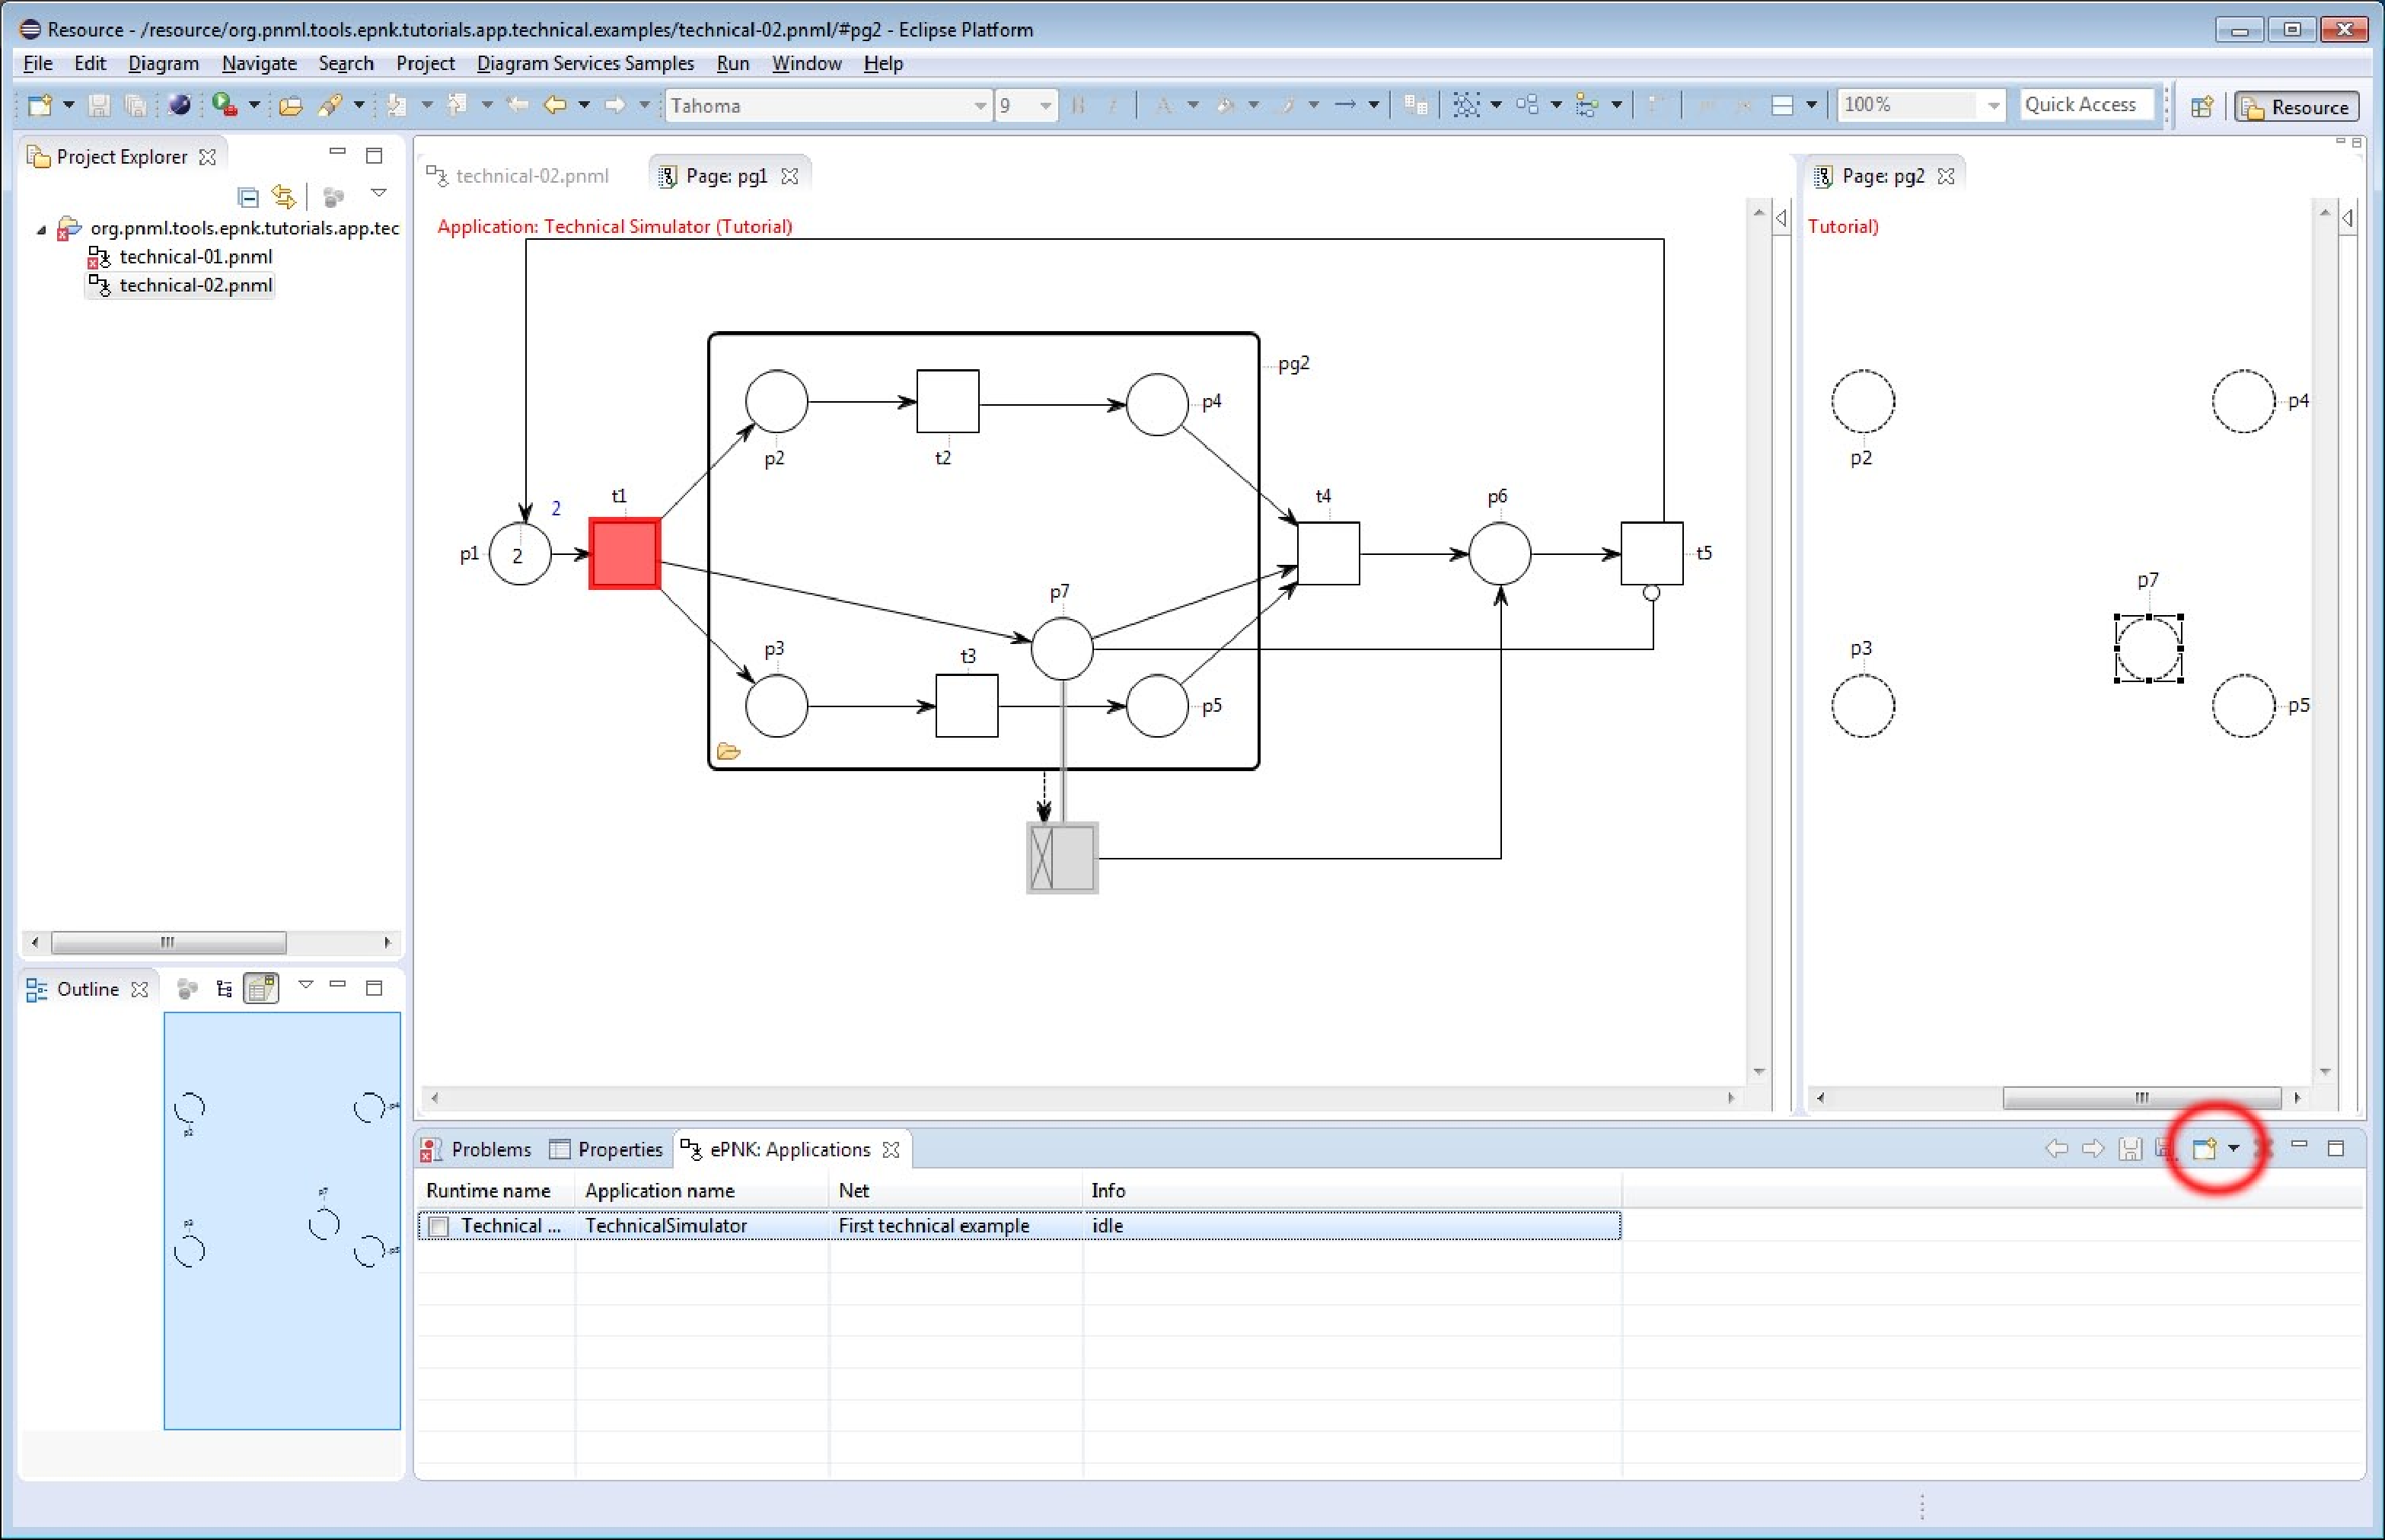
\includegraphics[scale=.24]{tutorial/TechnicalApplication2a.pdf}}
  \caption{The example net with the example simulator started}
  \label{fig:tutorial:app2}
\end{figure}

Note that, in the situation of  Fig.~\ref{fig:tutorial:app2}, also transition
$t_6$ at the bottom is highlighted with some light grey overlay and also
the read arc to place $p7$ has a light grey overlay. This indicates that, when
ignoring read and inhibitor arcs, transition $t_6$ would be enabled. We say
that this transition is \emph{weakly enabled}. By clicking on the read arc,
the end-user could choose to ignore that arc and then fire the transition. We
discuss that later.

When double-clicking on an \emph{enabled transition}, the respective transition
will \emph{fire}, the \emph{marking} of the places will change and the
\emph{enabled} transitions in the new marking will be highlighted. Figure~\ref{fig:tutorial:app3} shows
the situation after the end-user has fired (double-clicked on) the sequence
of transitions $t_1$, $t_1$, $t_2$, $t_3$, and $t_4$. In that situation, places
$p_2$, $p_3$, $p_7$ and $p_6$ have one token each (have \emph{marking} $1$), and
transitions $t_2$,  $t_3$, and $t_6$ are \emph{enabled}. Transition $t_5$ is
only \emph{weakly enabled} since the inhibitor arc from place $p_7$ to
transition $t_5$ prevents it from firing (place $p_7$ has a token).

In Fig.~\ref{fig:tutorial:app3}, you can also see another detail of the
simulator: the current marking is not only shown as an annotation of the
respective place. It is also shown as annotation of each reference place
that \emph{resolves to} the place -- as you can see for the reference places
shown on the right-hand side.
 
\begin{figure}[p!!]
  \centerline{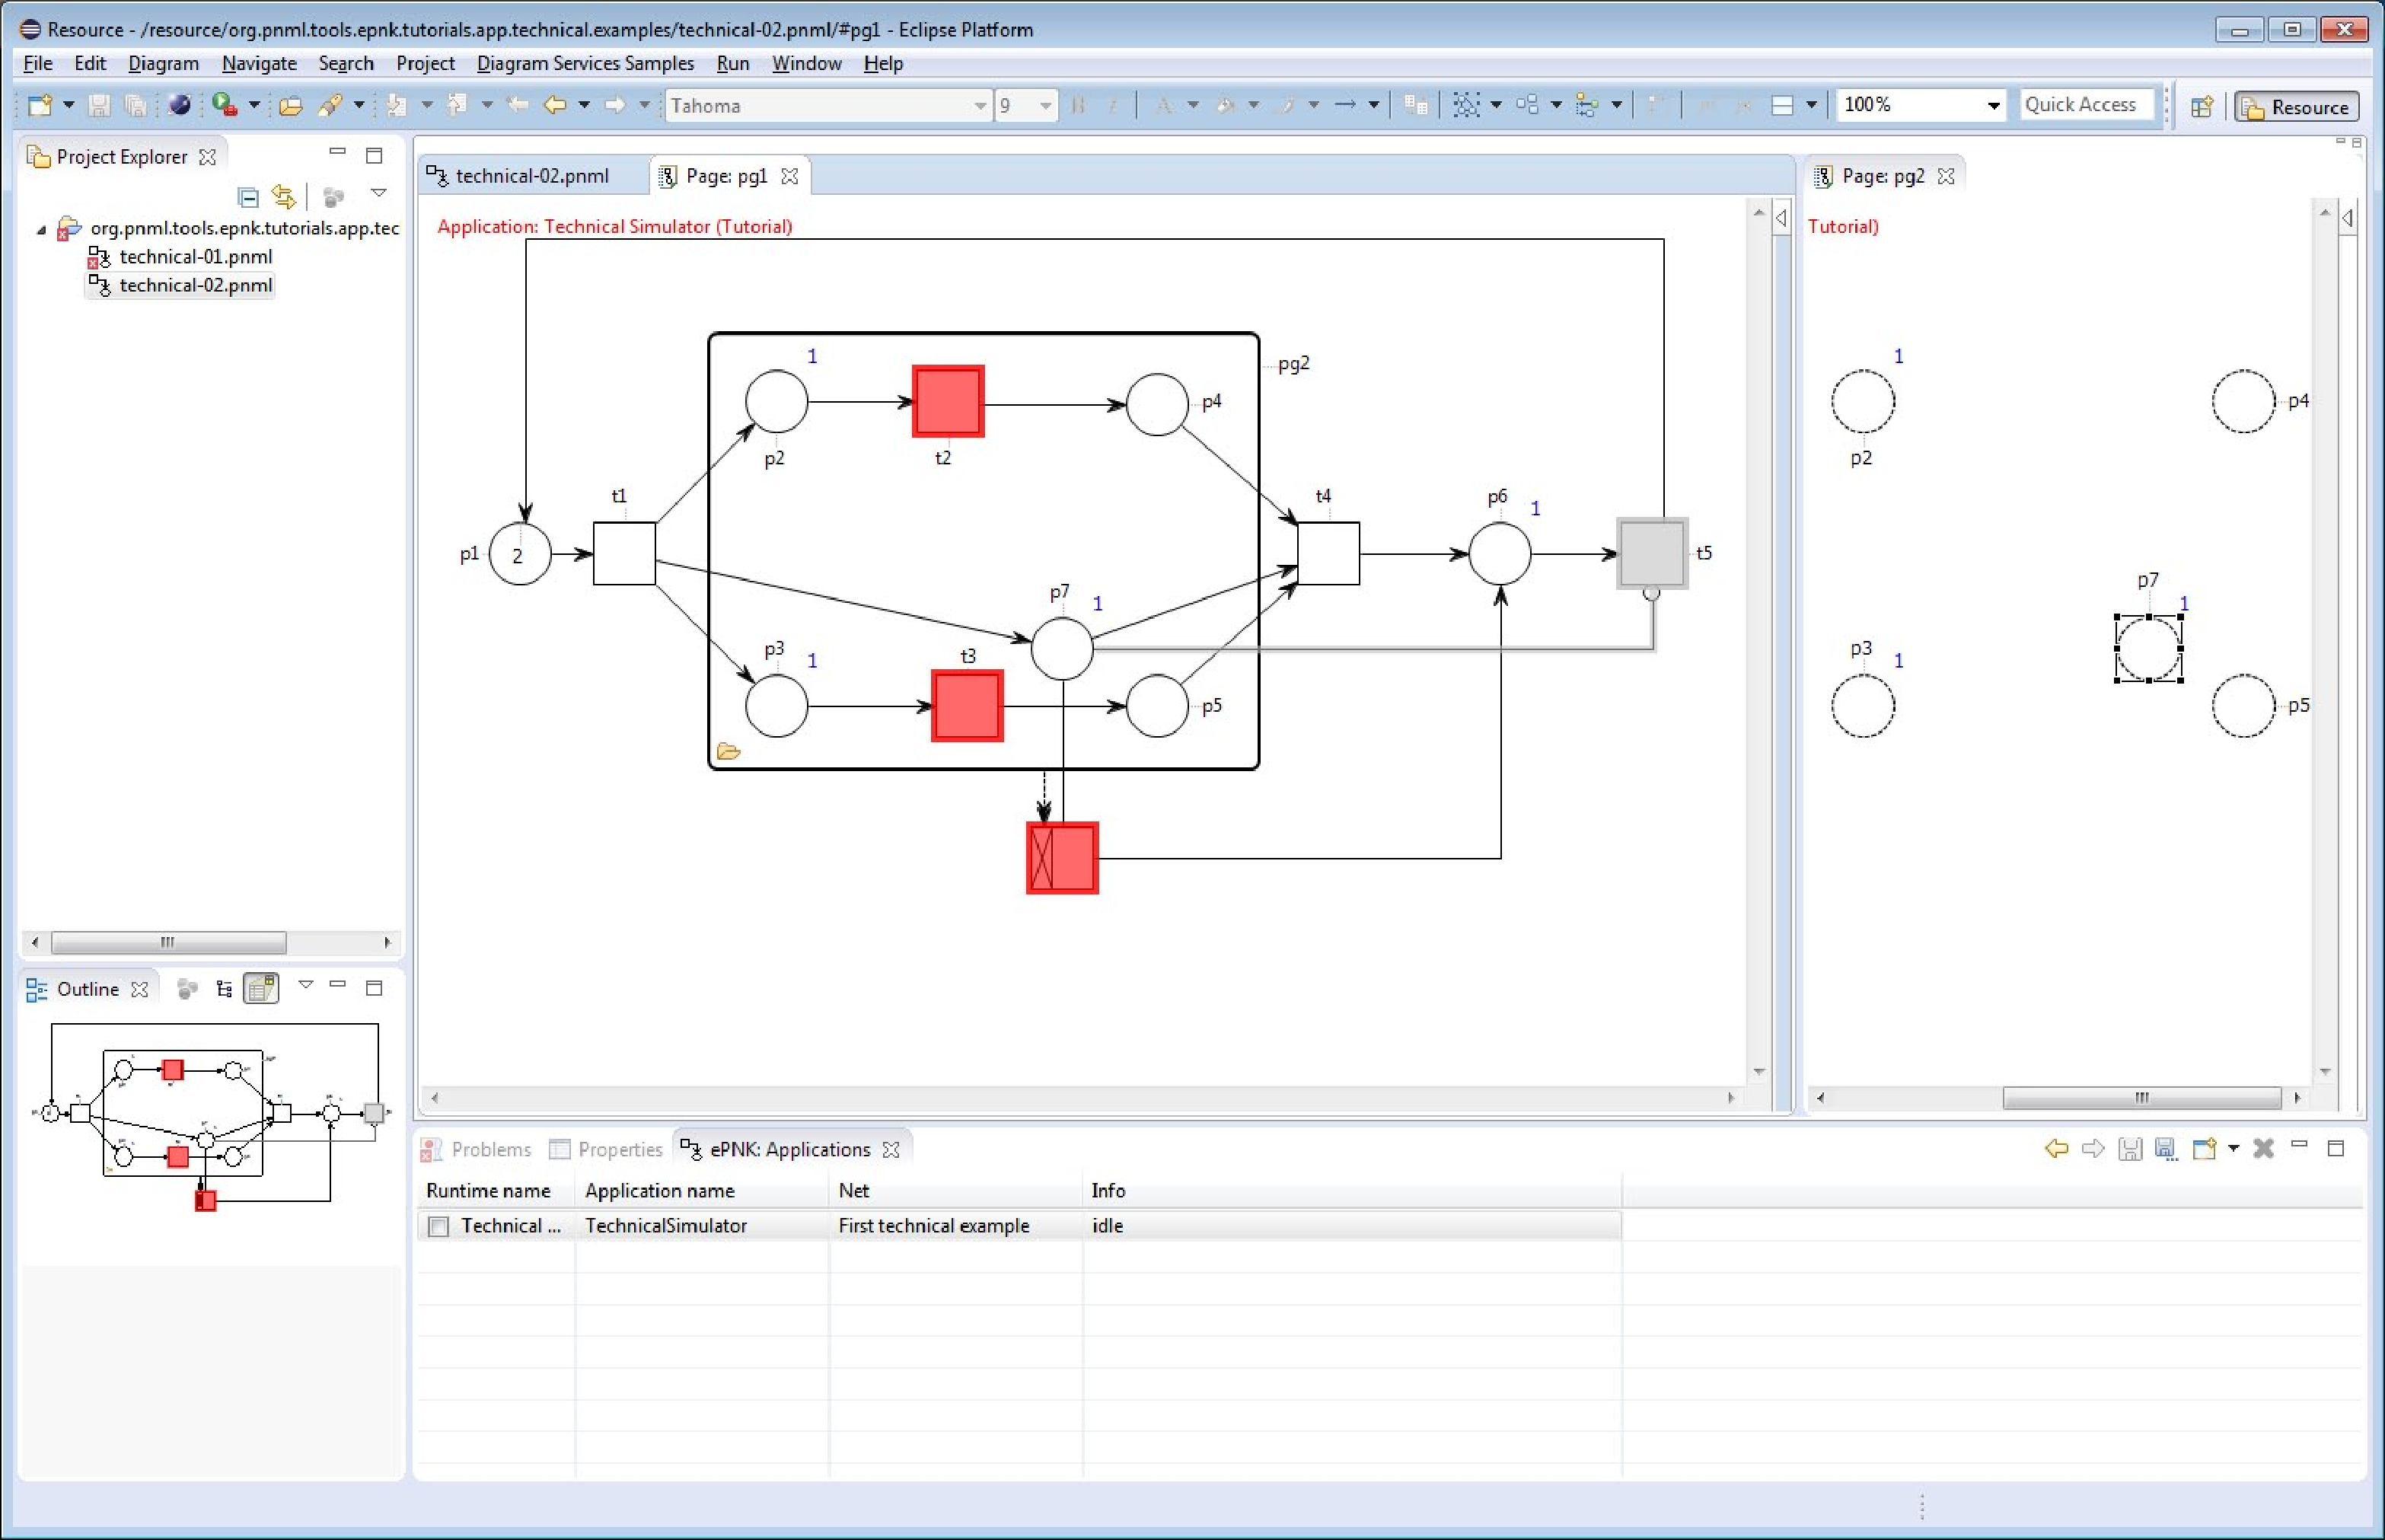
\includegraphics[scale=.24]{tutorial/TechnicalApplication3.pdf}}
  \caption{The simulator after firing transition $t_1$, $t_1$,
  $t_2$, $t_3$ and $t_4$}
  \label{fig:tutorial:app3}
\end{figure}

\begin{figure}[p!!]
  \centerline{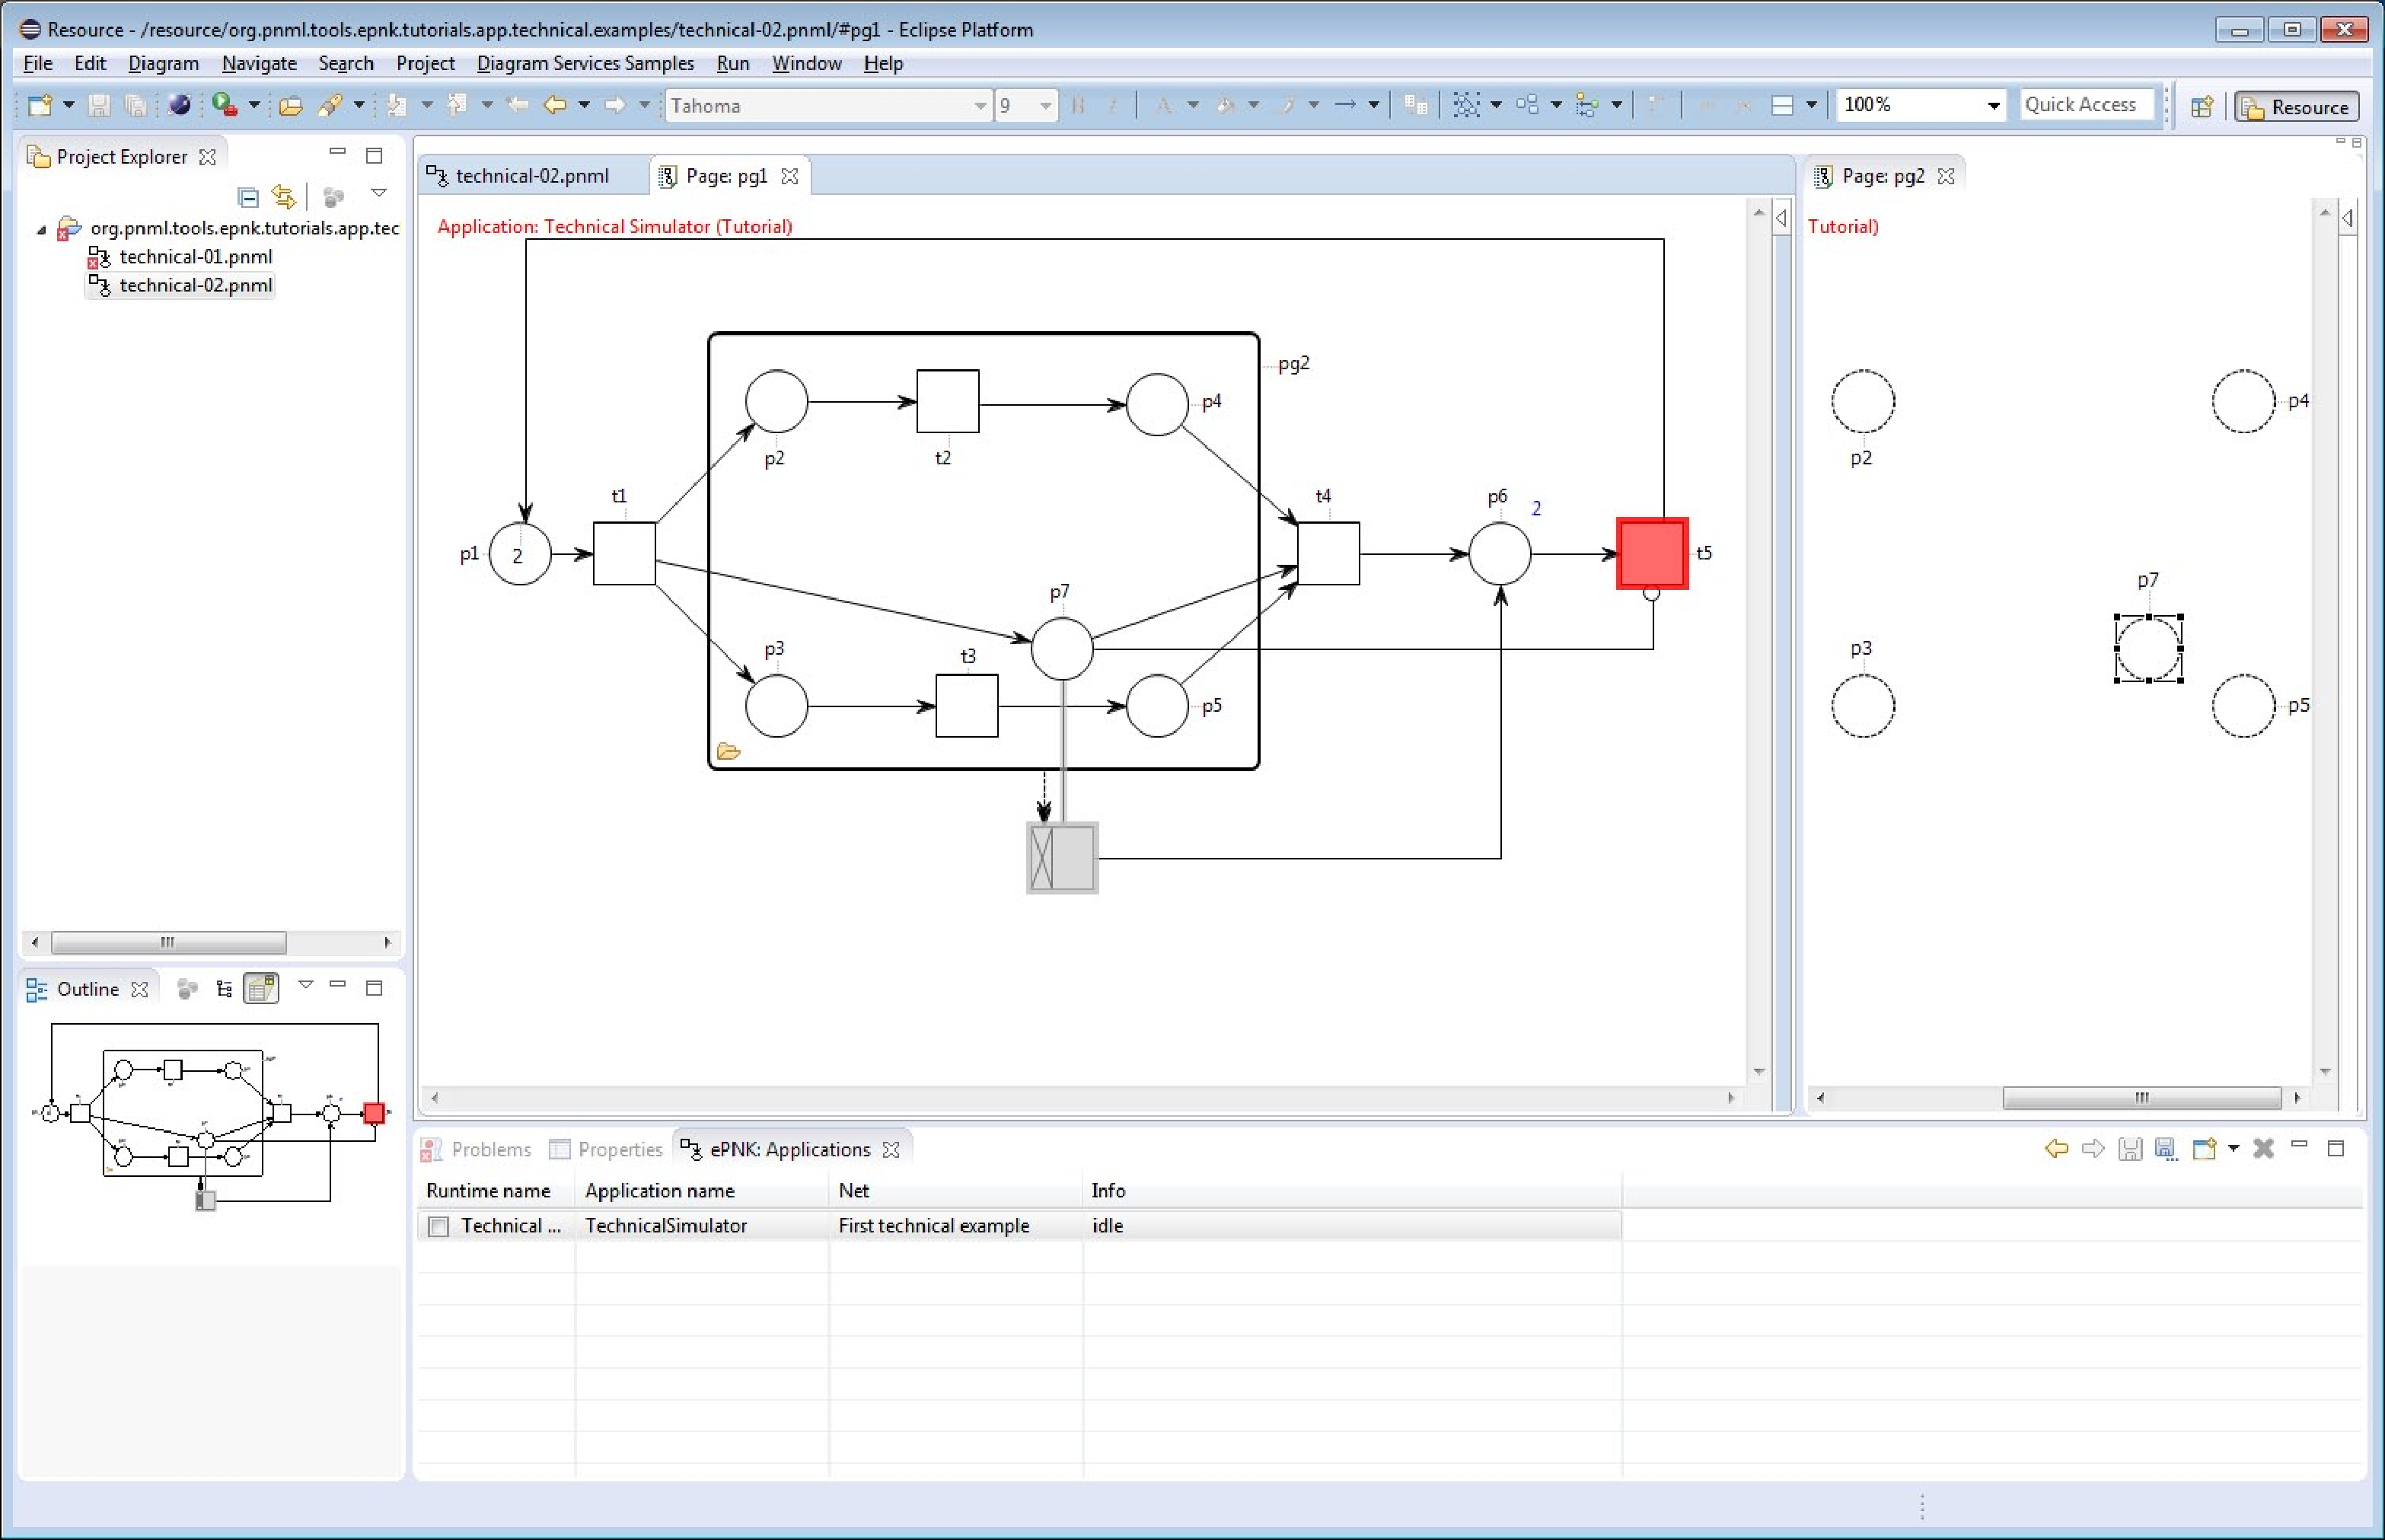
\includegraphics[scale=.24]{tutorial/TechnicalApplication4.pdf}}
  \caption{The simulator after additionally firing $t_6$}
  \label{fig:tutorial:app4}
\end{figure}

Figure~\ref{fig:tutorial:app4} shows the situation after \emph{firing}
transition $t_6$. Since this transition has a reset arc from page $pg_1$
all tokens are removed from the respective places on that page. The only
place that has tokens now is place $p_5$: it has two tokens now since
transition $t_6$ added another token.  Transition $t_5$ is enabled now,
since there is no token on place $p_7$ anymore. Moreover, transition $t_6$ is
weakly enabled.


Let us come back to the notion of a \emph{weakly enabled} transition, which is
a transition that would be enabled when ignoring conditions imposed by
\emph{read} arcs and \emph{inhibitor} arcs. In our example in Fig.~\ref{fig:tutorial:app4},
the bottom transition $t_6$ is weakly enabled only since the place at the
other end of the \emph{read} arc, place $p_7$ does not have a token. This
is indicated by the light-grey overlay of the transition and of the read arc.

The speciality of our technical net simulator is that the end-user can
deactivate \emph{read} arcs and \emph{inhibitor} arcs, by clicking on them.
Deactivated arcs will be shown with a red overlay. Once all \emph{read} arcs and
\emph{inhibitor} preventing the enabledness of a transition are
\emph{deactivated}, the transition will be enabled, indicated by a red overlay
again. Figure~\ref{fig:tutorial:app5} shows the effect of the end-user clicking
on the read arc in the situation of Fig.~\ref{fig:tutorial:app4}.
Then, the end-user can double-click on it and fire it.

\begin{figure}[hbtp!!]
  \centerline{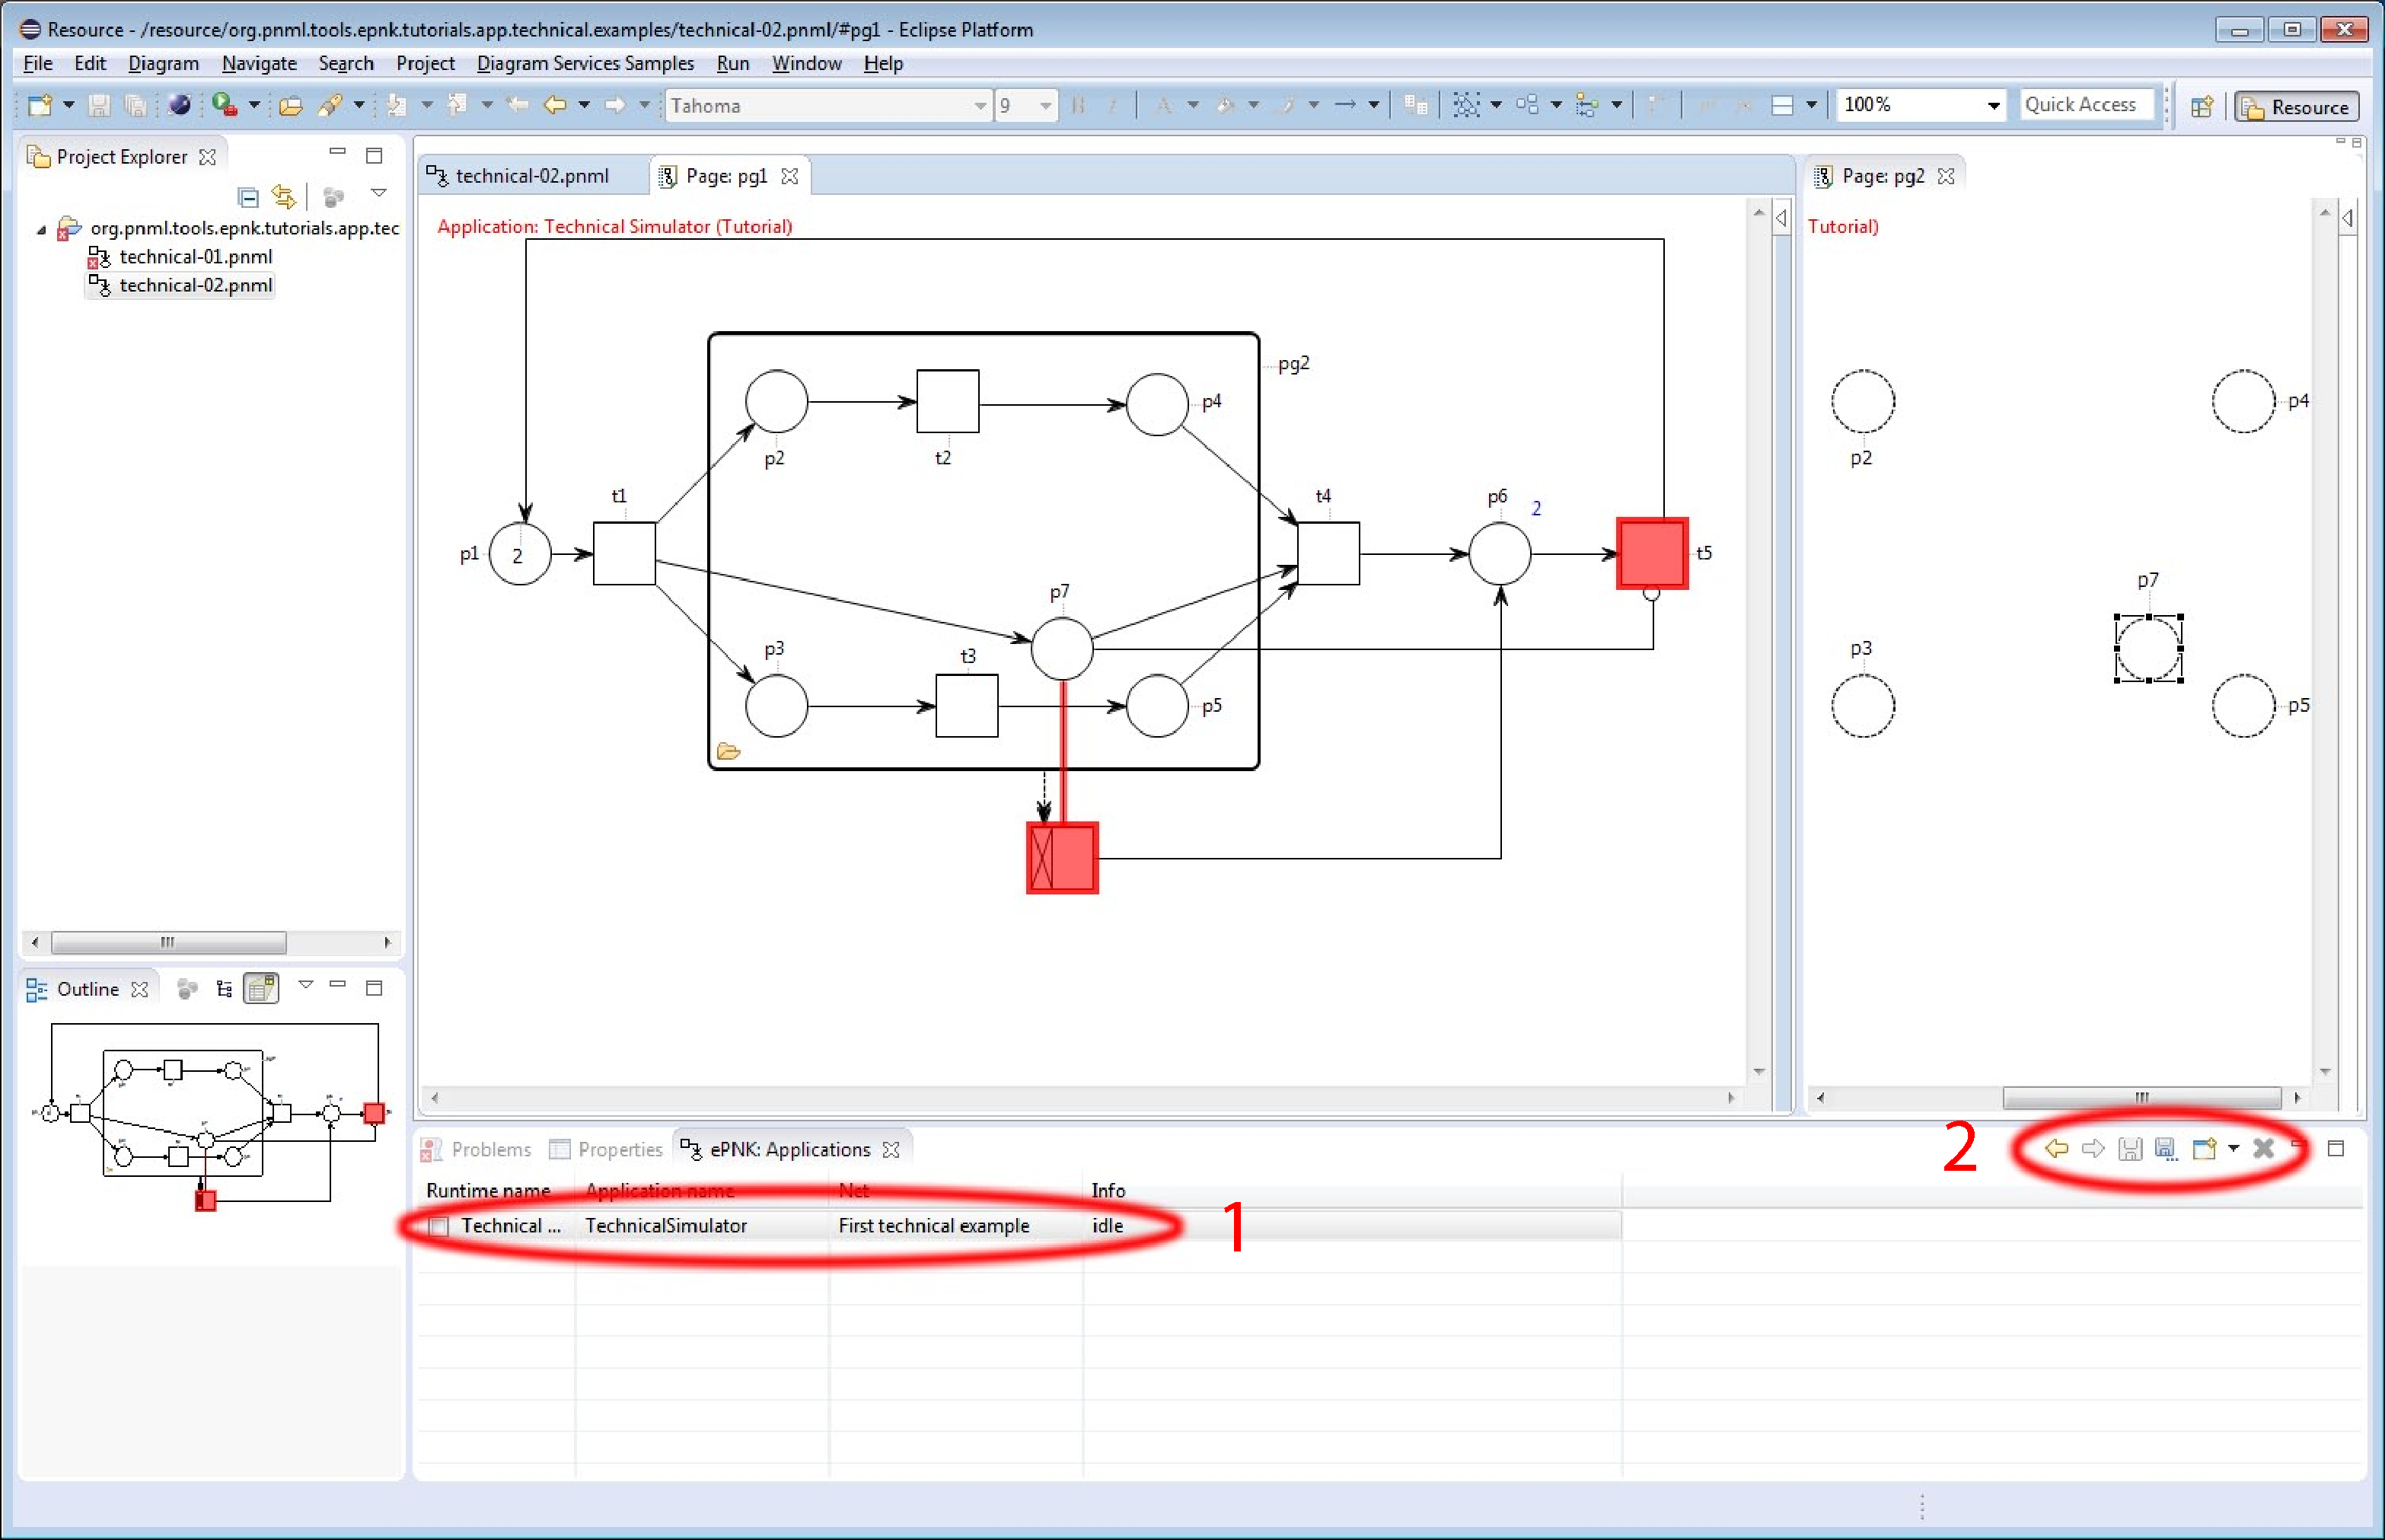
\includegraphics[scale=.24]{tutorial/TechnicalApplication5a.pdf}}
  \caption{The simulator after deactivating the read arc}
  \label{fig:tutorial:app5}
\end{figure}

At last, let us have a look at some standard features of the ePNK and the
application view. The application view shows a list of all the ePNK applications currently
running in the ePNK on some net. In the situation shown in
Fig.~\ref{fig:tutorial:app5}, only one application is running. The end-user can
select one of the running applications or un-select all applications. Then, the
visual feedback from the selected application is shown in the graphical editor
of the respective net. The end-user can also delete (shut down) applications
by selecting the check boxes of the respective applications (see line marked by
1 in Fig.~\ref{fig:tutorial:app5}) and clicking on the delete button (which
 will turn red once at least one application is selected) in the ePNK
 applications view (see the part marked with 2 in Fig.~\ref{fig:tutorial:app5}).

Note that there are also some other buttons  (see the part that is marked with 2
in Fig.~\ref{fig:tutorial:app5}). The \emph{back} and  \emph{forward} buttons
allow the end-user to go back and forth in the simulation, the disk buttons 
allows the end-user to save the current state the and firing sequence of the
simulator to a file.
Such a \emph{saved state of an application} can be loaded again, when starting
a new application with ``Load application'' in the start application
drop down menu.

\section{Conceptual steps}
\label{sec:tutorial:concepts}

In this section, we discuss the conceptual steps for realizing the tool which we
had discussed in Sect.~\ref{sec:tutorial:tool}.
The first step is the definition of our \emph{technical Petri net type}, which
basically consists of a class diagram capturing the concepts of our \emph{technical Petri net type}
and some constraints. The second step is the definition of the graphical
appearance of the features our \emph{technical Petri net type} -- in our case
the arcs and the transitions. The last step is the definition of the
\emph{simulator application} for our \emph{technical Petri nets}.

Note that, in this section, we do not discuss any technical details, how to
create the models, how to generate the code, or how to plug in the
extensions to the ePNK in order not to loose track of the overall picture.
The technical details are discussed in Sect.~\ref{sec:tutorial:technical}.

\subsection{Petri net type}
\label{subsec:tutorial:concepts:pnt}

In this section, we present a class diagram (actually an Ecore diagram),
which reflects the extensions of our \emph{technical Petri net type} as
discussed in Sect.~\ref{sec:tutorial:tool:nettype}. Basically, the extension
on top of the basic net elements, \emph{places}, \emph{transitions}, and
\emph{arcs}, are that arcs can be of kind \emph{normal}, \emph{read},
\emph{inhibitor} and \emph{reset}. In addition, places can have an
\emph{initial marking}, indicating how many tokens are on each place
initially.

\subsubsection{Petri net type definition}
\label{subsubsec:tutorial:concepts:pntd}

Figure~\ref{fig:tutorial:concepts:pntd} shows the class diagram with all the
features of our \emph{technical Petri net type}, which is called a \emph{Petri
net type definition} or \emph{PNTD} for short. This diagram refers to some classes which
are defined by the ePNK in the \emph{PNML core model}: these are the classes
shown in magenta on the left and on the top of the diagram. The other classes
shown in light cream are the definition of our \emph{technical Petri net type},
which extend the concepts of the \emph{PNML core model}.

\begin{sidewaysfigure}[hbtp!!]
  \centerline{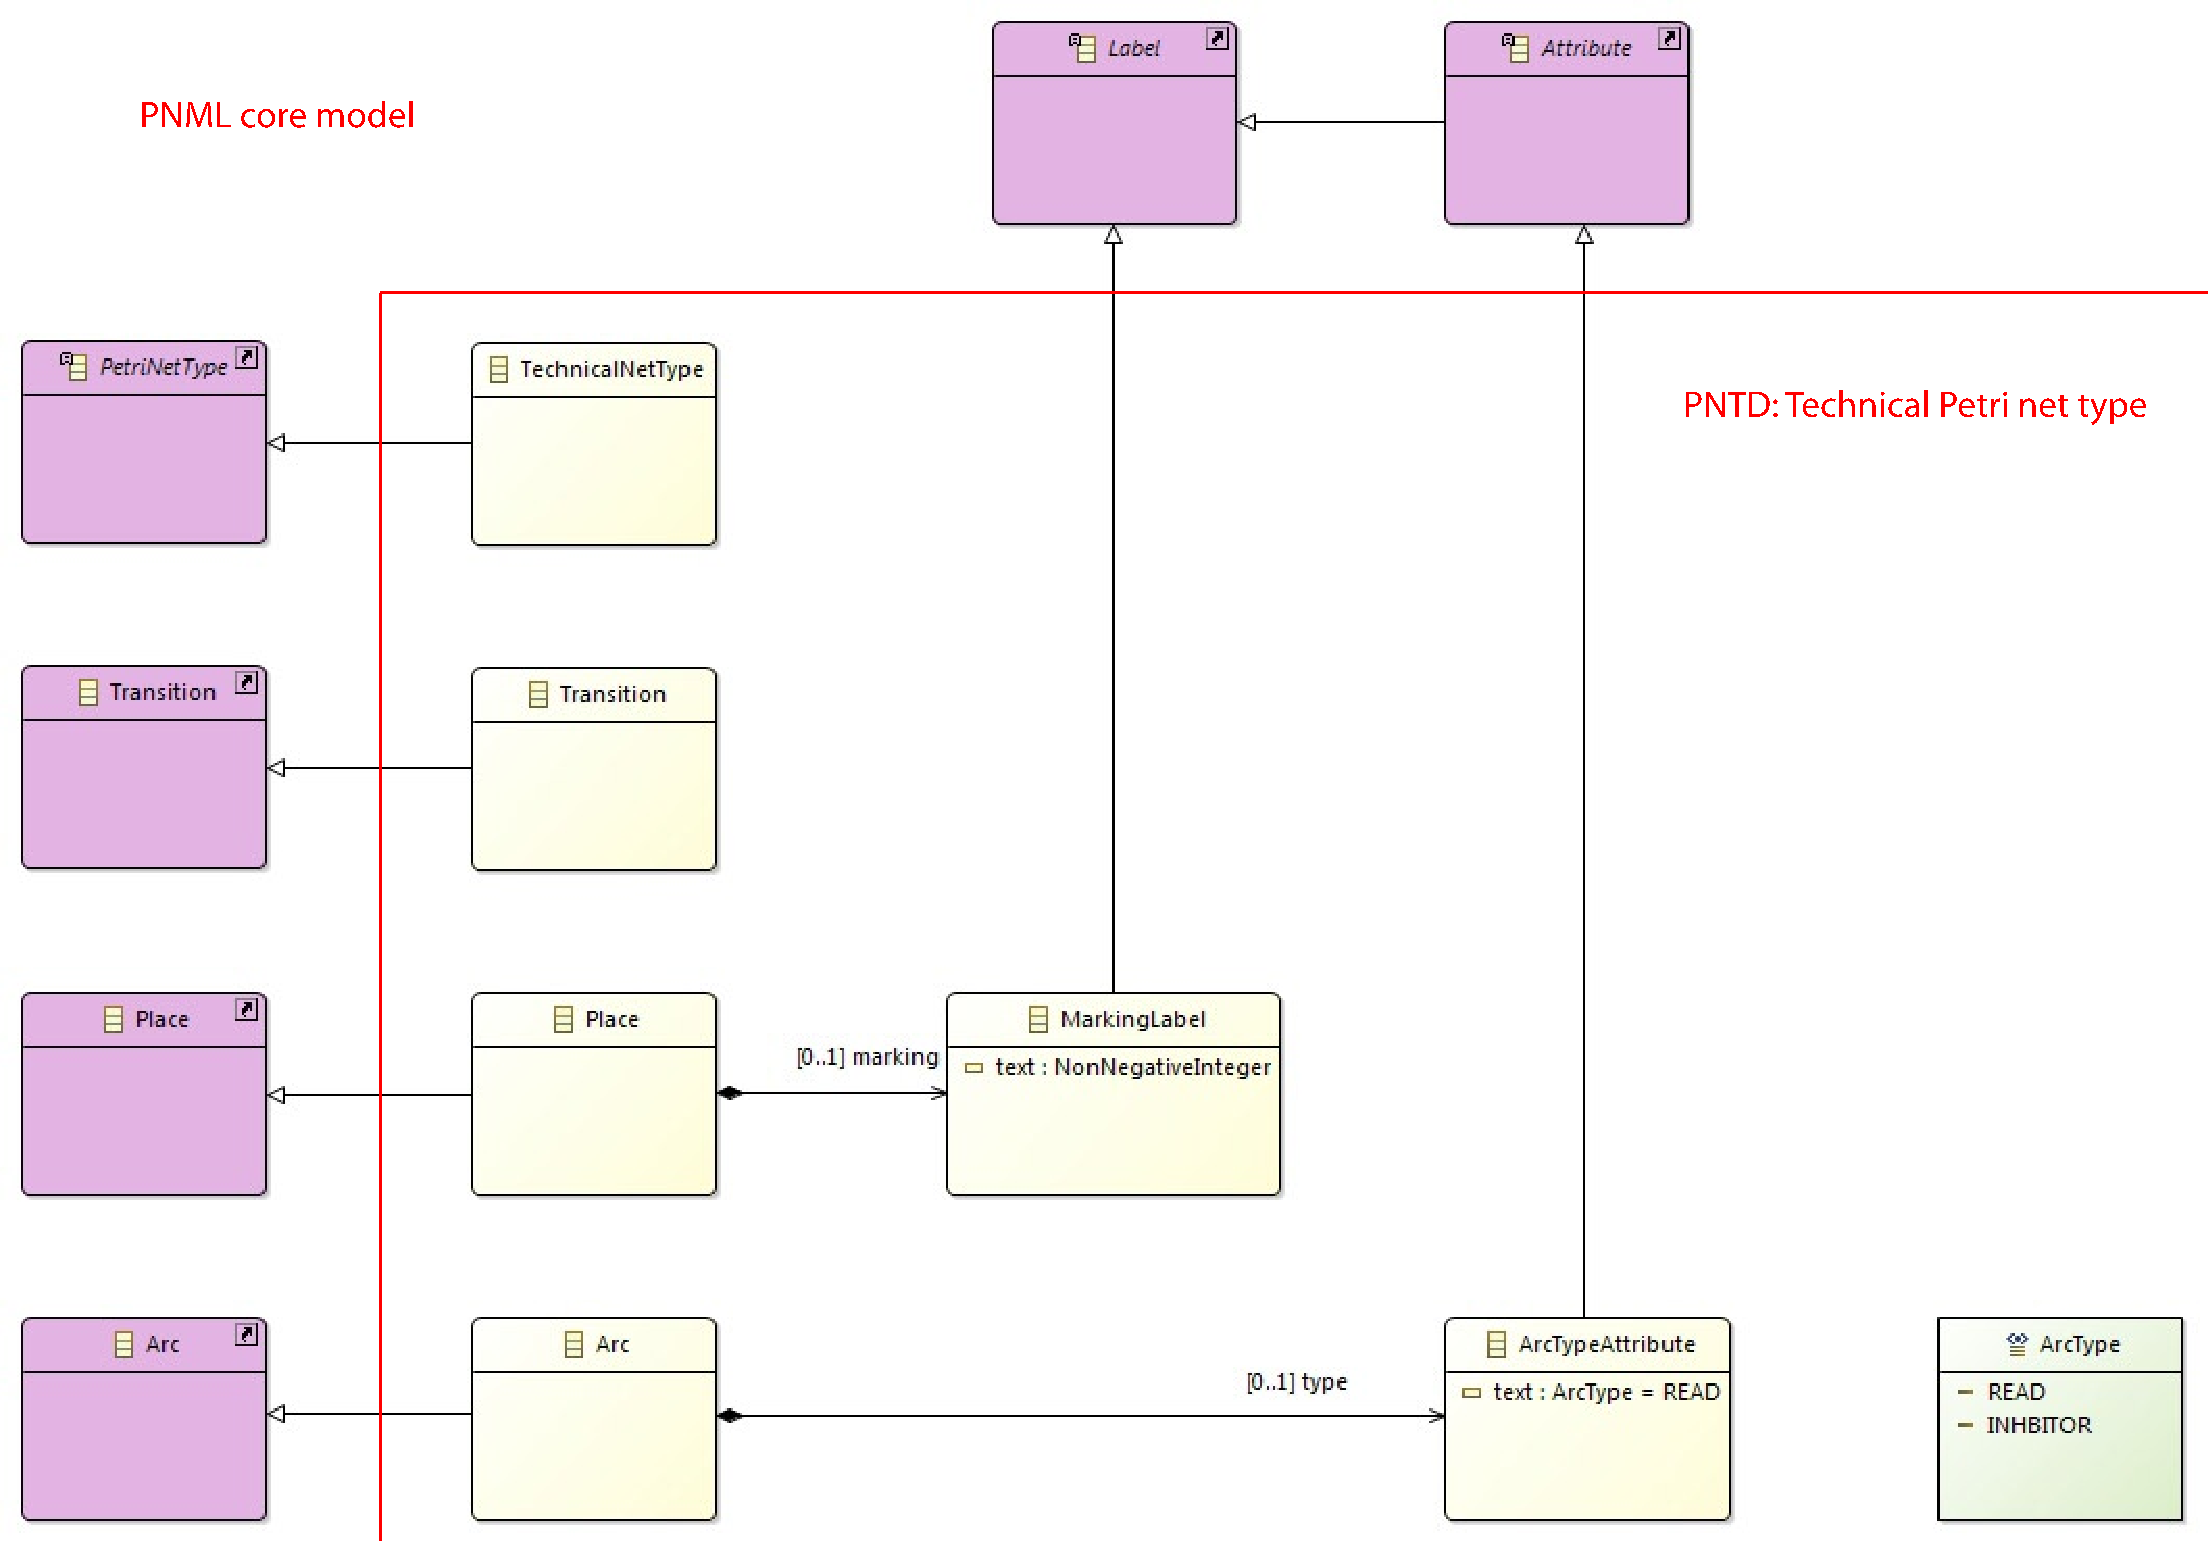
\includegraphics[scale=.45]{tutorial/technical-nets-pntd-2.pdf}}
  \caption{The Petri net type definition for the technical Petri net type}
  \label{fig:tutorial:concepts:pntd}
\end{sidewaysfigure}

There are two major extensions in our Petri net type definition in
Fig.~\ref{fig:tutorial:concepts:pntd}, the \emph{arc} and \emph{place}. Both
extend the respective concept of the PNML core model. Arcs have a concept of
\emph{ArcTypeAttribute} with an attribute \emph{text} of the enumeration type
\emph{ArcType}, which is also defined in this PNTD. \emph{Places} have
a \emph{MarkingLabel} with an attribute \emph{text} of the type
\emph{NonNegativeInteger}, which is a data type defined in the PNML core model.

The class \emph{ArcTypeAttribute} extends the class \emph{Attribute} from the
PNML core model, and the \emph{MarkingLabel} extends the class  \emph{Label}
from the PNML core model. This defines how the ePNK should handle these
additional features. A label will be graphically represented as an annotation
to the respective element. In our example, the initial marking is shown as such
a textual annotation (see Fig.~\ref{fig:tutorial:app1}) ``2'' inside the place,
this label however could be freely moved by the end-user. The type attribute
for places is not shown as an annotation of the arc; it is represented by the
graphical representation of the respective arc. It can be edited by the end-user
in the properties view, once the respective arc is selected.

Note that the classes \emph{ArcTypeAttribute} and \emph{MarkingLabel} are
associated with the class \emph{Arc} or \emph{Place} with a composition. The
name of this composition, will be the name of the respective feature and its
cardinality says how many of these features each element can have. In our
case, both cardinalities are $[0..1]$, which means that the feature is
optional and there can be at most one.

You might have realized the the enumeration \emph{ArcType} does have two
literals only: \emph{READ} and \emph{INHBITOR}. At a first glance, this might
look awkward since in the discussion of our technical Petri net type we
mentioned four different types: \emph{normal}, \emph{read}, \emph{inhibitor} and
\emph{reset}. The reason is that the arc type feature is optional, and that we
interpret a missing or not set arc type feature as \emph{normal}. Likewise
\emph{reset} is the default (or actually only) interpretation for arcs
running from a page to a transition. Therefore, it is enough that the
enumeration \emph{ArcType} represents \emph{READ} and \emph{INHBITOR}, which are
the only ones the end-user needs to set explicitly.

Note that also the \emph{marking} feature is optional. If the marking feature
is not set, the default interpretation is $0$.

In the diagram from Fig.~\ref{fig:tutorial:concepts:pntd}, there are two
additional classes defined: \emph{Transition} and \emph{TechnicalNetType},
both of which do not define any extensions on top of the PNML core model
classes they inherit from. The class \emph{Transition} would actually not be
necessary, since in our technical net type transitions do not have any
extensions. But introducing an explicit class for transitions in our PNTD allows
us to explicitly to refer to the transitions of this type. The class
\emph{TechnicalNetType}, however, is necessary: it represents the net type we
define here, and we will need it later to plug in the extension to the ePNK.

\subsubsection{Constraints}
\label{subsubsec:tutorial:concepts:constraints}

The diagram of Fig.~\ref{fig:tutorial:concepts:pntd} defines the additional
concepts of our technical Petri net type. But, is is not precise enough since
it would allow arcs running from a transition to a place to be an inhibitor
arc, which we do not want. Actually, without additional restrictions, arcs
could run between all kinds of nodes, for example between two places or between
two transitions; arcs would be even be allowed to run between two pages.

Therefore, we need to define an additional constraint that forbid arcs that
our technical net type should not have. We define an OCL constraint for
that purpose. 

\begin{figure}[htbp!]
\lstinputlisting[label=lst:tutorial:concepts:pntd:ocl,language=OCL,tabsize=2,stringstyle=\small,%
caption={OCL constraint for arcs}]%
  {code/tutorial/arc-ocl.txt}
\end{figure}

Listing~\ref{lst:tutorial:concepts:pntd:ocl} shows this  OCL constraint for
arcs: it states that an \emph{Arc} of or our technical net type can
have three different forms:
\begin{enumerate}
  \item It can run from a place to a transition. Since there also can
        be arcs between reference nodes of that kind, the requirement
        is slightly generalized to \emph{PlaceNode} and \emph{TransitionNode}.
        In that case there is no restriction of the arc's type.
        
  \item It can run from a transition to a place. For the same reasons as
        above, the requirement is slightly more general: the arc can run
        from a \emph{TransitionNode} to a \emph{PlaceNode}. For arcs from
        a transition to a place, however, the arc's type should not be set
        (i.\,e.\ it must be a \emph{normal} arc).
        
  \item It can run from a page to a transition, slightly more generalized to
        run from a \emph{Page} to a \emph{TransitionNode}. Also in that case,
        the arc's type should not be set. In this case, the arc is interpreted
        as a \emph{reset} arc.
\end{enumerate}

In order to demonstrate that constraints can also be defined in
Java, we actually introduce our example has one additional constraint: there
should not be duplicate read or inhibitor arcs between the same two nodes.
The implementation of \emph{Java constraints}, however, will first be discussed
in the technical details section (see
Sect.~\ref{subsubsec:tutorial:technical:constraints:java}).

\subsection{Graphics of the Petri net type definition}
\label{subsec:tutorial:concepts:graphics}

In Sect.~\ref{sec:tutorial:tool:nettype}, we have discussed already that some
features of our technical Petri net type should be graphically visualized in
a particular way. The type of an arc should be indicated by a dedicated
graphics for \emph{read}, \emph{inhibitor} and \emph{reset arcs} (see
Fig.~\ref{fig:tutorial:app1}). It is actually quite typical that Petri net
objects which have an attribute extension, also have a dedicated graphics for
that type of Petri net object; the reason is that the value of an attribute
is visible only in the properties view of the tool when the object is
selected, but not in the graphical representation of the net itself, unless
there is a dedicated graphical representation for it.

In our technical Petri net type, we have chosen to have a dedicated graphics
for transitions, too: transitions with no ingoing normal arc or no outgoing
should be indicated with a cross in the left or right third of the transition,
respectively, as shown for transition $t_6$ in Fig.~\ref{fig:tutorial:app1}. 

For each type of net object with a dedicated graphics, we need to implement a
\emph{Figure} class, which takes responsibility for the graphics of that
element.
Basically, there are two ways of implementing the such figures. The
first one is to change the figure by changing its configuration and graphical
attributes. In our example, we use that way for the graphical representation of
arcs. The second one is to override how the figure is actually drawn.
In our example, we use that way for the graphical representation of transitions.


Listing~\ref{lst:tutorial:concepts:graphics:arc} shows the code snippet which
configures how an arc is drawn, dependent on its type. Basically, there are
four cases: if the arc is a \emph{read} arc, both the source and the target
decorator are set to {\tt null}, so that the arc does not have any arrow
head; if the arc is an \emph{inhibitor} arc the source decorator is set to
{\tt null} and the target decorator is set to a new \emph{CircleDecoration}
which is a class provided with the ePNK; for a \emph{reset} arc, the line style is
set to dashed, and the target decorator is set to a new
\emph{DoubleArrowHeadDecoration}; at last, for normal arcs the line style is
solid, there is no source decorator, and the target decorator is a normal
\emph{ArrowHeadDecoration}, which is provided by the ePNK. If need should be,
new decoration classes could be implemented for the graphical extension. But,
this is not necessary in our tutorial example.

Note that Listing~\ref{lst:tutorial:concepts:graphics:arc} gives just a glimpse
of the respective class. We discuss more details on how to plug in this class
and how and when to properly update the graphical representation of a net object
in the technical details.

\begin{figure}[htbp!]
\lstinputlisting[label=lst:tutorial:concepts:graphics:arc,language=Java,tabsize=2,stringstyle=\small,%
caption={Arc graphics: defining appearance of acs}]%
  {code/tutorial/arc-graphics-java.txt}
\end{figure}


Listing~\ref{lst:tutorial:concepts:graphics:transition} shows the code snippet
which takes care of drawing the graphical representation of a transition --
overriding the \emph{fillShape} method. On top of drawing the figure as usual
by calling {\tt super.fillShape(graphics)}, the two conditional statements
are code for ``drawing'' the separator and a cross in the left respectively right
third of the transition using the programming mechanisms of Eclipse Draw2D, if
necessary. Also here, there are some more technical details on how to plugin the
respective class to the ePNK and how to update the graphics when needed. We
discuss this in the technical details.

\begin{figure}[htbp!]
\lstinputlisting[label=lst:tutorial:concepts:graphics:transition,language=Java,tabsize=2,stringstyle=\small,%
caption={Transition graphics: drawing the figure}]%
  {code/tutorial/transition-graphics-java.txt}
\end{figure}

\subsection{The simulator application}
\label{subsec:tutorial:concepts:app}

At last, we need to define the simulator application, which allows the end-user
to simulate the technical nets, and which visualizes the current state of
the Petri net and the currently enabled transitions graphically on top
of the net shown in the graphical editor.

\subsubsection{Runtime annotations}
\label{subsubsec:tutorial:concepts:app:annot}

In order to separate concepts from the actual graphical representation, the
ePNK allows us to define \emph{annotations} for nets, which reflect runtime
information for our application. In our case, this would be the current state of
the simulator, information on the enabled transitions and activated and deactivated
arcs.

Like for the definition of a Petri net type, the conceptual annotations of
an application can be defined by a class diagram, which extends some basic
annotation concepts provided by the ePNK.
Figure~\ref{fig:tutorial:concepts:app:annot:model} shows this model, where
the two classes shown on the top and in magenta represent the based concepts
from the ePNK: \emph{object annotations} is any form of annotation of any
Petri net object; \emph{textual annotations} is information that typically
is represented by a text instead of a graphical overlay.

The classes represented in light cream are the \emph{annotations} needed for our
simulator.
\emph{EnabledTransition} is an annotation for weakly enabled
transition -- the value of attribute \emph{enabled} indicates whether 
the transition is \emph{truly} enabled. \emph{Marking} represents the
current marking of a  place (i.e.\ the number of tokens on that place). The
actual value is represented by its attribute \emph{value}. Since the value
should be shown as textual annotation, this class extends not only the
\emph{ObjectAnnotation} but also \emph{TextualAnnotation} of the ePNK.

At last \emph{InvolvedArc} is an annotation for arcs, which indicate arcs
of a weakly enabled transition that prevent the enabledness of this
transition. This way, the end-user can toggle whether the arc is \emph{active}
or not. The status of this user's selection is represented by attribute
\emph{active}.

In order to keep track of the arcs involved in an enabled transition, there
are two compositions from \emph{EnabledTransition} to \emph{InvolvedArc}: one
for the transition's incoming arcs and one for the outgoing arcs (the outgoing
arcs are actually not used in our example). This way, it is possible to navigate
between enabled transition annotations and the involved arc annotations.

Note also that there is a bidirectional relationship between the
\emph{EnabledTransition} itself. The reason is that a single transition can have
many reference transitions referring to it. In our simulator, also the
reference transitions that resolve to an enable transition should be marked as
enabled. The reference \emph{resolve} represents the transition, the reference
\emph{ref} represents all the reference transitions. We will see later in more
detail how our simulator uses this information.

\begin{figure}[hbtp!!]
  % \centerline{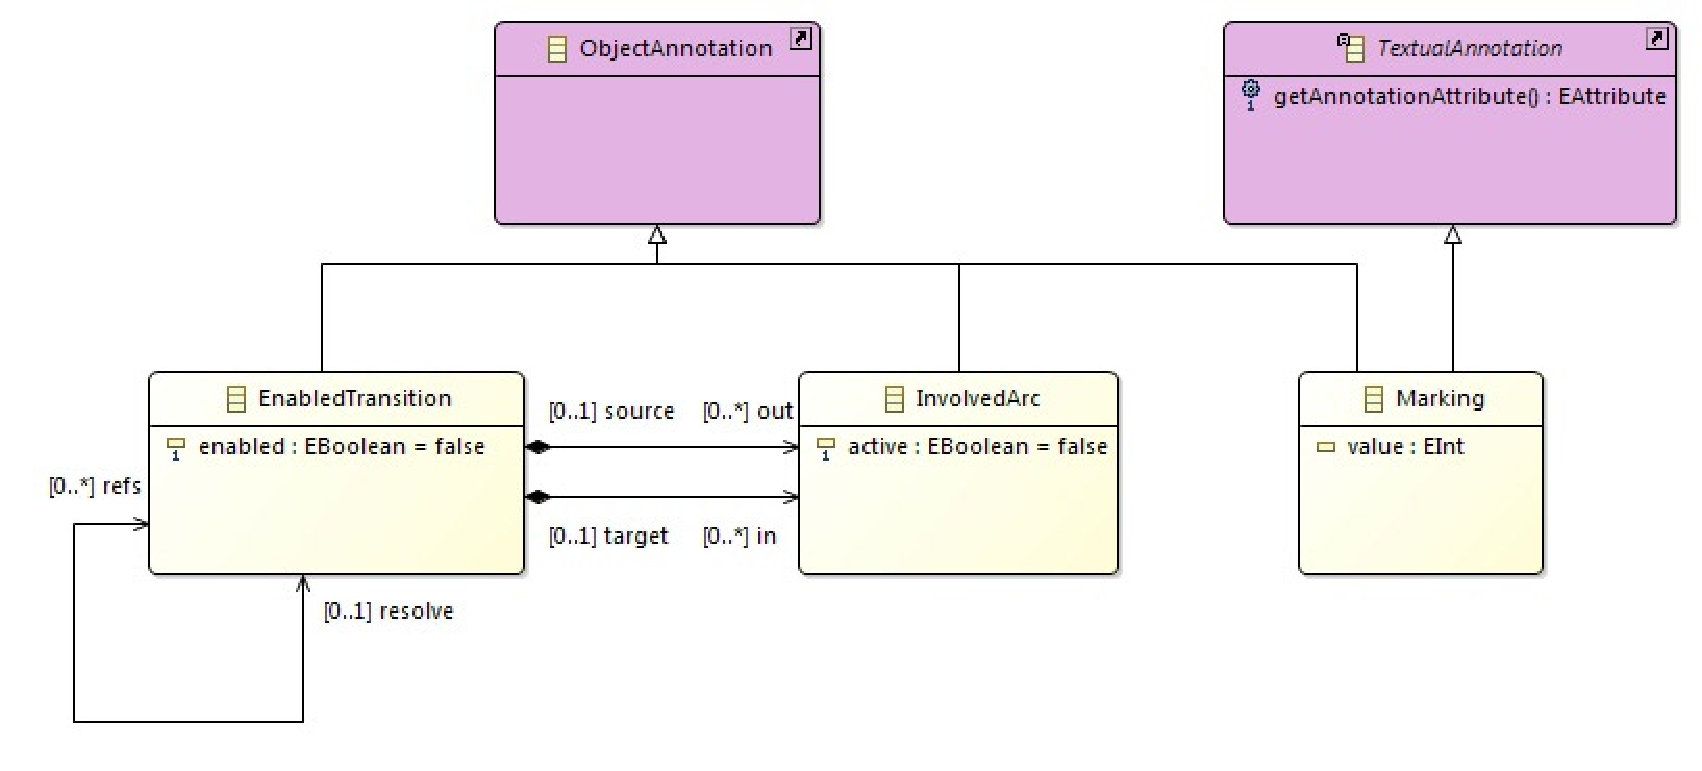
\includegraphics[scale=.45]{tutorial/techsimannotations.pdf}}
  \centerline{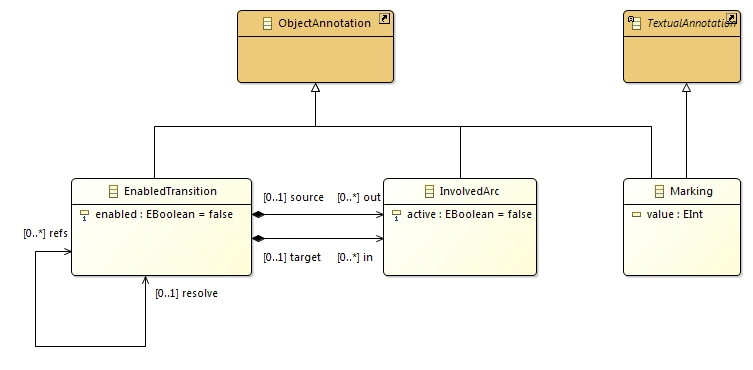
\includegraphics[scale=.45]{tutorial/techsimannotations.jpg}}
  \caption{Simulator: annotations model}
  \label{fig:tutorial:concepts:app:annot:model}
\end{figure}

An \emph{PNK application}, basically, consists of a list of
\emph{net annotations}, each of which which in turn consists of some
\emph{object annotations}.
Moreover, there always is a \emph{current} net annotation, which for example
represents the current state of the simulator. In our example, a net annotation represents
the current markings of the places plus the enabled transitions and the involved
arcs and their state.

In order to visualize the current state of an ePNK application in the graphical
editor, an ePNK application uses one or more \emph{presentation handlers}. A 
\emph{presentation handler} tells, for each annotation, how it should be
visualized in the net.
In order for end-user to be able to interact with the simulator via
the annotations, an ePNK application uses one ore more \emph{action
handlers}.
An \emph{action handler} defines how the simulator should react to a user interaction (mouse
press, mouse release, and mouse double click). This could for example, be
firing a transition by updating the net annotations, or toggling the active status 
of an involved arc. We discuss more details in the technical parts of
this tutorial.

Here we briefly discuss the main ingredients and functionality that
needs to be implemented for our simulator (and actually most kinds of
simulators):
\begin{enumerate}
\item We need some data structure or dedicated class, which represents 
      a \emph{marking of the net}, which basically is a mapping from places to
      integers.
\item We need a method, which computes the \emph{initial marking of the net}
      from a net model.
\item We need methods, which, for a given marking and some transition, computes
      whether the transition is \emph{enabled}, and which are the \emph{involved
      arcs}.
\item We need a method which for a given marking and a given enabled transition
      computes the marking which is the result after \emph{firing the
      transition in the given marking}. 
\item We need a method, which from a marking \emph{computes a net annotation}.
      representing the marking of the places as well as the enabled transitions,
      and the involved arcs.
\end{enumerate}

We discuss in the technical steps how the above methods can be combined
into a complete simulator using also the presentation handlers and action
handlers.

\section{Technical steps}
\label{sec:tutorial:technical}

In Section~\ref{sec:tutorial:concepts}, we have discussed the major conceptual
steps for realizing a Petri net type definition (PNTD) for our technical net
type and simulator for them based on the ePNK.

In the following sections, we discuss all the technical details, some subtle
issues concerning tooling, and possible problems that might occur on the way,
and how to deal with them. We start with some installation information in
Sect.~\ref{sec:tutorial:technical:install} and how to install the project
implementing the extensions discussed in this tutorial in your Eclipse workspace.
Then, we go through the steps which we discussed in
Sect.~\ref{sec:tutorial:concepts} in some more detail, discussing the models and
the source code of the Eclipse projects.

Note that the tricky issues and problems are sometimes not in the resulting
projects, models or code, but in how to actually create, configure, and
manipulate them. Therefore, we also discuss how to actually create
and edit some of the artifacts in the Eclipse IDE (using the Eclipse package
which is pre-configured for working with models: \emph{Eclipse Modeling Tools}).


\subsection{Installation}
\label{sec:tutorial:technical:install}

We begin with discussing how to install Eclipse, the ePNK and the source code
for the technical example, and how to start and use it.

\subsubsection{Eclipse}
\label{sec:tutorial:technical:install:eclipse}

Before you can work with the ePNK, you need to install Java and Eclipse on your
computer. When using the ePNK as a developer and not only as an end-user, it is
recommended that you install the \emph{Eclipse Modeling Tools} package of
Eclipse. The ePNK was testes with Eclipse Mars and you can find and download the
Mars Eclipse Modeling Tools package from the Eclipse Modeling Tools web site for
Mars:
\url{http://www.eclipse.org/downloads/packages/eclipse-modeling-tools/mars2}.
You might also use the latest version of Eclipse Modeling Tools package of the
latest version of Eclipse (currently Neon), but the ePNK has not yet been tested
under Eclipse Neon yet.

In this tutorial, we also use OCL constraints. Therefore, it is recommended that
you install the ``OCL Examples and Editors SDK'' feature. You can do that
by starting your new version of Eclipse after you have installed it and by 
selecting ``Install New Software...'' in the ``Help'' menu. In the opened 
``Install'' dialog, you should choose the default update site in the ``Work with''
field\footnote
  {For Eclipse Mars, that update site would be
   \url{http://www.eclipse.org/downloads/releases/mars}.}
and type ``OCL'' in the field below. After a while, the feature ``OCL Examples
and Editors SDK'' should show up as an available feature in category
``Modeling''. Select this feature and follow through the installation process
and restart Eclipse.

\subsubsection{ePNK}
\label{sec:tutorial:technical:install:epnk}

After you have installed and started Eclipse, you need to install the ePNK
version 1.1 from the ePNK update site at
\url{http://www2.compute.dtu.dk/~ekki/projects/ePNK/1.1/update/}. You can
do that as discussed before by selecting ``Install New Software...'' in the
``Help'' menu; then, select
\url{http://www2.compute.dtu.dk/~ekki/projects/ePNK/1.1/update/} % \hspace{0em% plus 1em} 
as update site and install all features of the ePNK. Make sure that
you select the newest features of the ePNK -- \url{org.pnml.tools.epnk.core} should have version number 1.1.2 or higher.

Make sure that, in the ``Install'' dialog, the checkbox ``Contact all update
sites during install to find required software'' is checked. This makes sure that
all the extensions that the ePNK needs to run will be installed too. Then,
follow through the installation process. Note that you might be asked to confirm the
installation of unsigned features.

\subsubsection{Import of example projects}
\label{sec:tutorial:technical:install:example}

The Eclipse projects discussed in this tutorial are also available online. You
can download them as exported Eclipse projects from the ePNK update site:
\url{http://www2.compute.dtu.dk/~ekki/projects/ePNK/1.1/tutorials/ePNK-app-tutorial.zip}.
In order to install these projects into your workspace, download the above file,
and save it somewhere on your computer. Then, right-click in the project
explorer of your Eclipse workspace, and select ``Import...''; in the opened
''Import'' dialog select ``Existing Projects into Workspace'' from category
``General''; in the subsequent dialog, select ``Select archive file'' and,
by using the ``Browse...'' button, navigate to the file you had downloaded
before. Once you have chosen this file, you should see four Eclipse projects;
select all of them and ``Finish'' the import.

After that, you should see the four Eclipse projects in your Eclipse workspace,
and after building the workspace, there should not be any errors shown in your
workspace. In order to test whether these projects where correctly installed
and built, you should start another instance of your Eclipse (the so-called
\emph{runtime workbench} as opposed to the Eclipse which you have started
already, which is called \emph{development workbench}).

The first time you start up a new \emph{runtime workbench}, you need to create
a new \emph{run configuration} in your development workbench. To this
end, choose the ``Run'' symbol in the toolbar and select ``Run configuration'',
which starts a ``Create, manage and run configurations'' dialog; in this
dialog, choose ``Eclipse Application'' and click on ``New launch
configuration'', enter a name for this configuration (e.\,g.\ ePNK Tutorial),
and then click on ``Apply'' or ``Run''. After some time, a new instance of
Eclipse should start up (the \emph{runtime workbench}) -- in this instance, the
Eclipse tutorial projects that you just have imported to your workspace are
installed and running.

In order to test whether the installed projects are working fine, you should
import a project with a Petri net example -- actually it is the one shown
in Fig.~\ref{fig:tutorial:app1}. You can obtain this project from
\url{http://www2.compute.dtu.dk/~ekki/projects/ePNK/1.1/tutorials/ePNK-app-tutorial-example.zip}.
Import it to the workspace of your Eclipse runtime workbench as discussed
before. Once you have imported it, open the \emph{PNML document} {\tt
technical-02.pnml} by double-clicking on it\footnote
  {If double-clicking does not work, right-click on it and select ``Open
  with...'' and then selecting ``PNML Editor" from ``Others...''}.
Then open the elements until you reach a page and double click on the page.
On this page, a graphical editor should start up -- after a while. Once this
editor opened, open the ``ePNK: Applications'' view (using the ``Show view''
menu in the ``Windows'' menu.) In the ``ePNK: Applications'' view, use the
start application drop down menu (see red circle in
Fig.~\ref{fig:tutorial:app2}) and select ``Technical Simulator (Tutorial)'',
which should start up as shown in Fig.~\ref{fig:tutorial:app2} with
transition $t_1$ marked as enabled. You can now play around with firing
transitions by double-clicking on them as discussed in
Sect.~\ref{sec:tutorial:tool:application}. Note that you can also interact
with the arcs which are marked grey or red in order ot toggle their activation
status.

Once this works, you can shut down the simulator application, by selecting the
checkbox in front of it and then pressing the ``delete'' button.

If this works, the example projects are properly installed and you can continue
with the next technical step of the tutorial in
Sect.~\ref{sec:tutorial:technical:pntd}. For now, you can shut down (close) your
runtime workbench (the one with the example of the technical Petri net, which
you had simulated).

Note that when you want to start up a runtime workbench the next time, you do
not need to create another \emph{run configuration}. Just click on the
``Run as..'' (launch) button next time you want to start a runtime workbench.
 
In the following sections, we discuss the four projects which implement
our \emph{technical Petri net type}, its graphical representation, and the
simulator in more detail. Moreover, we discuss how you would create these
projects and some of the artifacts from scratch in the Eclipse IDE.

Note that all the example code discussed in this tutorial is taken from these
projects. Sometimes, we deletes import statements, comments or compacted the
code a bit for the discussion. You will find the source code for all listings
discussed in this tutorial in these projects for more details.

\subsection{PNTD}
\label{sec:tutorial:technical:pntd}

We start with discussing the project {\tt
org\qnsep{}pnml\qnsep{}tools\qnsep{}epnk\qnsep{}tutorials\qnsep{}app\qnsep{}pntd},
which defines the \emph{Petri net type definition} for our \emph{technical net type},
which we had conceptually discussed in
Sect.~\ref{subsubsec:tutorial:concepts:pntd}.

\subsubsection{Ecore model}
\label{subsec:tutorial:technical:pntd:ecore}

The class diagram defining the concepts of our \emph{technical net type},
which we had discussed in Sect.~\ref{subsubsec:tutorial:concepts:pntd} already,
can be found in the file {\tt technical\qnsep{}ecore} in folder {\tt model} of
\emph{EMF project} {\tt
org\qnsep{}pnml\qnsep{}tools\qnsep{}epnk\qnsep{}tutorials\qnsep{}app\qnsep{}pntd}.
It is actually an Ecore model, which is EMF's ``lightweight version'' of class diagrams.
You can inspect it with the \emph{Ecore Model Editor}, which is a simple tree
editor. Typically, you can do this by double-click on this file in the Package
explorer of the Eclipse development workspace.

Figure~\ref{fig:tutorial:technical:pntd:ecore-tree} shows the Eclipse
development workspace with the Ecore model for the technical net type
opened in the tree editor. You can also see that this model is actually
referring to elements of the \emph{PNML Core Model} which it extends; parts of
this model can be seen at the bottom of the editor. You can also see the
attributes of the defined package in the properties view: its name
``technical'', its unique URI, which we have chosen for this package
``http://epnk.tools.org/tutorials/app/technical'', and its name space prefix
``tech''.

\begin{figure}[hbtp!!]
  % \centerline{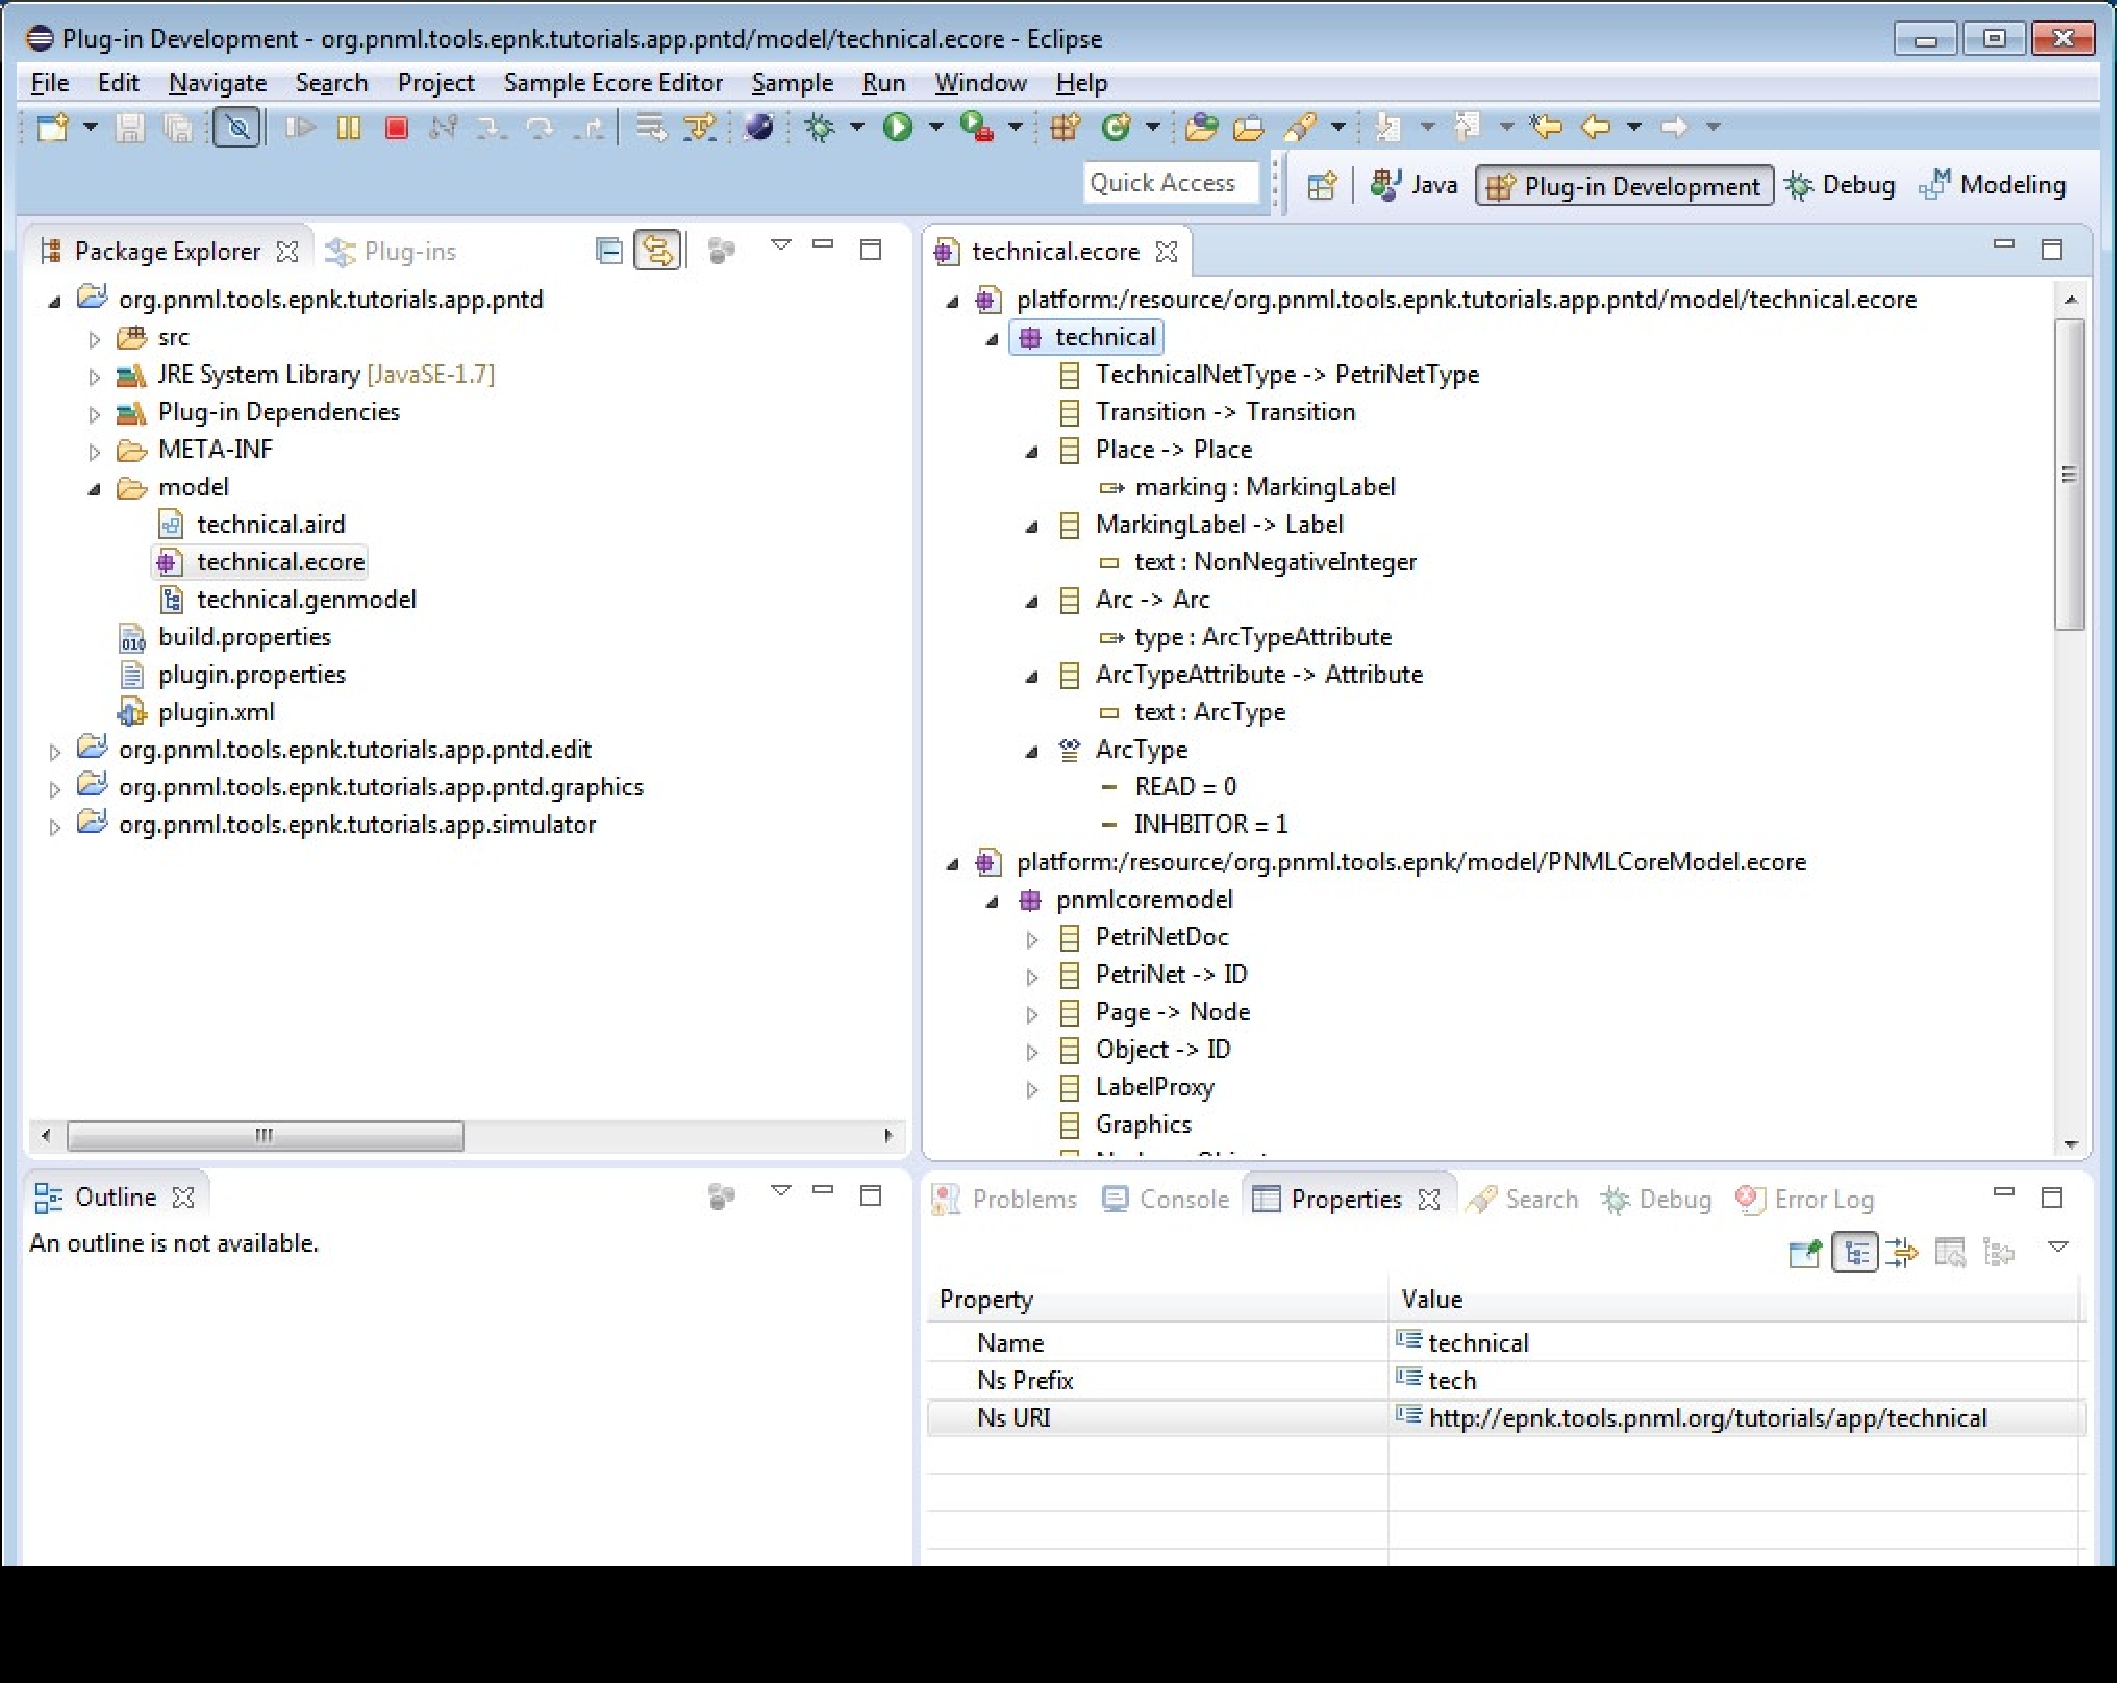
\includegraphics[scale=.34]{tutorial/ecore-tree-editor.pdf}}
  \centerline{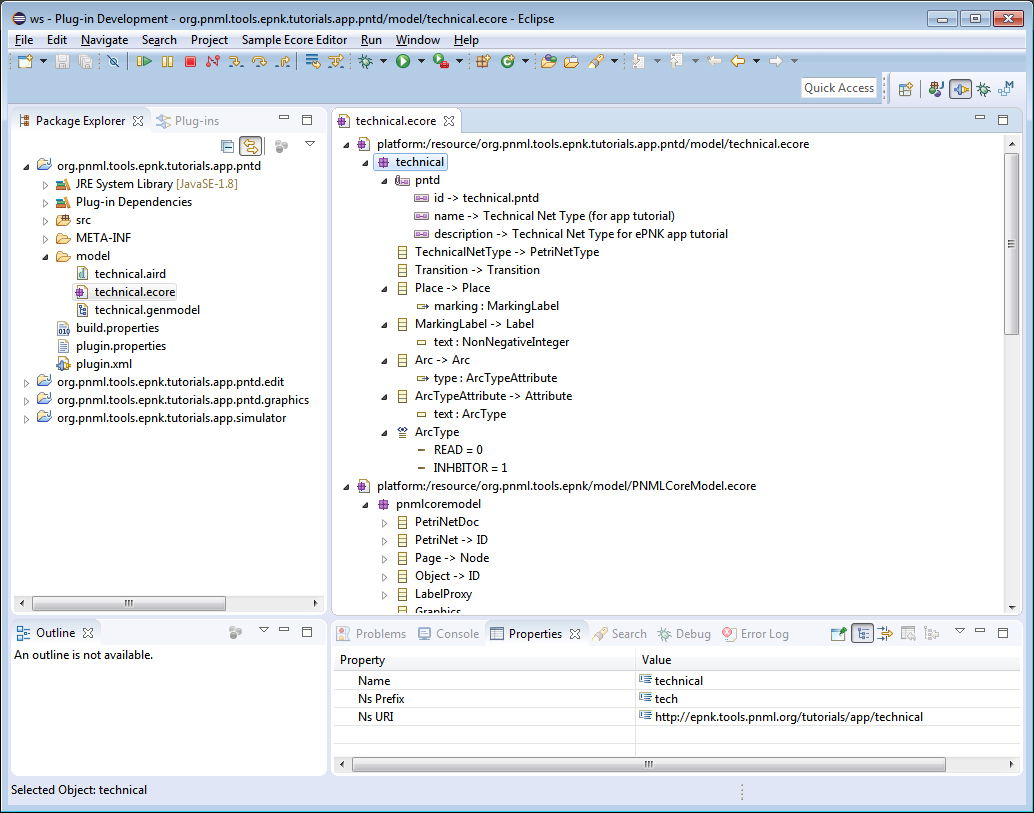
\includegraphics[scale=.34]{tutorial/ecore-tree-editor.jpg}}
  \caption{Ecore model of PNTD for technical net type in tree editor}
  \label{fig:tutorial:technical:pntd:ecore-tree}
\end{figure}

If you want, you can also open this model
in a graphical editor. To do this, you would need to switch to the ``Modeling''
perspective of your Eclipse workspace, and open the file {\tt technical.aird} by
double clicking on it; then navigate to ``Representation per category''
$\rightarrow$ ``Design'' $\rightarrow$ ``Entities'' $\rightarrow$ ``technical
class diagram'' and double click on $\rightarrow$ ``technical
class diagram''. Figure~\ref{fig:tutorial:technical:pntd:ecore-diagram} shows
the model when opened in the graphical editor.

\begin{figure}[hbtp!!]
  \centerline{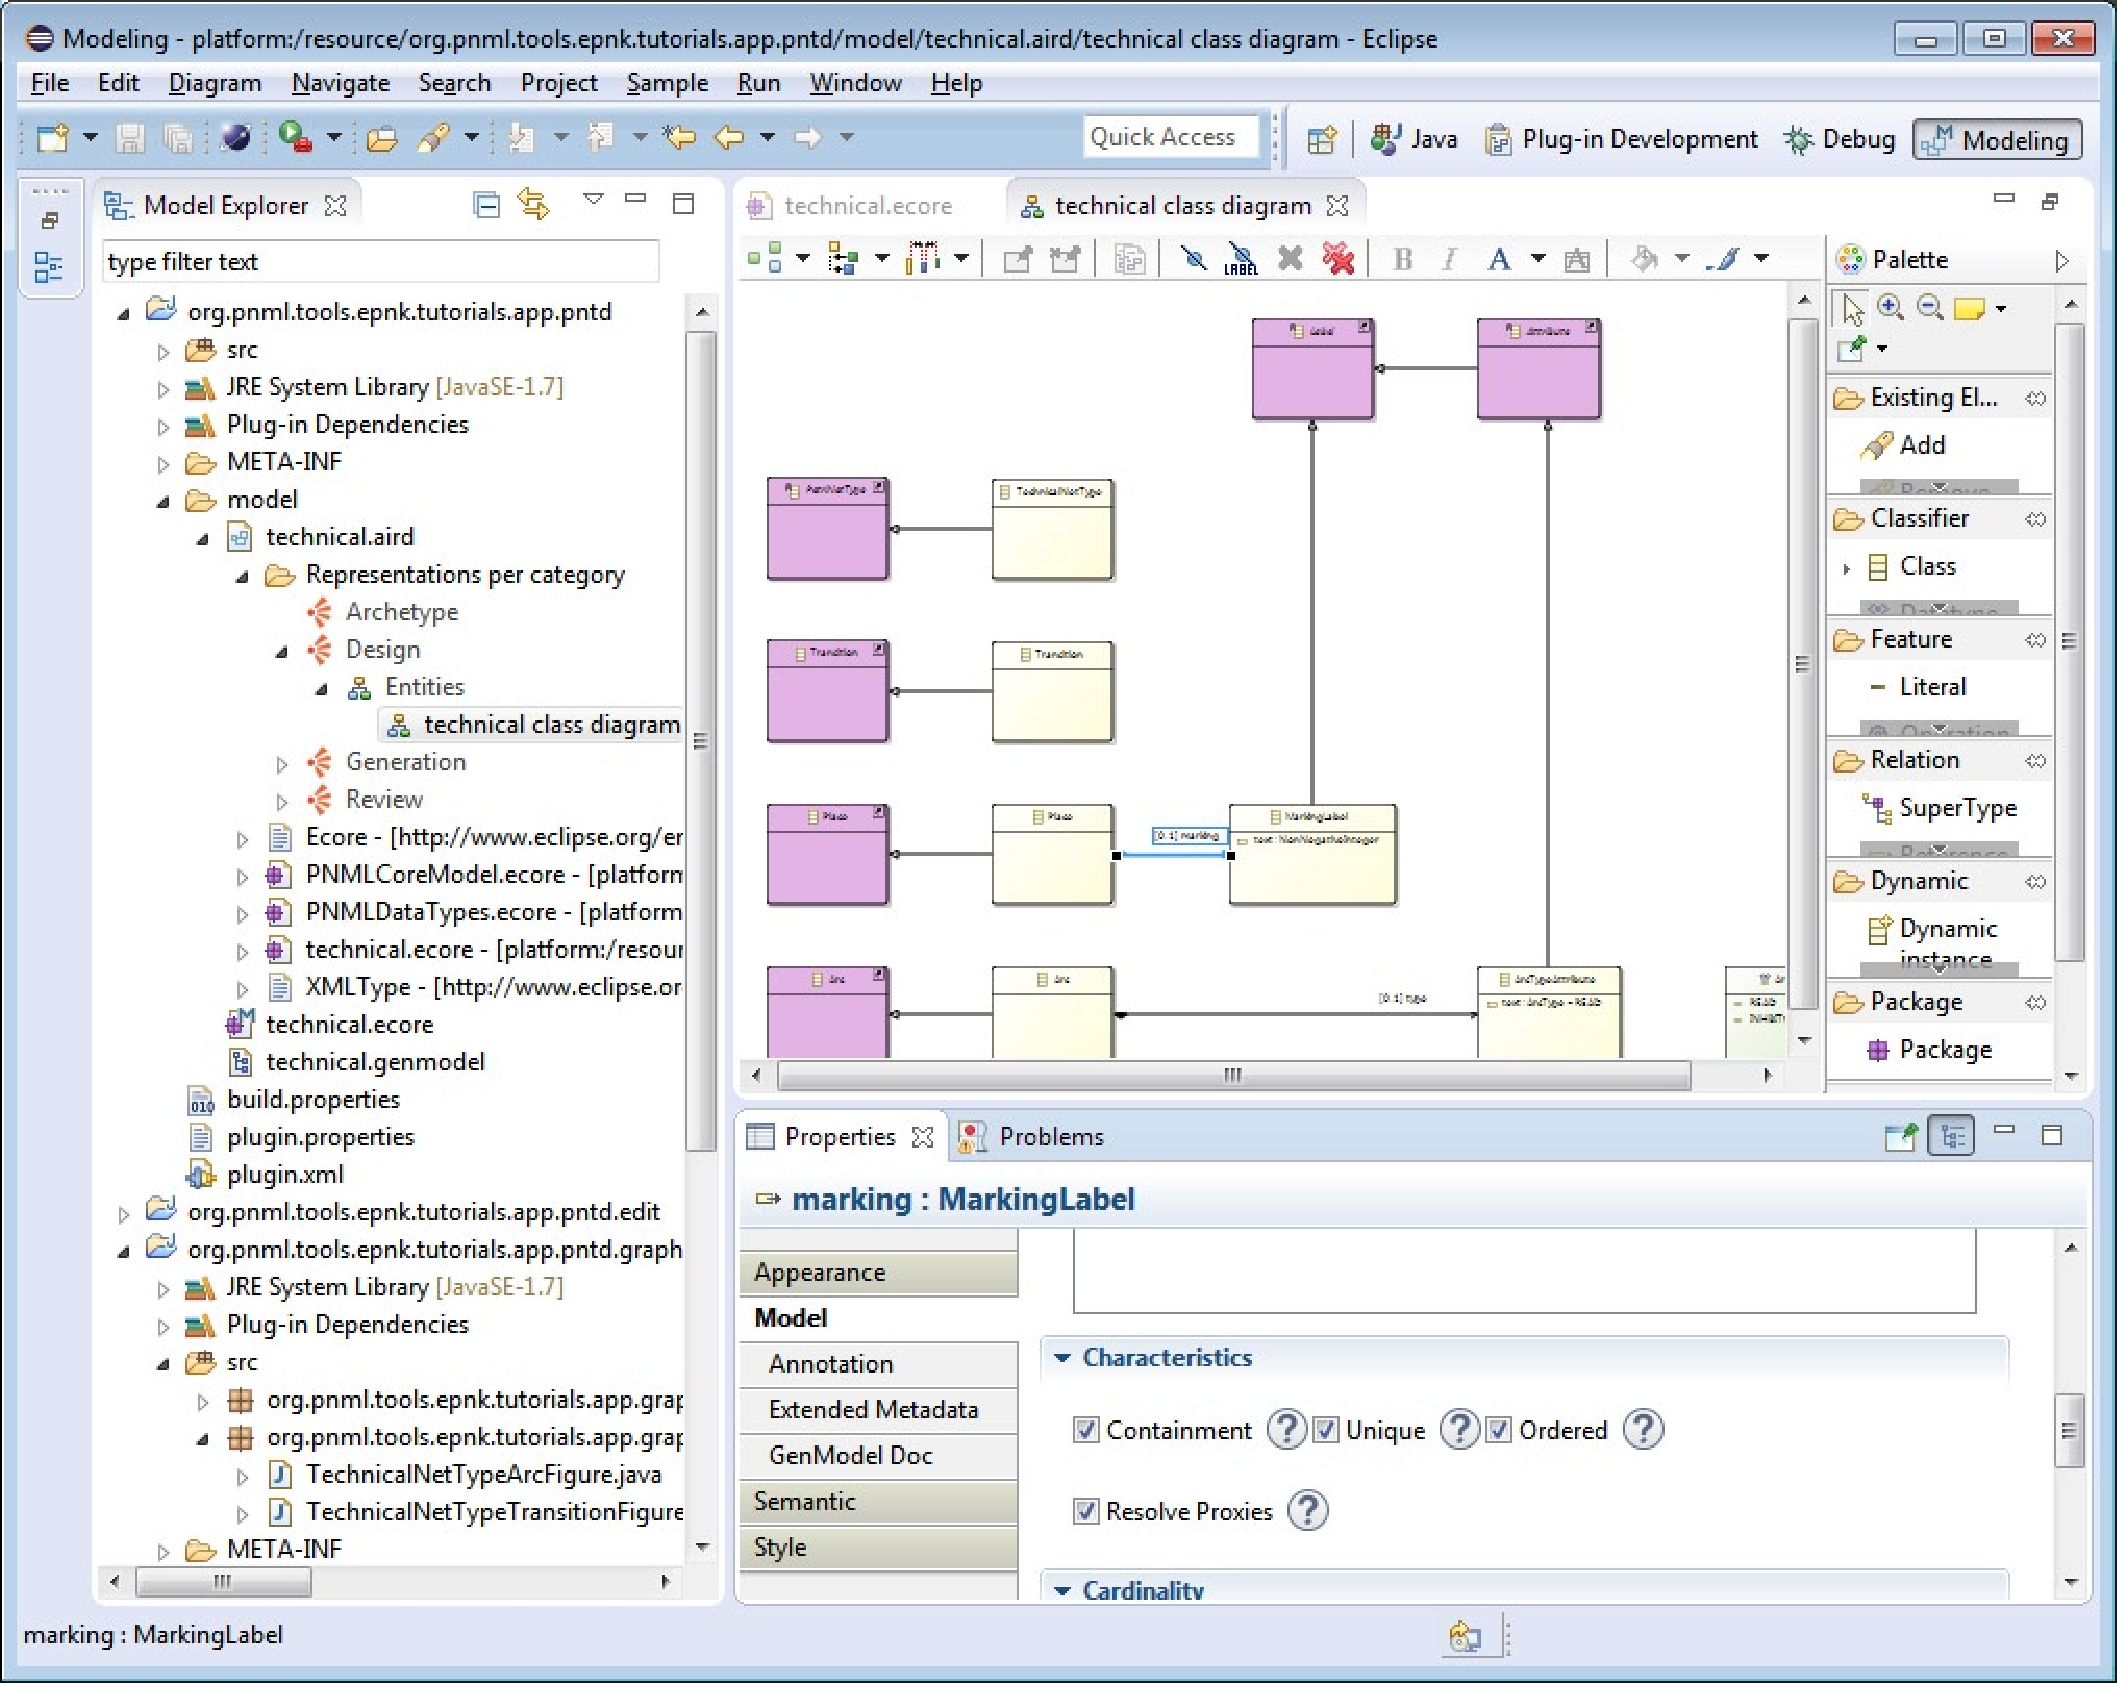
\includegraphics[scale=.34]{tutorial/ecore-diagram.pdf}}
  \caption{Ecore model for technical net type as diagram}
  \label{fig:tutorial:technical:pntd:ecore-diagram}
\end{figure}

We do not discuss the concepts of this model here again, since we
have discussed them already in Sect.~\ref{subsubsec:tutorial:concepts:pntd} in
Fig.~\ref{fig:tutorial:concepts:pntd}. 

\subsubsection{Creating the EMF project and model}
\label{subsec:tutorial:technical:pntd:ecore-creation}

Instead, we briefly discuss how to create such an EMF project and a model as
well as some technical details on how to edit some model features in this
subsection. Before you do this, it might be a good idea to switch back to
the ``Plug-in Development'' perspective in your Eclipse workspace.

A project which is based on a model from which code can be generated
automatically is called an \emph{EMF project}.  You can create a new empty
EMF project via the ``New'' action in the ``File'' menu of Eclipse. Select
``Other...'', and then, in the opened ``New'' dialog, select ``Empty EMF
project'' from category ``Eclipse Modeling Framework''.

In the newly created EMF project, you will find a folder {\tt model}, which is
where you should create a new Ecore model. A new Ecore model can be created
with the ``New'' action in the ``File'' menu. You will find the option ``Ecore
model'' in the ``Eclipse Modeling Framework'' category (try to use a
better name than ``My.ecore''); in the ``New'' dialog, you will be asked for
the top-level model object and the XML Encoding. The default should be
fine; make sure that the model object is set to {\tt EPackage}.

After you have created a new model, it will be shown in the Ecore tree
editor with a package with an empty name. Give a reasonable name to the package,
which uses non-capital letters, and choose a name space prefix and a unique URI
 representing your new package. The example from
Fig.~\ref{fig:tutorial:technical:pntd:ecore-tree} might give you an idea
on what to choose. Note however, that the domain
\url{http:\\epnk.tools.pnml.org} is reserved for the ePNK itself and for using
sub-domains of \url{tools.pnml.org} you would need to ask permission from
\url{http:\\www.pnml.org}.

In the newly created package, you should add one class which represents the
newly defined Petri net type. You can do that by right-clicking on the package
and then selecting ``New Child'' $\rightarrow$ ``EClass'' and give it a
reasonable name -- it is called {\tt TechnicalNetType} in our example. This
class must extend the class {\tt PetriNetType} from the {\tt pnmlcoremodel}. To this
end, you would need to set the class's ``ESuper Types'' in the properties view.
Before you can chose a class from the \emph{PNMLCoreModel}, you need to make
this package know to the editor. To do this, you need to load the resource containing
the {\tt pnmlcoremodel} in the tree editor. You can do this by right-clicking
somewhere in the tree editor and selecting ``Load Resource...''; then, in the
``Load Resource'' dialog, select ``Browse Target Platform Packages...'' and
select \url{http://org.pnml.tools/epnk/pnmlcoremodel}. Once you have done that,
you can select {\tt PetriNetType} as the ``ESuper Types'' in the properties view for your new class
for your Petri net type. Make sure to save this file right away.

Now you can continue adding the concepts of your new Petri net type. You should
add a class for each Petri net concepts that you want to extend and make sure
that it inherits from the corresponding class of the {\tt pnmlcoremodel}. The name
of these classes can, in principle, be any legal class name. But, you save a lot
of programming, if the class names are the same as in the  {\tt pnmlcoremodel} --
don't worry, since you have created them in a new package, there will be no
confusion with names, since your new classes live in a different name space. All new features
of your net type are represented by compositions to other classes, which need
to inherit from either {\tt Label} or {\tt Attribute} of the {\tt
pnmlcoremodel}. And these classes must have an attribute with name {\tt text}
and some data type. The data type can either be an existing data type, which
is built in to Ecore or defined in the ePNK, or a datatype defined in the new
package. In our example, the datatype {\tt ArcType} is an enumeration defined
in the package itself, the datatype  {\tt NonNegativeInteger} is defined by the
ePNK.

Note that in our example, the cardinality from the Petri net objects to its
features is $[0..1]$, which means that there can be zero or one of each feature
for every object of the respective type. But, the cardinality could also be $[0..*]$
allowing arbitrarily many instances of this feature for a single element. In the
tree editor for Ecore models, the value $-1$ as upper bound represents
``arbitrarily many''.

Note also that the reference from the Petri net object to its feature must
be compositions. In the Ecore model, this means that the property {\tt Containment}
of the respective reference must be set to {\tt true}.\\

At some point, it might be easier to edit and extend the Ecore model by using
a graphical editor. To this end, you can create a diagram for an existing Ecore
model: right-click on the file of the Ecore model and select ``Initialize Ecore
Diagram ...''; then, in the ``Create Representation File'' dialog, select a file
name and a folder for the diagram file (it should typically be in the same
folder as the model). In the ``Create Representation Wizard'', which opens after
a while, select ``Entities'' in category ``Design'' and continue; in the
next dialog select your package and give the diagram some name. In the diagram
editor that opens, double-click on ``here'' to create an initial representation
of you model. If you want to see related elements from other packages in this
diagram you can right-click on the diagram and select ``Add Related Elements''.
You will probably need to arrange the elements in a nicer way. In the end, don't
forget to save the diagram. Note that for opening the diagram again, you will
need to switch to the ``Modeling'' perspective of your Eclipse workspace as
discussed at the end of Sect.~\ref{subsec:tutorial:technical:pntd:ecore} for
Fig.~\ref{fig:tutorial:technical:pntd:ecore-diagram} already.

\subsubsection{Code generation}
\label{subsec:tutorial:technical:pntd:code-gen}

In order to plug in the PNTD defined by the Ecore model to the ePNK, we need to
first generate code from this model and make some adjustments to the code. The code will be generated
from a so-called \emph{gen model} that is associated with the Ecore mode and
defines some additional information for the code generator on how the code
should be generated and where the generated code should go.

In our example, the \emph{gen model} is the file {\tt technical.genmodel}. Once
opened in the \emph{EMF Generator} model editor, you can generate the code by
right-clicking on the top-level element and selecting ``Generate Model Code''
and ``Generated Edit Code''. You can also generate the other code, but you do
not need the ``Test Code'' and the ``Editor Code'' when using the model as
a PNTD for the ePNK.

When you have created a new EMF project and a new Ecore model, however, there
is no gen model yet. You first need to create the gen model for your new model
file.
You can do this by right-clicking on the file with the Ecore model and, then, selecting
``New'' $\rightarrow$ ``Other...'' and chosing ``EMF Generator Model'' from
category ``Eclipse Modeling Framework'' and following through the dialog. When
asked for the folder, make sure the gen model is in the same folder as the
model; when asked for the model URI, you will need to click on ``Load''\footnote
  {If clicking on load results in an error, there is probably some error in you
  Ecore model. Try to validate the Ecore model first and fix the error.}
and continue. At some point, a dialog for selecting the packages for which the
gen model should be generated will show up, which looks like the one
shown in Fig.~\ref{fig:tutorial:technical:pntd:gen-model-select-package1}.
Note that it crucial, that in this dialog you only select your package as
``Root package''; all the other ones, you should select in ``Referenced
generator models''. Before you continue, your selection in this dialog
should look like shown in
Fig.~\ref{fig:tutorial:technical:pntd:gen-model-select-package2}. Once you made
these selections, you can ``Finish'' the generation of the gen model.

\begin{figure}[hbtp!!]
  \centerline{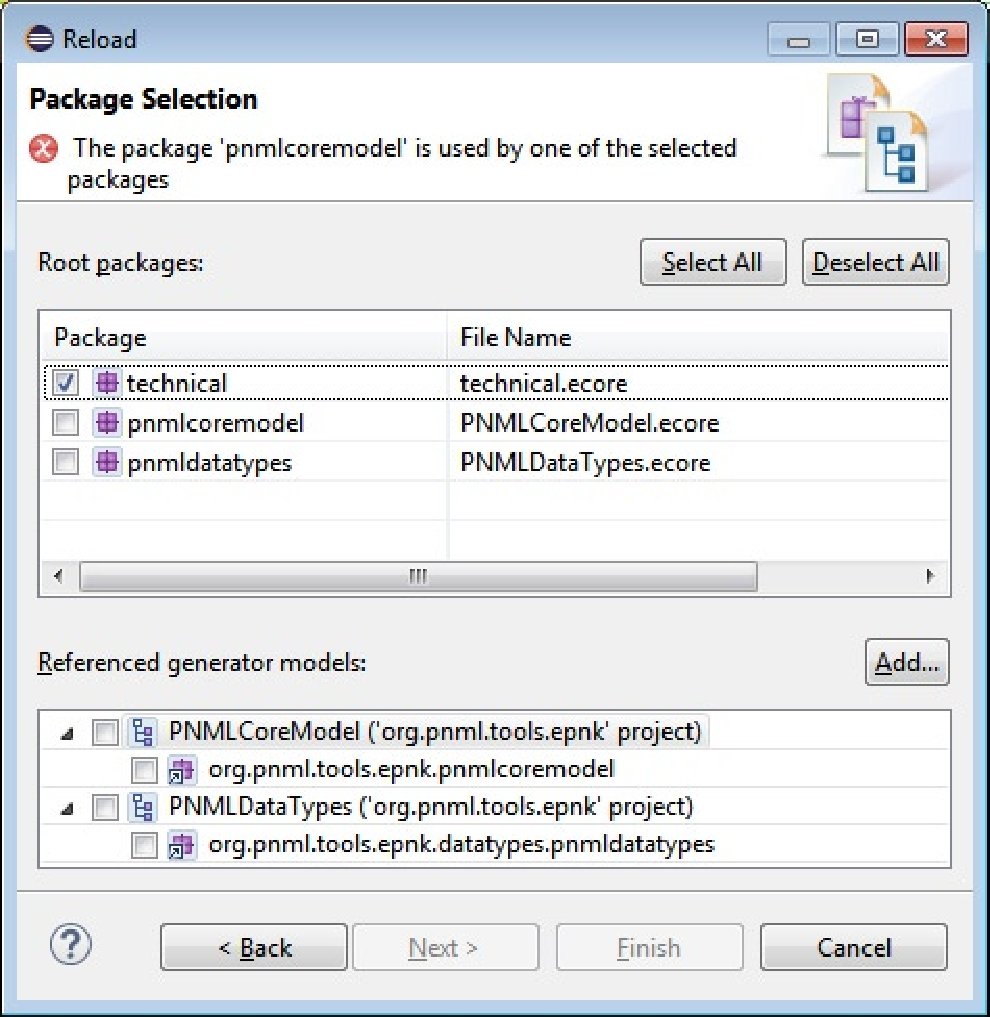
\includegraphics[scale=.48]{tutorial/PackageSelection.pdf}}
  \caption{Select Package Dialog}
  \label{fig:tutorial:technical:pntd:gen-model-select-package1}
\end{figure}

\begin{figure}[hbtp!!]
  \centerline{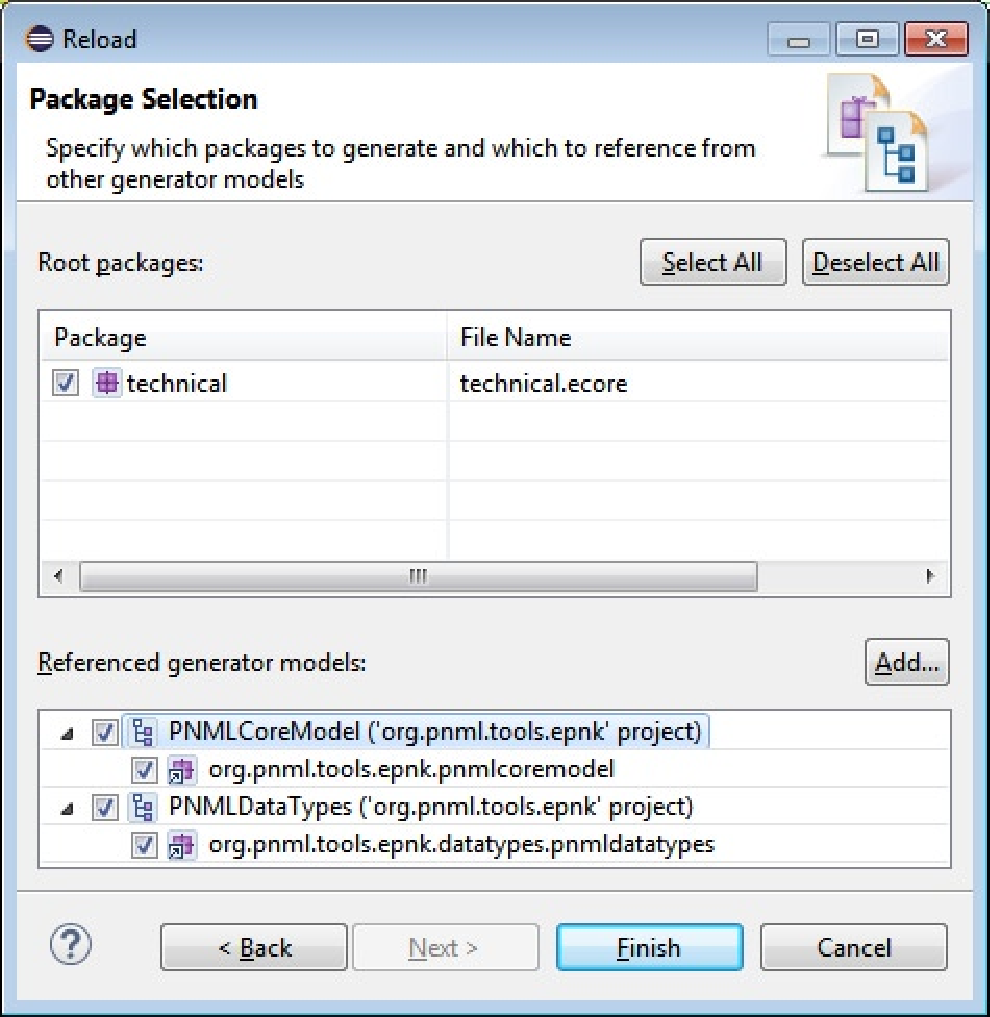
\includegraphics[scale=.48]{tutorial/PackageSelection2.pdf}}
  \caption{Select Package Dialog}
  \label{fig:tutorial:technical:pntd:gen-model-select-package2}
\end{figure}

Then the gen model for your model file should be created, and it should be open
in the ``Gen Model'' editor. Before you generate code from this new gen model,
you need to make two manual changes in this gen model. First, select the
top-most element and change one property in the properties view: change the property
{\tt Operation Reflection} in the category {\tt Model} to {\tt false}. Second,
open the top-level element and select the package element. For this package,
set the property {\tt Base Package} to some reasonable Java package name;
in our example, it is set to
{\tt org\qnsep{}pnml\qnsep{}tools\qnsep{}epnk\qnsep{}tutorials\qnsep{}app};
this setting directs the generator to generate the code in a
subpackage of this Java package.

Now, you can generate the model and the edit code from this gen model as
discussed above. The generated code should show no errors; if it does, you
probably forgot to change the property {\tt Operation Reflection} to {\tt
false} in the gen model after generating it.

Note that, if you should make changes in the model later on, you would need
to ``Reload'' your gen model again, so that it can become aware of the model
changes and update accordingly (reusing as much as possible from the existing
settings). In order to do that, first make sure that you have saved and closed
your model file. Then, right-click on the gen model and select ``Reload'' and
follow through the dialog which very much works like the dialog for
initially creating the gen model.

\subsubsection{Manual changes in the code}
\label{subsec:tutorial:technical:pntd:code-manual}

Before plugging in the generated net class to the ePNK, we need to make
two manual changes in the Java class generated for the class {\tt
TechnicalNetType}, which represents the new Petri net type defined in this
tutorial. In our example, this class can be found in the {\tt src} folder in
package {\tt
org\qnsep{}pnml\qnsep{}tools\qnsep{}epnk\qnsep{}tutorials\qnsep{}app\qnsep{}technical\qnsep{}impl}
and is called {\tt TechnicalNetType\optsep{}Impl}.

The two changes that need to be made in this class are the following: first,
the constructor of this class must be made public, which is necessary so that
the ePNK will be able to create new instances of this class. Second, the
{\tt toString()} method of this class must be implemented; it should return a
URI, which uniquely identifies Petri nets of this type in PNML. It must be
a string representing a URI. In principle, it can be any URI, you just need to
make sure that it is unique.

\begin{figure}[htbp!]
% \lstinputlisting[label=lst:tutorial:technical:pntd:code-manual,language=Java,tabsize=2,stringstyle=\small,%
\lstinputlisting[label=lst:tutorial:technical:pntd:code-manual,tabsize=2,stringstyle=\small,%
caption={Manual changes in class {\tt TechnicalNetTypeImpl}}]%
  {code/tutorial/TechnicalNetType-java.txt}
\end{figure}

Listing~\ref{lst:tutorial:technical:pntd:code-manual} shows the class
{\tt TechnicalNetTypeImpl}  with the changes made in lines 15--19 and 26--37,
highlighted in red. Note that for readability reasons, we have omitted some
comments, but otherwise the class is completely shown. In addition to
making the constructor public and implementing the {\tt toString()} method,
the changes are marked with the tag {\tt \@generated NOT}, which indicates
that there are manual changes to the generated code, and this way prevents the
manual changes being overwritten the next time the code is generated again
from the gen model.\\

The above changes are the only code that needs to be written manually for making
the new Petri net type work with the ePNK. In our example, we have three
additional Java classes, which are written completely manually. One implements
a Java constraint, which is discussed in
Sect.~\ref{subsec:tutorial:technical:constraints}. The other two are convenience
classes, which make it easier to implement our simulator and constraints later.
Since it is good practice and increases maintainability to have such convenience
classes with static methods, we briefly discuss them here, even though we do not
need them right away.

\begin{figure}[htbp!]
\lstinputlisting[label=lst:tutorial:technical:pntd:code-type,language=OCL,tabsize=2,stringstyle=\small,%
caption={Enumeration with all {\tt ArcType}s}]%
  {code/tutorial/ArcType-java.txt}
\end{figure}

In Listing~\ref{lst:tutorial:technical:pntd:code-type}, you can see a Java
enumeration for arc types. Remember, that our model of the PNTD has a similar
type; but in the model, there have been two possible values only: {\tt READ} and
{\tt INHIBITOR}. The end-user will only be able to set the type attribute
of arcs to these two values -- and the value can be left undefined. In
Listing~\ref{lst:tutorial:technical:pntd:code-type}, the enumeration defines
the values of all possible \emph{interpretations} of arc types. The static
method {\tt getArcType()} shown in Listing~\ref{lst:tutorial:technical:pntd:code-helper}
shows, how to compute the ``interpretation'' from the actual value set for
the arc and its source and target nodes it is connected to. It is crucial to
implement such an ``interpretation'' only once in the manually written code;
otherwise this code would be repeated and scattered all over the project
-- possibly even using different interpretations in different parts of the
software -- making maintenance a nightmare.

\begin{figure}[htbp!]
\lstinputlisting[label=lst:tutorial:technical:pntd:code-helper,language=OCL,tabsize=2,stringstyle=\small,%
caption={Class {\tt TechnicalNetTypeFunctions} with static helper methods}]%
  {code/tutorial/TechnicalNetTypeFunctions-java.txt}
\end{figure}

Note that the code from Listing~\ref{lst:tutorial:technical:pntd:code-type}
and~\ref{lst:tutorial:technical:pntd:code-helper} is written completely
manually, and does not run the risk of being overwritten by the code generator. Since the
code is part of an EMF project, where most code is automatically generated,
the code is tagged with {\tt \@generated NOT} anyway. This makes it
easy to search for all code which is not generated. In the project for the
PNTD, there are actually five manual changes: two of them in the class for the
net type and three manually written classes (the third class is discussed
later in Sect.~\ref{subsec:tutorial:technical:constraints}).

Since we might want to use the class {\tt TechnicalNetTypeFunctions} in our
other projects later, we need to export the Java package containing it
from this project. You can do that by using the ``Plug-in
manifest'' editor by double-clicking on the {\tt plugin.xml} and selecting
the ``Runtime'' tab. In that tab, you should add the respective Java package to
``Exported Packages'' by pressing the ``Add...'' button.

\subsubsection{Plugging in the PNTD}
\label{subsec:tutorial:technical:pntd:plugin}

The last step of defining a PNTD for the ePNK is actually plugging the generated
and manually changed class for the net type, {\tt TechnicalNetTypeImpl} in our
example, in to the ePNK. This could be done by using the Eclipse ``Plug-in
manifest'' editor. But, it is actually easier to do that directly by changing
the XML code of the {\tt plugin.xml}. To this end, open the {\tt plugin.xml}
file with the `Plug-in manifest'' editor by double-clicking on it and go to
the tab called ``plugin.xml''.

Listing~\ref{lst:tutorial:technical:pntd:plugin-xml} shows the snipped from the
{\tt plugin.xml}, which plugs the PNTD in to the ePNK. It is a usual Eclipse
\emph{extension}  referring to the \emph{extension point} {\tt
org.pnml.tools.epnk.pntd} (line~4), which is defined by the ePNK. The attributes
{\tt id} and {\tt name} is just a unique id and name for this new Petri net
type. The actual new type is defined in the {\tt type} element in lines 5--7;
its attribute {\tt class} refers to our class {\tt TechnicalNetTypeImpl},
which we had modified manually earlier and which defines the new Petri net type.
We need to refer to this class by its fully qualified Java class name
(including the packages); the description is just some text describing the new Petri net type.
 
\begin{figure}[htbp!]
\lstinputlisting[label=lst:tutorial:technical:pntd:plugin-xml,language=OCL,tabsize=2,stringstyle=\small,%
caption={{\tt plugin.xml} snipped plugging the PNTD in to the ePNK}]%
  {code/tutorial/plugin-xml-pntd.txt}
\end{figure}

Note that at this point, with only the project {\tt
org\qnsep{}pnml\qnsep{}tools\qnsep{}epnk\qnsep{}tutorials\qnsep{}app\qnsep{}pntd}
and the automatically generated project
{\tt org\qnsep{}pnml\qnsep{}tools\qnsep{}epnk\qnsep{}tutorials\qnsep{}app\qnsep{}pntd\qnsep{}edit},
we can use our Technical Petri
net type with the ePNK already. The only problem would be that \emph{read},
\emph{inhibitor} and \emph{reset} arcs would not be shown with a dedicated
graphics. All arcs would be graphically shown as \emph{normal} arcs. Moreover,
the end-user would still be able to draw arcs between arbitrary nodes, even
between pages. We discuss how to fix the latter problem in the next section, and
how to fix the first problem in Sect.~\ref{sec:tutorial:technical:graphics}.

Whenever you create a new Petri net type, it would be a good idea to check
whether your PNTD works with the ePNK at this point. Only after that, you should
proceed.

\subsection{Constraints}
\label{subsec:tutorial:technical:constraints}

In this section, we discuss how to define and plugin constraints for a
net type, so that the ePNK (and Eclipse in general) will take them into account.

As discussed in Sect.~\ref{subsubsec:tutorial:concepts:pntd}, we have two
constraints for our \emph{technical Petri net type}. The first is that an
arc should run from a place to a transition or the other way round, or it
should run from a page to a transition; moreover, only an arc running from 
a place to a transition can have a type (for the other arcs, the type attribute
should not be set). In Listing~\ref{lst:tutorial:concepts:pntd:ocl}, we have
already seen an OCL formulation of that constraint. The other constraint was
that there should be no duplicate read or inhibitor arcs between a place and
a transition. This constraint is realized as a Java constraint.

All constraints are defined in the our PNTD project {\tt
org\qnsep{}pnml\qnsep{}tools\qnsep{}epnk\qnsep{}tutorials\qnsep{}app\qnsep{}pntd},
which defined the PNTD. The reason
is that constraints conceptually are a part of a model. Actually, it would
be possible to include the constraints to the Ecore model. But, we follow
a slightly here.

\subsubsection{OCL constraint}
\label{subsubsec:tutorial:technical:constraints:ocl}

We start with discussing how to add the OCL constraint for properly connecting
arcs to the project. This can be done by pluging in an OCL constraint by
defining it in the {\tt plugin.xml} of the project
{\tt org\qnsep{}pnml\qnsep{}tools\qnsep{}epnk\qnsep{}tutorials\qnsep{}app\qnsep{}pntd}.
Listing~\ref{lst:tutorial:technical:constraint:ocl} shows the part of
{\tt plugin.xml} that defines a constraint provider, with the OCL
constrain for arcs. All of that snippet is necessary, but we highlight
some more important settings and features in the definition (marked in red).

The most important part is the actual OCL constraint, which we had shown
in Listing~\ref{lst:tutorial:concepts:pntd:ocl} on
page~\pageref{lst:tutorial:concepts:pntd:ocl} already. The OCL constraint
Listing~\ref{lst:tutorial:technical:constraint:ocl}
is shown as XML CDATA in order to escape all the special symbols of OCL in lines
30-39. Note, however that the first line from
Listing~\ref{lst:tutorial:concepts:pntd:ocl}, which gave the context is missing here.
This context is actually defined by the target element in lines 21--28:
the {\tt class} attribute defines the Ecore class it refers to by the name
{\tt Arc} of the class followed by the package URI of the model package in which
it is defined. The target also defines \emph{events} which cause the validator to check the
constraint again. In our example, these are set events of the features {\tt
source}, {\tt target} and {\tt type} of the arcs; this means that the validator
kicks is whenever one of these features is of an arc changes. This goes
together with the fact that we define the constraint as a \emph{live constraint}
(see line 10), which means that after any change an end-user makes (with respect
to the defined events), the constraint is checked. If the constraint should fail, the complete
action of the end-user will be undone. Therefore, the end-user cannot create
a model that is invalid with respect to a \emph{live constraint}, provided that
the event definition covers all features and events that might invalidate a
constraint of an arc. In our case, these features are {\tt source}, {\tt target}
and {\tt type}.

\begin{figure}[htbp!]
\lstinputlisting[label=lst:tutorial:technical:constraint:ocl,tabsize=2,stringstyle=\small,%
caption={{\tt plugin.xml} defining the OCL constraint for arcs}]%
  {code/tutorial/plugin-xml-ocl.txt}
\end{figure}

In addition, there is a \emph{severity} of the constraint (line~12), which is an
\emph{error} in our example, and \emph{language} of the constraint (line~9) is
defined as OCL. Moreover, there is a message, which will be output to the
end-user, whenever the validation fails -- and the message of the problem marker
attached to the model element.
The tag $\{0\}$ in this message, will be replaced with the object on which the
constraint failed (the \emph{target}).

Actually within the same constraint provider, more than one constraint can be
defined, which is indicated by the $\ldots$ in line~42. We will actually see an
additional constraint there when discussing the Java constraint in the following
section.\\

\begin{figure}[p!!]
  \centerline{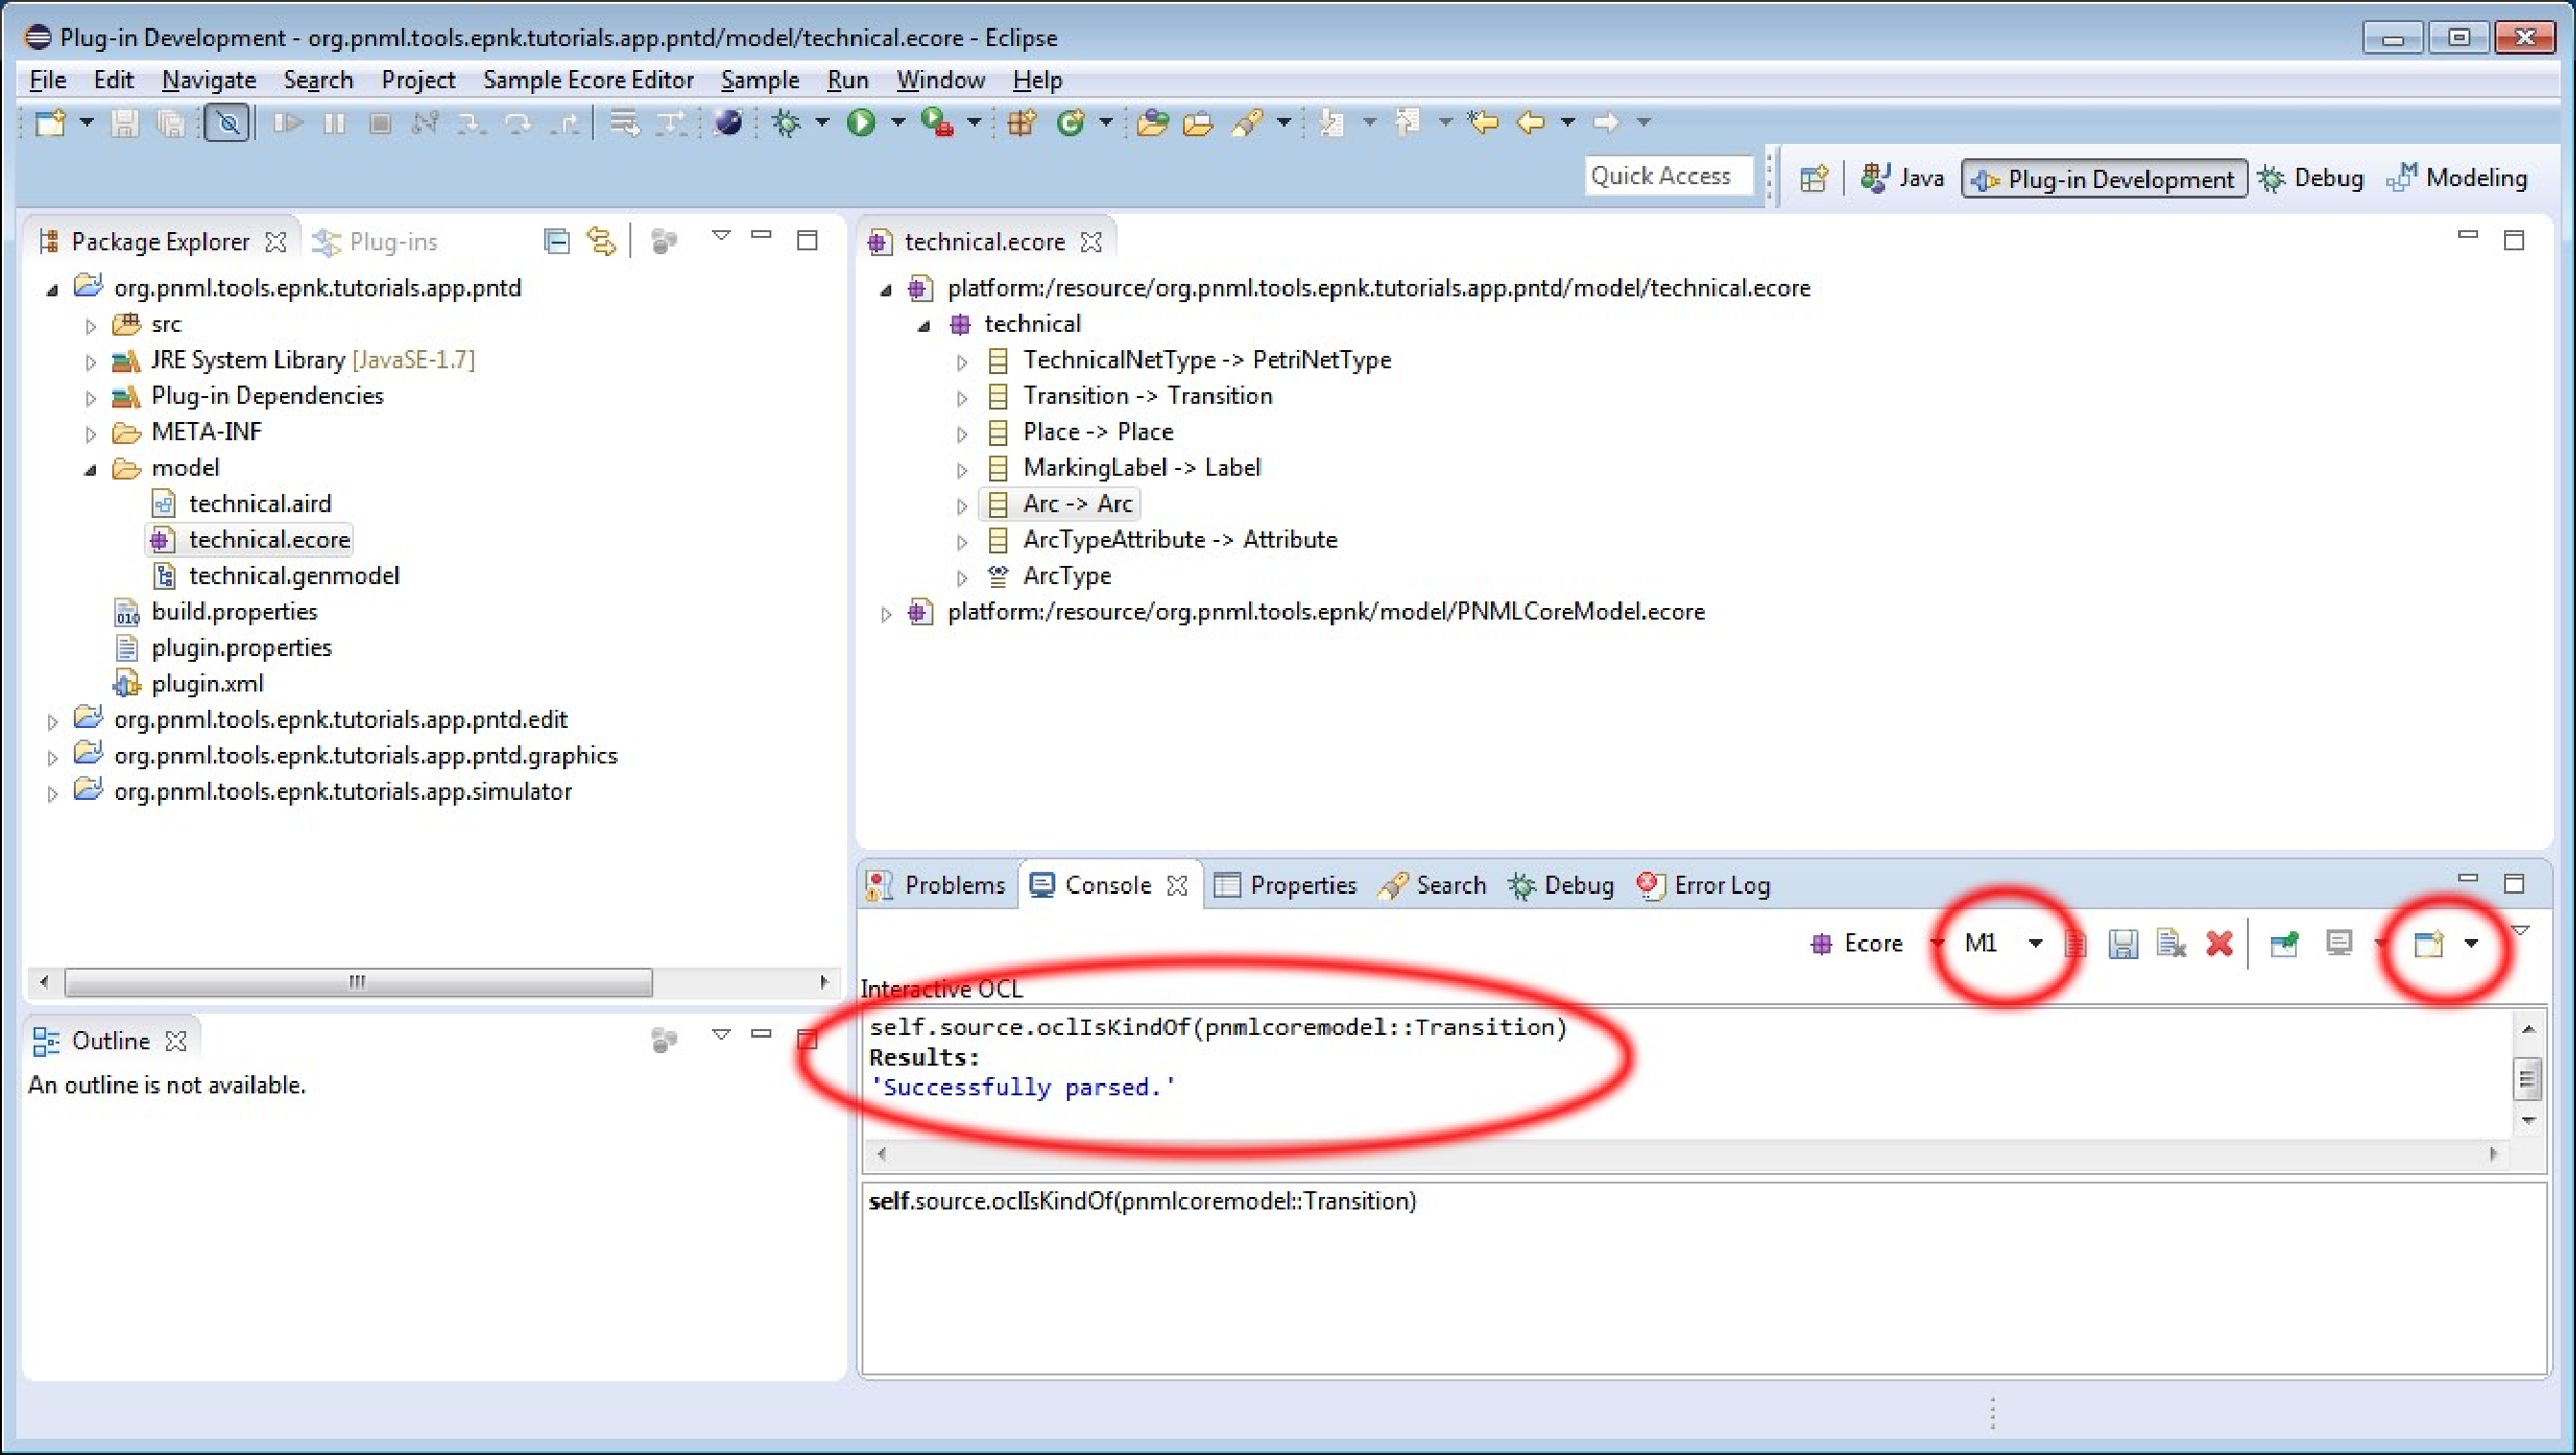
\includegraphics[scale=.27]{tutorial/ocl-console-m1.pdf}}
  \caption{OCL console in Eclipse development workbench}
  \label{fig:tutorial:technical:constraints:ocl:m1}
\end{figure}

Note that the OCL constraint must be syntactically correct, and getting the
syntax of OCL right might be a bit tricky if you do not have much experience.
Experimenting with the OCL syntax by changing the OCL constraint in the
{\tt plugin.xml}, starting the runtime workbench and testing whether the OCL
constraint works, and staring all over again, if it does not work, is way too
time consuming. We need a more efficient way to get the OCL syntax right --
and even a way to check how an OCL expression evaluates in a given situation.
To this end, we had recommended to install the ``OCL Examples
and Editors SDK'' feature to your Eclipse in
Sect.~\ref{sec:tutorial:technical:install:eclipse}. If this feature is installed
in Eclipse, you can open the ``Console'' view, and in that view select
``Interactive OCL'' as shown in
Figure~\ref{fig:tutorial:technical:constraints:ocl:m1}. In this console, select
M1 in the drop down menu (marked by a red circle). If you then select an element
in the Ecore editor, you can type some OCL constraint in the field at the bottom of the ``Interactive
OCL'' view and check whether it is syntactically correct (you even get some
syntax support, which indicates possible options while typing).
Once you type enter, the field on top will show whether the syntax of the OCL
constraint for the element selected in the Ecore model is syntactically correct.

Actually, the ``Interactive OCL'' console can not only be used for checking the
syntactical correctness of OCL constraints. If you start the runtime workbench,
and open an instance of a model, you can select an element of the instance, and
evaluate an OCL expression on this instance. For example, you could open a
PNML document and a page in the graphical editor, select an arc and evaluate the
constraint. This is shown in
Fig.~\ref{fig:tutorial:technical:constraints:ocl:m2}, where the OCL expression
{\tt self.type.text} is evaluated on an arc (the one running from place $p_7$
to transition $t_5$; the evaluation shows that it is an inhibitor arc. Note that
you need to switch the ``Interactive OCL'' console to ``Modeling level'' M2 for
this purpose.

\begin{figure}[p!!]
  \centerline{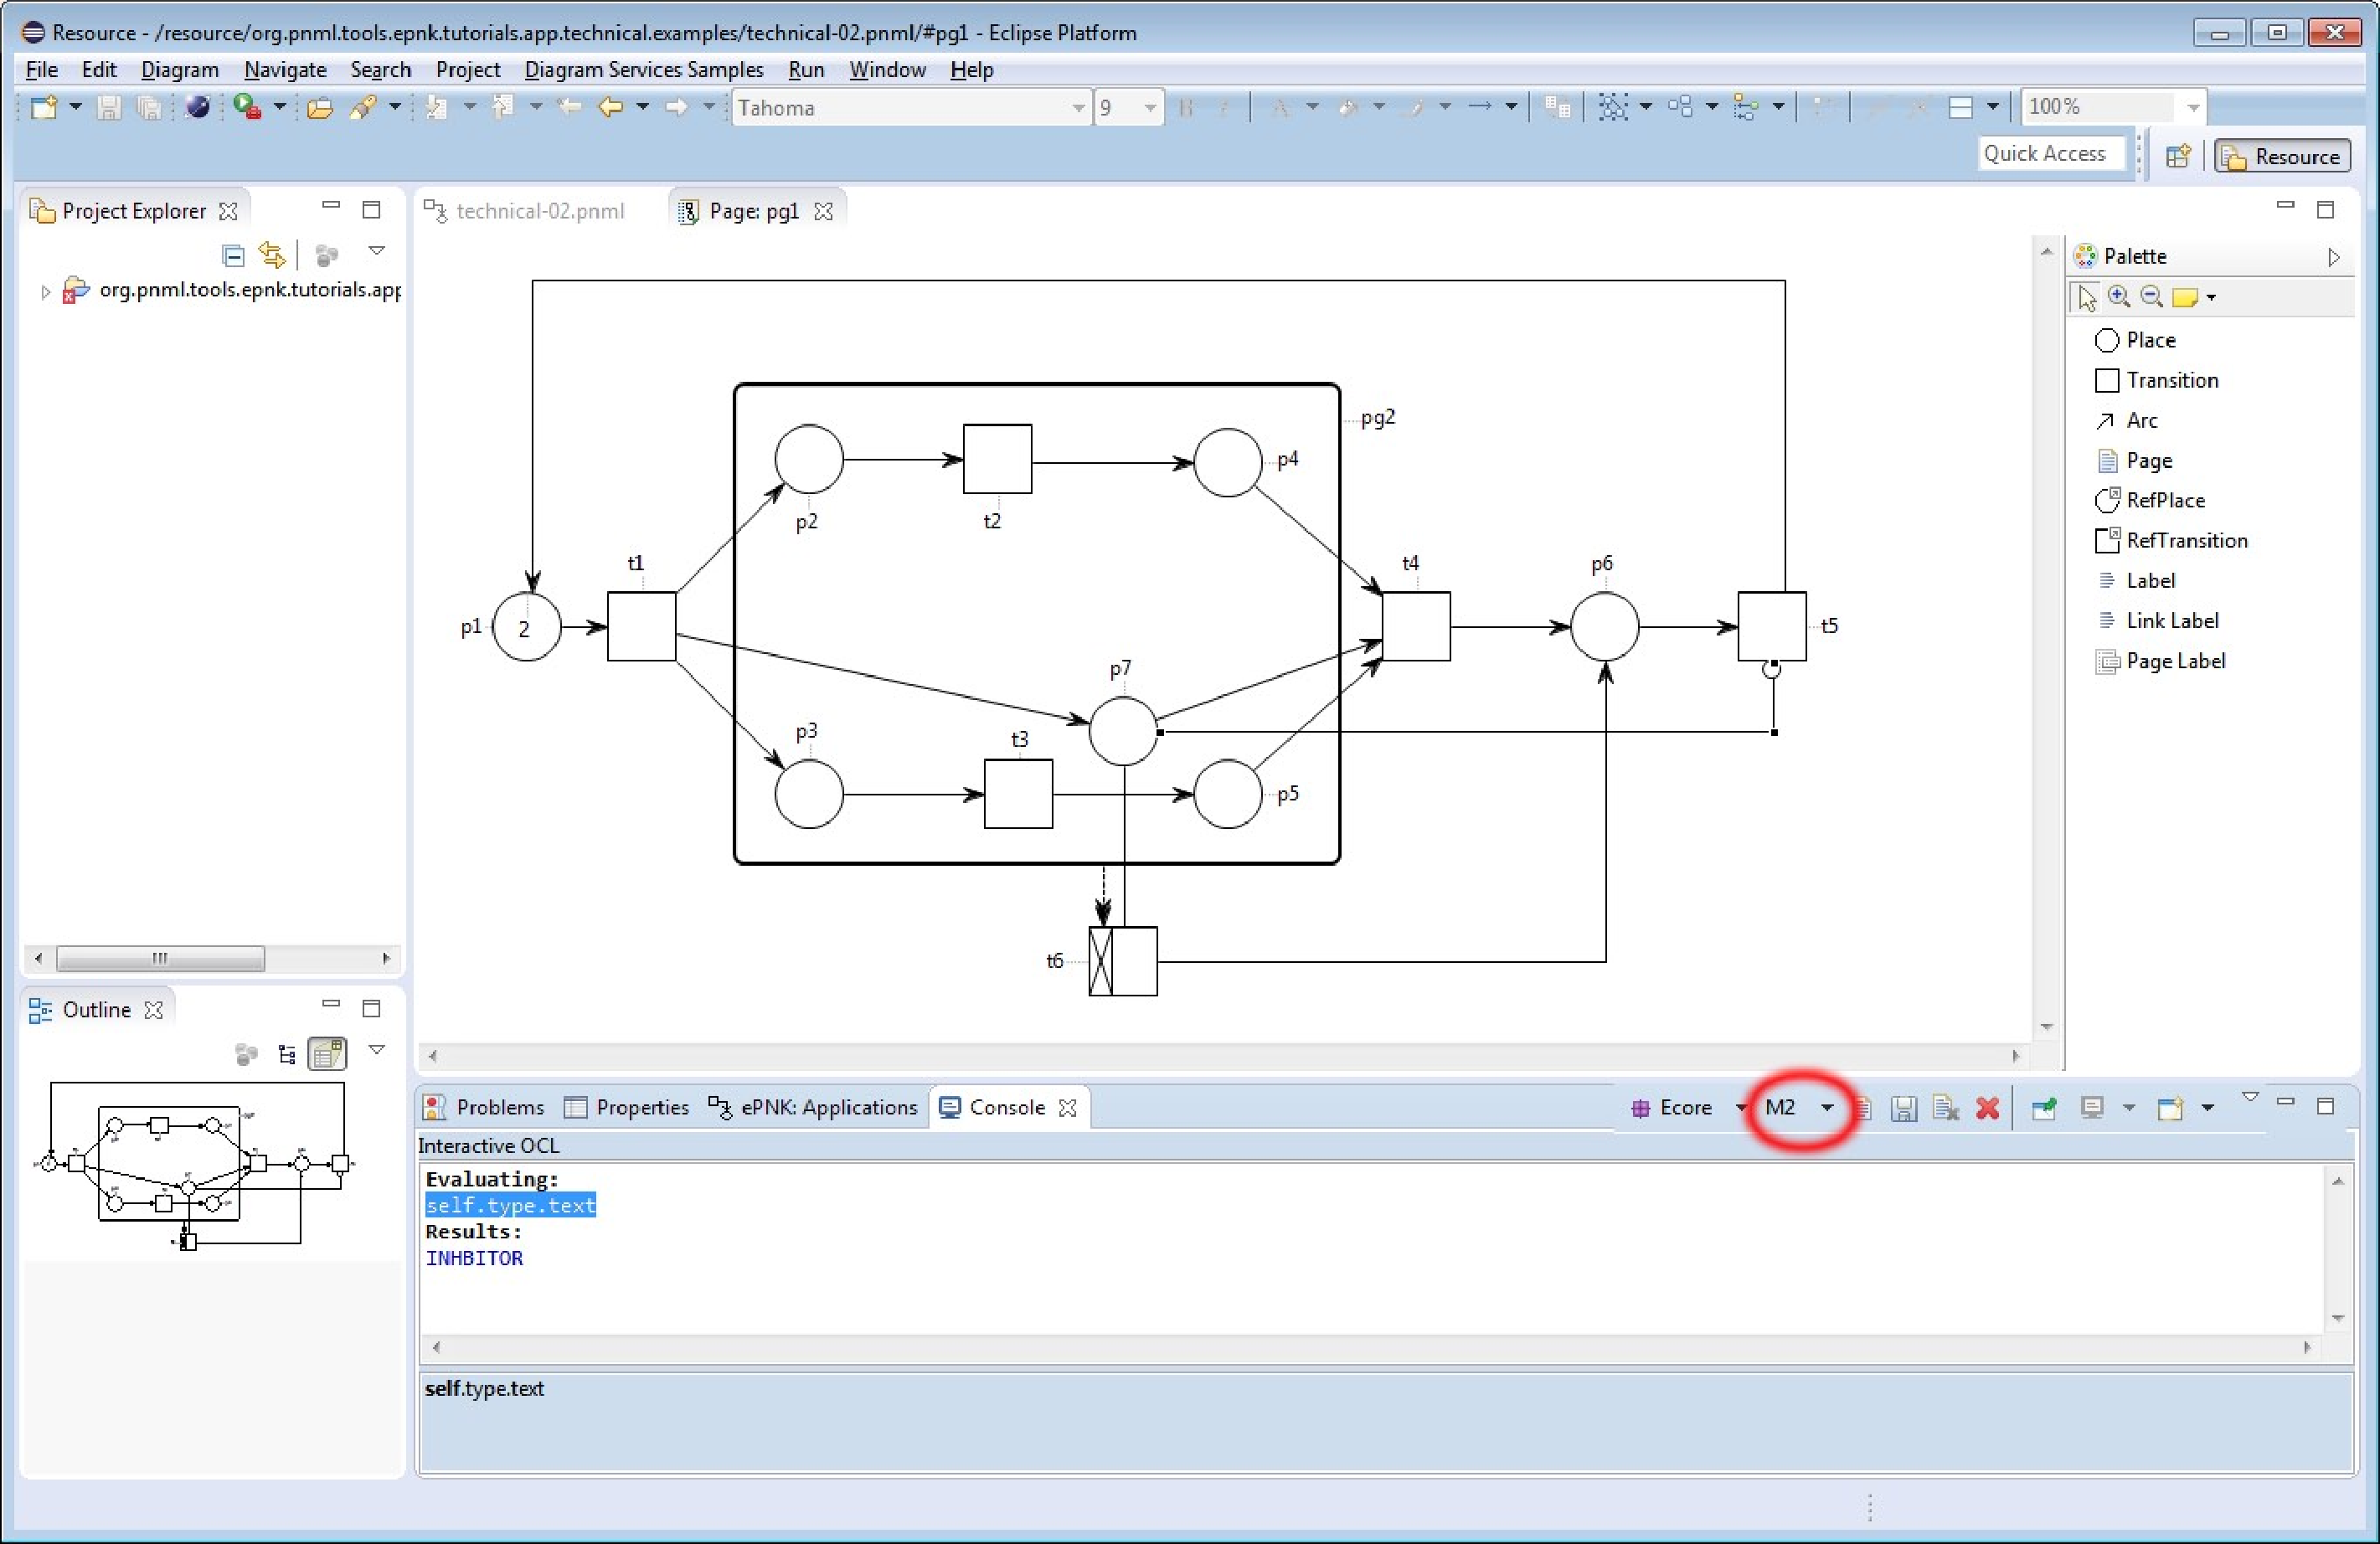
\includegraphics[scale=.27]{tutorial/ocl-console-m2.pdf}}
  \caption{OCL console in Eclipse runtime workbench}
  \label{fig:tutorial:technical:constraints:ocl:m2}
\end{figure}

Checking syntactical correctness, exploring the possible options for
expressions, and even for checking whether an OCL expression is evaluating as
expected, the ``Interactive OCL'' console is a very efficient tool.

\subsubsection{Java constraint}
\label{subsubsec:tutorial:technical:constraints:java}

Listing~\ref{lst:tutorial:technical:constraint:java} shows a Java implementation
of a constraint, which guarantees that there are no duplicate arcs of type
\emph{read} or \emph{inhibitor} between the same nodes. The {\tt validation()}
method of this class is called with some validation context from which the object on which the constraint
should be checked can be obtained (the \emph{target} that will be defined when
the constraint is plugged in). 

The implementation of the {\tt validation()} method first obtains the target
object form the validation context and checks whether it is an {\tt Arc} of
the our technical arc type. Then, it computes the ``interpreted'' type,
of the arc via the utility class {\tt TechnicalNetTypeFunctions}, which
we had discussed in Sect.~\ref{subsec:tutorial:technical:pntd:code-manual},
as well as the nodes to which the source and target of this arc resolve (in
case these are reference nodes); this is done with the {\tt NetFunctions}
utility class coming from the ePNK.

After that a so-called {\tt FlatAccess} object is obtained, which allows us to
obtain all arcs that conceptually belong to a node, even when the node is actually
split up via reference nodes on different pages. In case the arc is an
\emph{inhibitor} or \emph{read} arc, and it has a source node and if the
flatAccess object could be obtained, it iterates over all the other arcs that
have the source node as their source too. The set of all these arcs can be
easily obtained from the {\tt flatAccess} object. Than it checks for all
these {\tt other} arcs (if they are different from the arc itself), whether
the  {\tt other} arc is a duplicate, i.e.\ whether the other arc has the same
target and the same type. In that case, the {\tt validation()} method returns
a failure status using the context -- the singleton array contains the arc
on which the constraint had failed.

\begin{figure}[htbp!]
\lstinputlisting[label=lst:tutorial:technical:constraint:java,tabsize=2,stringstyle=\small,%
caption={Java class implementing the no duplicate arcs constraint}]%
  {code/tutorial/NoDuplicateArc-java.txt}
\end{figure}

Basically, a Java constraint is a class implementing a {\tt validation()}
method, which should return a failure status when the constraint is violated
on the target object and a success status otherwise. The rest is left to your
Java skills -- which, it in many cases, makes Java constraints easier to
formulate than OCL even tough the implementation looks a bit more verbose.

Note that the Java constraint is also marked {\tt @generated NOT} since it is
is manually written code in an plugin where most other code is automatically
generated. This is not strictly necessary since also this class is placed
in a Java package without any generated code. It is good practice to have 
clearly separate packages with generated code and manually written code.

After implementing a Java constraint it needs to be added to a constraint
provider, which is similar to plugging in OCL constraints. It is in this
part where it is defined on which target object the constraint should be
checked and whether it acts as a \emph{live constraint} or as  a \emph{batch
constraint}.
We chose to make the duplicate arcs constraint a \emph{batch constraint} only.
A \emph{batch constraint} is checked only when
the end-user explicitly starts a validation in the tree editor of a PNML
document.

Listing~\ref{lst:tutorial:technical:constraint:java} shows how the Java
constrain is added to our constraint provider from earlier (see
Listing~\ref{lst:tutorial:technical:constraint:ocl}, where some of the important
features are highlighted in red. But, except for the \emph{language}, which is
Java now, and the class attribute, which refers to the fully qualified name of
the Java class, this is very similar to the OCL constraint.
Note that since the constraint is a \emph{batch} constraint only, we do not need
to define an \emph{event} for the target object. The target itself refers to
the same Ecore class as before, the arc of our new model.

\begin{figure}[htbp!]
\lstinputlisting[label=lst:tutorial:technical:constraint:java-plugin,tabsize=2,stringstyle=\small,%
caption={{\tt plugin.xml} adding the Java constraint}]%
  {code/tutorial/plugin-xml-java.txt}
\end{figure}

\subsection{Graphical extensions}
\label{sec:tutorial:technical:graphics}

In this section, we discuss how to implement the graphical extensions for our
technical net type in more detail. As discussed in
Sect.~\ref{sec:tutorial:tool:nettype} and
Sect.~\ref{subsec:tutorial:concepts:graphics}, our technical net type needs a
customized graphical representation for arcs and for transitions.

In this tutorial, we demonstrate two different ways of implementing customized
graphics for some net object. The first one is on a high level of abstraction:
it, basically, changes attributes of the figure and composes the figure from other
figures. The second one is on a lower level of abstraction: it overrides the
method which draws the figure on the canvas. And, of course, both methods could
be combined. We had discussed this already in
Sect.~\ref{subsec:tutorial:concepts:graphics}.

In this section, we also discuss the mechanisms, which make sure that the
graphical representation is properly updated, when attributes that affect
the appearance change. Moreover, we discuss how to plug in the customized
figures into the ePNK. 

\subsubsection{Project set up}
\label{subsubsec:tutorial:technical:graphics:setup}

Since graphics is conceptually separate from the model defining the Petri net
type and since all code for graphics is programmed manually, the graphical
extensions are typically implemented in a separate project. This project is a normal
Eclipse \emph{Plug-in Project}. In our example, it is the project {\tt
org\qnsep{}pnml\qnsep{}tools\qnsep{}epnk\qnsep{}tutorials\qnsep{}app\qnsep{}pntd\qnsep{}graphics}.
But, the name ``pntd'' as part of the name indicates that this project belongs to the definition of the
Petri net type conceptually.

In case you need to create a new such project, you can simply create a new
\emph{Plug-in project} in your workspace by choosing ``New'' in the ``File''
menu and then selecting ``Plug-in project'' from category ``Plug-in
Development''; we recommend to switch to the ``Plug-in Development'' perspective
of Eclipse, which offers you the relevant tools and views for developing plug-ins in the toolbar and menus.

Once you have created a new plug-in project, you should add some dependencies
to this project, which you typically will need for graphical extensions for
a PNTD. You can do that by opening the ``Plug-in manifest'' editor by
double-clicking on the {\tt MNIFEST.MF} file in the {\tt META-MF} folder
and selecting the ``Dependencies'' tab. In addition to the project defining your
Petri net type, you should add the project {\tt org.eclipse.tools.epnk.diagram}
to the ``Required Plug-ins''.
In a plug-in project set up this way, you could then implement the classes
as discussed below yourself.

\subsubsection{Arc: composing a figure}
\label{subsubsec:tutorial:technical:graphics:arc}

We start with discussing the graphical extension for arcs, where we use
compose and configure the figure on a higher level of abstraction.
Listing~\ref{lst:tutorial:technical:graphics:arc} shows the class implementing
the graphical appearance of an arc of the technical net type. Part of this 
class, the {\tt setGraphics()} method, has been shown in
Listing~\ref{lst:tutorial:concepts:graphics:arc} an discussed in
Sect.~\ref{subsec:tutorial:concepts:graphics} already; therefore, we have
omitted this part indicated by ellipses and do not discuss this method here
again. Listing~\ref{lst:tutorial:technical:graphics:arc} shows the remaining
parts, in particular the constructor and the {\tt update()} method, which we
discuss below.
%
\begin{figure}[htbp!]
\lstinputlisting[label=lst:tutorial:technical:graphics:arc,tabsize=2,stringstyle=\small,%
caption={Class for arc graphics}]%
  {code/tutorial/arc-graphics-java-full.txt}
\end{figure}
%
We have discussed the {\tt setGraphics()} method (lines 28--30) already in 
Sect.~\ref{subsec:tutorial:concepts:graphics}. Based on the current type
(attribute {\tt arcType}) of the arc. This attribute is actually the type
that we had manually implemented (see
Sect.~\ref{subsec:tutorial:technical:pntd:code-manual}) in the PNTD project for
guaranteeing a uniform interpretation of the arc type values.
The initial value of this attribute is computed in the constructor (line~5) by using the
utility class {\tt TechnicalNetTypeFunctions}, which also was manually
implemented in the PNTD project. After setting this attribute the {\tt
setGraphics()} method is called from the constructor, in order to configure the
graphics accordingly.

Note that the figure class inherits from class {\tt ArcFigure}, which is defined
by the ePNK, along with similar classes for figures for transitions and places.
All these classes have an \emph{update()} method, which will be called whenever something that
might have an effect on the graphical appearance has changed. By default, a
change of the source, the target, and any of the arcs labels and attributes
defined in the respective net type are considered as potentially changing
the graphical appearance, triggering the ePNK to call the \emph{update()}
method of the respective {\tt ArcFigure}. It is up to the implementing figure
to react to this update by overriding the \emph{update()} method. In our
example, this method temporarily stores the latest type of the arc, and
then computes it again. If there was a change the {\tt setGraphics()} is
called again to properly configure the graphics.

Note that our implementation in lines 21-25 does slightly more. It
computes the target of the arc and issues a notification of some change
(not specified in detail) to the target. The reason for this is the following:
The graphical appearance of a transition depends on whether it has normal incoming
arcs or not. The transition figure will automtically be notified by the ePNK
when arcs are attached to it  or removed from it; but when the type of an
attached arc changes, the transition is not notified automatically by the
ePNK, because the type attribute belongs to the arc and not to the transition.
Therefore, the arc figure needs to notify the target transition about a
potential change, so that the transition figure can update its appearance
if necessary. 
Our implementation does that with the code in lines 21-25. Generally, the
implementation of the custom figures for a Petri net type can be mostly
independent of each other. But, if the appearance
of one element depends on features belonging to other elements, it would be
the responsibility of these other figures to issue a notification as
shown in 21-25. In our case, it is the {\tt target} of the arc taht needs to
be notified. Note that we do not need not notify the source of an arc, because
only for arcs pointing to a transition the end-user is allowed to change the
type (see discussion of constraints in
Sect.~\ref{subsubsec:tutorial:technical:constraints:ocl}). This shows that the
notification might take careful considerations, taking the appearances of
other figures and even constraints into account.

Issuing notifications actually needs some more consideration in order not to
issue cyclic notifications. This is the most important reason to
issue a notification only, if the type of the arc really changed. Another reason is
efficiency -- you do not need to redraw a figure if its appearance does not
change.

\subsubsection{Transition: drawing a figure}
\label{subsubsec:tutorial:technical:graphics:transition}

Listing~\ref{lst:tutorial:technical:graphics:transition} shows the complete
implementation the appearance of transitions.
It extends the {\tt TransitionFigure}, which is provided by the ePNK.
%
\begin{figure}[htbp!]
\lstinputlisting[label=lst:tutorial:technical:graphics:transition,tabsize=2,stringstyle=\small,%
caption={Class for transition graphics}]%
  {code/tutorial/transition-graphics-java-full.txt}
\end{figure}
%
Similar to arcs, the constructor computes whether, initially the transition has
normal input arcs and normal output arcs. The {\tt
TechnicalNetType\optsep{}Function} class provides two methods for that, which we
did not discuss though. The reason for implementing  these methods is again to make sure that there is a uniform
interpretation of transition having normal in and out arcs. In the {\tt update()} method, the old values of
both attributes are temporarily stored, then these attributes are recomputed.
If either of these values has changed the graphics is updated. Note however,
that this is not done by changing the figure as such. Instead the {\tt
repaint()} method is called, which is a method every figure has; it will
indirectly call the {\tt fillShape()} method, which implements how a transition
is drawn. We have seen this {\tt fillShape()} method in
Listing~\ref{lst:tutorial:concepts:graphics:transition} on
page~\pageref{lst:tutorial:concepts:graphics:transition} in
Sect.~\ref{subsec:tutorial:concepts:graphics} already.
Therefore, we do not discuss it here again. Note that the {\tt update()} method does not issue
notifications on other object since other objects' appearance does not depend on
features of a transition.

Note, however, that the graphical appearance of a transition might change
when an arc is added to a reference transition which refers to this transition.
But, the ePNK takes care of issuing an update, also when features of reference
transitions change. So, we do not need to do anything about that at all.


\subsubsection{Graphical extension}
\label{subsubsec:tutorial:technical:graphics:extension}

The different figures that define a graphical extension of a Petri net type need
to be combined and made available to the ePNK. This is done by
implementing a class, which extends the class {\tt GraphicalExtension} from the
ePNK. This class serves two purposes: first, it has methods with some meta
information on which Petri net types this class provides graphical
extensions for and saying for which elements of the Petri net it
provides graphical extensions; second, it serves as a factory that, for a given
net element, creates an instance of a figure implementing the graphical
representation of that element.

{\sloppy
Listing~\ref{lst:tutorial:technical:graphics:extension} shows
% the implementation of 
the class {\tt Technical\optsep{}Net\optsep{}Graphics}, which combines the
features of our graphical extensions and makes them available to the ePNK.
The method {\tt getExtendedNetTypes()} returns a list of classes representing
the Petri net types for which this is an extension. Note that, this list does
not refer to
Java classes but to classes from the Ecore models ({\tt EClass}) defining the
Petri net type. Programmatically, these classes are available via objects that
represent this package which have type {\tt EPackage}. An instance of this
class can be obtained from a class in the generated code; in our example,
it is the available via the generated interface {\tt TechnicalPackage}. The
call  {\tt
TechnicalPackage.eINSTANCE.get\optsep{}Technical\optsep{}Net\optsep{}Type()}
returns the Ecore class {\tt TechnicalNetType}. Note that we can obtain the
Ecore classes representing the place, the transition, and arc of the technical
package in a similar way. Basically, The implementation of method {\tt
getExtended\optsep{}Net\optsep{}Types()} says that it is responsible for Petri
nets of {\tt Technical\optsep{}Net\optsep{}Type}. Note that it is actually
possible that the same graphical extension provides graphical extensions for several 
Petri net types. This can be either by adding more net
types to the list returned by {\tt getExtendedNet\optsep{}Types()}; or this can
be by saying that the graphical extension applies to subtypes of the Petri net type,
which we briefly discuss later.
}

\begin{figure}[htbp!]
\lstinputlisting[label=lst:tutorial:technical:graphics:extension,tabsize=2,stringstyle=\small,%
caption={The graphical extension class for the Technical Net type}]%
  {code/tutorial/graphical-extension-java.txt}
\end{figure}

Similarly, for a given net type the method {\tt getExtendedNetObjects()} 
returns a list of Ecore classes extending places, transition and arcs, for which
it defines graphical extensions. At last, there are methods which for a given
net element provide a new instance of a figure for that element. In our case,
it returns the figures that we have defined in
Sect.~\ref{subsubsec:tutorial:technical:graphics:arc} for arcs and
Sect.~\ref{subsubsec:tutorial:technical:graphics:transition} for transitions,
provided that the arc or transition are of the respective Java type.\\

Note that the class {\tt GraphicalExtension} of the ePNK, has several other
methods, which allow us to define a priority for a graphical extension, which
might be needed when several extensions for the same net type and element would be
available. Moreover there are methods for defining whether the extension would
apply for all subtypes of a given net type and for extended elements. By
default, a graphical extension has priority $0$ and does neither apply to
subtypes of net types nor to extended elements. Changing these setting might
have quite far-reaching consequences, which we do ot discuss here in detail.
Therefore, we recommend not to change the defaults.

\subsubsection{Pluging in the graphical extension}
\label{subsubsec:tutorial:technical:graphics:plugin}

Ultimately, the {\tt GraphicalExtension} needs to be plugged in to the ePNK,
so that the ePNK will know about it. The easiest way to do that is
again to copy a XML snippet to the {\tt plugin.xml} of the project where the
graphical extension class is defined. A minor complication might be that
the {\tt plugin.xml} does not exist in a newly created plug-in project. So
we need to create it first. The easiest way to do that is opening the ``Plug-in
manifest'' as discussed above and to select the ``Extensions'' tab; 
pressing the ``Add...'' button, but cancelling the opened dialog right away.
After that, we have create a new and empty {\tt plugin.xml} file in our project.

The snippet that plugs in our {\tt TechnicalNetGraphics} to the ePNK is shown
in Listing~\ref{lst:tutorial:technical:graphics:plugin}. The parts which can
be freely chosen are marked in red: the {\tt id}, the {\tt name}, the {\tt
class} and the {\tt description}. The {\tt
class} attribute, must of course refer to a Java class extending {\tt
GraphicalExtension} by a fully qualified name of a Java class; and this class
must be on the class path of this project; a warning in the {\tt plugin.xml}
will indicate if this is not the case. The {\tt point} attribute of the
extension must refer to the ePNK extension
point {\tt org.pnml.tools.epnk.diagram.graphics} for graphical extensions.

\begin{figure}[htbp!]
\lstinputlisting[label=lst:tutorial:technical:graphics:plugin,tabsize=2,stringstyle=\small,%
caption={Snippet from {\tt plugin.xml} for pluggin in the graphical extension}]%
  {code/tutorial/graphical-extension-plugin.txt}
\end{figure}

Once you have finished a plugin project with a graphical extension, it is a good
idea to check whether it works in the ePNK. To this end, start the runtime
workbench of Eclipse and, in this runtime workbench create a net of your new type and
open a graphical editor on it.
If your graphical extensions do not properly appear, it is a good idea to
start the runtime workbench in a debugger. By setting a break point in the
constructor of the graphical extension, you can see whether your extension is
ever loaded by the ePNK. If not, you probably forgot to plug in the extension,
or the class the extension is referring to does not exist at all or is
not on the class path. If the class is loaded, you might set break point
in the other methods and see what happens when the ePNK calls these methods.

\subsection{Simulator application}
\label{subsec:tutorial:technical:application}

At last, we discuss the technical details of the implementation of the
simulator for our technical Petri net type. In our example projects, this
is realized in a separate EMF project: {\tt
org\qnsep{}pnml\qnsep{}tools\qnsep{}epnk\qnsep{}tutorials\qnsep{}app\qnsep{}simulator}.
It is realized as an EMF project, since we extend the \emph{ePNK
annotation model} by some specific types of annotations. This is done by an
Ecore model which extends the ePNK annotation model.

In the following, we briefly discuss our extended annotation model, which we
call {\tt technicalannotations} (refering to our \emph{technical} net type),
where the focus is on how to create it and how to generate code from it. Then,
we discuss some core parts of the implementation, a class representing a marking
of nets of our technical Petri net type, and core functions for realzing the
functionality.

In the end, we discuss the \emph{presentation handler} defining the graphical
representation of the annotations, the \emph{action handler} which handles user
actions, and how to combine all the parts into an application, and how to plug
in the simulator application to the ePNK.

\subsubsection{Annotation model}
\label{subsubsec:tutorial:technical:application:annotation}

We had discussed the annotations that we need for our simulator already in
Sect.~\ref{subsubsec:tutorial:concepts:app:annot}. The Ecore model of
these annotations was shown in Fig.~\ref{fig:tutorial:concepts:app:annot:model}
on page~\pageref{fig:tutorial:concepts:app:annot:model}.
Basically, there is an annotation for \emph{weakly enabled transitions}, which
has an attribute saying whether the transition is truly \emph{enabled} or only
weakly enabled. Moreover, there is an annotation for the arcs that prevent the
true enabledness of a transition; we call this annotation {\tt
InvolvedArc}. This annotation allows the end-user to activate or deactivate
these arcs, where the current status is indicated by attribute \emph{active}.
The {\tt InvolvedArc} is associated with the corresponding {\tt
EnabledTransition} annotation so that we can navigate back and forth between
these related annotations.
The {\tt EnabledTransition} is also used for annotating reference transitions
that refer to enabled transitions.
Conceptually, these {\tt EnabledTransition} annotations belong to each other,
which is represented by the reference {\tt ref} and {\tt resolve} which are
opposites of each other. At last, there is an annotation indicating the
{\tt Marking} of a place or an associated reference place. The attribute {\tt
value} represents the current number of tokens on that place.

When creating the project from scratch, you would first create an empty
\emph{EMF project} and then a new \emph{Ecore model} as discussed in
Sect.~\ref{subsec:tutorial:technical:pntd:ecore-creation}. Again, you would give
the package a reasonable name, {\tt techsimannotations} in our example, and
chose some \emph{namespace} prefix and a \emph{URI} for this package.

Then, you would create the classes of the model as shown in
Fig.~\ref{fig:tutorial:concepts:app:annot:model} on
page~\pageref{fig:tutorial:concepts:app:annot:model}. Note that these
classes inherit from the ePNK ;  the {\tt Marking}
inherits also from {\tt TextualAnnotation}. Both class {\tt
ObjectAnnotation} and {\tt TextualAnnotation} come from the ePNK base package
\url{ http://tools.pnml.org/epnk/netannotations/1.0}. Before you can add these
classes as super types to your classes, you must load the
\url{http://tools.pnml.org/epnk/netannotations/1.0} as a resource to your editor
by using the ``Load Resource'' action as discussed in
Sect.~\ref{subsec:tutorial:technical:pntd:ecore-creation}; make sure that you
use the ``Browse Target Platform Packages...'' feature to selec  the package 
\url{http://tools.pnml.org/epnk/netannotations/1.0}.

Then, you can choose the super types for your new annotation classes. Note that
in Ecore models, it is possible to chose more than one super type; Ecore
supports multiple inheritance.

In this Ecore model there occurs one feature which we have not
discussed before. There are references which are \emph{opposites} of each other,
in a sense they form two ends of the same association. In order to create such
opposite references in the Ecore model editor, you would create two independent
references in opposite directions first; then, you would make them
\emph{opposites} of each other:
to this end, you would chose one reference, and in the properties set the
property ``EOpposite'' choosing the reference into the other direction.

After that, you can create an EMF Generator model from your new Ecore model and
generated code from it as discussed in
Sect.~\ref{subsec:tutorial:technical:pntd:code-gen}. In the ``Package
Selection'' dialog when creating a new generator model, remember that the only
package selected in section ``Root package'' should be your new model; for all
models loaded from the ePNK, the gen models should be selected in the
``Referenced generator models''. Don't forget to set the {\tt Base Package}
property in your generator model and to set the {\tt Operation Reflection} to
{\tt false} as discussed in Sect.~\ref{subsec:tutorial:technical:pntd:code-gen}.

Once the gen model is created, you can generate the model code. Note that, for
the annotation model, it is enough that you generate the model code; you do not
need to generate the edit, the editor or the test code.

Once you have generated the code for your annotations, you can start realizing
the actual simulator application. Before you start with that, you might want to
add some additional dependencies to your project (by opening the  ``Plug-in
manifest'' editor clicking on the {\tt plugin.xml}). The code generator will
have added some dependencies to your project already.

In addition to the project which defines your PNTD, the project {\tt
org\qnsep{}pnml\qnsep{}tools\qnsep{}epnk\qnsep{}tutorials\qnsep{}app\qnsep{}pntd}
in our example, and the ones which the code generator has added already, you
will probably need to add the following projects to the dependencies of your
project:
{\tt org\qnsep{}pnml\qnsep{}tools\qnsep{}epnk\qnsep{}applications} and
{\tt org\qnsep{}eclipse\qnsep{}gmf\qnsep{}runtime\qnsep{}diagram\qnsep{}ui}.

\subsubsection{NetMarking}
\label{subsubsec:tutorial:technical:application:marking}

In a simulator, the \emph{marking} of a net plays a key role since it
represents the current state of a Petri net in a simulation. Conceptually, a marking is
a mapping from places to integers. So the marking could be represented as
a Java \lstinline|Map<Place,Integer>|. But, accessing a Java
\lstinline|Map<Place,Integer>| and keeping it consistent, might be a bit
tedious. Therefore, we implemented a class {\tt NetMarking} in our simulator,
which eases the access and update of such mappings. Internally, the marking is
represented as a Java \lstinline|Map<Place,Integer>|; but the class {\tt
NetMarking} provides some methods for easier manipulating the marking.

Programming this class is straight-forward; therefore, we do not discuss the
implementation here. You can look up the implementation of this class
in the project
{\tt
org\qnsep{}pnml\qnsep{}tools\qnsep{}epnk\qnsep{}tutorials\qnsep{}app\qnsep{}simulator}
of the code provided for this tutorial; you will find it in the Java package 
{\tt
org\qnsep{}pnml\qnsep{}tools\qnsep{}epnk\qnsep{}tutorials\qnsep{}app\qnsep{}simulator\qnsep{}marking}.
Here, we show the available methods of this class only, since we will use them
later in the implementation of the simulator.
Listing~\ref{lst:tutorial:technical:application:marking} shows all the methods
of class {\tt NetMarking}.

\begin{figure}[htbp!]
\lstinputlisting[label=lst:tutorial:technical:application:marking,tabsize=2,stringstyle=\small,%
caption={Methods of the class {\tt NetMarking}}]%
  {code/tutorial/netmarking-java.txt}
\end{figure}

\subsubsection{Core functions}
\label{subsubsec:tutorial:technical:application:corefunctions}

In this section, we discuss the implementation of the method which computes from
a given marking and a given enabled transition a new marking, which results from
firing this transition. This methods implements the core
functionality of our simulator.

In order to make it easy to implement this method, our
simulator implements some more basic functions. The first two methods compute
for a given marking how many tokens a transition will consume from each place
and how many tokens it will produce on each place. Actually, the number of
consumed and produced tokens for each place can be considered to be markings
again. So the result type of these methods is {\tt NetMarking}. The
implementation of these two methods are shown in
Listing~\ref{lst:tutorial:technical:application:produce-consume}.
The implementation is straight-forward: Initially an new empty marking is
created. Then, the methods iterate over all in-coming or out-going
arcs, and, for each normal arc, incrementing the marking for the source
or the target place, respectively. In the end, the resulting marking is
returned.
The only interesting point is that we, again, use the {\tt FlatAccess} for
obtaining all in-coming and out-going arcs of the transition and for resolving reference
places to the actual place they refer to. As we see later, our simulator
has a method, which obtains an instance of {\tt FlatAccess} for the net on
which the application is running, and we use this method {\tt getFlatAccess()}
in these methods {\tt consumes} and  {\tt produces}.

\begin{figure}[htbp!]
\lstinputlisting[label=lst:tutorial:technical:application:produce-consume,tabsize=2,stringstyle=\small,%
caption={Implementation of the {\tt consumes()} and {\tt produces()} methods}]%
  {code/tutorial/produce-consume-java.txt}
\end{figure} 

There are two other functions, which we need in our simulator: {\tt
isWeakly\optsep{}Enabled()}, which computes for a given marking whether a given
transition is weakly enabled, meaning that considering normal arcs only, the transition
would be enabled; the other {\tt preventingArcs()} computes for a given marking
and a given weakly enabled transition, which \emph{read} arcs and which
\emph{inhibitor} arcs would prevent it from firing anyway. The implementation
of both of these methods is shown in
Listing~\ref{lst:tutorial:technical:application:weakly-enabled}. Note that due
to our {\tt consumes()} method and the {\tt isGreaterOrEqual()} method for
markings the implementation of the {\tt isWeaklyEnabled()} method is very
simple. We just need to compute that consumed tokens of the transition and
check whether the marking is greater than that. For computing the preventing
arcs, we need to iterate over all the incoming \emph{arcs}: a \emph{read arc}
will be added to the result, if its source place does not have a token in the
given marking; a \emph{inhibitor arc} will be added, if the source place has a
token in the given marking.

\begin{figure}[htbp!]
\lstinputlisting[label=lst:tutorial:technical:application:weakly-enabled,tabsize=2,stringstyle=\small,%
caption={Code for {\tt isWeaklyEnabled()} and {\tt preventingArcs()}}]%
  {code/tutorial/weaklyEnabled-java.txt}
\end{figure} 

At last, it is easy to implement the {\tt fireTransition()} method based on the
previous methods.  Listing~\ref{lst:tutorial:technical:application:fire} shows
the implementation of this method. It starts with copying the marking from
which the transition should be fired. Then, it consumes the token from the
incoming normal arcs, resets the places on pages that have a reset arc to
the transition; and, at last, it produces the tokens on the out-going normal
arcs.
The trickiest part is the reset of all places on sub pages, even though the
implementation is straight-forward.

\begin{figure}[htbp!]
\lstinputlisting[label=lst:tutorial:technical:application:fire,tabsize=2,stringstyle=\small,%
caption={Impementation of the {\tt fireTransition()} method}]%
  {code/tutorial/fire-java.txt}
\end{figure}

\subsubsection{Annotation functions}
\label{subsubsec:tutorial:technical:application:annotationfunctions}

In Sect.~\ref{subsubsec:tutorial:technical:application:corefunctions}, we have
discussed the methods which implement pure functionality on Petri nets. In order
to visualize the markings, we need some additional functions or methods which
ultimately show the markings in a net. To this end, we need to convert a
marking into a net annotation. And we need a way to convert a net annotation
into a marking. This separation would actually not be strictly necessary, but it
makes the design clearer and the easier implementation easier  understand.

Basically, we need the following methods: One for computing the initial marking
from the net itself, one for computing a marking from the current annotation of the net,
and one for creating a new net annotation from a given marking (showing the
marking as well as the weakly enabled transitions and the involved arcs).

Listing~\ref{lst:tutorial:technical:application:compute-initial} shows the
method for computing the initial marking of a net. The method
initializes a new empty marking. Then, it iterates over all the places of
the net (using the {\tt FlatAccess} object from the application again) and sets
the value of the marking for each place (if it is not zero) accordingly.

\begin{figure}[htbp!]
\lstinputlisting[label=lst:tutorial:technical:application:compute-initial,tabsize=2,stringstyle=\small,%
caption={Implementation of the {\tt computeInitialMarking()} method}]%
  {code/tutorial/initial-marking-java.txt}
\end{figure}

The method for computing the marking from the current annotation of the
application is similar. It is shown in
Listing~\ref{lst:tutorial:technical:application:compute-marking}. The only
difference is that the value of the marking of each place is not taken from
the model of the net, but from the {\tt Marking} annotations of the current
annotation of the application. This current annotation is obtained by
calling {\tt getNetAnnotations()\qnsep{}getCurrent()} the call {\tt
getObjectAnnotations()} returns a list of all the individual object annotations.
For each annotation
it is checked whether it is a {\tt Marking} annotation, and the underlying
object is obtained. If the underlying object is a place, the value of the {\tt
Marking} annotation is set as marking for that place.

\begin{figure}[htbp!]
\lstinputlisting[label=lst:tutorial:technical:application:compute-marking,tabsize=2,stringstyle=\small,%
caption={Implementation of the {\tt computeMarking()} method}]%
  {code/tutorial/marking-java.txt}
\end{figure}

The most intricate method is {\tt computeAnnotation()}, which takes a
{\tt NetMarking} and computes a new net annotation ({\tt NetAnnotation})
representing this marking and also indicating the enabled transitions and
the preventing arcs in this marking.
The implementation of this method is shown in
Listings~\ref{lst:tutorial:technical:application:compute-annotation1} and
~\ref{lst:tutorial:technical:application:compute-annotation2} (we needed
to split this listing up in two).
In addition to obtaining the {\tt FlatAccess}, the method initially creates a
new and empty {\tt NetAnnotation} by using the factory (from the ePNK). And it
sets the net annotation to the Petri net of the application.

Then, there are two major loops. The first (in
Listing~\ref{lst:tutorial:technical:application:compute-annotation1})
deals with annotating enabled transitions and their arcs;
the second (in
Listing~\ref{lst:tutorial:technical:application:compute-annotation2})
deals with annotating the places with the markings. When a transition is enabled,
an {\tt EnabledTransition} object
is created (using the factory which was generated from our new annotation model).
The object of this annotation is set to
the transition and added to the net annotations, the {\tt enabled} attribute is
set to {\tt true} or not; if there are preventing arcs, these are annotated with
an {\tt InvolvedArc} annotation, initially setting them to {\tt active}. Note
that these {\tt InvolvedArc}  annotations are attached to the respective {\tt
EnabledTransition}. At last, all the reference transitions pointing to
the enabled transitions are also annotated with an {\tt EnabledTransition}
annotation.

\begin{figure}[htbp!]
\lstinputlisting[label=lst:tutorial:technical:application:compute-annotation1,tabsize=2,stringstyle=\small,%
linerange=1-41,%
caption={Implementation of {\tt computeAnnotation()} (part~1)}]%
  {code/tutorial/compute-annotation-java.txt}
\end{figure}

\begin{figure}[htbp!]
\lstinputlisting[label=lst:tutorial:technical:application:compute-annotation2,tabsize=2,stringstyle=\small,%
linerange=43-59,firstnumber=43,%
caption={Implementation of {\tt computeAnnotation()} (part~2)}]%
  {code/tutorial/compute-annotation-java.txt}
\end{figure}

The second loop (in
Listing~\ref{lst:tutorial:technical:application:compute-annotation2}) annotates
each place that has at least one token with
a {\tt Marking} annotation -- and all reference places referring to that
place get such an annotation too.

Note that all the methods discussed above, are pure functions; they
do not change the state of the application at all. At some point, of course,
the simulator needs to change the state (current marking) of the net.
To this end, the simulator implements another {\tt fireTransition()} method
with a different signature than the one from before. This method will be called
when the end-user actually fires a transition, which we discuss later in
Sect.~\ref{subsubsec:tutorial:technical:application:actionhandler}.
This second {\tt fireTranstion()} method is shown in
Listing~\ref{lst:tutorial:technical:application:fire2}.
It has a transition as a parameter and two sets of arcs, which are the arcs
which the user had selected to be inactive; the first are the ingoing inactive
arcs, the second are the outgoing inactive arcs. Actually, our implementation
needs the ingoing arcs only. But since other applications might need both, we chose to
have this parameter here, just to indicate the possibility. First, the {\tt
fireTransition()} method computes the marking from the current annotation, by
using the method, which we had discussed before. Then, the arcs that would
prevent its firing in the current marking are computed, and the inactive arcs
are removed from it. If the set is empty, the transition is actually enabled -- and fired.
Then, the first {\tt fireTransition()} computes the next marking, and a new
net annotation is computed from it with {\tt computeAnnotation()}, which we had
discussed before. At last, the new net annotation is added to the
application (which will implicitly present it to the user -- by mechanisms
discussed later). There is some subtlety though: the application maintains a
sequence of net annotations, which reflects the sequence of transitions and
resulting markings the user has fired. The user can, by using the applications
GUI elements, navigate back and forth in this sequence.
So the current marking might not be the last marking in the sequence. When the
user fires a transition in a marking, which is not the last one, we must delete
all net annotations after the current one. Then, we add the new net annotation
as the current one (which will implicitly be added at the end of the sequence).

\begin{figure}[htbp!]
\lstinputlisting[label=lst:tutorial:technical:application:fire2,tabsize=2,stringstyle=\small,%
caption={Implementation of the {\tt fireTransition()} method}]%
  {code/tutorial/fire2-java.txt}
\end{figure}

\subsubsection{Action handlers}
\label{subsubsec:tutorial:technical:application:actionhandler}

The actions of an application that can be triggered by the end-user are defined
by \emph{action handlers}, which are registered with the application itself. An
action handler provides methods, which will be called when the user presses,
double clicks or releases a mouse button on some annotation of a Petri net
object. The implementation of these methods define what should happen in this
case. The action handler can decide to ignore the action, in which case it would
return {\tt false} in order to indicate that it did not handle the event,
allowing other registered action handlers to kick in. In case the action
handler has handled the event, the action handler should return  {\tt true}.

Listings~\ref{lst:tutorial:technical:application:action:enabled1}
and~\ref{lst:tutorial:technical:application:action:enabled2} show the
implementation of the class {\tt Enabled\optsep{}Transition\optsep{}Handler},
which defines what happens when the end-user double clicks on a transition
with an {\tt EnabledTransition}
annotation. It ignores single mouse presses and mouse releases, since the
respective methods always return {\tt false} (see lines 14--24). Note that all
these handler methods take two parameters, a  {\tt MouseEvent} coming from Eclipse's
Draw2D, and an {\tt Object\optsep{}Annotation} of the ePNK. Note that the {\tt
Object\optsep{}Annotation} will typically be of a type defined by your
application.

\begin{figure}[htbp!]
\lstinputlisting[label=lst:tutorial:technical:application:action:enabled1,tabsize=2,stringstyle=\small,%
linerange=1-24,
caption={Implementation of the {\tt EnabledTransitionHandler} (part~1)}]%
  {code/tutorial/EnabledTransitionHandler-java.txt}
\end{figure}

\begin{figure}[htbp!]
\lstinputlisting[label=lst:tutorial:technical:application:action:enabled2,tabsize=2,stringstyle=\small,%
linerange=26-62,firstnumber=26,
caption={Implementation of the {\tt EnabledTransitionHandler} (part~2)}]%
  {code/tutorial/EnabledTransitionHandler-java.txt}
\end{figure}

The interesting method in the {\tt EnabledTransitionHandler} is the {\tt
mouse\optsep{}Double\optsep{}Clicked()} method (lines 26--59 in
Listings~\ref{lst:tutorial:technical:application:action:enabled2}), which
issues the {\tt fireTransition()} method of the simulator application.
Implemented in a defensive way, this method first checks whether the provided object
annotation is actually in the current annotation. Then it checks whether the annotated object is a transition (maybe resolving a reference transition) and the annotation is an {\tt
EnabledTransition} annotation. Then it computes which of the incoming and
out-going arcs are inactive. The transition and the sets of these arcs are
then provide as parameters when the {\tt fireTransition()} method of the
application is called, which will do the ``heavy lifting''.

There is one other action of the end-user that our simulator application needs
to handle: the end-user deactivating or activating an arc, which might prevent 
a weakly enabled transition from firing. In principle, this could be implemented
within the same action handler as firing the transition. To keep things
separate, however, we have chosen to implement a separate {\tt
InvolvedArcHandler}, which is shown
in Listing~\ref{lst:tutorial:technical:application:action:arc}. This handler,
handles a single mouse press, which is implemented in the {\tt mousePressed()}
method on an {\tt InvolvedArc} annotation; all other events and other annotations will
be ignored (the respective methods returning {\tt fase} are omitted from the
code in Listing~\ref{lst:tutorial:technical:application:action:arc}).
In case the involved annotation is an {\tt InvolvedArc} annotation, the {\tt
active} attribute of this annotation is toggled, and for the attached
{\tt EnabledTransition} annotation, we recompute its activation status: if
all  {\tt InvolvedArc}s are inactive, the transition is enabled; if at least
one {\tt InvolvedArc} is {\tt active}, the transition is not enabled. If the
enabledness of the transition has changed, the {\tt enabled} attribute of
the {\tt EnabledTransition} annotation and all the ones referring to it are
updated.

\begin{figure}[htbp!]
\lstinputlisting[label=lst:tutorial:technical:application:action:arc,tabsize=2,stringstyle=\small,%
caption={Implementation of the {\tt InvolvedArcHandler}}]%
  {code/tutorial/InvolvedArcHandler-java.txt}
\end{figure}

At last, all {\tt NetAnnotation}s after the current one are deleted -- just to
make sure that all the net annotations of the application form a consistent
firing sequence. In case this operation actually deletes a net annotation, the
ePNK will automatically update the presentation of the annotations. But, in case
nothing changes, we need to issue an update of the presentation of the
annotations explicitly by calling {\tt update()} on the application.

\subsubsection{Presentation handler}
\label{subsubsec:tutorial:technical:application:presentationhandler}

Up to now, our application was defined by adding, changing, and updating
annotations. In this section, we discuss how to define how annotations are
actually shown to the end-user. This is implemented by one or more {\tt
PresentationHandler}s. Actually, for very simple applications, the default
{\tt PresentationHandler} provided by the ePNK might me enough already. But,
as soon as you want to use different colors or different shapes, an application
needs to implement its own {\tt PresentationHandler}s.

In our case, {\tt Marking} annotations for places should
be shown as a text label to the top-right corner of the places. This, will
actually be handled by the default presentation handler, which will show all
textual annotations as a blue label to the top-right of the corresponding
element. For {\tt EnabledTransitions} and {\tt InvolvedArc} annotations, we
need to define a dedicated presentation handler, since the colour changes
depending on the annotation's attributes. Transitions that are weakly enabled
only should be shown in grey, transitions that are truly enabled (maybe by the
user deactivating the preventing arcs) should be shown in red. Involved arcs
that are activated (and therefore preventing the transition from firing) should
be shown in grey; deactivated arcs should be shown in red (reminding the
end-user that firing them might deviate from the usual behaviour).

Listings~\ref{lst:tutorial:technical:application:presentation1}
and~\ref{lst:tutorial:technical:application:presentation2}
show the
implementation of the class {\tt
Technical\optsep{}Annotations\optsep{}PresentationHandler} of our implementation. The presentation {\tt handler()} method has two parameters:
an {\tt Object\optsep{}Annotation} and an {\tt
Abstract\optsep{}Graphical\optsep{}Edit\optsep{}Part}. The {\tt
Object\optsep{}Annotation} is the one which the handler should provide an
graphical representation for, and the  {\tt
Abstract\optsep{}Graphical\optsep{}Edit\optsep{}Part} provides access to the
editor graphics of the underlying Petri net element (which is a concept from GEF). The implementation handles two main cases: the first case handles {\tt EnabledTransition} annotations, the other {\tt InvolvedArc} annotations. For an
{\tt Enabled\optsep{}Transition} annotation, the method creates a {\tt
Rectangle\optsep{}Overlay}, and sets its colours according to the value of the
{\tt enabled} attribute to red or grey (using Eclipse SWT's colour constants).
The {\tt RectangleOverlay} is defined by the ePNK and is supposed to be an
overlay over an existing figure -- underlying  the {\tt GraphicalEditPart}.
For an {\tt InvolvedArc}, the method creates a {\tt Polyline\optsep{}Overlay},
and sets its colours according to the value of the {\tt active} attribute to grey or red.
Similar to the {\tt RectangleOverlay}, access to the underlying graphical
representation of the arc is via the {\tt ConnectionNodeEditPart}. Note that
depending on whether the underlying object is a node or an arc, the {\tt
AbstractGraphicalEditPart} needs to be cast to either  {\tt
Graphical\optsep{}Edit\optsep{}Part} or {\tt ConnectionNodeEditPart}. In either
case, the overlays adjust their size and position to the underlying graphical object -- even when the user
changes the size and position later on.

\begin{figure}[tbp!]
\lstinputlisting[label=lst:tutorial:technical:application:presentation1,tabsize=2,stringstyle=\small,%
linerange=1-27,
caption={Implementation of the presentation handler (part~1)}]%
  {code/tutorial/presentation-handler-java.txt}
\end{figure}

\begin{figure}[htbp!]
\lstinputlisting[label=lst:tutorial:technical:application:presentation2,tabsize=2,stringstyle=\small,%
linerange=28-49,firstnumber=28,
caption={Implementation of the presentation handler (part~2)}]%
  {code/tutorial/presentation-handler-java.txt}
\end{figure}


Note that the handler can also return {\tt null}, which indicates that it does
does not have a graphical representation for the annotation in the given
situation; in that case, an other handler might provide one. If no handler
can provide a representation, the annotation is not shown at all. But, typically
the default presentation handler takes care of them -- unless the default
presentation handler is explicitly removed from the application.

Note that the default annotation handlers will provide representation for all
object annotations, which will be overlays in red; if the annotation is a {\tt TextualAnnotation}
and the underlying object is a node, the value of the  {\tt TextualAnnotation}
is shown to the top-right of the node in blue.

\subsubsection{Combining the pieces}
\label{subsubsec:tutorial:technical:application:combination}

Above, we have discussed the nost relevant bits and pieces of our simulator for
our technical Petri net type. Next, we show how to combine these bits and pieces
into a working application.
Listings~\ref{lst:tutorial:technical:application:application1} 
and\ref{lst:tutorial:technical:application:application2}show the remaining
methods implemented in the class {\tt TechnicalSimulator}, which implements 
the simulator application. Note that the omissions in line~40 indicate the left
out methods, which we have discussed in
Sect.~\ref{subsubsec:tutorial:technical:application:corefunctions} and
Sect.~\ref{subsubsec:tutorial:technical:application:annotationfunctions}
already.

The constructor of this class sets the name, and then creates and adds the
action handlers and the presentation handler, which we had discussed above.
It also initializes a listener class, which will take care of notifying a user
when the end-user modifies the net on which this application is running. But, we
do not discuss this class here. The method {\tt getFlatAccess()} provides access
to an instance of {\tt FlatAccess} for the net of the application; note that we
register the {\tt NetChangeListener} with this instance, since this
instance will be notified when the underlying net changes, and it will notify
other registered adapters when this happens. But, we don't discuss this in more
detail here.

\begin{figure}[htbp!]
\lstinputlisting[label=lst:tutorial:technical:application:application1,tabsize=2,stringstyle=\small,%
linerange=1-40,
caption={Implementation of the simulator application (part~1)}]%
  {code/tutorial/application-java.txt}
\end{figure}

\begin{figure}[htbp!]
\lstinputlisting[label=lst:tutorial:technical:application:application2,tabsize=2,stringstyle=\small,%
linerange=42-57,firstnumber=44,
caption={Implementation of the simulator application (part~2)}]%
  {code/tutorial/application-java.txt}
\end{figure}

The {\tt initializeContents()} method creates the first net annotation, which
represents the initial marking in our case. To this end, it uses the methods
which we had discussed earlier: it computes the {\tt initialMarking()} and computes
the initial net annotation from it ({\tt computeAnnotation()}),
adds it to the application's net annotations and makes it the current
annotation.

At last, there are two more technical methods: {\tt isSavable()} indicates that
the net annotations of this application can be saved. In that case, the ``ePNK:
Applications'' view will allow the end-user to save and load the current
situation of the simulator by enabling the respective buttons in the ``ePNK:
applications''  view. 
The method {\tt shutDown()} is called when the application is shut down. It must release all resource which
the application had acquired. In our case, it is enough to unregister the
adapter from the instance of the {\tt FlatAccess} (otherwise changing the net would
trigger a notification even after the application shut down).

In order to plug in the application to the ePNK, we need to imlement one other
class: a factory, which can create new instances of the application on a given
net. Listing~\ref{lst:tutorial:technical:application:factory}, shows the
implementation of this class. The most important method is {\tt
startApplication()}, which creates a new application on the given net. Moreover,
there is a method {\tt isApplicable()}, which checks for a given net,
whether it would be applicable for that net. In our case, it returns {\tt true} if the
type of the net is an instance of our {\tt TechnicalNetType}. But in some cases,
this method might also check some other consistency criteria that must be met
before the application could be started.

\begin{figure}[htbp!]
\lstinputlisting[label=lst:tutorial:technical:application:factory,tabsize=2,stringstyle=\small,%
caption={Implementation of the application factory}]%
  {code/tutorial/application-factory-java.txt}
\end{figure}

\subsubsection{Plugging in the application}
\label{subsubsec:tutorial:technical:application:plugin}

The last step for making the ePNK run our new application is registering
the application factory as en extension to the ePNK. The easiest way to do
that is adding an XML snippet to the {\tt plugin.xml} of the project with the
simulator. This snippet is shown in
Listing~\ref{lst:tutorial:technical:application:plugin}, where the parts
indicated in red, can be freely changed. The {\tt class} attribute needs to
refer to the fully qualified Java name of the application factory.

\begin{figure}[htbp!]
\lstinputlisting[label=lst:tutorial:technical:application:plugin,tabsize=2,stringstyle=\small,%
caption={Snippet from {\tt plugin.xml} for plugging in the application}]%
  {code/tutorial/plugin-xml-app.txt}
\end{figure}

Once you did this last step, the application should work with the ePNK. To check
this, you should start the runtime workbench of Eclipse again and create a Petri
net of the new type in the runtime workbench of Eclipse. Open the graphical
editor on a page of this net. Then, in the ``ePNK: Applications'' view, your new
application should show up in the drop down menu for applications. If you
select it, it should start up on the selected net.

\endinput

\section{Discussion}

\subsection{Changes in version 1.1}

\subsection{Methodology}






\cleardoublepage

%%%%%%%%%%%%%%%%%%%%%%%%%%%%%%%%%%%%%%%%%%%%%%%%%%%%%%%%%%%%%%%%%%%%%%%%%%%%%%%
%% Installation                                                            %%
%%%%%%%%%%%%%%%%%%%%%%%%%%%%%%%%%%%%%%%%%%%%%%%%%%%%%%%%%%%%%%%%%%%%%%%%%%%%%%%

\chapter{Installation}
\label{chap:install}


This chapter discusses the installation of the ePNK (version 1.0.0). Readers who
are interested in getting an idea of what the ePNK is and who do not want to
work with the PNK right away can skip this chapter.

\section{Prerequisites}
\urldef{\JRE16URL}{\url}{http://wiki.eclipse.org/FAQ_How_do_I_run_Eclipse%3F
}
In order to install the ePNK, you need to have Java~1.6 (or higher)
and Eclipse~3.7 (Indigo) or Eclipse~4.2 (Juno) installed on your computer.
In this version of the manual, we discuss the installation of the ePNK 
version 1.0.0 only. For installing other versions of the ePNK or for
installing it on other versions of Eclipse, you might find information
on the \emph{ePNK installation page}\footnote
  {\url{http://www2.imm.dtu.dk/~ekki/projects/ePNK/install-details.html}}%
.

For the installation of Java, please refer to \url{http://www.java.com/}.


If you are new to Eclipse, it is recommended that you install the \emph{Eclipse
Classic} version.%
  \index{Eclipse!Installation|DEF}
Download this Eclipse version for your operating
system from \url{http://www.eclipse.org/downloads/} and extract the
downloaded file to some directory; after the extraction,  you will find a folder
named ``eclipse'' in this directory, and in this folder, you will find an
executable file also called ``eclipse'' (e.\,g.\ ``eclipse.exe'' on the Windows platform). 
Executing this file will start Eclipse.

If you are new to Eclipse, you can get a quick overview of the
Eclipse Integrated Development Environment (IDE) at% 
  \index{Eclipse!IDE}%
  \index{IDE|see{Eclipse}}
\url{http://www.vogella.de/articles/Eclipse/article.html}. Once you have
installed and started Eclipse, you will find much more information on
Eclipse in the ``Workbench User Guide" in the Eclipse help: You can open it
via the ``Help'' menu in the Eclipse toolbar under ``Help Contents''.

\section{Installing the ePNK in Eclipse}
\index{ePNK!Installation|(DEF}
Once you have installed Eclipse, you can install the ePNK from
the Eclipse workbench. To this end, the ePNK is made available
via an \emph{Eclipse update site}%
  \index{ePNK!Update site|DEF}%
  \index{Update site|see{ePNK}}%
: \url{http://www2.imm.dtu.dk/~ekki/projects/ePNK/indigo/update/}


In order to install the ePNK from there to your Eclipse installation, you should
proceed as follows (after you have started it and selected a workspace):
\begin{enumerate}
\item In the Eclipse toolbar, select 
      ``Help'' $\rightarrow$ ``Install New Software...'', which will open
      an install dialog.

\item  In the install dialog, press the ``Add...'' button to add
       a new update site. In the ``Add Site'' dialog, enter some name 
       (e.\,g.\ ``ePNK Update Site'') and the URL
       
       \url{http://www2.imm.dtu.dk/~ekki/projects/ePNK/indigo/update/}
       
       as location, and then press okay.
       
\item Now, select the newly created ePNK update site in the still open
      install dialog. After some time, some ePNK items should pop up in the
      dialog. From there, you can select the features of the ePNK
      you want.
      
      For working with this manual, you should at least select the following
      features from the category ``ePNK Features'':
      \begin{itemize}
      \item ePNK Basic Extensions~1.0.0
      \item ePNK Core~1.0.0
      \item ePNK HLPNGs~1.0.0
      \item ePNK Tutorial~1.0.0 
      \end{itemize}
      
      If you intend to import high-level nets from other tools than the
      ePNK, it is recommended that you also install the feature 
      \begin{itemize}
      \item ePNK: HLPNG Label Serialisation (experimental)~0.2.0 
      \end{itemize}
      from category ``ePNK Experimental Projects''.
      
      If you want to simulate high-level nets, you should also select
      the feature
      \begin{itemize}
      \item ePNK: HLPNG Simulator~0.1.1  
      \end{itemize}
      from category "HLPNG Simulator".
      
      You will not need the features from the ``ECNO Projects'' category,
      which are a project in their own right (see \cite{Kin12b} for more
      information on the ECNO project). Since they are based on the ePNK, they
      are deployed from the same update site.

\item After you have selected the features you want, make sure that
      the box ``Contact all update sites during
      install to find required software'' is checked; this will guarantee that
      all additional features from Eclipse that the ePNK requires will be
      automatically installed together with the ePNK features (EMF, GMF, Xtext,
      etc.).
      
      Then press press okay.
      
\item Follow through the installation process (don't forget to
      accept the license agreement).
 
      \begin{quote} 
      {\bf Note}:  If you get an error of the kind
      \begin{quote}
      {\tt Cannot complete the install because one\\
           or more required items could not be found.\\
            ... }
      \end{quote}
      you probably forgot to check the box ``Contact all update sites during
      install to find required software'' or have selected a wrong combination
      of features. In that case, go back and select the right combination as
      explained above.
      \end{quote}

\item Then, the selected features of the ePNK and all other required features
      will be installed; it is a good idea to restart Eclipse after that
      (Eclipse will ask you to do that anyway).
\end{enumerate}

In case you intend to develop new functions and, in particular, new Petri net
types for the ePNK, you might want to install the tools necessary for that
purpose already now -- while at it. You need to install the
``EMF Modeling Framework SDK'' and the ``Ecore Tools SDK'' from the standard
Eclipse update site. The details are described in Sect.~\ref{subsec:installingEcoreTools}.%
  \index{ePNK!Installation|)}
\cleardoublepage

%%%%%%%%%%%%%%%%%%%%%%%%%%%%%%%%%%%%%%%%%%%%%%%%%%%%%%%%%%%%%%%%%%%%%%%%%%%%%%%
%% Inside the ePNK                                                         %%
%%%%%%%%%%%%%%%%%%%%%%%%%%%%%%%%%%%%%%%%%%%%%%%%%%%%%%%%%%%%%%%%%%%%%%%%%%%%%%%
\chapter{Experience and outlook}
\label{chap:inside}

With version~1.0.0, the ePNK has reached a mature state and it should be
useful for end users who want to use its graphical editor for creating
PNML files and for using the simple function of the ePNK as they are.
The ePNK should be even more useful for developers who want to implement new
Petri net types and new functionality. In particular, it should be an ideal
platform for scientists who quickly want to test new functions and still want a
graphical editor that is nicely embedded to an IDE.
Actually, we use the ePNK ourselves for implementing the tool support for
the Event Coordination Notation (ECNO) \cite{Kin12b}.

Some of the plans for future extensions of the ePNK are discussed in
Sect.~\ref{sec:inside:plans}. Before discussing the future plans, we
briefly discuss the past in Sect.~\ref{sec:inside:experiences}:
the experiences with developing the ePNK in a model based way and in particular
with using EMF, GMF, and some related technologies

\section{Experiences with MBSE}
\label{sec:inside:experiences}

There are many Petri net tools out there already. Therefore, implementing
yet another one needed some additional motivation. When developing
the ePNK, this additional motivation was to gain some more experience with
the use of EMF and model-based development. To this end, we kept a
detailed log of how much time was spent on which parts of the development
(up to the first major release of version 0.9.1, the log accounts for
minutes).

Eventually, we might break down the time and experiences made in more detail.
Here we give an overview of the major steps and the rough time spent on
the major parts of the ePNK only:

\begin{description}
\item[40h] The (roughly) first 40~hours were spent on making a first model of
           the PNML core model and implementing the extensions necessary
           for plugging in new Petri net types and for hooking into the
           serialisation mechanisms of Eclipse and EMF, so that it could
           be configured -- and on using this new configuration mechanism for
           implementing the PNML syntax for serialisation instead of standard
           XMI. Of these 40~hours, about 10~hours were spent on debugging
           Eclipse's and EMF's serialisation mechanism in order to
           understand this serialisation mechanism, which unfortunately is
           not very well documented.
           
           After these first 40 hours, a basic version of the ePNK was working
           -- not supporting HLPNGs yet and without any graphical editor.
           
\item[20h] The next 20~hours were spent on implementing the framework
           for tool specific extensions -- and ignoring unknown tool specifc
           extensions, as well as on implementing the validation mechanisms
           and most of the constraints for the PNML core model\footnote
             {This concerns not only the constraints that are
             explicitly formulated as OCL constraints in the
             models of ISO/IEC~15909-2; this concerns all the constraints
             that are stated somewhere in the text of the standard,
             such as forbidden cycles between reference nodes, etc.}.
             
\item[50h] About 50~hours were spent on implementing HLPNGs, which includes
           making the models for most of the sorts and operators
           of HLPNGs, implementing a type system for checking correct
           typing, and for validating correctness, and implementing parsing
           and linking functions. These 50~hours include the time spent
           on adjusting the mechanisms of the ePNK so that it could deal
           with parsing and linking structured Petri net types. The
           parser itself is based on Xtext.
           
           Implementing a basic version of HLPNGs with only a few
           but representative sorts and operators took roughly 20~hours.
 
\item[80h] Implementing the GMF editor in a generic way and properly 
           integrating it with the EMF tree editor, and the parsing mechanisms
           for structured labels took about 80~hours. This time includes
           a lot of time investigating and experimenting with different
           options in achieving this.  
           
\item[30h] The remaining 30~hours were spent on implementing some functions
          as examples (used for the tutorials), on adding some of the
          last remaining sorts to the definition of HLPNGs, as well
          as on cleaning up the code and fixing some errors.           
\end{description}

Altogether, it took about 5 $\frac{1}{2}$ weeks working time (spent scattered
over about 7~month) to implement version~0.9.1 of the ePNK, which was the
first stable version of the ePNK. The core part of the ePNK was implemented
in 60~hours. About the same time went into implementing HLPNGs. The
implementation of the graphical editor took a major part of the time (80~hours).
The reason for that was that GMF itself was not made for building
generic editors, and we had to find ways of bringing genericity into GMF --
and we had to work around several GMF problems and quirks. Still, using GMF
might have saved us a significant amount of time considering the overall functionality
that we get for free by a GMF generated graphical editor -- and its smooth
integration with the Eclipse IDE.  

The overall experience was that the parts of the ePNK that concern EMF only
worked very smoothly and the use of EMF significantly sped up the
development process -- for a developer who has some experience with EMF
and some of its more advanced concepts already. Working with GMF was more
tedious and required much more experience and much more endurance --
using the debugger digging in the inner workings of GMF in order to find out
how some things work. This is partly due to the fact that GMF was lacking
the concepts for generic editors; but, genericity aside, GMF requires
much more experience than EMF in order to use it with benefit.

\section{Future plans}
\label{sec:inside:plans}

The ePNK can be and is used for different kinds of applications -- and it
makes it easy to quickly implement new Petri net types and new functions
and application. For making these functions more usable and also for
easing the fast creation of Petri nets with the ePNK editors, some
extension of the ePNK would be useful.
 
In this section, we give an overview of some extensions that are planned
for the ePNK in the future. These extensions concern ePNK's flexibility and
ease of use as well as some additional extension mechanisms. The order
indicates some priorities, and might be roughly the order in which the features are
implemented -- but, since nobody is paid for the work, it needs to be seen
how things turn out:
\begin{itemize}
  \item Right now, the ePNK does not ``know'' the functions and applications
        that are available for the ePNK. These are plugged in to the
        Eclipse platform as actions or commands -- and initiated by
        the Eclipse platform. It would be nice if there was an
        ePNK view that would, for a selected Petri net, show all
        the available functions and applications, which could be started
        from there by a single mouse click.
  
        To this end, an explicit extension point to plug in functions and
        applications for the ePNK needs to be defined. This extension point
        could also provide some means to give some meta information about
        the function or application, saying to which net types it applies
        and on its characteristics. 
        
        Such a plug-in mechanism along with a view for showing the
        functions and applications available for the selected Petri net
        will be implemented in a future version of the ePNK.
        
  \item Right now, the annotations are shown by marking the elements with
        a red overlay. Changing this is possible but quite complicated.
        
        A future version of the ePNK will support a mechanism for applications
        to provide a presentation descriptor, which defines how annotations
        should be shown (with some reasonable default implementation). And this
        descriptor should also be able to define how the end user can
        interact with the annotated elements and define actions that
        are initiated by that.
     
  \item Right now, adding all the needed labels to a Petri net element of
        a more complex net types such as HLPNGs with the ePNK editor is quite
        tedious: First, each label must be created, then the label must
        be connected to the element, and its type must be selected.
        
        In a future version of the ePNK, an action will be installed that,
        e.\,g.\ on a double click on a node, will add all the labels required by
        the Petri net type for that node. 

  \item Right now only the ePNK tree editor will show the correct ``dirty flag''
        after a change of the model. And the PNML document can be saved
        only from this tree editor.
  
        In a future version of the ePNK, the ``dirty flag'' will be updated in
        all editors that are open on that document and saving (in particular with CTRL-S)
        will work from any of these editors.

  \item Right now, the mapping of the model elements of the ePNK and of
        Petri net types to their XML representation must be programmed --
        if it needs to be changed. This means programming large tables,
        which is boring, tedious and error prone.
        
        In a future version of the ePNK, we might define an extension point for
        such XML mapping that directly takes a table instead of
        ``programming the table''.
        
  \item Right now, the ePNK comes with its own specific and fixedly
        implemented concrete syntax for the labels of HLPNGs. Since this
        syntax is not mandated by ISO/IEC~15909-2, different tools might
        use different concrete syntax for these labels. 
        
        It would be nice, if different versions of such concrete syntax for
        labels of HLPNGs could be plugged in to the ePNK, from which the user
        could choose.
          
  \item Up to now, the ePNK supports basic and structured PNML
        \cite{WeKi03} only. Modular PNML is not supported by the ePNK yet 
        -- nor is it part of ISO/IEC~15909-2:2011.
        
        In the long term, the ePNK should support also modular PNML
        (which was proposed in \cite{WeKi03} and some aspects worked
         out in more detail in \cite{Kin07} already). Implementing the
        EMF models would actually not be a big issue -- implementing
        the graphical editor of the ePNK so that it works for both
        PNML as of ISO/IEC~15909-2:2011 as well as for modular PNML
        is the actual challenge here -- and the reason for not
        having started on this endeavor yet.
\end{itemize}
  
\cleardoublepage

% %%%%%%%%%%%%%%%%%%%%%%%%%%%%%%%%%%%%%%%%%%%%%%%%%%%%%%%%%%%%%%%%%%%%%%%%%%%%%%%
%% PNML Suggestions                                                          %%
%%%%%%%%%%%%%%%%%%%%%%%%%%%%%%%%%%%%%%%%%%%%%%%%%%%%%%%%%%%%%%%%%%%%%%%%%%%%%%%

\chapter{PNML: Observations and suggestions}
\label{chap:pnml-suggestions}

During the work on the ePNK, several issues came up concerning PNML.
In this chapter, these issues will be summarized and some suggestions
on how to improve future versions of PNML will be made. 


\section{Toolspecific extensions: Type attribute}

The toolspecific extensions should probably be equipped with an
optional attribute type: The rational is that the same tool
could have different toolspecific extensions. With the additional
attribute, we would not force the tool to mix all its extensions
in a single class (or define the type in an extension of the
tool name, which would be also a mess).

\section{Relaxing requirement for ids everywhere}  
PNML requires an id for every element in the document. In the ePNK,
I have made the ids optional, when they are not needed for referring
to an element. And id is only required, if there is a reference to such an
element (and actually the document can still be serialized using XPath
expressions without ids at all, which however is not compatible with PNML);

For future versions of PNML, it should be considered to make ids optional in
case elements cannot be referenced at all or when elements are not referenced
from other elements in the net.
  
\section{Naming in PNML standard}
The feature variableDecl in the UML model of Variable in the
terms package is later mapped to refvariable in XML. This
could actually be the same name in both cases (the ePNK model used
``refvariable'' in the model). 
%
For the definition of PNML as an exchange format, this does not make any 
difference -- but, it is smoother conceptually, technically, and from a
readability point of view, since we do not need an extra mapping.

In the terms package, there is a class BuiltInConst. Later (e.\,g.\ in
packages dots, booleans, integers) it is referred to as BuiltInConstants.
this needs to be aligned. In ePNK, BuiltInConst is use in all cases.
  
In package booleans, Equality and Inequality are directly derived from
Operators. Though, it does not make a difference for PNML as a transfer
format, this is probably an error. In the ePNK model, Equality and Inequality
are derived from BuiltInOperators, which makes explicit that these are
built-in operators in the model.  

In ISO/IEC 15909-2, Table~8 (p.~35) the declaration feature of a variable is
mapped to the attribute variabledecl; in the RELAX NG grammar, however,
this is represented as "refvariable" (Annex B.2.1, p.~54) and also in the
example of Symmetric Nets (AnnexC, e.\,g.\ p.~93). This is probably a type
and should be aligned! In the ePNK ``refvariable'' was used.  
  
Also in Table~8, the Integer::Addition class is mapped to "add". But,
in the RELAX/NG grammars this is called ``addition''. 
The ePNK uses ``addition'', and ``subtraction'' to be consistent with
the RELAX/NG grammar. But ``addition'' and ``subtraction'' is not
consistent with the naming of ``div'', ``mod'', and ``mult''. This could
be aligned.
   
\section{Mapping of models to XML}   

The sorts ProductSort and MultisetSort (and their children) are not
mapped to XML in the same style as Terms (there is no element for
the feature (elementSort or basis), but just an element for the
sort itself. That is a bit awkward and we might want to align this.
  
The same applies for NamedSorts.
  
In order to map these features of PNML (resp. HLPNG) to XML, the
ePNK introduced the concept of \emph{standard features}.  

\section{Explict result type for NamedOperators}
A NamedOperator should have an explicit sort for its return value. Right
now, we rely on that the definition of NamedOperators is not cyclic --
which is explicitly required. But, if this is not checked,
other calculations might run into infinite loops, if not done
properly. This could be done more easily if the return type
of an operator was made explicit.
   
\section{Opposite references for source and target}
Maybe, the source and target references of arcs in the
PNML Core Model should have opposites, so that the arcs can
be accessed from the  nodes more easily (they should be transient
though, since they do not need to be serialized). I will
make this change in the ePNK anyway (technically, this
has nothing to do with ISO/IEC 15909-2, since it does not
mandate the PNML Core Model, but only the XML format -- but,
it might be relevant for Part~3).   

\section{Name labels for arcs}   
I still do not see any reason, why arcs of a Petri net should
have a name.

\section{Remove the possibility of net labels}   
We should consider to remove the labels that are directly contained
in a net (and not on page) from the PNML Core Model; this does
not make much sense conceptually and makes things more difficult
to implement (see Sect.~\ref{subsec:user-netlabels}).

\section{Attributes with default values}    
The RELAX/NG grammars of ISO/IEC~15909-2 require that all attributes of
all elements must of must always be there. Many other formats allow omitting
attributes with default values. We should discuss, whether ISO/IEC~15909 should
also allow to omit attributes that have a default value (and define what the
default values are). 

In the current implementation, the ePNK serializes all attributes as defined
in ISO/IEC~15909-2, but it is no problem changing that (and for all attributes,
the ePNK defines some default values in the models -- since, strangely enough,
this was the only way to enforce their serialisation in the EMF technology).

\section{Recursive sort and operator definitions}
Up to now, PNML does not allow defining recursive sorts and has
limited expressibility for defining recursive functions. There
could be more constructs for that; but this would require to
have a more careful definition of this (right now the semantics
of sorts is to flatten them, which would not work for recursive
types anymore).

We also might want unions for defining recursive sorts in an easy
way. But, this would impose a great burden on all implementations
of PNML even if they do not use it -- therefore, we should be
very careful with that (it could be part of a even more general
kind of HLPNGs).

\section{Names for ArbitrayDeclarations}

As mentioned in Sect.~\ref{subsec:user-netlabels} already, {\tt Unparsed}
declarations of ISO/IEC do not have a name attribute. Since, any
declaration is a symbol definition, of some kind, it would be
reasonable, if this would be aligned. Therefore, {\tt Unparsed}
should have a name attribute of type String.


\section{Incorrect types in the HLPNG models}   
\label{ISO-IEC15909-problem:typing} 
In ISO/IEC 15909-2, some classes in the packages FiniteIntRanges, Strings, and
Lists, have attributes that are technically incorrect. They are on the
wrong meta-level: they refer to a PNML/HLPNG type instead of a data type
in UML. This should be changed

Here is a list of the required changes:
\begin{itemize}
\item {\tt FiniteIntRange}: {\tt start} and {\tt end} should refer to {\tt int}
      ({\tt EInt})
       
\item {\tt FiniteIntRangeConstant}: {\tt value} should refer to {\tt int}
      ({\tt EInt})
      
\item {\tt Substring}: {\tt start} and {\tt length} should refer to
      {\tt NonNegativeInteger} (is defined as a separate basic datatype in the
      ePNK) 

\item {\tt Sublist}: {\tt start} and {\tt length}  should refer to {\tt NonNegativeInteger}
       
\item {\tt MemberAtIndex}: {\tt index} should refer to {\tt NonNegativeInteger}
      (this attribute is capitalized in the wrong way in Fig. 19, which should
      also be changed) 
\end{itemize}

Moreover, the type {\tt PrimitiveType::Integer} that is used in the {\tt value}
feature of {\tt NumberConstant} in the Integers package is not defined within
ISO/IEC~15909-2. This should be changed (in the ePNK the type  {\tt EInt} is
used).

\section{Reference to Sort in FiniteIntRangeConstants}  
The {\tt range} feature of {\tt FiniteIntRangeConstant} refers to 
{\tt FiniteIntRange}. This makes the concrete syntax for
these constants (and the implementation of a parser for this concrete syntax)
very inconvenient. It would be much easier, if this {\tt range} feature referred
to {\tt Sort} in general, and there was an additional constraint that
this sort is (or refers to) a {\tt FiniteIntRange}.

\section{Omitting redundant opposit references}
In the package for Partitions, there are the features {\tt refpartition} and
{\tt refpartitionelement}, which are redandant and are not serialised. It
would be better to delete them form these models (in the API generatded by
EMF, the respective elements can be accessed via the eContainer, if necessary).
    
\section{Useless operator: Append}    
The {\tt Append} operator in package Strings, does not make any sense, if
there is no data type for characters. So, either a data type for characters
should be introduced, or {\tt Append} should be removed. 

{\bf Note:} In the ePNK, the  {\tt Append} it is included for compatibility
reasons; but terms using it, will never be typed correctly and cannot be
resolved. If this operator is used, there will be validation errors, but the
respective nets can be serialised.
    
\section{Incorrect constraints for List Append}    
The constraint for the {\tt Append} operator in Lists is incorrect (and
not complete): It requires both arguments to be lists; but if this
was meant seriously, the {\tt Append} operator would not be different
from the list concatenation. One of the arguments of the {\tt Append}
should be of the basis sort of the list (representing a single
element that is appended to the list).  In the ePNK, the first
argument is the of the basis sort for now. 
    
\section{Implicit and constant parameteres}    
The operators {\tt Substring} of package Strings and {\tt MemberAtIndex} and
{\tt Sublist} of package Lists have constant implicit parameters for
the start, length, resp. index. These should rather be subterms
of the respective types (expressed as constraints); maybe this was the intention
with the wrong types (see~\ref{ISO-IEC15909-problem:typing}), but the
RELAX/NG grammar clearly states that these are not subterms.

In the ePNK, this is implemented according to ISO/IEC 15909-2, but in a
future version, we will (optionally) allow resp.\ subterms; having only
constants here, is not too useful.
    
\section{Mismatch between tables and grammars} 
In the mapping of the PNML core model and type specific models to XML in
Clause~7 (Table~8) of ISO/IEC~15909-2, the {\tt FiniteIntRangeConstant} has a
PNML attribute {\tt range} which is an IDREF.
This does not correspond to the RELAX/NG grammar and the UML model. This
should rather be a (default) sub-element of type Sort (this is what was
implemented in the ePNK and is suggested by the RELAX/NG gammar).
In ISO/IEC 15909-2, the entry "range:IDREF" in Table~8 for
{\tt FiniteIntRangeConstant} should be deleted.
  

% \cleardoublepage

% \appendix


%%%%%%%%%%%%%%%%%%%%%%%%%%%%%%
% bibliography              %%
%%%%%%%%%%%%%%%%%%%%%%%%%%%%%%
\bibliographystyle{abbrv}
\bibliography{all}

\raggedright

\newcommand{\DEF}[1]{\textbf{#1}}%
\renewcommand{\see}[2]{\emph{see}~#1}
  
\printindex

% Examples of use
% \index{Event}
% \index{Coordination diagram|textbf}  % show page number in some font
% \index{Coordination diagram|(}       % open range
% \index{Coordination diagram|)}       % close range
% \index{Coordination diagram|(textbf} % open range and specify font
% \index{Schlussel@Schl""ussel}        % Index location and presentation
%                                      %   " masks special symbols !, |, " and @ 
% \index{Parameter!collective}         % Keyword with levels
% \index{Net|see{ECNO Net}}            % crossreference
% \index{Coordination diagram|DEF}     % font for definitions (with command
%                                      % defined above!
% \index{Coordination diagram|(DEF}    % open a range with a definition

\end{document} 
